% Welcome to pmix-standard.tex.
% This is the master LaTex file for the PMIx Standard document.
%
% The files in this set include:
%
%    pmix-standard.tex                - this file, the master file
%    Makefile                         - makes the document
%    pmix.sty                         - the main style file
%    Title_Page.tex                   - the title page
%    Chap_Introduction.tex            - unnumbered introductory chapter
%    figs/*.png                       - Figures
%    sources/*.c, *.f                 - C/C++/Fortran example source files
%
% When editing this file:
%
%    1. To change formatting, appearance, or style, please edit pmix.sty.
%
%    2. Custom commands and macros are defined in pmix.sty.
%
%    3. Be kind to other editors -- keep a consistent style by copying-and-pasting to
%       create new content.
%
%    4. We use semantic markup, e.g. (see pmix.sty for a full list):
%         \code{}     % for bold monospace keywords, code, operators, etc.
%
%    5. Other recommendations:
%         Use the convenience macros defined in pmix.sty for the minor headers
%         such as Comments, Syntax, etc.
%
%         To keep items together on the same page, prefer the use of
%         \begin{samepage}.... Avoid \parbox for text blocks as it interrupts line numbering.
%         When possible, avoid \filbreak, \pagebreak, \newpage, \clearpage unless that's
%         what you mean. Use \needspace{} cautiously for troublesome paragraphs.
%
%         Avoid absolute lengths and measures in this file; use relative units when possible.
%         Vertical space can be relative to \baselineskip or ex units. Horizontal space
%         can be relative to \linewidth or em units.
%
%         Prefer \emph{} to italicize terminology, e.g.:
%             This is a \emph{definition}, not a placeholder.
%             This is a \plc{var-name}.
%

% The following says letter size, but the style sheet may change the size
\documentclass[10pt,letterpaper,twoside,makeidx,hidelinks]{scrreprt}

% Text to appear in the footer on even-numbered pages:
\newcommand{\VER}{4.0 (Draft)}
\newcommand{\VERDATE}{1H2019}
\newcommand{\footerText}{PMIx Standard -- Version \VER{} -- \VERDATE}

% Unified style sheet for PMIx documents:
% This is pmix.sty, the preamble and style definitions for the PMIx specification.
%
% This specification file, and latex structure was derived from/inspired by the OpenMP specification. So some similarity between the two latex files is expected.
%
%%%%%%%%%%%%%%%%%%%%%%%%%%%%%%%%%%%%%%%%%%%%%%%%%%%%%%%%%%%%%%%%%%%%%%%%%%%%%%%%%%%%%%%%%%%%%
% Quick list of the environments, commands and macros supported.
% Search below for more details.
%
% Formatting Text:
%   -----------------------
%   \notestart            - "Note:" Callout section
%   \noteheader           - \noteheader is optional "Note:" prefix for text
%     ...
%   \noteend
%   -----------------------
%   \rationalestart       - "Rationale" Callout section
%     ...
%   \rationaleend
%   -----------------------
%   \adviceuserstart      - "Advice to users" Callout section
%     ...
%   \adviceuserend
%   -----------------------
%   \adviceimplstart      - "Advice to PMIx library implementers" Callout section
%     ...
%   \adviceimplend
%   -----------------------
%   \advicermstart      - "Advice to PMIx server hosts" Callout section
%     ...
%   \advicermend
%   -----------------------
%
% Formatting Code:
%   \code{}               - Code text
%   \var{}                - Variable
%   -----------------------
%   \begin{codepar}       - Section of generic code
%     ...                 - use language specific macro if language specific code
%   \end[codepar}
%   -----------------------
%   \cspecificstart       - C specific code block
%     ...
%   \cspecificend
%   -----------------------
%
% Attributes:
%   \refAttributeItem{}   - Cross reference
%   \refattr{}            - Same as above
%   \pasteAttributeItem{} - Paste full description
%
% Structures:
%   \refstruct{}          - Reference a structure
%   \structref{}          - Same as above
%   \specrefstruct{}      - Reference a structure by section number and page
%
% APIs:
%   \refapi{}             - Reference an API function
%   \refconst{}           - Constant reference
%   \refarg{} / \argref{} - Reference an argument to an API function
%
% Cross referencing:
%   \chapterref{}         - Reference a Chapter by number and page
%   \specref{}            - Reference a Section by number and page
%   \appendixref{}        - Reference an Appendix by number and page
%
%%%%%%%%%%%%%%%%%%%%%%%%%%%%%%%%%%%%%%%%%%%%%%%%%%%%%%%%%%%%%%%%%%%%%%%%%%%%%%%%%%%%%%%%%%%%%
%\usepackage{comment}            % allow use of \begin{comment}
\usepackage{changes}		% Allows new and deleted text to be called out
\usepackage{ifpdf,ifthen}       % allow conditional tests in LaTeX definitions
\usepackage{makecell}           % Allows common formatting in cells with \thread & \makecell

\usepackage[T1]{fontenc}        % Allow us to use underscore freely in the document
\catcode`\_=12                  % Use \sb for subscripts
\usepackage{verbatim}


%%%%%%%%%%%%%%%%%%%%%%%%%%%%%%%%%%%%%%%%%%%%%%%%%%%%%%%%%%%%%%%%%%%%%%%%%%%%%%%%%%%%%%%%%%%%%
% Document data
%
\author{}


%%%%%%%%%%%%%%%%%%%%%%%%%%%%%%%%%%%%%%%%%%%%%%%%%%%%%%%%%%%%%%%%%%%%%%%%%%%%%%%%%%%%%%%%%%%%%
% Fonts

\usepackage{amsmath}
\usepackage{amsfonts}
\usepackage{amssymb}
\usepackage{courier}
\usepackage{helvet}
\usepackage[utf8]{inputenc}
\usepackage{textgreek}

% Main body serif font:
\usepackage{tgtermes}
\usepackage[T1]{fontenc}


%%%%%%%%%%%%%%%%%%%%%%%%%%%%%%%%%%%%%%%%%%%%%%%%%%%%%%%%%%%%%%%%%%%%%%%%%%%%%%%%%%%%%%%%%%%%%
% Graphic elements

\usepackage{graphicx}
\usepackage{framed}    % for making boxes with \begin{framed}
\usepackage{tikz}      % for flow charts, diagrams, arrows

\usepackage{wrapfig}
\usepackage{subcaption}  % for side-by-side figures

%%%%%%%%%%%%%%%%%%%%%%%%%%%%%%%%%%%%%%%%%%%%%%%%%%%%%%%%%%%%%%%%%%%%%%%%%%%%%%%%%%%%%%%%%%%%%
% Page formatting

\usepackage[paperwidth=7.5in, paperheight=9in,
            top=0.75in, bottom=1.0in, left=1.4in, right=0.6in]{geometry}

\usepackage{changepage}   % allows left/right-page margin readjustments

\setlength{\oddsidemargin}{0.185in}
\setlength{\evensidemargin}{0.185in}
\raggedbottom


%%%%%%%%%%%%%%%%%%%%%%%%%%%%%%%%%%%%%%%%%%%%%%%%%%%%%%%%%%%%%%%%%%%%%%%%%%%%%%%%%%%%%%%%%%%%%
% Indexing and Table of Contents
\usepackage{imakeidx}
\usepackage[nodotinlabels]{titletoc}   % required for its [nodotinlabels] option

% Clickable links in TOC and index:
\usepackage[hyperindex=true,linktocpage=true]{hyperref}
\hypersetup{
  bookmarksnumbered = true,
  bookmarksopen     = false,
  colorlinks  = true, % Colors links instead of red boxes
  urlcolor    = blue, % Color for external links
  linkcolor   = blue  % Color for internal links
}

% Formatting for "Definition" items in the index
\newcommand{\indexfmt}[1]{\textbf{\underline{#1}}}
% Formatting for deprecated items in the index
\newcommand{\indexdepfmt}[1]{\textbf{\underline{#1}}}


% \url styled in Roman font.
\urlstyle{rm}

%%%%%%%%%%%%%%%%%%%%%%%%%%%%%%%%%%%%%%%%%%%%%%%%%%%%%%%%%%%%%%%%%%%%%%%%%%%%%%%%%%%%%%%%%%%%%
% Paragraph formatting

\usepackage{setspace}     % allows use of \singlespacing, \onehalfspacing
\usepackage{needspace}    % allows use of \needspace to keep lines together
\usepackage{parskip}      % removes paragraph indenting

\raggedright
\usepackage[raggedrightboxes]{ragged2e}  % is this needed?

\lefthyphenmin=60         % only hyphenate if the left part is >= this many chars
\righthyphenmin=60        % only hyphenate if the right part is >= this many chars


%%%%%%%%%%%%%%%%%%%%%%%%%%%%%%%%%%%%%%%%%%%%%%%%%%%%%%%%%%%%%%%%%%%%%%%%%%%%%%%%%%%%%%%%%%%%%%
% Bulleted (itemized) lists
%    Align bullets with section header
%    Align text left
%    Small bullets
%    \compactitem for single-spaced lists (used in the Examples doc)

\usepackage{enumitem}     % for setting margins on lists
\setlist{leftmargin=*}    % don't indent bullet items
\renewcommand{\labelitemi}{{\normalsize$\bullet$}} % bullet size

% There is a \compactitem defined in package parlist (and perhaps others), however,
% we'll define our own version of compactitem in terms of package enumitem that
% we already use:
\newenvironment{compactitem}
{\begin{itemize}[itemsep=-1.2ex]}
{\end{itemize}}

%%%%%%%%%%%%%%%%%%%%%%%%%%%%%%%%%%%%%%%%%%%%%%%%%%%%%%%%%%%%%%%%%%%%%%%%%%%%%%%%%%%%%%%%%%%%%
% Floating version
%\usepackage[showboxes]{textpos}
\usepackage{textpos}

\setlength{\TPHorizModule}{1pt}%
\setlength{\TPVertModule}{\TPHorizModule}%
\TPMargin{1pt}%

\newcommand{\versionMarker}[1]{%
 % y is 8 = \parskip
 \begin{textblock}{50}(-55,8)%
   \textit{PMIx v#1}%
   \raggedright
 \end{textblock}%
}
% Alternative is to make a box inline, but that gets tricky when positioning close
% to codepar's
% \makebox[-7pt][r]{\textit{PMIx #4}\raggedright}

%%%%%%%%%%%%%%%%%%%%%%%%%%%%%%%%%%%%%%%%%%%%%%%%%%%%%%%%%%%%%%%%%%%%%%%%%%%%%%%%%%%%%%%%%%%%%%
% Enumerated list with lowercase alphabet lettering
%    \alphaenum for default-spaced lists
%    \compactalphaenum for single-spaced lists

% There is a \compactitem defined in package parlist (and perhaps others), however,
% we'll define our own version of compactitem in terms of package enumitem that
% we already use:
\newenvironment{alphaenum}
{\begin{enumerate}[label=\alph*)]}
{\end{enumerate}}

\newenvironment{compactalphaenum}
{\begin{enumerate}[label=\alph*),itemsep=-1.2ex]}
{\end{enumerate}}

% Argument list for an interface, for use in a \begin{arglist} section
% \argin      Input argument
% \argout     Output argument
% \arginout   Input/Output argument
% \argreturn  Value returned
%%% Old Method using tables.... line numbers didn't work if a cell wrapped...
%\newlength\argdesclen
%\setlength\argdesclen{\dimexpr \linewidth -13em -4\tabcolsep}
%\newenvironment{arglist}{%
%    \begin{edtable}{tabular}{p{3em}p{10em}p{\argdesclen}}}
%    {\end{edtable}\vspace{.25em}}
%
%\newcommand{\argin}[2]{\textbf{IN} & \code{#1} & #2\\}
%\newcommand{\argout}[2]{\textbf{OUT} & \code{#1} & #2\\}
%\newcommand{\arginout}[2]{\textbf{INOUT} & \code{#1} & #2\\}

\newenvironment{arglist}
{\begin{description}[style=nextline,labelindent=\parindent,leftmargin=*,itemindent=\dimexpr-17pt-\labelsep\relax,itemsep=-1.3ex]}
{\end{description}}

\newcommand{\argin}[2]{\item[IN ~~~~\code{#1}] #2}
\newcommand{\argout}[2]{\item[OUT ~~~\code{#1}] #2}
\newcommand{\arginout}[2]{\item[INOUT ~\code{#1}] #2}

% Constant list
%   \declareconstitem  Declare constant with description
\newenvironment{constantdesc}
{\begin{description}[itemsep=-1.3ex,itemindent=\dimexpr-17pt-\labelsep\relax]}
{\end{description}}

\newcommand{\declareconstitem}[1]{\item[\code{#1}] \index[index_const]{#1|indexfmt} \label{const:#1} \hspace{1em}}
\newcommand{\declareconstitemvalue}[2]{\item[\code{#1}] \index[index_const]{#1|indexfmt} \hspace{0.25em} \code{#2}  \hspace{1em}}
\newcommand{\declareconstitemDEP}[1]{\item[\color{green!80!black}\code{#1}] \index[index_const]{#1|indexfmt} \label{const:#1} \hspace{1em}}
\newcommand{\declareconstitemNEW}[1]{\item[\color{magenta}\code{#1}] \index[index_const]{#1|indexfmt} \label{const:#1} \hspace{1em}}


%%%%%%%%%%%%%%%%%%%%%%%%%%%%%%%%%%%%%%%%%%%%%%%%%%%%%%%%%%%%%%%%%%%%%%%%%%%%%%%%%%%%%%%%%%%%%%
% Tables

% This allows tables to flow across page breaks, headers on each new page, etc.
\usepackage{supertabular}
\usepackage{caption}
\usepackage{longtable}
\usepackage{pdflscape} % for 'landscape' environment

%%%%%%%%%%%%%%%%%%%%%%%%%%%%%%%%%%%%%%%%%%%%%%%%%%%%%%%%%%%%%%%%%%%%%%%%%%%%%%%%%%%%%%%%%%%%%
% Line numbering

\usepackage[pagewise,edtable]{lineno}       % for line numbers on left side of the page
\pagewiselinenumbers
\setlength\linenumbersep{6em}
\renewcommand\linenumberfont{\normalfont\small\sffamily}
\nolinenumbers            % start with line numbers off


%%%%%%%%%%%%%%%%%%%%%%%%%%%%%%%%%%%%%%%%%%%%%%%%%%%%%%%%%%%%%%%%%%%%%%%%%%%%%%%%%%%%%%%%%%%%%
% Footers

\usepackage{fancyhdr}     % makes right/left footers
\pagestyle{fancy}
\fancyhead{} % clear all header fields
\cfoot{}
\renewcommand{\headrulewidth}{0pt}

% Left side on even pages:
% This requires that \footerText be defined in the master document:
\fancyfoot[LE]{\bfseries \thepage \mdseries \hspace{2em} \footerText}
\fancyhfoffset[E]{4em}

% Right side on odd pages:
\fancyfoot[RO]{\mdseries  \leftmark \hspace{2em} \bfseries \thepage}


%%%%%%%%%%%%%%%%%%%%%%%%%%%%%%%%%%%%%%%%%%%%%%%%%%%%%%%%%%%%%%%%%%%%%%%%%%%%%%%%%%%%%%%%%%%%%
% Section header format - we use five levels: \chapter \section \subsection \subsubsection

\usepackage{titlesec}     % format headers with \titleformat{}

% Format and spacing for chapter, section, subsection, and subsubsection headers:

\setcounter{secnumdepth}{5}          % show numbers down to subsubsection level

\titleformat{\chapter}[display]%
{\normalfont\sffamily\upshape\Huge\bfseries\nolinenumbers\fontsize{20}{20}\selectfont}%
{\normalfont\sffamily\scshape\large\bfseries\nolinenumbers \hspace{-0.7in} \MakeUppercase%
    {\chaptertitlename} \thechapter}%
{0em}{}[\vspace{1.0em}\hrule]
% {<left>}{<before-sep>}{<after-sep>}
\titlespacing{\chapter}{0ex}{0em plus 1em minus 1em}{1em plus 1em minus 1em}[10em]

\titleformat{\section}[hang]{\huge\bfseries\sffamily\fontsize{16}{16}\selectfont}{\thesection}{1.0em}{}
% {<left>}{<before-sep>}{<after-sep>}
\titlespacing{\section}{-5em}{2em plus 1em minus 1em}{1em plus 0.5em minus 0em}[10em]

\titleformat{\subsection}[hang]{\LARGE\bfseries\sffamily\fontsize{14}{14}\selectfont}{\thesubsection}{1.0em}{}
\titlespacing{\subsection}{-5em}{2em plus 1em minus 2.0em}{0.75em plus 0.5em minus 0em}[10em]

\titleformat{\subsubsection}[hang]{\needspace{1\baselineskip}%
\Large\bfseries\sffamily\fontsize{12}{12}\selectfont}{\thesubsubsection}{1.0em}{}
\titlespacing{\subsubsection}{-5em}{0.5em plus 1em minus 1em}{0.5em plus 0.5em minus 0em}[10em]


%%%%%%%%%%%%%%%%%%%%%%%%%%%%%%%%%%%%%%%%%%%%%%%%%%%%%%%%%%%%%%%%%%%%%%%%%%%%%%%%%%%%%%%%%%%%%%
% Macros for minor headers: Summary, Syntax, Description, etc.
% These headers are defined in terms of \paragraph

\titleformat{\paragraph}[block]{\large\bfseries\sffamily\fontsize{11}{11}\selectfont}{}{}{}
\titlespacing{\paragraph}{0em}{1.0em plus 0.55em minus 0.5em}{0.0em plus 0.55em minus 0.0em}

% Use one of the convenience macros below, or \littleheader{} for an arbitrary header
\newcommand{\littleheader}[1] {\paragraph*{#1}}

\newcommand{\comments} {\littleheader{Comments}}
\newcommand{\descr} {\littleheader{Description}}
\newcommand{\format} {\littleheader{Format}}
\newcommand{\summary} {\littleheader{Summary}}
\newcommand{\history} {\littleheader{History}}
\newcommand{\priattr} {\littleheader{PRI Attributes}}
\newcommand{\reqattr} {\littleheader{\ac{RM} Required Attributes}}
\newcommand{\optattr} {\littleheader{\ac{RM} Optional Attributes}}

%%%%%%%%%%%%%%%%%%%%%%%%%%%%%%%%%%%%%%%%%%%%%%%%%%%%%%%%%%%%%%%%%%%%%%%%%%%%%%%%%%%%%%%%%%%%%
% Clipboard
%
% \StdCopy{TAG}{BODY}
% \StdPaste{TAG}
%
% Inspired by this thread:
%   https://tex.stackexchange.com/questions/150790/how-to-make-text-be-copied-to-another-part-of-a-document
\makeatletter
\newcommand\StdCopy              [2] {
  \immediate\write\@auxout{\unexpanded{\global\long\@namedef{clipbrd@#1}{#2}}}
}
\newcommand\StdCopyEcho          [2] {
  \StdCopy{#1}{#2}%
  #2
}
\newcommand\StdPaste             [1] {%
  \ifcsname clipbrd@#1\endcsname
    \@nameuse{clipbrd@#1}%
  \else
    ??unknown??
  \fi
}
\makeatother


% Envars

\newcommand{\declareEnvar}[2]{%
    \code{#1}%
    \index[index_envars]{#1|indexfmt} \label{envar:#1}%
    \vspace{-1.3ex}%
      \expandafter\begin{adjustwidth}{.95cm}{}%
      \StdCopyEcho{#1}{#2}%
    \end{adjustwidth}%
  \vspace{-1.3ex}%
}

\newcommand{\declareNewEnvar}[2]{%
   {\color{magenta}\code{#1}}%
    \index[index_envars]{#1|indexfmt} \label{envar:#1}%
    \vspace{-1.3ex}%
      \expandafter\begin{adjustwidth}{.95cm}{}%
      \StdCopyEcho{#1}{#2}%
    \end{adjustwidth}%
  \vspace{-1.3ex}%
}

\newcommand{\declareDepEnvar}[2]{%
   {\color{green!80!black}\code{#1}}%
    \index[index_envars]{#1@#1 \textbf{(Deprecated)}|indexdepfmt} \label{envar:#1}%
    \vspace{-1.3ex}%
      \expandafter\begin{adjustwidth}{.95cm}{}%
      \StdCopyEcho{#1}{#2}%
    \end{adjustwidth}%
  \vspace{-1.3ex}%
}

\newcommand{\refEnvarItem}[1]{\index[index_envars]{#1} \hyperref[envar:#1]{\code{#1}} }
\newcommand{\refenvar}[1]{\refEnvarItem{#1}}

% Attributes
%   \declareAttribute       Declare an attribute with a description
%   \pasteAttributeItem     Paste the attribute description here
%   \refAttributeItem       Reference the original definition of the attribute
%

\newcommand{\declareAttribute}[4]{%
    \code{#1} ~~\code{#2}~~(\code{#3})%
    \index[index_attribute]{#1|indexfmt} \label{attr:#1}%
    \StdCopy{str:#1}{\code{#2}}%
    \StdCopy{attr:#1}{\code{#3}}%
    \vspace{-1.3ex}%
      \expandafter\begin{adjustwidth}{.95cm}{}%
      \StdCopyEcho{#1}{#4}%
    \end{adjustwidth}%
  \vspace{-1.3ex}%
}

\newcommand{\declareNewAttribute}[4]{%
   {\color{magenta}\code{#1}} ~~\code{#2}~~(\code{#3})%
    \index[index_attribute]{#1|indexfmt} \label{attr:#1}%
    \StdCopy{str:#1}{\code{#2}}%
    \StdCopy{attr:#1}{\code{#3}}%
    \vspace{-1.3ex}%
      \expandafter\begin{adjustwidth}{.95cm}{}%
      \StdCopyEcho{#1}{#4}%
    \end{adjustwidth}%
  \vspace{-1.3ex}%
}

\newcommand{\declareDepAttribute}[4]{%
   {\color{green!80!black}\code{#1}} ~~\code{#2}~~(\code{#3})%
    \index[index_attribute]{#1@#1 \textbf{(Deprecated)}|indexdepfmt} \label{attr:#1}%
    \StdCopy{str:#1}{\code{#2}}%
    \StdCopy{attr:#1}{\code{#3}}%
    \vspace{-1.3ex}%
      \expandafter\begin{adjustwidth}{.95cm}{}%
      \StdCopyEcho{#1}{#4}%
    \end{adjustwidth}%
  \vspace{-1.3ex}%
}

\newcommand{\pasteAttributeItemBegin}[1]{
  \refAttributeItem{#1} ~~\StdPaste{str:#1}~~(\StdPaste{attr:#1})
  \vspace{-1.3ex}
   \expandafter
   \begin{adjustwidth}{.95cm}{}
    \StdPaste{#1}
}
\newcommand{\pasteAttributeItemEnd}{
   \end{adjustwidth}
}
\newcommand{\pasteAttributeItem}[1]{
	\pasteAttributeItemBegin{#1}
	\pasteAttributeItemEnd{}
}
\newcommand{\refAttributeItem}[1]{\index[index_attribute]{#1} \hyperref[attr:#1]{\code{#1}} }
\newcommand{\refattr}[1]{\refAttributeItem{#1}}

%%%%%%%%%%%%%%%%%%%%%%%%%%%%%%%%%%%%%%%%%%%%%%%%%%%%%%%%%%%%%%%%%%%%%%%%%%%%%%%%%%%%%%%%%%%%%%
% Code and placeholder semantic tagging.
%
% When possible, prefer semantic tags instead of typographic tags. The
% following semantics tags are defined here:
%
%     \code{}     % for bold monospace keywords, code, operators, etc.
%     \plc{}      % for italic placeholder names, grammar, etc.
%
% For function prototypes or other code snippets, you can use \code{} as
% the outer wrapper, and use \plc{{} inside. Example:
%
%     \code{\#pragma omp directive ( \plc{some-placeholder-identifier} :}
%
% To format text in italics for emphasis (rather than text as a placeholder),
% use the generic \emph{} command. Example:
%
%     This sentence \emph{emphasizes some non-placeholder words}.

% Enable \alltt{} for formatting blocks of code:
\usepackage{alltt}

% This sets the default \code{} font to tt (monospace) and bold:
\newcommand{\code}[1]{{\texttt{\textbf{#1}}}}
\newcommand{\var}[1] {{\textrm{\textmd{\itshape{#1}}}}}


% Environment for a paragraph of literal code, single-spaced, no outline, no indenting:
\newenvironment{codepar}[1]
{\begin{alltt}\bfseries #1}
{\end{alltt}}

\usepackage{setspace}

%%%%%%%%%%%%%%%%%%%%%%%%%%%%%%%%%%%%%%%%%%%%%%%%%%%%%%%%%%%%%%%%%%%%%%%%%%%%%%%%%%%%%%%%%%%%%%
% Macros for the black and blue lines and arrows delineating language-specific
% and notes sections. Example:
%
%   \fortranspecificstart
%   This is text that applies to Fortran.
%   \fortranspecificend

% local parameters for use \linewitharrows and \notelinewitharrows:
\newlength{\sbsz}\setlength{\sbsz}{0.05in}  % size of arrows
\newlength{\sblw}\setlength{\sblw}{1.35pt}  % line width (thickness)
\newlength{\sbtw}                           % text width
\newlength{\sblen}                          % total width of horizontal rule
\newlength{\sbht}                           % height of arrows
\newlength{\sbhadj}                         % vertical adjustment for aligning arrows with the line
\newlength{\sbns}\setlength{\sbns}{7\baselineskip}       % arg for \needspace for downward arrows

% \notelinewitharrows is a helper command that makes a black Note marker:
%     arg 1 = 1 or -1 for up or down arrows
%     arg 2 = solid or dashed or loosely dashed, etc.
\newcommand{\notelinewitharrows}[2]{%
    \needspace{0.1\baselineskip}%
    \vbox{\begin{tikzpicture}%
        \setlength{\sblen}{\linewidth}%
        \setlength{\sbht}{#1\sbsz}\setlength{\sbht}{1.4\sbht}%
        \setlength{\sbhadj}{#1\sblw}\setlength{\sbhadj}{0.25\sbhadj}%
        \filldraw (\sblen, 0) -- (\sblen - \sbsz, \sbht) -- (\sblen - 2\sbsz, 0) -- (\sblen, 0);
        \draw[line width=\sblw, #2] (2\sbsz - \sblw, \sbhadj) -- (\sblen - 2\sbsz + \sblw, \sbhadj);
        \filldraw (0, 0) -- (\sbsz, \sbht) -- (0 + 2\sbsz, 0) -- (0, 0);
    \end{tikzpicture}}}

% \adviceuserline is a helper command that makes a red horizontal line, up or down arrows, and some text:
% arg 1 = 1 or -1 for up or down arrows
% arg 2 = solid or dashed or loosely dashed, etc.
% arg 3 = text
% arg 4 = text width
\newcommand{\adviceuserline}[4]{%
    \needspace{0.1\baselineskip}%
    \vbox to 1\baselineskip {\begin{tikzpicture}%
        \setlength{\sbtw}{#4}%
        \setlength{\sblen}{\linewidth}%
        \setlength{\sbht}{#1\sbsz}\setlength{\sbht}{1.4\sbht}%
        \setlength{\sbhadj}{#1\sblw}\setlength{\sbhadj}{0.25\sbhadj}%
        \filldraw[color=red!80!black] (\sblen, 0) -- (\sblen - \sbsz, \sbht) -- (\sblen - 2\sbsz, 0) -- (\sblen, 0);
        \draw[line width=\sblw, color=red!80!black, #2] (2\sbsz - \sblw, \sbhadj) -- (0.5\sblen - 0.5\sbtw, \sbhadj);
        \draw[line width=\sblw, color=red!80!black, #2] (0.5\sblen + 0.5\sbtw, \sbhadj) -- (\sblen - 2\sbsz + \sblw, \sbhadj);
        \filldraw[color=red!80!black] (0, 0) -- (\sbsz, \sbht) -- (0 + 2\sbsz, 0) -- (0, 0);
        \node[color=red!80!black] at (0.5\sblen, 0) {\large  \textsf{\textup{#3}}};
    \end{tikzpicture}}}

% \adviceimpline is a helper command that makes a green horizontal line, up or down arrows, and some text:
% arg 1 = 1 or -1 for up or down arrows
% arg 2 = solid or dashed or loosely dashed, etc.
% arg 3 = text
% arg 4 = text width
\newcommand{\adviceimpline}[4]{%
    \needspace{0.1\baselineskip}%
    \vbox to 1\baselineskip {\begin{tikzpicture}%
        \setlength{\sbtw}{#4}%
        \setlength{\sblen}{\linewidth}%
        \setlength{\sbht}{#1\sbsz}\setlength{\sbht}{1.4\sbht}%
        \setlength{\sbhadj}{#1\sblw}\setlength{\sbhadj}{0.25\sbhadj}%
        \filldraw[color=green!60!black] (\sblen, 0) -- (\sblen - \sbsz, \sbht) -- (\sblen - 2\sbsz, 0) -- (\sblen, 0);
        \draw[line width=\sblw, color=green!60!black, #2] (2\sbsz - \sblw, \sbhadj) -- (0.5\sblen - 0.5\sbtw, \sbhadj);
        \draw[line width=\sblw, color=green!60!black, #2] (0.5\sblen + 0.5\sbtw, \sbhadj) -- (\sblen - 2\sbsz + \sblw, \sbhadj);
        \filldraw[color=green!60!black] (0, 0) -- (\sbsz, \sbht) -- (0 + 2\sbsz, 0) -- (0, 0);
        \node[color=green!60!black] at (0.5\sblen, 0) {\large  \textsf{\textup{#3}}};
    \end{tikzpicture}}}

% \advicermline is a helper command that makes an orange horizontal line, up or down arrows, and some text:
% arg 1 = 1 or -1 for up or down arrows
% arg 2 = solid or dashed or loosely dashed, etc.
% arg 3 = text
% arg 4 = text width
\newcommand{\advicermline}[4]{%
    \needspace{0.1\baselineskip}%
    \vbox to 1\baselineskip {\begin{tikzpicture}%
        \setlength{\sbtw}{#4}%
        \setlength{\sblen}{\linewidth}%
        \setlength{\sbht}{#1\sbsz}\setlength{\sbht}{1.4\sbht}%
        \setlength{\sbhadj}{#1\sblw}\setlength{\sbhadj}{0.25\sbhadj}%
        \filldraw[color=orange!60!black] (\sblen, 0) -- (\sblen - \sbsz, \sbht) -- (\sblen - 2\sbsz, 0) -- (\sblen, 0);
        \draw[line width=\sblw, color=orange!60!black, #2] (2\sbsz - \sblw, \sbhadj) -- (0.5\sblen - 0.5\sbtw, \sbhadj);
        \draw[line width=\sblw, color=orange!60!black, #2] (0.5\sblen + 0.5\sbtw, \sbhadj) -- (\sblen - 2\sbsz + \sblw, \sbhadj);
        \filldraw[color=orange!60!black] (0, 0) -- (\sbsz, \sbht) -- (0 + 2\sbsz, 0) -- (0, 0);
        \node[color=orange!60!black] at (0.5\sblen, 0) {\large  \textsf{\textup{#3}}};
    \end{tikzpicture}}}

% \ratline is a helper command that makes a purple horizontal line, up or down arrows, and some text:
% arg 1 = 1 or -1 for up or down arrows
% arg 2 = solid or dashed or loosely dashed, etc.
% arg 3 = text
% arg 4 = text width
\newcommand{\ratline}[4]{%
    \needspace{0.1\baselineskip}%
    \vbox to 1\baselineskip {\begin{tikzpicture}%
        \setlength{\sbtw}{#4}%
        \setlength{\sblen}{\linewidth}%
        \setlength{\sbht}{#1\sbsz}\setlength{\sbht}{1.4\sbht}%
        \setlength{\sbhadj}{#1\sblw}\setlength{\sbhadj}{0.25\sbhadj}%
        \filldraw[color=purple!40] (\sblen, 0) -- (\sblen - \sbsz, \sbht) -- (\sblen - 2\sbsz, 0) -- (\sblen, 0);
        \draw[line width=\sblw, color=purple!40, #2] (2\sbsz - \sblw, \sbhadj) -- (0.5\sblen - 0.5\sbtw, \sbhadj);
        \draw[line width=\sblw, color=purple!40, #2] (0.5\sblen + 0.5\sbtw, \sbhadj) -- (\sblen - 2\sbsz + \sblw, \sbhadj);
        \filldraw[color=purple!40] (0, 0) -- (\sbsz, \sbht) -- (0 + 2\sbsz, 0) -- (0, 0);
        \node[color=purple!90] at (0.5\sblen, 0) {\large  \textsf{\textup{#3}}};
    \end{tikzpicture}}}

% \linewitharrows is a helper command that makes a blue horizontal line, up or down arrows, and some text:
% arg 1 = 1 or -1 for up or down arrows
% arg 2 = solid or dashed or loosely dashed, etc.
% arg 3 = text
% arg 4 = text width
\newcommand{\linewitharrows}[4]{%
    \needspace{0.1\baselineskip}%
    \vbox to 1\baselineskip {\begin{tikzpicture}%
        \setlength{\sbtw}{#4}%
        \setlength{\sblen}{\linewidth}%
        \setlength{\sbht}{#1\sbsz}\setlength{\sbht}{1.4\sbht}%
        \setlength{\sbhadj}{#1\sblw}\setlength{\sbhadj}{0.25\sbhadj}%
        \filldraw[color=blue!40] (\sblen, 0) -- (\sblen - \sbsz, \sbht) -- (\sblen - 2\sbsz, 0) -- (\sblen, 0);
        \draw[line width=\sblw, color=blue!40, #2] (2\sbsz - \sblw, \sbhadj) -- (0.5\sblen - 0.5\sbtw, \sbhadj);
        \draw[line width=\sblw, color=blue!40, #2] (0.5\sblen + 0.5\sbtw, \sbhadj) -- (\sblen - 2\sbsz + \sblw, \sbhadj);
        \filldraw[color=blue!40] (0, 0) -- (\sbsz, \sbht) -- (0 + 2\sbsz, 0) -- (0, 0);
        \node[color=blue!90] at (0.5\sblen, 0) {\large  \textsf{\textup{#3}}};
    \end{tikzpicture}}}

\newcommand{\VSPb}{\vspace{0.5ex plus 5ex minus 0.25ex}}
\newcommand{\VSPa}{\vspace{0.25ex plus 5ex minus 0.25ex}}

% C
\newcommand{\cspecificstart}{\needspace{\sbns}\linewitharrows{-1}{solid}{C}{3em}}
\newcommand{\cspecificend}{\linewitharrows{1}{solid}{C}{3em}\VSPa}

% Fortran
\newcommand{\fortranspecificstart}{\VSPb\linewitharrows{-1}{solid}{Fortran}{6em}\VSPa}
\newcommand{\fortranspecificend}{\VSPb\linewitharrows{1}{solid}{Fortran}{6em}\VSPa}

% Python
\newcommand{\pyspecificstart}{\needspace{\sbns}\linewitharrows{-1}{solid}{Python}{6em}}
\newcommand{\pyspecificend}{\linewitharrows{1}{solid}{Python}{6em}\VSPa}

% Note
\newcommand{\notestart}{\VSPb\notelinewitharrows{-1}{solid}\VSPa}
\newcommand{\noteend}{\VSPb\notelinewitharrows{1}{solid}\VSPa}
% convenience macro for formatting the word "Note:" at the beginning of note blocks:
\newcommand{\noteheader}{{\textrm{\textsf{\textbf\textup\normalsize{{{{Note: }}}}}}}}

% Rationale
\newcommand{\rationalestart}{\VSPb\ratline{-1}{dashed}{Rationale}{7em}\VSPa}
\newcommand{\rationaleend}{\VSPb\ratline{1}{dashed}{}{0em}\VSPa}

% Advice to users
\newcommand{\adviceuserstart}{\VSPb\adviceuserline{-1}{solid}{Advice to users}{10em}\VSPa}
\newcommand{\adviceuserend}{\VSPb\adviceuserline{1}{solid}{}{0em}\VSPa}

% Advice to implementers
\newcommand{\adviceimplstart}{\VSPb\adviceimpline{-1}{solid}{Advice to PMIx library implementers}{20em}\VSPa}
\newcommand{\adviceimplend}{\VSPb\adviceimpline{1}{solid}{}{0em}\VSPa}

% Advice to hosts
\newcommand{\advicermstart}{\VSPb\advicermline{-1}{solid}{Advice to PMIx server hosts}{16em}\VSPa}
\newcommand{\advicermend}{\VSPb\advicermline{1}{solid}{}{0em}\VSPa}

% Required attributes
\newcommand{\reqattrstart}{\VSPb\adviceuserline{-1}{dashed}{Required Attributes}{16em}\VSPa}
\newcommand{\reqattrend}{\VSPb\adviceuserline{1}{dashed}{}{0em}\VSPa}

% Optional attributes
\newcommand{\optattrstart}{\VSPb\adviceimpline{-1}{dashed}{Optional Attributes}{16em}\VSPa}
\newcommand{\optattrend}{\VSPb\adviceimpline{1}{dashed}{}{0em}\VSPa}


%%%%%%%%%%%%%%%%%%%%%%%%%%%%%%%%%%%%%%%%%%%%%%%%%%%%%%%%%%%%%%%%%%%%%%%%%%%%%%%%%%%%%%%%%%%%%%
% Glossary formatting

\newcommand{\glossaryterm}[1]{\needspace{1ex}
\begin{adjustwidth}{-0.75in}{0.0in}
\nolinenumbers\parbox[b][-0.95\baselineskip][t]{1.4in}{\flushright \textbf{#1}}
\end{adjustwidth}\linenumbers}

\newcommand{\glossarydefstart}{
\begin{adjustwidth}{0.79in}{0.0in}}

\newcommand{\glossarydefend}{
\end{adjustwidth}\vspace{-1.5\baselineskip}}


%%%%%%%%%%%%%%%%%%%%%%%%%%%%%%%%%%%%%%%%%%%%%%%%%%%%%%%%%%%%%%%%%%%%%%%%%%%%%%%%%%%%%%%%%%%%%
% Cross reference macros
% This defines:
%     \specref          cross reference label as "Section X on page Y"
%     \refsection       Link this label to a specific section label in the document
%
%     \declarstruct     Mark the declaration of a structure
%     \refstruct        Reference the structure declaration
%
%     \declareapi       Mark the declaration of an API function
%     \refapi           Reference the API declaration
%
%     \declaremacro     Mark the declaration of a user-level macro
%     \refmacro         Reference the macro declaration
%

\newcommand{\chapterref}[1]{Chapter~\ref{#1} on page~\pageref{#1}}
\newcommand{\specref}[1]{Section~\ref{#1} on page~\pageref{#1}}
\newcommand{\appendixref}[1]{Appendix~\ref{#1} on page~\pageref{#1}}

\newcommand{\refsection}[2]{\hyperref[#1]{#2}}

\newcommand{\declarestruct}[1]{\index[index_struct]{#1|indexfmt} \label{struct:#1}}
\newcommand{\refstruct}[1]{\index[index_struct]{#1} \hyperref[struct:#1]{\code{#1} }}
\newcommand{\structref}[1] {\refstruct{#1}}
\newcommand{\specrefstruct}[1]{Section~\ref{struct:#1} on page~\pageref{struct:#1}}

\newcommand{\declareapi}[1]{\index[index_api]{#1|indexfmt} \label{apifn:#1}}
\newcommand{\refapi}[1]{\index[index_api]{#1} \hyperref[apifn:#1]{\code{#1} }}
\newcommand{\argapi}[1] {\refapi{#1}}

% API references for language bindings (e.g., Python)
% {Language specific function}{Primary C PMIx function}{Language Classification}
\newcommand{\declareapibinding}[3]{\index[index_api]{#2!#1 (#3)} \label{bindingfn:#1}}
\newcommand{\refapibinding}[1]{\hyperref[bindingfn:#1]{\code{#1} }}
\newcommand{\argapibinding}[1] {\refapibinding{#1}}

\newcommand{\refconst}[1]{\hyperref[const:#1]{\code{#1} }}

\newcommand{\declareattr}[1]{\index[index_attribute]{#1|indexfmt} \label{attr:#1}}

\newcommand{\refarg}[1] {{\textrm{\textmd{\itshape{#1}}}}}
\newcommand{\argref}[1] {\refarg{#1}}

\newcommand{\declaremacro}[1]{\index[index_macro]{#1|indexfmt} \label{macro:#1}}
\newcommand{\refmacro}[1]{\index[index_macro]{#1} \hyperref[macro:#1]{\code{#1} }}

\newcommand{\declareterm}[1]{\index{#1|indexfmt} \label{term:#1}}
\newcommand{\refterm}[1]{\index{#1} \hyperref[term:#1]{\code{#1} }}

% Place in text for in-text questions during review
\newcommand{\rcomment}[1]{(REVIEW COMMENT: \textbf{#1})}

%%%%%%%%%%%%%%%%%%%%%%%%%%%%%%%%%%%%%%%%%%%%%%%%%%%%%%%%%%%%%%%%%%%%%%%%%%%%%%%%%%%%%%%%%%%%%
% Set default fonts:
\rmfamily\mdseries\upshape\normalsize

%%%%%%%%%%%%%%%%%%%%%%%%%%%%%%%%%%%%%%%%%%%%%%%%%
% Define a divider for splitting implementer vs host attribute requirements/options
\newcommand{\divider}{\noindent\makebox[\linewidth]{\rule{\linewidth}{0.8pt}}}


\newcounter{pycounter}
\newcommand{\pylabel}[1]{\refstepcounter{pycounter} \label{appB:#1}}
\newcommand{\refpy}[1]{\hyperref[appB:#1]{\code{#1} }}

\makeindex[intoc,columns=2]

%%%%%%%%%%%%%%%%%%%
\usepackage{acronym}
\acrodef{PMI}[PMI]{Process Management Interface}
\acrodef{PMIx}[PMIx]{Process Management Interface - Exascale}
\acrodef{HPC}[HPC]{High Performance Computing}
\acrodef{MPI}[MPI]{Message Passing Interface}
\acrodef{MPE}[MPE]{Message Passing Environment}

\acrodef{RM}[RM]{resource manager}
\acrodef{RTE}[RTE]{RunTime Environment}
\acrodef{SMS}[SMS]{system management software stack}
\acrodef{WLM}[WLM]{workload manager}
\acrodef{GDS}[GDS]{global data storage}
\acrodef{BCX}[BCX]{business card exchange}

\acrodef{PID}[PID]{process identifier}
\acrodef{URI}[URI]{uniform resource identifier}
\acrodef{CIDR}[CIDR]{Classless Inter-Domain Routing}
\acrodef{XML}[XML]{eXtensible Markup Language}

\acrodef{RAS}[RAS]{Reliability and Survivability}
\acrodef{API}[API]{Application Programming Interface}
\acrodef{PRRTE}[PRRTE]{PMIx-based Reference RunTime Environment}
\acrodef{PRI}[PRI]{PMIx Reference Implementation}
\acrodef{ECC}[ECC]{Error Check and Correction}
\acrodef{FM}[FM]{Fabric Manager}
\acrodef{IO}[IO]{Input/Output}
\acrodef{MPMD}{Multiple Program Multiple Data}
\acrodef{PU}{Processing Unit}
\acrodef{HWLOC}{Hardware Locality}
\acrodef{OS}{Operating System}

%%%%%%%%%%%%%%%%%%%


\begin{document}
%
% Title page
%
    \pagenumbering{roman}
    %%%%%%%%%%%%%%%%%%%%%%%%%%%%%%%%%%%%%%%%%%%%%%%%%
% Title page
%%%%%%%%%%%%%%%%%%%%%%%%%%%%%%%%%%%%%%%%%%%%%%%%%

  \begin{titlepage}
    \begin{flushleft}
     \hspace{-6em} 
\includegraphics[width=0.4\textwidth]{figs/pmix-logo.png}
    \end{flushleft}

    \begin{adjustwidth}{-0.75in}{0in}
    \begin{center}
      \Huge
      \textsf{Process Management Interface\\for Exascale (PMIx) Standard}

      \vspace{1.0in}
	  \huge
      \textbf{Version \VER{}}
      
      \vspace{0.15in}
	  \Large
      \textbf{\VERDATE}
      
    \end{center}
    \end{adjustwidth}

    \vspace{1.2in}

\par
This document describes the Process Management Interface for Exascale (PMIx) Standard, version \VER{}.

\par
\textbf{Comments:}
Please send comments on the PMIx standard to the PMIx Community by subscribing to the PMIx developers mailing list at \url{https://groups.google.com/forum/#!forum/pmix}.
Please include the version of the PMIx standard you are commenting about, and the page, section, and line numbers that you are referencing.
Please note that messages sent from an unsubscribed e-mail address will be ignored.

\vfill

\begin{adjustwidth}{0pt}{1em}\setlength{\parskip}{0.25\baselineskip}%
Copyright \textsuperscript{\textcopyright} 2018 PMIx Standard Review Board.\\
Permission to copy without fee all or part of this material is granted,
provided the PMIx Standard Review Board copyright notice and
the title of this document appear, and notice is given that copying is by
permission of PMIx Standard Review Board.
\end{adjustwidth}

  \end{titlepage}

%%%%%%%%%%%%%%%%%%%%%%%%%%%%%%%%%%%%%%%%%%%%%%%%%
% Blank page
%%%%%%%%%%%%%%%%%%%%%%%%%%%%%%%%%%%%%%%%%%%%%%%%%
\clearpage
\thispagestyle{empty}
\phantom{a}
\begin{center}
\emph{This page intentionally left blank}
\end{center}

\vfill



%
% Table of contents
%
    \setcounter{page}{0}
    \setcounter{tocdepth}{2}

    \begin{spacing}{1.3}
        \RedeclareSectionCommand[tocnumwidth=2.6em]{section}
        \RedeclareSectionCommand[tocnumwidth=3.7em,tocindent=4.1em]{subsection}
        \tableofcontents
    \end{spacing}

%
% Introductory materials
%
    % Uncomment the next line to enable line numbering on the main body text:
    \linenumbers\pagewiselinenumbers
    \newpage\pagenumbering{arabic}
    \setcounter{chapter}{0}  % start chapter numbering here

%
% Chapters
%
    % Introduction to PMIx
    %  - Overview, Goals, Arch.
    %%%%%%%%%%%%%%%%%%%%%%%%%%%%%%%%%%%%%%%%%%%%%%%%%
% Chapter: Introduction
%%%%%%%%%%%%%%%%%%%%%%%%%%%%%%%%%%%%%%%%%%%%%%%%%
\chapter{Introduction}

\label{chap:intro}

\ac{PMIx} is an application programming interface standard to provide
libraries and programming models with a portable and well-defined access to commonly
needed services in distributed and parallel computing systems.
A typical example of such a service is the portable and scalable exchange of network
addresses to establish communication channels between the processes of a parallel
application or service.
As such, \ac{PMIx} gives distributed system software providers a better understanding of how
programming models and libraries can interface with and use system-level services.
As a standard, \ac{PMIx} provides \acp{API} that allow for
portable access to these varied system software services and the
functionalities they offer.  Although these services can be defined and implemented directly by the
system software components providing them, the
community represented by the \ac{ASC}
feels that the development of a shared standard better serves the
community.
As a result, \ac{PMIx} enables programming languages and libraries to focus on their core
competencies without having to provide their own system-level services.

\section{Background}
\label{chap:introduction:background}

The \ac{PMI} has been used for quite some time as a means of exchanging wireup information needed for inter-process communication.
Two versions (PMI-1 and PMI-2 \cite{2010-Balaji-EuroMPI}) have been released as part of the MPICH effort, with PMI-2 demonstrating better scaling properties than its PMI-1 predecessor.

PMI-1 and PMI-2 can be implemented using \ac{PMIx} though \ac{PMIx} is not a strict superset of either.
Since its introduction, \ac{PMIx} has expanded
on earlier \ac{PMI} efforts by
providing an extended version of the \ac{PMI} \acp{API} which provide necessary functionality for launching and managing parallel applications and tools at scale.

The increase in adoption has motivated the creation of this document to formally specify the intended behavior of the \ac{PMIx} \acp{API}.

More information about the \ac{PMIx} standard and affiliated projects can be found at the \ac{PMIx} web site: \url{https://pmix.org}

%%%%%%%%%%%%%%%%%%%%%%%%%%%%%%%%%%%%%%%%%%%%%%%%%
%%%%%%%%%%%%%%%%%%%%%%%%%%%%%%%%%%%%%%%%%%%%%%%%%

\section{PMIx Architecture Overview}
\label{chap:intro:arch_overview}

The presentation of the \ac{PMIx} \acp{API} within this document makes some
basic assumptions about how these \acp{API}
are used and implemented.  These assumptions are generally made only to simplify
the presentation and explain \ac{PMIx} with the expectation that most readers
have similar concepts on how computing systems are organized today.  However, ultimately
this document should only be assumed to define a set of \acp{API}.

A concept that is fundamental to \ac{PMIx} is that a \ac{PMIx} implementation might
operate primarily as a \textit{messenger}, and not a \textit{doer} --- i.e., a \ac{PMIx}
implementation might rely heavily or fully on other software components to provide
functionality~\cite{2017-Castain-EuroMPI}.
Since a \ac{PMIx} implementation might only deliver requests and responses to other
software components, the \ac{API} calls include ways to provide arbitrary information to the
backend components that actually
implement the functionality.  Also, because \ac{PMIx} implementations generally rely heavily
on other system software, a PMIx implementation might not be able to guarantee that a feature
is available on all platforms the implementation supports.  These aspects are discussed in
detail in the remainder of this chapter.

\begingroup
\begin{figure*}[ht!]
  \begin{center}
    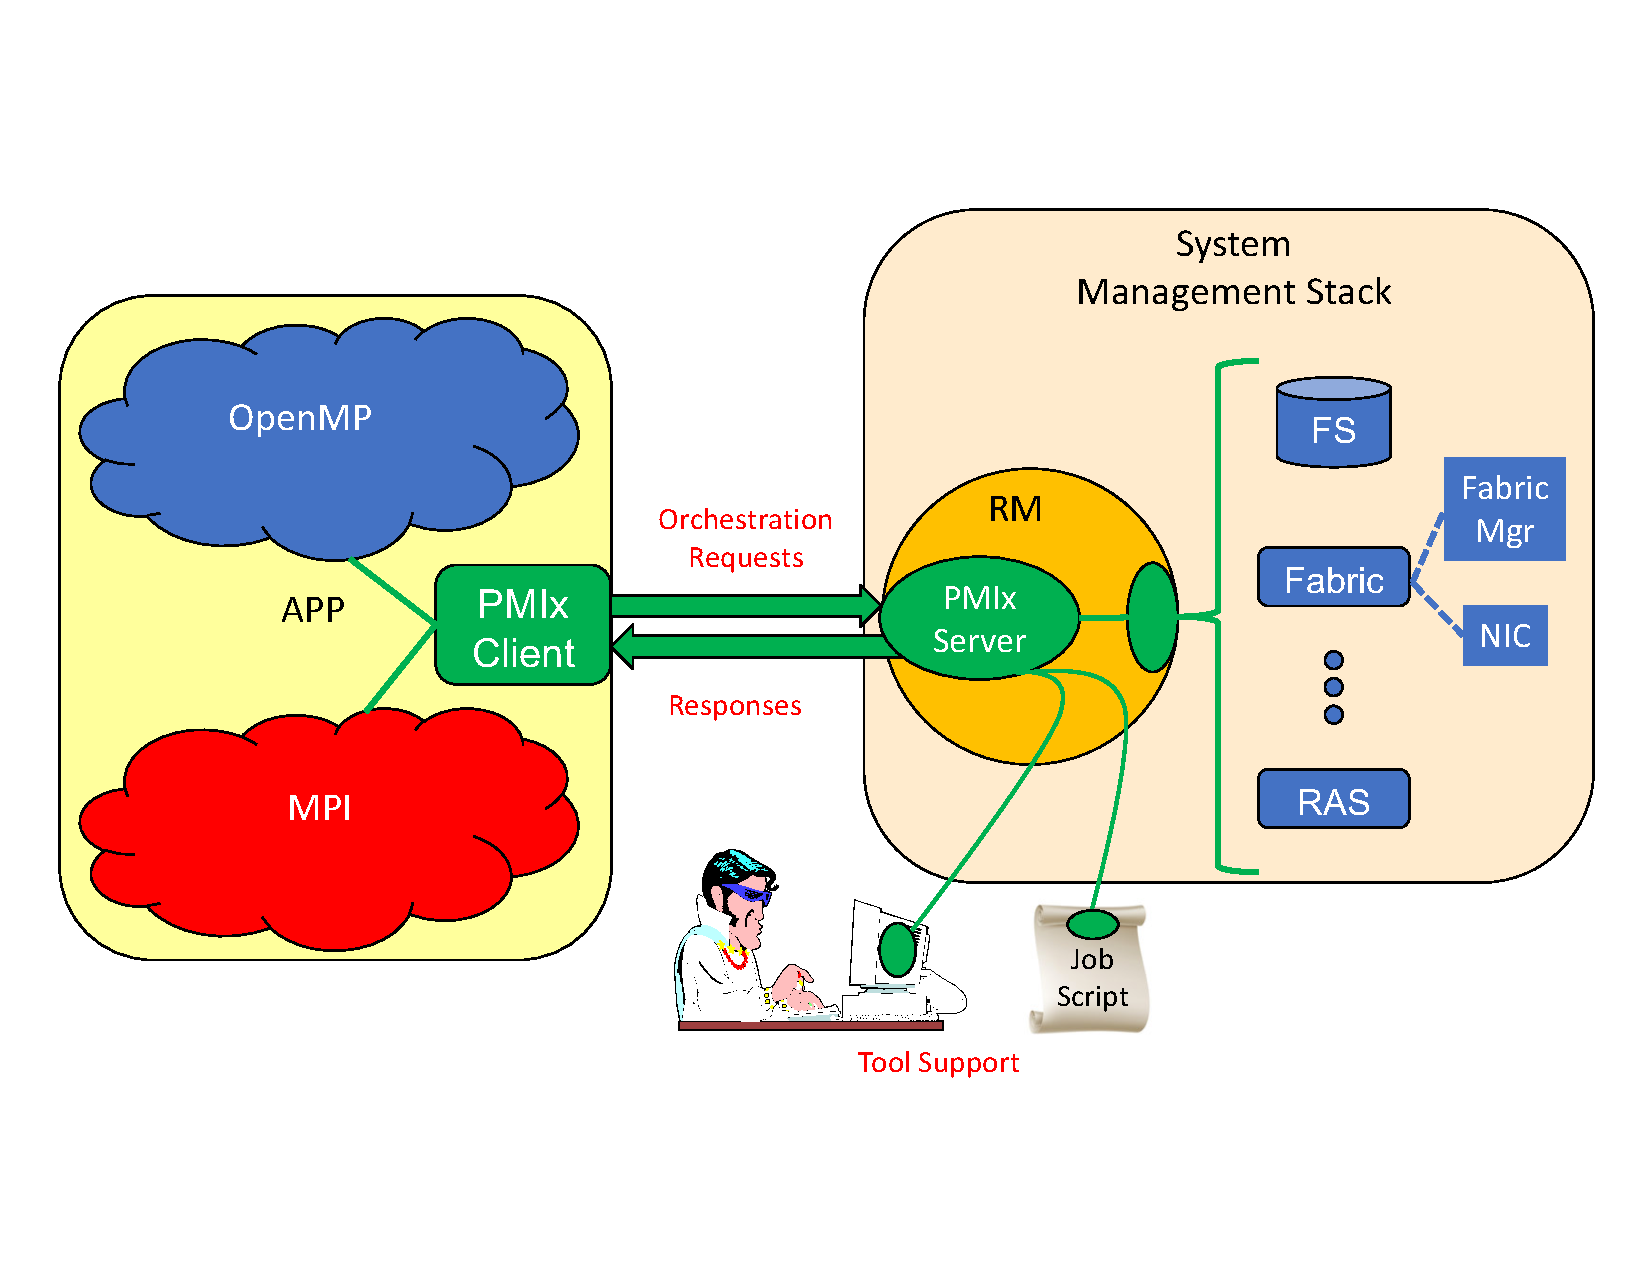
\includegraphics[clip,width=0.8\textwidth]{figs/PMIxRoles.pdf}
  \end{center}
  \caption{PMIx-SMS Interactions}
  \label{fig:roles}
\end{figure*}
\endgroup


Fig.~\ref{fig:roles} shows a typical \ac{PMIx} implementation in which the application is
built against a \ac{PMIx} client library that contains the client-side \acp{API},
attribute definitions, and communication support for interacting with the local \ac{PMIx} server.
\ac{PMIx} clients are processes which are started through the \ac{PMIx} infrastructure,
either by the PMIx implementation directly or through a \ac{SMS} component, and have registered
as clients.  A \ac{PMIx} client
is created in such a way that the \ac{PMIx} client library
will be have sufficient information available to
authenticate with the \ac{PMIx} server.
The \ac{PMIx} server will have sufficient knowledge about the
process which it created, either directly or through other \ac{SMS}, to authenticate the
process and provide information the process requests such as its identity and the
identity of its peers.

As clients invoke \ac{PMIx} \acp{API}, it is possible that some client requests can
be handled at the client level.  Other requests might require communication with the
local \ac{PMIx} server, which subsequently might request services from the host \ac{SMS}
(represented here by a \ac{RM} daemon).
The interaction between the \ac{PMIx} server and \ac{SMS} are
achieved using callback functions registered during server initialization.
The host \ac{SMS} can indicate its lack of support for any operation by simply providing a \textit{NULL} for the associated callback function, or can create a function entry that returns \textit{not supported} when called.

Recognizing the burden this places on SMS vendors, the PMIx community has included interfaces by
which the host \ac{SMS} (containing the local PMIx service instance) can request support from local \ac{SMS} elements via the PMIx API.  Once the \ac{SMS} has transferred the request to
an appropriate location, a \ac{PMIx} server interface can be used to pass the request
between \ac{SMS} subsystems.
For example, a request for network traffic statistics can utilize the
PMIx networking abstractions to retrieve the information from the Fabric Manager.
This reduces the portability and
interoperability issues between the individual subsystems by transferring the burden of defining the
interoperable interfaces from the \ac{SMS} subsystems to the \ac{PMIx} community, which continues
to work with those providers to develop the necessary support.

Fig.~\ref{fig:roles} shows how tools can interact with the \ac{PMIx} architecture.
Tools, whether standalone or embedded in job scripts, are an exception to
the normal client registration process.   A process can register as a tool, provided
the \ac{PMIx} client library has adequate rendezvous information to connect to the appropriate
\ac{PMIx} server (either hosted on the local machine or on a remote machine).  This allows processes
which were not created by the PMIx infrastructure to request access to PMIx functionality.

\section{Portability of Functionality}
\label{chap:intro:not_supported}

It is difficult to define a portable \ac{API} that will provide access to the many
and varied features underlying the operations for which \ac{PMIx} provides access.
For example, the options and features provided to request the creation
of new processes varied dramatically between different systems existing
at the time \ac{PMIx} was introduced.  Many \acp{RM} provide rich interfaces
to specify the resources assigned to processes.
As a result, \ac{PMIx} is faced with the challenge
of attempting to meet the seamingly conflicting goals of creating an \ac{API} which allows
access to these diverse features while being portable across a wide range of
existing software environments. In addition, the functionalities required by different
clients vary greatly.  Producing a \ac{PMIx} implementation
which can provide the needs of all possible clients on all of its target systems
could be so burdensome as to discourage \ac{PMIx} implementations.

To help address this issue, the \ac{PMIx} \acp{API} are designed to allow resource managers
and other system management stack components to decide on support of a
particular function and allow client applications to query and adjust to the level of support available.  \ac{PMIx} clients should be written to account for the possibility that a \ac{PMIx} \ac{API} might return an error code indicating that the call is not supported.
The \ac{PMIx} community continues to look at ways to assist \ac{SMS} implementers in their decisions
on what functionality to support by highlighting functions and attributes that are
critical to basic application execution (e.g., \refapi{PMIx_Get}) for certain classes of applications.

\subsection{Optional Nature of Attributes}

An area where differences between support on different systems can be challenging is regarding the attributes that provide information to the client process and/or control the behavior of a \ac{PMIx} \ac{API}.  Most
\ac{PMIx} \ac{API} calls can accept additional information or attributes specified in the form of
key/value pairs. These attributes provide information to the \ac{PMIx} implementation that influence the
behavior of the \ac{API} call.  In addition to \ac{API} calls being optional, support for the
individual attributes of an \ac{API} call can vary between systems or implementations.

An application can adapt to the attribute support on a particular system in one of two ways.
\ac{PMIx} provides an \ac{API} to enable an application to query the attributes
supported by a particular \ac{API} (See \ref{chap:api_job_mgmt:queryattrs}).
Through this \ac{API}, the \ac{PMIx} implementation can provide detailed information
about the attributes supported on a system for each \ac{API} call queried.
Alternatively, the application can mark attributes as
required using a flag within the \refstruct{pmix_info_t} (See \ref{chap:struct:info}).
If the required attribute is
not available on the system or the desired value for the attribute is not available, the call will
return the error code for \textit{not supported}.

For example, the \refattr{PMIX_TIMEOUT} attribute can be used to specify the time (in seconds) before the requested operation should time out. The intent of this attribute is to allow the client to avoid ``hanging'' in a request that takes longer than the client wishes to wait, or may never return (e.g., a \refapi{PMIx_Fence} that a blocked participant never enters).

The application can query the attribute support for \refapi{PMIx_Fence}
and search whether \refattr{PMIX_TIMEOUT} is listed as a supported attribute.  The application can also
set the required flag in the \refstruct{pmix_info_t} for that attribute when making the \refapi{PMIx_Fence}
call. This will return an error if this attribute is not supported. If the required flag is not set,
the library and \ac{SMS} host are allowed to treat the attribute as optional, ignoring it if support
is not available.

It is therefore critical that users and application implementers:

\begin{compactalphaenum}
\item consider whether or not a given attribute is required, marking it accordingly; and

\item check the return status on all \ac{PMIx} function calls to ensure support was present and that the request was accepted. Note that for non-blocking \acp{API}, a return of \refconst{PMIX_SUCCESS} only indicates that the request had no obvious errors and is being processed – the eventual callback will return the status of the requested operation itself.
\end{compactalphaenum}

\ac{PMIx} clients (e.g., tools, parallel programming libraries) may find that they depend only on a small subset of interfaces and attributes to work correctly.
\ac{PMIx} clients are strongly advised to define a document itemizing the \ac{PMIx} interfaces and associated attributes that are required for correct operation, and are optional but recommended for full functionality.
The \ac{PMIx} standard cannot define this list for all given \ac{PMIx} clients, but such a list is valuable to \acp{RM} desiring to support these clients.

A \ac{PMIx} implementation may be able to support only a subset of the \ac{PMIx} \acs{API} and attributes on
a particular system due to either its own limitations or limitations of the \ac{SMS} with which it interfaces.
A \ac{PMIx} implemenation may also provide additional attributes beyond those defined herein in order to allow
applications to access the full features of the underlying \ac{SMS}.
\ac{PMIx} implementations are strongly advised to document the \ac{PMIx} interfaces and associated attributes they support, with any annotations about behavior limitations.
The \ac{PMIx} standard cannot define this support for implementations, but such documentation is valuable to \ac{PMIx} clients desiring to support a broad range of systems.

While a \ac{PMIx} library implementer, or an \ac{SMS} component server, may choose to support a particular \ac{PMIx} \ac{API}, they are not required to support every attribute that might apply to it. This would pose a significant barrier to entry for an implementer as there can be a broad range of applicable attributes to a given \ac{API}, at least some of which may rarely be used.

Note that an environment that does not include support for a particular attribute/\ac{API} pair is not ``incomplete'' or of lower quality than one that does include that support. Vendors must decide where to invest their time based on the needs of their target markets, and it is perfectly reasonable for them to perform cost/benefit decisions when considering what functions and attributes to support.

%%%%%%%%%%%%%%%%%%%%%%%%%%%%%%%%%%%%%%%%%%%%%%%%%
\section{Organization of this document}

The remainder of this document is structured as follows:

\begin{itemize}
\item Introduction and Overview in \chapterref{chap:intro}
\item Terms and Conventions in \chapterref{chap:terms}
\item Data Structures and Types in \chapterref{chap:struct}
\item \ac{PMIx} Initialization and Finalization in \chapterref{chap:api_init}
\item Key/Value Management in \chapterref{chap:api_kv_mgmt}
\item Process Management in \chapterref{chap:api_proc_mgmt}
\item Job Management in \chapterref{chap:api_job_mgmt}
\item Event Notification in \chapterref{chap:api_event}
\item Data Packing and Unpacking in \chapterref{chap:api_data_mgmt}
\item Security in \chapterref{chap:api_security}
\item \ac{PMIx} Server Specific Interfaces in \chapterref{chap:api_server}
\item Scheduler-Specific Interface in \chapterref{chap:api_scheduler}
\item Process Sets and Groups in \chapterref{chap:api_sets_groups}
\item Network Coordinates in \chapterref{chap:network_coords}
\item Python Bindings in \appendixref{app:python}
\end{itemize}

%%%%%%%%%%%%%%%%%%%%%%%%%%%%%%%%%%%%%%%%%%%%%%%%%
%%%%%%%%%% History: Version 1.0
\section{Version 1.0: June 12, 2015}

\par
The \ac{PMIx} version 1.0 \textit{ad hoc} standard was defined in the \acf{PRI} header files as part of the \ac{PRI} v1.0.0 release prior to the creation of the formal \ac{PMIx} 2.0 standard.
Below are a summary listing of the interfaces defined in the 1.0 headers.

\begin{itemize}
\item Client APIs
\begin{itemize}
\item PMIx\_Init, \refapi{PMIx_Initialized}, \refapi{PMIx_Abort}, \refapi{PMIx_Finalize}
\item \refapi{PMIx_Put}, \refapi{PMIx_Commit},
\item \refapi{PMIx_Fence}, \refapi{PMIx_Fence_nb}
\item \refapi{PMIx_Get}, \refapi{PMIx_Get_nb}
\item \refapi{PMIx_Publish}, \refapi{PMIx_Publish_nb}
\item \refapi{PMIx_Lookup}, \refapi{PMIx_Lookup_nb}
\item \refapi{PMIx_Unpublish}, \refapi{PMIx_Unpublish_nb}
\item \refapi{PMIx_Spawn}, \refapi{PMIx_Spawn_nb}
\item \refapi{PMIx_Connect}, \refapi{PMIx_Connect_nb}
\item \refapi{PMIx_Disconnect}, \refapi{PMIx_Disconnect_nb}
\item \refapi{PMIx_Resolve_nodes}, \refapi{PMIx_Resolve_peers}
\end{itemize}
\item Server \acp{API}
\begin{itemize}
\item \refapi{PMIx_server_init}, \refapi{PMIx_server_finalize}
\item \refapi{PMIx_generate_regex}, \refapi{PMIx_generate_ppn}
\item \refapi{PMIx_server_register_nspace}, \refapi{PMIx_server_deregister_nspace}
\item \refapi{PMIx_server_register_client}, \refapi{PMIx_server_deregister_client}
\item \refapi{PMIx_server_setup_fork}, \refapi{PMIx_server_dmodex_request}
\end{itemize}
\item Common \acp{API}
\begin{itemize}
\item \refapi{PMIx_Get_version}, \refapi{PMIx_Store_internal}, \refapi{PMIx_Error_string}
\item PMIx_Register_errhandler, PMIx_Deregister_errhandler, PMIx_Notify_error
\end{itemize}
\end{itemize}

The \code{PMIx_Init} \ac{API} was subsequently modified in the \ac{PRI} release v1.1.0.

%%%%%%%%%%%%%%%%%%%%%%%%%%%%%%%%%%%%%%%%%%%%%%%%%
%%%%%%%%%% History: Version 2.0
\section{Version 2.0: Sept. 2018}

The following \acp{API} were introduced in v2.0 of the PMIx Standard:

\begin{itemize}
\item Client APIs
\begin{itemize}
\item \refapi{PMIx_Query_info_nb}, \refapi{PMIx_Log_nb}
\item \refapi{PMIx_Allocation_request_nb}, \refapi{PMIx_Job_control_nb}, \refapi{PMIx_Process_monitor_nb}, \refmacro{PMIx_Heartbeat}
\end{itemize}
\item Server \acp{API}
\begin{itemize}
\item \refapi{PMIx_server_setup_application}, \refapi{PMIx_server_setup_local_support}
\end{itemize}
\item Tool \acp{API}
\begin{itemize}
\item \refapi{PMIx_tool_init}, \refapi{PMIx_tool_finalize}
\end{itemize}
\item Common \acp{API}
\begin{itemize}
\item \refapi{PMIx_Register_event_handler}, \refapi{PMIx_Deregister_event_handler}
\item \refapi{PMIx_Notify_event}
\item \refapi{PMIx_Proc_state_string}, \refapi{PMIx_Scope_string}
\item \refapi{PMIx_Persistence_string}, \refapi{PMIx_Data_range_string}
\item \refapi{PMIx_Info_directives_string}, \refapi{PMIx_Data_type_string}
\item \refapi{PMIx_Alloc_directive_string}
\item \refapi{PMIx_Data_pack}, \refapi{PMIx_Data_unpack}, \refapi{PMIx_Data_copy}
\item \refapi{PMIx_Data_print}, \refapi{PMIx_Data_copy_payload}
\end{itemize}
\end{itemize}

The \refapi{PMIx_Init} \ac{API} was modified in v2.0 of the standard from its \textit{ad hoc} v1.0 signature to include passing of a \refstruct{pmix_info_t} array for flexibility and ``future-proofing'' of the \ac{API}.
In addition, the PMIx_Notify_error, PMIx_Register_errhandler, and PMIx_Deregister_errhandler \acp{API} were replaced.

%%%%%%%%%%%%%%%%%%%%%%%%%%%%%%%%%%%%%%%%%%%%%%%%%
%%%%%%%%%% History: Version 2.1
\section{Version 2.1: Dec. 2018}

The v2.1 update includes clarifications and corrections from the v2.0 document, plus addition of examples:

\begin{itemize}
    \item Clarify description of \refapi{PMIx_Connect} and \refapi{PMIx_Disconnect} \acp{API}.
    \item Explain that values for the \refattr{PMIX_COLLECTIVE_ALGO} are environment-dependent
    \item Identify the namespace/rank values required for retrieving attribute-associated information using the \refapi{PMIx_Get} \ac{API}
    \item Provide definitions for \refterm{session}, \refterm{job}, \refterm{application}, and other terms used throughout the document
    \item Clarify definitions of \refattr{PMIX_UNIV_SIZE} versus \refattr{PMIX_JOB_SIZE}
    \item Clarify server module function return values
    \item Provide examples of the use of \refapi{PMIx_Get} for retrieval of information
    \item Clarify the use of \refapi{PMIx_Get} versus \refapi{PMIx_Query_info_nb}
    \item Clarify return values for non-blocking \acp{API} and emphasize that callback functions must not be invoked prior to return from the \ac{API}
    \item Provide detailed example for construction of the \refapi{PMIx_server_register_nspace} input information array
    \item Define information levels (e.g., \refterm{session} vs \refterm{job}) and associated attributes for both storing and retrieving values
    \item Clarify roles of \ac{PMIx} server library and host environment for collective operations
    \item Clarify definition of \refattr{PMIX_UNIV_SIZE}
\end{itemize}

%%%%%%%%%%%%%%%%%%%%%%%%%%%%%%%%%%%%%%%%%%%%%%%%%
%%%%%%%%%% History: Version 2.2
\section{Version 2.2: Jan 2019}

The v2.2 update includes the following clarifications and corrections from the v2.1 document:

\begin{itemize}
    \item Direct modex upcall function (\refapi{pmix_server_dmodex_req_fn_t}) cannot complete atomically as the \ac{API} cannot return the requested information except via the provided callback function
    \item Add missing \refstruct{pmix_data_array_t} definition and support macros
    \item Add a rule divider between implementer and host environment required attributes for clarity
    \item Add \refmacro{PMIX_QUERY_QUALIFIERS_CREATE} macro to simplify creation of \refstruct{pmix_query_t} qualifiers
    \item Add \refmacro{PMIX_APP_INFO_CREATE} macro to simplify creation of \refstruct{pmix_app_t} directives
    \item Add flag and \refmacro{PMIX_INFO_IS_END} macro for marking and detecting the end of a \refstruct{pmix_info_t} array
    \item Clarify the allowed hierarchical nesting of the \refattr{PMIX_SESSION_INFO_ARRAY}, \refattr{PMIX_JOB_INFO_ARRAY}, and associated attributes
\end{itemize}

%%%%%%%%%%%%%%%%%%%%%%%%%%%%%%%%%%%%%%%%%%%%%%%%%
%%%%%%%%%% History: Version 3.0
\section{Version 3.0: Dec. 2018}

The following \acp{API} were introduced in v3.0 of the PMIx Standard:

\begin{itemize}
\item Client APIs
\begin{itemize}
\item \refapi{PMIx_Log}, \refapi{PMIx_Job_control}
\item \refapi{PMIx_Allocation_request}, \refapi{PMIx_Process_monitor}
\item \refapi{PMIx_Get_credential}, \refapi{PMIx_Validate_credential}
\end{itemize}
\item Server \acp{API}
\begin{itemize}
\item \refapi{PMIx_server_IOF_deliver}
\item \refapi{PMIx_server_collect_inventory}, \refapi{PMIx_server_deliver_inventory}
\end{itemize}
\item Tool \acp{API}
\begin{itemize}
\item \refapi{PMIx_IOF_pull}, \refapi{PMIx_IOF_push}, \refapi{PMIx_IOF_deregister}
\item \refapi{PMIx_tool_connect_to_server}
\end{itemize}
\item Common \acp{API}
\begin{itemize}
\item \refapi{PMIx_IOF_channel_string}
\end{itemize}
\end{itemize}

The document added a chapter on security credentials, a new section for \ac{IO} forwarding to the Process Management chapter, and a few blocking forms of previously-existing non-blocking \acp{API}. Attributes supporting the new \acp{API} were introduced, as well as additional attributes for a few existing functions.

%%%%%%%%%%%%%%%%%%%%%%%%%%%%%%%%%%%%%%%%%%%%%%%%%
%%%%%%%%%% History: Version 3.1
\section{Version 3.1: Jan. 2019}

The v3.1 update includes clarifications and corrections from the v3.0 document:

\begin{itemize}
    \item Direct modex upcall function (\refapi{pmix_server_dmodex_req_fn_t}) cannot complete atomically as the \ac{API} cannot return the requested information except via the provided callback function
    \item Fix typo in name of \refattr{PMIX_FWD_STDDIAG} attribute
    \item Correctly identify the information retrieval and storage attributes as ``new'' to v3 of the standard
    \item Add missing \refstruct{pmix_data_array_t} definition and support macros
    \item Add a rule divider between implementer and host environment required attributes for clarity
    \item Add \refmacro{PMIX_QUERY_QUALIFIERS_CREATE} macro to simplify creation of \refstruct{pmix_query_t} qualifiers
    \item Add \refmacro{PMIX_APP_INFO_CREATE} macro to simplify creation of \refstruct{pmix_app_t} directives
    \item Add new attributes to specify the level of information being requested where ambiguity may exist (see \ref{api:struct:attributes:retrieval})
    \item Add new attributes to assemble information by its level for storage where ambiguity may exist (see \ref{api:struct:attributes:storage})
    \item Add flag and \refmacro{PMIX_INFO_IS_END} macro for marking and detecting the end of a \refstruct{pmix_info_t} array
    \item Clarify that \code{PMIX_NUM_SLOTS} is duplicative of (a) \refattr{PMIX_UNIV_SIZE} when used at the \refterm{session} level and (b) \refattr{PMIX_MAX_PROCS} when used at the \refterm{job} and \refterm{application} levels, but leave it in for backward compatibility.
    \item Clarify difference between \refattr{PMIX_JOB_SIZE} and \refattr{PMIX_MAX_PROCS}
    \item Clarify that \refapi{PMIx_server_setup_application} must be called per-\refterm{job} instead of per-\refterm{application} as the name implies. Unfortunately, this is a historical artifact. Note that both \refattr{PMIX_NODE_MAP} and \refattr{PMIX_PROC_MAP} must be included as input in the \refarg{info} array provided to that function. Further descriptive explanation of the ``instant on'' procedure will be provided in the next version of the \ac{PMIx} Standard.
    \item Clarify how the \ac{PMIx} server expects data passed to the host by \refapi{pmix_server_fencenb_fn_t} should be aggregated across nodes, and provide a code snippet example
\end{itemize}


%%%%%%%%%%%%%%%%%%%%%%%%%%%%%%%%%%%%%%%%%%%%%%%%%
%%%%%%%%%% History: Version 3.2
\section{Version 3.2: Oct. 2019}

The v3.2 update includes clarifications and corrections from the v3.1 document:

\begin{itemize}
    \item Correct an error in the \refapi{PMIx_Allocation_request} function signature, and clarify the allocation ID attributes
    \item Rename the \refattr{PMIX_ALLOC_ID} attribute to \refattr{PMIX_ALLOC_REQ_ID} to clarify that this is a string the user provides as a means to identify their request to query status
    \item Add a new \refattr{PMIX_ALLOC_ID} attribute that contains the identifier (provided by the host environment) for the resulting allocation which can later be used to reference the allocated resources in, for example, a call to \refapi{PMIx_Spawn}
\end{itemize}


%%%%%%%%%%%%%%%%%%%%%%%%%%%%%%%%%%%%%%%%%%%%%%%%%
%%%%%%%%%% History: Version 4.0
\section{Version 4.0: Sept 2020}


The following changes were introduced in v4.0 of the PMIx Standard:

\begin{itemize}
    \item Clarified that the \refapi{PMIx_Fence_nb} operation can immediately return \refconst{PMIX_OPERATION_SUCCEEDED} in lieu of passing the request to a \ac{PMIx} server if only the calling process is involved in the operation
    \item Added the \refapi{PMIx_Register_attributes} \ac{API} by which a host environment can register the attributes it supports for each server-to-host operation
    \item Added the ability to query supported attributes from the \ac{PMIx} tool, client and server libraries, as well as the host environment via the new \refstruct{pmix_regattr_t} structure. Both human-readable and machine-parsable output is supported. New attributes to support this operation include:
    \begin{itemize}
        \item \refattr{PMIX_CLIENT_ATTRIBUTES}, \refattr{PMIX_SERVER_ATTRIBUTES}, \refattr{PMIX_TOOL_ATTRIBUTES}, and \refattr{PMIX_HOST_ATTRIBUTES} to identify which library supports the attribute; and
        \item \refattr{PMIX_MAX_VALUE}, \refattr{PMIX_MIN_VALUE}, and \refattr{PMIX_ENUM_VALUE} to provide machine-parsable description of accepted values
    \end{itemize}
    \item Add \refconst{PMIX_APP_WILDCARD} to reference all applications within a given job
    \item Fix signature of blocking APIs \refapi{PMIx_Allocation_request}, \refapi{PMIx_Job_control}, \refapi{PMIx_Process_monitor}, \refapi{PMIx_Get_credential}, and \refapi{PMIx_Validate_credential} to allow return of results
    \item Update description to provide an option for blocking behavior of the \refapi{PMIx_Register_event_handler}, \refapi{PMIx_Deregister_event_handler}, \refapi{PMIx_Notify_event}, \refapi{PMIx_IOF_pull}, \refapi{PMIx_IOF_deregister}, and \refapi{PMIx_IOF_push} APIs. The need for blocking forms of these functions was not initially anticipated but has emerged over time. For these functions, the return value is sufficient to provide the caller with information otherwise returned via callback. Thus, use of a \code{NULL} value as the callback function parameter was deemed a minimal disruption method for providing the desired capability
    \item Added a chapter on fabric support that includes new \acp{API}, datatypes, and attributes
    \item Added a chapter on process sets and groups that includes new \acp{API} and attributes
    \item Added \acp{API} and a new datatype to support generation and parsing of \ac{PMIx} locality strings
    \item Added a new chapter on tools that provides deeper explanation on their operation and collecting all tool-relevant definitions into one location. Also introduced two new \acp{API} and removed restriction that limited tools to being connected to only one server at a time.
\end{itemize}

The above changes included introduction of the following \acp{API}:

\begin{itemize}
    \item Client APIs
    \begin{itemize}
        \item \refapi{PMIx_Group_construct}, \refapi{PMIx_Group_construct_nb}
        \item \refapi{PMIx_Group_destruct}, \refapi{PMIx_Group_destruct_nb}
        \item \refapi{PMIx_Group_invite}, \refapi{PMIx_Group_invite_nb}
        \item \refapi{PMIx_Group_join}, \refapi{PMIx_Group_join_nb}
        \item \refapi{PMIx_Group_leave}, \refapi{PMIx_Group_leave_nb}
        \item \refapi{PMIx_get_relative_locality}
    \end{itemize}

    \item Server \acp{API}
    \begin{itemize}
    \item \refapi{PMIx_Fabric_register}, \refapi{PMIx_Fabric_register_nb}
    \item \refapi{PMIx_Fabric_update}, \refapi{PMIx_Fabric_update_nb}
    \item \refapi{PMIx_Fabric_deregister}, \refapi{PMIx_Fabric_deregister_nb}
    \item \refapi{PMIx_Fabric_get_vertex_info}, \refapi{PMIx_Fabric_get_vertex_info_nb}
    \item \refapi{PMIx_Fabric_get_device_index}, \refapi{PMIx_Fabric_get_device_index_nb}
    \item \refapi{PMIx_generate_locality_string}
    \item \refapi{PMIx_Register_attributes}
    \item \refapi{pmix_server_grp_fn_t}, \refapi{pmix_server_fabric_fn_t}
    \end{itemize}

    \item Tool \acp{API}
    \begin{itemize}
    \item \refapi{PMIx_tool_disconnect}
    \item \refapi{PMIx_tool_set_server}
    \end{itemize}
\end{itemize}


    % PMIx Terms and Conventions
    %%%%%%%%%%%%%%%%%%%%%%%%%%%%%%%%%%%%%%%%%%%%%%%%%
% Chapter: Terms and Conventions
%%%%%%%%%%%%%%%%%%%%%%%%%%%%%%%%%%%%%%%%%%%%%%%%%
\chapter{PMIx Terms and Conventions}
\label{chap:terms}

The \ac{PMIx} Standard has adopted the widespread use of key-value \textit{attributes} to add flexibility to the functionality expressed in the existing \acp{API}. Accordingly, the community has chosen to require that the definition of each standard \ac{API} include the passing of an array of attributes. These provide a means of customizing the behavior of the \ac{API} as future needs emerge without having to alter or create new variants of it. In addition, attributes provide a mechanism by which researchers can easily explore new approaches to a given operation without having to modify the \ac{API} itself.

The \ac{PMIx} community has further adopted a policy that modification of existing released \acp{API} will only be permitted under extreme circumstances. In its effort to avoid introduction of any such backward incompatibility, the community has avoided the definitions of large numbers of \acp{API} that each focus on a narrow scope of functionality, and instead relied on the definition of fewer generic \acp{API} that include arrays of directives for ``tuning'' the function's behavior. Thus, modifications to the PMIx standard increasingly consist of the definition of new attributes along with a description of the \acp{API} to which they relate and the expected behavior when used with those \acp{API}.

One area where this can become more complicated relates to the attributes that provide directives to the client process and/or control the behavior of a \ac{PMIx} standard \ac{API}. For example, the \refattr{PMIX_TIMEOUT} attribute can be used to specify the time (in seconds) before the requested operation should time out.
The intent of this attribute is to allow the client to avoid hanging in a request that takes longer than the client wishes to wait, or may never return (e.g., a \refapi{PMIx_Fence} that a blocked participant never enters).

If an application truly relies on the \refattr{PMIX_TIMEOUT} attribute in a call to \refapi{PMIx_Fence}, it should set the \textit{required} flag in the \refstruct{pmix_info_t} for that attribute. This informs the library and its \ac{SMS} host that it must return an immediate error if this attribute is not supported. By not setting the flag, the library and \ac{SMS} host are allowed to treat the attribute as optional, silently ignoring it if support is not available.

\adviceuserstart
It is critical that users and application developers consider whether or not a given attribute is required (marking it accordingly) and always check the return status on all \ac{PMIx} function calls to ensure support was present and that the request was accepted. Note that for non-blocking \acp{API}, a return of \refconst{PMIX_SUCCESS} only indicates that the request had no obvious errors and is being processed. The eventual callback will return the status of the requested operation itself.
\adviceuserend

While a \ac{PMIx} library implementer, or an \ac{SMS} component server, may choose to support a particular \ac{PMIx} \ac{API}, they are not required to support every attribute that might apply to it. This would pose a significant barrier to entry for an implementer as there can be a broad range of applicable attributes to a given \ac{API}, at least some of which may rarely be used in a specific market area. The \ac{PMIx} community is attempting to help differentiate the attributes by indicating in the standard those that are generally used (and therefore, of higher importance to support) versus those that a ``complete implementation'' would support.

In addition, the document refers to the following entities and process stages when describing use-cases or operations involving \ac{PMIx}:

\begin{itemize}
\item \declareterm{session}\emph{session} refers to an allocated set of resources assigned to a particular user by the system \ac{WLM}. Historically, \ac{HPC} sessions have consisted of a static allocation of resources - i.e., a block of resources are assigned to a user in response to a specific request and managed as a unified collection. However, this is changing in response to the growing use of dynamic programming models that require on-the-fly allocation and release of system resources. Accordingly, the term \emph{session} in this document refers to the current block of assigned resources and is a potentially dynamic entity.
\item \declareterm{slot}\declareterm{slots}\emph{slot} refers to an allocated entry for a process. \acp{WLM} frequently allocate entire nodes to a \emph{session}, but can also be configured to define the maximum number of processes that can simultaneously be executed on each node. This often corresponds to the number of hardware \acp{PU} (typically cores, but can also be defined as hardware threads) on the node. However, the correlation between hardware \acp{PU} and slot allocations strictly depends upon system configuration.
\item \declareterm{job}\emph{job} refers to a set of one or more \emph{applications} executed as a single invocation by the user within a session. For example, ``\textit{mpiexec -n 1 app1 : -n 2 app2}'' is considered a single \ac{MPMD} job containing two applications.
\item \declareterm{namespace}\emph{namespace} refers to a character string value assigned by the \ac{RM} to a \textit{job}. All \textit{applications} executed as part of that \textit{job} share the same \emph{namespace}. The \emph{namespace} assigned to each \emph{job} must be unique within the scope of the governing \ac{RM}.
\item \declareterm{application}\emph{application} refers to a single executable (binary, script, etc.) member of a \emph{job}. Applications consist of one or more \emph{processes}, either operating independently or in parallel at any given time during their execution.
\item \declareterm{rank}\emph{rank} refers to the numerical location (starting from zero) of a process within the defined scope. Thus, {global rank} is the rank of a process within its \emph{job}, while \emph{application rank} is the rank of that process within its \emph{application}.
\item \declareterm{workflow}\declareterm{workflows}\emph{workflow} refers to an orchestrated execution plan frequently spanning multiple \emph{jobs} carried out under the control of a \emph{workflow manager} process. An example workflow might first execute a computational job to generate the flow of liquid through a complex cavity, followed by a visualization job that takes the output of the first job as its input to produce an image output.
\item \declareterm{scheduler}\emph{scheduler} refers to the component of the \ac{SMS} responsible for scheduling of resource allocations. This is also generally referred to as the \emph{system workflow manager} - for the purposes of this document, the \emph{WLM} acronym will be used interchangeably to refer to the scheduler.
\item \declareterm{resource manager}\emph{resource manager} is used in a generic sense to represent the subsystem that will host the \ac{PMIx} server library. This could be a vendor's \ac{RM}, a programming library's \ac{RTE}, or some other agent.
\item \declareterm{host environment}\emph{host environment} is used interchangeably with \emph{resource manager} to refer to the process hosting the \ac{PMIx} server library.
\item \declareterm{network plane}\declareterm{network planes}\emph{network plane} refers to a collection of \acp{NIC} and switches in a common logical or physical configuration. Network planes are often implemented in \ac{HPC} clusters as separate overlay or physical networks controlled by a dedicated fabric manager.
\end{itemize}


This document borrows freely from other standards (most notably from the \ac{MPI} and OpenMP standards) in its use of notation and conventions in an attempt to reduce confusion. The following sections provide an overview of the conventions used throughout the \ac{PMIx} Standard document.

%%%%%%%%%%%
\section{Notational Conventions}

Some sections of this document describe programming language specific examples or \acp{API}.
Text that applies only to programs for which the base language is C is shown as follows:

\cspecificstart
C specific text...
\begin{codepar}
int foo = 42;
\end{codepar}
\cspecificend

Some text is for information only, and is not part of the normative specification.
These take several forms, described in their examples below:

\notestart
\noteheader
General text...
\noteend

\rationalestart
Throughout this document, the rationale for the design choices made in the interface specification is set off in this section.
Some readers may wish to skip these sections, while readers interested in interface design may want to read them carefully.
\rationaleend

\adviceuserstart
Throughout this document, material aimed at users and that illustrates usage is set off in this section.
Some readers may wish to skip these sections, while readers interested in programming with the \ac{PMIx} \ac{API} may want to read them carefully.
\adviceuserend

\adviceimplstart
Throughout this document, material that is primarily commentary to \ac{PMIx} library implementers is set off in this section.
Some readers may wish to skip these sections, while readers interested in \ac{PMIx} implementations may want to read them carefully.
\adviceimplend

\advicermstart
Throughout this document, material that is primarily commentary aimed at host environments (e.g., \acp{RM} and \acp{RTE}) providing support for the \ac{PMIx} server library is set off in this section.
Some readers may wish to skip these sections, while readers interested in integrating \ac{PMIx} servers into their environment may want to read them carefully.
\advicermend

%%%%%%%%%%%
\section{Semantics}

The following terms will be taken to mean:

\begin{itemize}
\item \emph{shall}, \emph{must} and \emph{will} indicate that the specified behavior is \emph{required} of all conforming implementations
\item \emph{should} and \emph{may} indicate behaviors that a complete implementation would include, but are not required of all conforming implementations
\end{itemize}

%%%%%%%%%%%
\section{Naming Conventions}

The \ac{PMIx} standard has adopted the following conventions:

\begin{itemize}
\item \ac{PMIx} constants and attributes are prefixed with \textbf{\code{PMIX}}.
\item Structures and type definitions are prefixed with \code{pmix}.
\item Underscores are used to separate words in a function or variable name.
\item Lowercase letters are used in \ac{PMIx} client \acp{API} except for the \ac{PMIx} prefix (noted below) and the first letter of the word following it.
For example, \refapi{PMIx_Get_version}.
\item \ac{PMIx} server and tool \acp{API} are all lower case letters following the prefix - e.g., \refapi{PMIx_server_register_nspace}.
\item The \code{PMIx_} prefix is used to denote functions.
\item The \code{pmix_} prefix is used to denote function pointer and type definitions.
\end{itemize}

Users should not use the \textbf{\code{PMIX}}, \textbf{\code{PMIx}}, or \textbf{\code{pmix}} prefixes in their applications or libraries so as to avoid symbol conflicts with current and later versions of the \ac{PMIx} standard and implementations such as the \ac{PRI}.

%%%%%%%%%%%
\section{Procedure Conventions}

While the current \acf{PRI} is solely based on the C programming language, it is not the intent of the \ac{PMIx} Standard to preclude the use of other languages.
Accordingly, the procedure specifications in the \ac{PMIx} Standard are written in a language-independent syntax with the arguments marked as IN, OUT, or INOUT.
The meanings of these are:
\begin{itemize}
\item IN:
The call may use the input value but does not update the argument from the perspective of the caller at any time during the calls execution,
\item OUT:
The call may update the argument but does not use its input value
\item INOUT:
The call may both use and update the argument.
\end{itemize}

%%%%%%%%%%%%%%%%%%%%%%%%%%%%%%%%%%%%%%%%%%%%%%%%%
\section{Standard vs Reference Implementation}

The \textit{PMIx Standard} is implementation independent. The \textit{PMIx Reference Implementation} (PRI) is one implementation of the Standard and the \ac{PMIx} community strives to ensure that it fully implements the Standard. Given its role as the community's testbed and its widespread use, this document cites the attributes supported by the \ac{PRI} for each \ac{API} where relevant by marking them in {\color{red}red}. This is not meant to imply nor confer any special role to the \ac{PRI} with respect to the Standard itself, but instead to provide a convenience to users of the Standard and \ac{PRI}.

Similarly, the \textit{PMIx Reference RunTime Environment} (PRRTE) is provided by the community to enable users operating in non-\ac{PMIx} environments to develop and execute \ac{PMIx}-enabled applications and tools. Attributes supported by the \ac{PRRTE} are marked in {\color{green!60!black}green}.



    % Data Structures, Types, Constants
    %  - Includes: Reserved attributes, Keys
    %%%%%%%%%%%%%%%%%%%%%%%%%%%%%%%%%%%%%%%%%%%%%%%%%
% Chapter: Data Structures
%%%%%%%%%%%%%%%%%%%%%%%%%%%%%%%%%%%%%%%%%%%%%%%%%
\chapter{Data Structures and Types}
\label{chap:struct}

This chapter defines PMIx standard data structures, types, and constants.
These apply to all consumers of the PMIx interface.
Where necessary for clarification the description of, for example, an attribute may be copied from this chapter into a section where it is used.

A PMIx implementation may define additional attributes beyond those specified in this document.

\adviceimplstart
If a PMIx implementation chooses to define additional attributes they should avoid using the \code{PMIX} prefix.
This helps the end user distinguish between what is defined by the PMIx standard and what is specific to that PMIx implementation.
\adviceimplend


%%%%%%%%%%%
\section{Constants}

\ac{PMIx} defines a few values that are used throughout the standard to set the size of fixed arrays or as a means of identifying values with special meaning.
The community makes every attempt to minimize the number of such definitions.
The constants defined in this section may be used before calling any \ac{PMIx} library initialization routine.
Additional constants associated with specific data structures or types are defined in the section describing that data structure or type.

\begin{constantdesc}
%
\declareconstitemvalue{PMIX_MAX_NSLEN}{255}
Maximum namespace string length as an integer.
%
\declareconstitemvalue{PMIX_MAX_KEYLEN}{511}
Maximum key string length as an integer.
%
\end{constantdesc}

%%%%%%%%%%%
\subsection{Error Constants}
\label{api:struct:errors}
\declarestruct{pmix_status_t}

The \refstruct{pmix_status_t} structure is a \code{int} type for return status.

The tables shown in this section define the possible values for \refstruct{pmix_status_t}.
PMIx errors are always negative, with 0 reserved for \refconst{PMIX_SUCCESS}.

A PMIx implementation must define all of the constants defined in this section, even if they will never return the specific value to the caller.

%%%%%%%%%%%
\subsubsection{PMIx v1 Error Constants}

The table below represents those constants defined in the PMIx v1 standard.
Those values in this table that were deprecated in later standards are denoted as such.
\ac{PMIx} errors are always negative, with \code{0} reserved for success.

\begin{constantdesc}
%
\declareconstitem{PMIX_SUCCESS}
Success
%
\declareconstitem{PMIX_ERROR}
General Error
%
\declareconstitem{PMIX_ERR_SILENT}
Silent error
%
\declareconstitem{PMIX_ERR_DEBUGGER_RELEASE}
Error in debugger release
%
\declareconstitem{PMIX_ERR_PROC_RESTART}
Fault tolerance: Error in process restart
%
\declareconstitem{PMIX_ERR_PROC_CHECKPOINT}
Fault tolerance: Error in process checkpoint
%
\declareconstitem{PMIX_ERR_PROC_MIGRATE}
Fault tolerance: Error in process migration
%
\declareconstitem{PMIX_ERR_PROC_ABORTED}
Process was aborted
%
\declareconstitem{PMIX_ERR_PROC_REQUESTED_ABORT}
Process is already requested to abort
%
\declareconstitem{PMIX_ERR_PROC_ABORTING}
Process is being aborted
%
\declareconstitem{PMIX_ERR_SERVER_FAILED_REQUEST}
Failed to connect to the server
%
\declareconstitem{PMIX_EXISTS}
(undefined)
%
\declareconstitem{PMIX_ERR_INVALID_CRED}
Invalid security credentials
%
\declareconstitem{PMIX_ERR_HANDSHAKE_FAILED}
Connection handshake failed
%
\declareconstitem{PMIX_ERR_READY_FOR_HANDSHAKE}
Ready for handshake
%
\declareconstitem{PMIX_ERR_WOULD_BLOCK}
Operation would block
%
\declareconstitem{PMIX_ERR_UNKNOWN_DATA_TYPE}
Unknown data type
%
\declareconstitem{PMIX_ERR_PROC_ENTRY_NOT_FOUND}
Process not found
%
\declareconstitem{PMIX_ERR_TYPE_MISMATCH}
Invalid type
%
\declareconstitem{PMIX_ERR_UNPACK_INADEQUATE_SPACE}
Inadequate space to unpack data
%
\declareconstitem{PMIX_ERR_UNPACK_FAILURE}
Unpack failed
%
\declareconstitem{PMIX_ERR_PACK_FAILURE}
Pack failed
%
\declareconstitem{PMIX_ERR_PACK_MISMATCH}
Pack mismatch
%
\declareconstitem{PMIX_ERR_NO_PERMISSIONS}
No permissions
%
\declareconstitem{PMIX_ERR_TIMEOUT}
Timeout expired
%
\declareconstitem{PMIX_ERR_UNREACH}
Unreachable
%
\declareconstitem{PMIX_ERR_IN_ERRNO}
Error defined in \code{errno}
%
\declareconstitem{PMIX_ERR_BAD_PARAM}
Bad parameter
%
\declareconstitem{PMIX_ERR_RESOURCE_BUSY}
Resource busy
%
\declareconstitem{PMIX_ERR_OUT_OF_RESOURCE}
Resource exhausted
%
\declareconstitem{PMIX_ERR_DATA_VALUE_NOT_FOUND}
Data value not found
%
\declareconstitem{PMIX_ERR_INIT}
Error during initialization
%
\declareconstitem{PMIX_ERR_NOMEM}
Out of memory
%
\declareconstitem{PMIX_ERR_INVALID_ARG}
Invalid argument
%
\declareconstitem{PMIX_ERR_INVALID_KEY}
Invalid key
%
\declareconstitem{PMIX_ERR_INVALID_KEY_LENGTH}
Invalid key length
%
\declareconstitem{PMIX_ERR_INVALID_VAL}
Invalid value
%
\declareconstitem{PMIX_ERR_INVALID_VAL_LENGTH}
Invalid value length
%
\declareconstitem{PMIX_ERR_INVALID_LENGTH}
Invalid argument length
%
\declareconstitem{PMIX_ERR_INVALID_NUM_ARGS}
Invalid number of arguments
%
\declareconstitem{PMIX_ERR_INVALID_ARGS}
Invalid arguments
%
\declareconstitem{PMIX_ERR_INVALID_NUM_PARSED}
Invalid number parsed
%
\declareconstitem{PMIX_ERR_INVALID_KEYVALP}
Invalid key/value pair
%
\declareconstitem{PMIX_ERR_INVALID_SIZE}
Invalid size
%
\declareconstitem{PMIX_ERR_INVALID_NAMESPACE}
Invalid namespace
%
\declareconstitem{PMIX_ERR_SERVER_NOT_AVAIL}
Server is not available
%
\declareconstitem{PMIX_ERR_NOT_FOUND}
Not found
%
\declareconstitem{PMIX_ERR_NOT_SUPPORTED}
Not supported
%
\declareconstitem{PMIX_ERR_NOT_IMPLEMENTED}
Not implemented
%
\declareconstitem{PMIX_ERR_COMM_FAILURE}
Communication failure
%
\declareconstitem{PMIX_ERR_UNPACK_READ_PAST_END_OF_BUFFER}
Unpacking past the end of the buffer provided
%
\end{constantdesc}

%%%%%%%%%%%
\subsubsection{PMIx v2 Error Constants}

The table below represents those additional constants defined in the PMIx v2 standard.

\begin{constantdesc}
%
\declareconstitemvalue{PMIX_ERR_V2X_BASE}{-100}
The starting point for v2 error values.
%
\declareconstitem{PMIX_ERR_LOST_CONNECTION_TO_SERVER}
Lost connection to server
%
\declareconstitem{PMIX_ERR_LOST_PEER_CONNECTION}
Lost connection to peer
%
\declareconstitem{PMIX_ERR_LOST_CONNECTION_TO_CLIENT}
Lost connection to client
%
\declareconstitem{PMIX_QUERY_PARTIAL_SUCCESS}
Query partial success (used by query system)
%
\declareconstitem{PMIX_NOTIFY_ALLOC_COMPLETE}
Notify that allocation is complete
%
\declareconstitem{PMIX_JCTRL_CHECKPOINT}
Job control: Monitored by PMIx client to trigger checkpoint operation
%
\declareconstitem{PMIX_JCTRL_CHECKPOINT_COMPLETE}
Job control: Sent by PMIx client and monitored by PMIx server to notify that requested checkpoint operation has completed.
%
\declareconstitem{PMIX_JCTRL_PREEMPT_ALERT}
Job control: Monitored by PMIx client to detect an \ac{RM} intending to preempt the job.
%
\declareconstitem{PMIX_MONITOR_HEARTBEAT_ALERT}
Job monitoring: Heartbeat alert
%
\declareconstitem{PMIX_MONITOR_FILE_ALERT}
Job monitoring: File alert
%
\end{constantdesc}

The table below are operational error constants introduced in the v2 standard.

\begin{constantdesc}
%
\declareconstitemvalue{PMIX_ERR_OP_BASE}{PMIX_ERR_V2X_BASE-30}
The starting point for v2 operational error values.
%
\declareconstitem{PMIX_ERR_EVENT_REGISTRATION}
Error in event registration
%
\declareconstitem{PMIX_ERR_JOB_TERMINATED}
Error job terminated
%
\declareconstitem{PMIX_ERR_UPDATE_ENDPOINTS}
Error updating endpoints
%
\declareconstitem{PMIX_MODEL_DECLARED}
Model declared
%
\declareconstitem{PMIX_GDS_ACTION_COMPLETE}
The \ac{GDS} action has completed
%
\end{constantdesc}

The table below are system error constants introduced in the v2 standard.

\begin{constantdesc}
%
\declareconstitemvalue{PMIX_ERR_SYS_BASE}{PMIX_ERR_OP_BASE-100}
The starting point for v2 system error values.
%
\declareconstitem{PMIX_ERR_NODE_DOWN}
Node down
%
\declareconstitem{PMIX_ERR_NODE_OFFLINE}
Node is marked as offline
%
\end{constantdesc}

The table below are event handler error constants introduced in the v2 standard.

\begin{constantdesc}
%
\declareconstitemvalue{PMIX_ERR_EVHDLR_BASE}{PMIX_ERR_SYS_BASE-100}
The starting point for v2 event handler error values.
%
\declareconstitem{PMIX_EVENT_NO_ACTION_TAKEN}
Event handler: No action taken
%
\declareconstitem{PMIX_EVENT_PARTIAL_ACTION_TAKEN}
Event handler: Partial action taken
%
\declareconstitem{PMIX_EVENT_ACTION_DEFERRED}
Event handler: Action deferred
%
\declareconstitem{PMIX_EVENT_ACTION_COMPLETE}
Event handler: Action complete
%
\end{constantdesc}

Additional error code boundary constants include:

\begin{constantdesc}
%
\declareconstitemvalue{PMIX_INTERNAL_ERR_BASE}{-1000}
A starting point for PMIx internal error codes that are never exposed outside the \ac{PRI}.
%
\declareconstitemvalue{PMIX_EXTERNAL_ERR_BASE}{-2000}
A starting point for user-level defined error constants.
Negative values larger than this are guaranteed not to conflict with PMIx values.
Definitions should always be based on the \refconst{PMIX_EXTERNAL_ERR_BASE} constant and \emph{not} a specific value as the value of the constant may change.
%
\end{constantdesc}



%%%%%%%%%%%
\section{Data Types}

This section defines various data types used by the PMIx APIs.

%%%%%%%%%%%
\subsection{Rank Structure}
\declarestruct{pmix_rank_t}

The \refstruct{pmix_rank_t} structure is a \code{uint32_t} type for rank values.

The following constants can be used to set a variable of the type \refstruct{pmix_rank_t}.
Valid rank values start at \code{0}.

\begin{constantdesc}
%
\declareconstitemvalue{PMIX_RANK_UNDEF}{UINT32_MAX}
Define a value for requests for job-level data where the information itself is not associated with any specific rank, or when a request involves a rank that is not known.
For example, when someone requests information thru one of the PMIx v1 legacy interfaces where the rank is typically encoded into the key itself, since there is no rank parameter in the PMIx v1 \refapi{PMIx_Get} API in that version.
%
\declareconstitemvalue{PMIX_RANK_WILDCARD}{UINT32_MAX-1}
Define a value to indicate that the user wants the data for the given key from every rank that posted that key.
%
\declareconstitemvalue{PMIX_RANK_LOCAL_NODE}{UINT32_MAX-2}
Special rank value used to define groups of ranks for use in collectives.
This constant defines the group of all ranks on a local node.
%
\end{constantdesc}


%%%%%%%%%%%
\subsection{Process Structure}
\declarestruct{pmix_proc_t}

The \refstruct{pmix_proc_t} structure is used to identify a single process in the PMIx universe.
It contains a reference to the namespace and the \refstruct{pmix_rank_t} within that namespace.

\cspecificstart
\begin{codepar}
typedef struct pmix_proc \{
    char nspace[PMIX_MAX_NSLEN+1];
    pmix_rank_t rank;
\} pmix_proc_t;
\end{codepar}
\cspecificend


%%%%%%%%%%%
\subsection{Process State Structure}
\label{api:struct:processstate}
\declarestruct{pmix_proc_state_t}

The \refstruct{pmix_proc_state_t} structure is a \code{uint8_t} type for process state values.

The following constants can be used to set a variable of the type \refstruct{pmix_proc_state_t}.


\begin{constantdesc}
%
\declareconstitemvalue{PMIX_PROC_STATE_UNDEF}{0}
Undefined process state
%
\declareconstitemvalue{PMIX_PROC_STATE_PREPPED}{1}
Process is ready to be launched
%
\declareconstitemvalue{PMIX_PROC_STATE_LAUNCH_UNDERWAY}{2}
Process launch is underway
%
\declareconstitemvalue{PMIX_PROC_STATE_RESTART}{3}
Process is ready for restart
%
\declareconstitemvalue{PMIX_PROC_STATE_TERMINATE}{4}
Process is marked for termination
%
\declareconstitemvalue{PMIX_PROC_STATE_RUNNING}{5}
Process has been locally \code{fork}'ed by the \ac{RM}
%
\declareconstitemvalue{PMIX_PROC_STATE_CONNECTED}{6}
Process has connected to PMIx server
%
\declareconstitemvalue{PMIX_PROC_STATE_UNTERMINATED}{15}
Define a ``boundary'' between this constant and \refconst{PMIX_PROC_STATE_CONNECTED} so users can easily and quickly determine if a process is still running or not.
Any value less than this constant means that the process has not terminated.
%
\declareconstitemvalue{PMIX_PROC_STATE_TERMINATED}{20}
Process has terminated and is no longer running
%
\declareconstitemvalue{PMIX_PROC_STATE_ERROR}{50}
Define a boundary so users can easily and quickly determine if a process abnormally terminated.
Any value above this constant means that the process has terminated abnormally.
%
\declareconstitemvalue{PMIX_PROC_STATE_KILLED_BY_CMD}{PMIX_PROC_STATE_ERROR+1}
Process was killed by a command
%
\declareconstitemvalue{PMIX_PROC_STATE_ABORTED}{PMIX_PROC_STATE_ERROR+2}
Process was aborted
%
\declareconstitemvalue{PMIX_PROC_STATE_FAILED_TO_START}{PMIX_PROC_STATE_ERROR+3}
Process failed to start
%
\declareconstitemvalue{PMIX_PROC_STATE_ABORTED_BY_SIG}{PMIX_PROC_STATE_ERROR+4}
Process aborted by a signal
%
\declareconstitemvalue{PMIX_PROC_STATE_TERM_WO_SYNC}{PMIX_PROC_STATE_ERROR+5}
Process exited without calling \refapi{PMIx_Finalize}
%
\declareconstitemvalue{PMIX_PROC_STATE_COMM_FAILED}{PMIX_PROC_STATE_ERROR+6}
Process communication has failed
%
\declareconstitemvalue{PMIX_PROC_STATE_CALLED_ABORT}{PMIX_PROC_STATE_ERROR+7}
Process called \refapi{PMIx_Abort}
%
\declareconstitemvalue{PMIX_PROC_STATE_MIGRATING}{PMIX_PROC_STATE_ERROR+8}
Process failed and is waiting for resources before restarting
%
\declareconstitemvalue{PMIX_PROC_STATE_CANNOT_RESTART}{PMIX_PROC_STATE_ERROR+9}
Process failed and cannot be restarted
%
\declareconstitemvalue{PMIX_PROC_STATE_TERM_NON_ZERO}{PMIX_PROC_STATE_ERROR+10}
Process exited with a non-zero status
%
\declareconstitemvalue{PMIX_PROC_STATE_FAILED_TO_LAUNCH}{PMIX_PROC_STATE_ERROR+11}
Unable to launch process
%
\end{constantdesc}


%%%%%%%%%%%
\subsection{Process Information Structure}
\declarestruct{pmix_proc_info_t}

The \refstruct{pmix_proc_info_t} structure defines a set of information about a specific process including it's name, location, and state.

\cspecificstart
\begin{codepar}
typedef struct pmix_proc_info \{
    /** Process structure */
    pmix_proc_t proc;
    /** Hostname where process resides */
    char *hostname;
    /** Name of the executable */
    char *executable_name;
    /** Process ID on the host */
    pid_t pid;
    /** Exit code of the process. Default: 0 */
    int exit_code;
    /** Current state of the process */
    pmix_proc_state_t state;
\} pmix_proc_info_t;
\end{codepar}
\cspecificend


%%%%%%%%%%%
\subsection{Scope of Put Data}
\declarestruct{pmix_scope_t}

The \refstruct{pmix_scope_t} structure is a \code{uint8_t} type that defines the scope for data passed to \refapi{PMIx_Put}.
The following constants can be used to set a variable of the type \refstruct{pmix_scope_t}.

Specific implementations may support different scope values, but all implementations must support at least \refconst{PMIX_GLOBAL}.
If a scope value is not supported, then the \refapi{PMIx_Put} call must return \refconst{PMIX_ERR_NOT_SUPPORTED}.

\begin{constantdesc}
%
\declareconstitem{PMIX_SCOPE_UNDEF}
Undefined scope
%
\declareconstitem{PMIX_LOCAL}
The data is intended only for other application processes on the same node.
Data marked in this way will not be included in data packages sent to remote requestors --- i.e., it is only available to processes on the local node.
%
\declareconstitem{PMIX_REMOTE}
The data is intended solely for applications processes on remote nodes.
Data marked in this way will not be shared with other processes on the same node --- i.e., it is only available to  processes on remote nodes.
%
\declareconstitem{PMIX_GLOBAL}
The data is to be shared with all other requesting processes, regardless of location.
%
\declareconstitem{PMIX_INTERNAL}
The data is intended solely for this process and is not shared with other processes.
%
\end{constantdesc}



%%%%%%%%%%%
\subsection{Scope of Published Data}
\declarestruct{pmix_data_range_t}

The \refstruct{pmix_data_range_t} structure is a \code{uint8_t} type that defines a range for ``published'' data.
The following constants can be used to set a variable of the type \refstruct{pmix_data_range_t}.

\begin{constantdesc}
%
\declareconstitem{PMIX_RANGE_UNDEF}
Undefined range
%
\declareconstitem{PMIX_RANGE_RM}
Data is intended for the host resource manager.
%
\declareconstitem{PMIX_RANGE_LOCAL}
Data is only available to processes on the local node.
%
\declareconstitem{PMIX_RANGE_NAMESPACE}
Data is only available to processes in the same namespace.
%
\declareconstitem{PMIX_RANGE_SESSION}
Data is only available to all processes in the session.
%
\declareconstitem{PMIX_RANGE_GLOBAL}
Data is available to all processes.
%
\declareconstitem{PMIX_RANGE_CUSTOM}
Range is specified in the \refstruct{pmix_info_t} associated with this call.
%
\declareconstitem{PMIX_RANGE_PROC_LOCAL}
Data is only available to this process.
%
\end{constantdesc}



%%%%%%%%%%%
\subsection{Data Persistence Structure}
\declarestruct{pmix_persistence_t}

The \refstruct{pmix_persistence_t} structure is a \code{uint8_t} type that defines the policy for data published by clients via the \refapi{PMIx_Publish} \ac{API}.
The following constants can be used to set a variable of the type \refstruct{pmix_persistence_t}.

\begin{constantdesc}
%
\declareconstitem{PMIX_PERSIST_INDEF}
Retain data until specifically deleted.
%
\declareconstitem{PMIX_PERSIST_FIRST_READ}
Retain data until the first access, then the data is deleted.
%
\declareconstitem{PMIX_PERSIST_PROC}
Retain data until the publishing process terminates.
%
\declareconstitem{PMIX_PERSIST_APP}
Retain data until the application terminates.
%
\declareconstitem{PMIX_PERSIST_SESSION}
Retain data until the session/allocation terminates.
%
\end{constantdesc}



%%%%%%%%%%%
\subsection{Info Type Directives}
\declarestruct{pmix_info_directives_t}

The \refstruct{pmix_info_directives_t} structure is a \code{uint32_t} type that defines the behavior of command directives via \refstruct{pmix_info_t} arrays.
By default, the values in the \refstruct{pmix_info_t} array passed to a PMIx are \emph{optional}.

\adviceuserstart
A PMIx implementation or PMIx-enabled \ac{RM} may ignore any \refstruct{pmix_info_t} value passed to a PMIx API if it is not explicitly marked as \refconst{PMIX_INFO_REQD}.
This is because the values specified default to optional, meaning they can be ignored.
This may lead to unexpected behavior if the user is relying on the behavior specified by the \refstruct{pmix_info_t} value.
If the user relies on the behavior defined by the \refstruct{pmix_info_t} then they must pass \refconst{PMIX_INFO_REQD} --- the PMIx implementation or \ac{RM} must return \refconst{PMIX_ERR_NOT_SUPPORTED} as soon as possible to the caller if the requested behavior is not supported.
\adviceuserend

The following constants can be used to set a variable of the type \refstruct{pmix_info_directives_t}.

\begin{constantdesc}
%
\declareconstitemvalue{PMIX_INFO_REQD}{0x0001}
The behavior defined in the \refstruct{pmix_info_t} array is required, and not optional.
%
\end{constantdesc}



%%%%%%%%%%%
\subsection{Job Allocation Directives}
\declarestruct{pmix_alloc_directive_t}

The \refstruct{pmix_alloc_directive_t} structure is a \code{uint8_t} type that defines the behavior of allocation requests.
The following constants can be used to set a variable of the type \refstruct{pmix_alloc_directive_t}.

\begin{constantdesc}
%
\declareconstitem{PMIX_ALLOC_NEW}
A new allocation is being requested.
The resulting allocation will be disjoint (i.e., not connected in a job sense) from the requesting allocation.
%
\declareconstitem{PMIX_ALLOC_EXTEND}
Extend the existing allocation, either in time or as additional resources.
%
\declareconstitem{PMIX_ALLOC_RELEASE}
Release part of the existing allocation.
Attributes in the accompanying \refstruct{pmix_info_t} array may be used to specify permanent release of the identified resources, or ``lending'' of those resources for some period of time.
%
\declareconstitem{PMIX_ALLOC_REAQUIRE}
Reacquire resources that were previously ``lent'' back to the scheduler.
%
\declareconstitemvalue{PMIX_ALLOC_EXTERNAL}{128}
A value boundary above which implementers are free to define their own directive values.
%
\end{constantdesc}



%%%%%%%%%%%
\subsection{Lookup Returned Data Structure}
\declarestruct{pmix_pdata_t}

The \refstruct{pmix_pdata_t} structure is used by \refapi{PMIx_Lookup} to describe the data being accessed.

\cspecificstart
\begin{codepar}
typedef struct pmix_pdata \{
    pmix_proc_t proc;
    char key[PMIX_MAX_KEYLEN+1];
    pmix_value_t value;
\} pmix_pdata_t;
\end{codepar}
\cspecificend


%%%%%%%%%%%
\subsection{Application Structure}
\declarestruct{pmix_app_t}

The \refstruct{pmix_app_t} structure describes the application context for the \refapi{PMIx_Spawn} and \refapi{PMIx_Spawn_nb} operations.

\cspecificstart
\begin{codepar}
typedef struct pmix_app \{
    /** Executable */
    char *cmd;
    /** Argument set, NULL terminated */
    char **argv;
    /** Environment set, NULL terminated */
    char **env;
    /** Current working directory */
    char *cwd;
    /** Maximum processes with this profile */
    int maxprocs;
    /** Array of info keys describing this application*/
    pmix_info_t *info;
    /** Number of info keys in 'info' array */
    size_t ninfo;
\} pmix_app_t;
\end{codepar}
\cspecificend


%%%%%%%%%%%
\subsection{Query Structure}
\declarestruct{pmix_query_t}

The \refstruct{pmix_query_t} structure is used by \refapi{PMIx_Query_info_nb} to describe a single query operation.

\cspecificstart
\begin{codepar}
typedef struct pmix_query \{
    char **keys;
    pmix_info_t *qualifiers;
    size_t nqual;
\} pmix_query_t;
\end{codepar}
\cspecificend


%%%%%%%%%%%
\subsection{Modex Structure}
\declarestruct{pmix_modex_data_t}

The \refstruct{pmix_modex_data_t} structure describes the \ac{BCX} information.

\notestart
\noteheader
This structure has been deprecated and will be removed in future versions of the \ac{PMIx} Standard.
\noteend

\cspecificstart
\begin{codepar}
typedef struct pmix_modex_data \{
    char nspace[PMIX_MAX_NSLEN+1];
    int rank;
    uint8_t *blob;
    size_t size;
\} pmix_modex_data_t;
\end{codepar}
\cspecificend


%%%%%%%%%%%
\section{Data Packing/Unpacking Types and Structures}

This section defines types and structures used to pack and unpack data passed through the PMIx API.

%%%%%%%%%%%
\subsection{Byte Object Type}
\declarestruct{pmix_byte_object_t}

The \refstruct{pmix_byte_object_t} structure describes a raw byte sequence.

\cspecificstart
\begin{codepar}
typedef struct pmix_byte_object \{
    char *bytes;
    size_t size;
\} pmix_byte_object_t;
\end{codepar}
\cspecificend


%%%%%%%%%%%
\subsection{Data Buffer Type}
\declarestruct{pmix_data_buffer_t}

The \refstruct{pmix_data_buffer_t} structure describes a data buffer used for packing and unpacking.

\cspecificstart
\begin{codepar}
typedef struct pmix_data_buffer \{
    /** Start of my memory */
    char *base_ptr;
    /** Where the next data will be packed to (within the allocated
        memory starting at base_ptr) */
    char *pack_ptr;
    /** Where the next data will be unpacked from (within the
        allocated memory starting as base_ptr) */
    char *unpack_ptr;
    /** Number of bytes allocated (starting at base_ptr) */
    size_t bytes_allocated;
    /** Number of bytes used by the buffer (i.e., amount of data --
        including overhead -- packed in the buffer) */
    size_t bytes_used;
\} pmix_data_buffer_t;
\end{codepar}
\cspecificend



%%%%%%%%%%%
\subsection{Data Array Structure}
\declarestruct{pmix_data_array}

The \refstruct{pmix_data_array} structure defines an array data structure.

\cspecificstart
\begin{codepar}
typedef struct pmix_data_array \{
    pmix_data_type_t type;
    size_t size;
    void *array;
\} pmix_data_array_t;
\end{codepar}
\cspecificend



%%%%%%%%%%%
\subsection{Info and Info Array Structures}
\declarestruct{pmix_info_t}
\declarestruct{pmix_info_array}

The \refstruct{pmix_info_t} structure is defines a key/value pair with associated directive.

\cspecificstart
\begin{codepar}
typedef struct pmix_info_t \{
    char key[PMIX_MAX_KEYLEN+1];
    pmix_info_directives_t flags;
    pmix_value_t value;
\} pmix_info_t;
\end{codepar}
\cspecificend

The \refstruct{pmix_info_array} structure is defines an array of \refstruct{pmix_info_t} structures.

\cspecificstart
\begin{codepar}
typedef struct pmix_info_array \{
    size_t size;
    pmix_info_t *array;
\} pmix_info_array_t;
\end{codepar}
\cspecificend


%%%%%%%%%%%
\subsection{Generalized Data Types Used for Packing/Unpacking}
\declarestruct{pmix_data_type_t}

The \refstruct{pmix_data_type_t} structure is a \code{uint16_t} type for identifying the data type for packing/unpacking purposes.

The following constants can be used to set a variable of the type \refstruct{pmix_data_type_t}.
The C language type is specified for clarity of intent.
A PMIx implementation, especially those in other languages, may choose types more appropriate for their implementation.
Additionally, a PMIx implementation may choose to add additional types.

\begin{constantdesc}
%
\declareconstitem{PMIX_UNDEF}
Undefined
%
\declareconstitem{PMIX_BOOL}
Boolean (converted to/from native \code{true}/\code{false}) (\code{bool})
%
\declareconstitem{PMIX_BYTE}
A byte of data (\code{uint8_t})
%
\declareconstitem{PMIX_STRING}
\code{NUL} terminated string (\code{char*})
%
\declareconstitem{PMIX_SIZE}
Size \code{size_t}
%
\declareconstitem{PMIX_PID}
Operating \ac{PID} (\code{pid_t})
%
\declareconstitem{PMIX_INT}
Integer (\code{int})
%
\declareconstitem{PMIX_INT8}
8-byte integer (\code{int8_t})
%
\declareconstitem{PMIX_INT16}
16-byte integer (\code{int16_t})
%
\declareconstitem{PMIX_INT32}
32-byte integer (\code{int32_t})
%
\declareconstitem{PMIX_INT64}
64-byte integer (\code{int64_t})
%
\declareconstitem{PMIX_UINT}
Unsigned integer (\code{unsigned int})
%
\declareconstitem{PMIX_UINT8}
Unsigned 8-byte integer (\code{uint8_t})
%
\declareconstitem{PMIX_UINT16}
Unsigned 16-byte integer (\code{uint16_t})
%
\declareconstitem{PMIX_UINT32}
Unsigned 32-byte integer (\code{uint32_t})
%
\declareconstitem{PMIX_UINT64}
Unsigned 64-byte integer (\code{uint64_t})
%
\declareconstitem{PMIX_FLOAT}
Float (\code{float})
%
\declareconstitem{PMIX_DOUBLE}
Double (\code{double})
%
\declareconstitem{PMIX_TIMEVAL}
Time value (\code{struct timeval})
%
\declareconstitem{PMIX_TIME}
Time (\code{time_t})
%
\declareconstitem{PMIX_STATUS}
Status (\refstruct{pmix_status_t}).
Note that this needs to be tracked separately from integer for those times when we are embedded and it needs to be converted to the host error definitions.
%
\declareconstitem{PMIX_VALUE}
Value (\refstruct{pmix_value_t})
%
\declareconstitem{PMIX_PROC}
Process (\refstruct{pmix_proc_t})
%
\declareconstitem{PMIX_APP}
Application context
%
\declareconstitem{PMIX_INFO}
Info object
%
\declareconstitem{PMIX_PDATA}
Pointer to data
%
\declareconstitem{PMIX_BUFFER}
Buffer
%
\declareconstitem{PMIX_BYTE_OBJECT}
Byte object (\refstruct{pmix_byte_object_t})
%
\declareconstitem{PMIX_KVAL}
Key/value pair
%
\declareconstitem{PMIX_MODEX}
Modex
%
\declareconstitem{PMIX_PERSIST}
Persistance (\refstruct{pmix_persistence_t})
%
\declareconstitem{PMIX_POINTER}
Pointer (\code{void*})
%
\declareconstitem{PMIX_SCOPE}
Scope (\refstruct{pmix_scope_t})
%
\declareconstitem{PMIX_DATA_RANGE}
Data range (\refstruct{pmix_data_range_t})
%
\declareconstitem{PMIX_COMMAND}
Command
%
\declareconstitem{PMIX_INFO_DIRECTIVES}
Info directives
%
\declareconstitem{PMIX_DATA_TYPE}
Data type
%
\declareconstitem{PMIX_PROC_STATE}
Process state (\refstruct{pmix_proc_state_t})
%
\declareconstitem{PMIX_PROC_INFO}
Process info (\refstruct{pmix_proc_info_t})
%
\declareconstitem{PMIX_DATA_ARRAY}
Data array (\refstruct{pmix_data_array_t})
%
\declareconstitem{PMIX_PROC_RANK}
Process rank (\refstruct{pmix_rank_t})
%
\declareconstitem{PMIX_QUERY}
Query
%
\declareconstitem{PMIX_COMPRESSED_STRING}
Compressed string (with zlib)
%
\declareconstitem{PMIX_ALLOC_DIRECTIVE}
Allocation directive (\refstruct{pmix_alloc_directive_t})
%
\declareconstitemDEP{PMIX_INFO_ARRAY}{2.0}
Info array
%
\declareconstitemvalue{PMIX_DATA_TYPE_MAX}{500}
A boundary for implementers so they can add their own data types.
%
\end{constantdesc}


%%%%%%%%%%%
\subsection{Value Structure}
\declarestruct{pmix_value_t}

The \refstruct{pmix_value_t} structure is used to represent the value passed to \refapi{PMIx_Put} and retrieved by \refapi{PMIx_Get}, as well as many of the other \ac{PMIx} functions.

A collection of values may be specified under a single key by passing a \refstruct{pmix_value_t} containing an array of type \refstruct{pmix_data_array_t}, with each array element containing its own object.

\cspecificstart
\begin{codepar}
typedef struct pmix_value \{
    pmix_data_type_t type;
    union \{
        bool flag;
        uint8_t byte;
        char *string;
        size_t size;
        pid_t pid;
        int integer;
        int8_t int8;
        int16_t int16;
        int32_t int32;
        int64_t int64;
        unsigned int uint;
        uint8_t uint8;
        uint16_t uint16;
        uint32_t uint32;
        uint64_t uint64;
        float fval;
        double dval;
        struct timeval tv;
        time_t time;
        pmix_status_t status;
        pmix_rank_t rank;
        pmix_proc_t *proc;
        pmix_byte_object_t bo;
        pmix_persistence_t persist;
        pmix_scope_t scope;
        pmix_data_range_t range;
        pmix_proc_state_t state;
        pmix_proc_info_t *pinfo;
        pmix_data_array_t *darray;
        void *ptr;
        pmix_alloc_directive_t adir;
        /**** DEPRECATED in PMIx 2 ****/
        pmix_info_array_t *array;
        /******************************/
    \} data;
\} pmix_value_t;
\end{codepar}
\cspecificend


%%%%%%%%%%%
\subsubsection{Value Structure Helper Functions}
\declareapi{pmix_value_load}

The functions defined in this section are convenience operations to help in loading data into, and copying data between \refstruct{pmix_value_t} structures.

%%%%
\format

\cspecificstart
\begin{codepar}
void
pmix_value_load(pmix_value_t *v,
                const void *data, pmix_data_type_t type);
\end{codepar}
\cspecificend

\begin{arglist}
\arginout{v}{value type \refstruct{pmix_value_t} (handle)}
\argin{data}{pointer to data (pointer)}
\argin{type}{Type of the specified \refarg{data} defined by \refstruct{pmix_data_type_t} (handle)}
\end{arglist}

%%%%
\descr

Load \refarg{data} into the value type \refarg{v}.

%%%%
\format

\cspecificstart
\begin{codepar}
pmix_status_t
pmix_value_xfer(pmix_value_t *kv, pmix_value_t *src);
\end{codepar}
\cspecificend

\begin{arglist}
\argout{kv}{key/value type \refstruct{pmix_value_t} destination (handle)}
\argin{src}{value type \refstruct{pmix_value_t} source (handle)}
\end{arglist}

%%%%
\descr

Copy the values stored in \refarg{src} into \refarg{kv}.



%%%%%%%%%%%
\section{Reserved attributes}
\label{api:struct:attributes}

The PMIx standard defines a relatively small set of APIs and the caller may customize the behavior of the API by passing one or more attributes to that API.
Additionally, attributes may be keys passed to \refapi{PMIx_Get} calls to access the specified values from the system.

Each attribute is represented by a \var{key} string, and a type for the associated \var{value}.
This section defines a set of \textbf{reserved} keys which are prefixed with \code{pmix.} to designate them as PMIx standard reserved keys.
The application or associated libraries (e.g., \ac{MPI}) may choose to define additional attributes
The attributes defined in this section are of the system and job as opposed to the attributes that the application (or associated libraries) might choose to expose.
Due to this extensibility the \refapi{PMIx_Get} API will return \refconst{PMIX_ERR_NOT_FOUND} if the provided \var{key} cannot be found.


\declareAttribute{PMIX_ATTR_UNDEF}{NULL}{NULL}{
Constant representing an undefined attribute.
}

%%%%%%%%%%%
\subsection{Initialization attributes}
\label{api:struct:attributes:init}

These attributes are defined to assist the caller with initialization.

%
\declareAttribute{PMIX_EVENT_BASE}{"pmix.evbase"}{struct event_base *}{
Pointer to libevent\footnote{\url{http://libevent.org/}} \code{event_base} to use in place of the internal progress thread.
}

%
\declareAttribute{PMIX_SERVER_TOOL_SUPPORT}{"pmix.srvr.tool"}{bool}{
The host \ac{RM} wants to declare itself as willing to accept tool connection requests.
}

%
\declareAttribute{PMIX_SERVER_REMOTE_CONNECTIONS}{"pmix.srvr.remote"}{bool}{
Allow connections from remote tools. Forces the PMIx server to not exclusively use loopback device.
}

%
\declareAttribute{PMIX_SERVER_SYSTEM_SUPPORT}{"pmix.srvr.sys"}{bool}{
The host \ac{RM} wants to declare itself as being the local system server for PMIx connection requests.
}

%
\declareAttribute{PMIX_SERVER_TMPDIR}{"pmix.srvr.tmpdir"}{char*}{
Top-level temporary directory for all \emph{client} processes connected to this server, and where the PMIx server will place its \emph{tool} rendezvous point and contact information.
}

%
\declareAttribute{PMIX_SYSTEM_TMPDIR}{"pmix.sys.tmpdir"}{char*}{
Temporary directory for this system, and where a PMIx server that declares itself to be a system-level server will place a \emph{tool} rendezvous point and contact information.
}

%
\declareAttribute{PMIX_REGISTER_NODATA}{"pmix.reg.nodata"}{bool}{
Registration is for the namespace only. Do not copy job data.
}

%
\declareAttribute{PMIX_SERVER_ENABLE_MONITORING}{"pmix.srv.monitor"}{bool}{
Enable PMIx internal monitoring by the PMIx server.
}

%
\declareAttribute{PMIX_SERVER_NSPACE}{"pmix.srv.nspace"}{char*}{
Name of the namespace to use for this PMIx server.
}

%
\declareAttribute{PMIX_SERVER_RANK}{"pmix.srv.rank"}{pmix_rank_t}{
Rank of this PMIx server
}


%%%%%%%%%%%
\subsection{Tool-related attributes}
\label{api:struct:attributes:tool}

These attributes are defined to assist PMIx-enabled tools to connect with the PMIx server.

%
\declareAttribute{PMIX_TOOL_NSPACE}{"pmix.tool.nspace"}{char*}{
Name of the namespace to use for this tool.
}

%
\declareAttribute{PMIX_TOOL_RANK}{"pmix.tool.rank"}{uint32_t}{
Rank of this tool.
}

%
\declareAttribute{PMIX_SERVER_PIDINFO}{"pmix.srvr.pidinfo"}{pid_t}{
\ac{PID} of the target PMIx server for a tool.
}

%
\declareAttribute{PMIX_CONNECT_TO_SYSTEM}{"pmix.cnct.sys"}{bool}{
The requestor requires that a connection be made only to a local, system-level PMIx server.
}

%
\declareAttribute{PMIX_CONNECT_SYSTEM_FIRST}{"pmix.cnct.sys.first"}{bool}{
Preferentially, look for a system-level PMIx server first.
}

%
\declareAttribute{PMIX_SERVER_URI}{"pmix.srvr.uri"}{char*}{
\ac{URI} of the PMIx server to be contacted.
}

%
\declareAttribute{PMIX_SERVER_HOSTNAME}{"pmix.srvr.host"}{char*}{
Host where target PMIx server is located.
}

%
\declareAttribute{PMIX_CONNECT_MAX_RETRIES}{"pmix.tool.mretries"}{uint32_t}{
Maximum number of times to try to connect to PMIx server.
}

%
\declareAttribute{PMIX_CONNECT_RETRY_DELAY}{"pmix.tool.retry"}{uint32_t}{
Time in seconds between connection attempts to a PMIx server.
}

%
\declareAttribute{PMIX_TOOL_DO_NOT_CONNECT}{"pmix.tool.nocon"}{bool}{
The tool wants to use internal PMIx support, but does not want to connect to a PMIx server.
}


%%%%%%%%%%%
\subsection{Identification attributes}
\label{api:struct:attributes:ident}

These attributes are defined to identify a process and it's associated PMIx-enabled library.

%
\declareAttribute{PMIX_USERID}{"pmix.euid"}{uint32_t}{
Effective user id.
}

%
\declareAttribute{PMIX_GRPID}{"pmix.egid"}{uint32_t}{
Effective group id.
}

%
\declareAttribute{PMIX_DSTPATH}{"pmix.dstpath"}{char*}{
Path to shared memory data storage (dstore) files.
}

%
\declareAttribute{PMIX_VERSION_INFO}{"pmix.version"}{char*}{
PMIx version of contractor.
}

%
\declareAttribute{PMIX_PROGRAMMING_MODEL}{"pmix.pgm.model"}{char*}{
Programming model being initialized (e.g., ``MPI'' or ``OpenMP'')
}

%
\declareAttribute{PMIX_MODEL_LIBRARY_NAME}{"pmix.mdl.name"}{char*}{
Programming model implementation ID (e.g., ``OpenMPI'' or ``MPICH'')
}

%
\declareAttribute{PMIX_MODEL_LIBRARY_VERSION}{"pmix.mld.vrs"}{char*}{
Programming model version string (e.g., ``2.1.1'')
}

%
\declareAttribute{PMIX_THREADING_MODEL}{"pmix.threads"}{char*}{
Threading model used (e.g., ``pthreads'')
}

%
\declareAttribute{PMIX_REQUESTOR_IS_TOOL}{"pmix.req.tool"}{bool}{
The requesting process is a PMIx tool.
}

%
\declareAttribute{PMIX_REQUESTOR_IS_CLIENT}{"pmix.req.client"}{bool}{
The requesting process is a PMIx client.
}


%%%%%%%%%%%
\subsection{UNIX socket rendezvous socket attributes}
\label{api:struct:attributes:usock}

These attributes are used to describe a UNIX socket for rendezvous with the local \ac{RM}.

%
\declareAttribute{PMIX_USOCK_DISABLE}{"pmix.usock.disable"}{bool}{
Disable legacy UNIX socket (usock) support
}

%
\declareAttribute{PMIX_SOCKET_MODE}{"pmix.sockmode"}{uint32_t}{
POSIX \var{mode_t} (9 bits valid)
}

%
\declareAttribute{PMIX_SINGLE_LISTENER}{"pmix.sing.listnr"}{bool}{
Use only one rendezvous socket, letting priorities and/or environment parameters select the active transport.
}


%%%%%%%%%%%
\subsection{TCP connection attributes}
\label{api:struct:attributes:tcp}

These attributes are used to describe a TCP socket for rendezvous with the local \ac{RM}.

%
\declareAttribute{PMIX_TCP_REPORT_URI}{"pmix.tcp.repuri"}{char*}{
If provided, directs that the TCP \ac{URI} be reported and indicates the desired method of reporting: \code{'-'} for stdout, \code{'+'} for stderr, or filename.
}

%
\declareAttribute{PMIX_TCP_URI}{"pmix.tcp.uri"}{char*}{
The \ac{URI} of the PMIx server to connect to, or a file name containing it in the form of \code{file:<name of file containing it>}.
}

%
\declareAttribute{PMIX_TCP_IF_INCLUDE}{"pmix.tcp.ifinclude"}{char*}{
Comma-delimited list of devices and/or \ac{CIDR} notation to include when establishing the TCP connection.
}

%
\declareAttribute{PMIX_TCP_IF_EXCLUDE}{"pmix.tcp.ifexclude"}{char*}{
Comma-delimited list of devices and/or \ac{CIDR} notation to exclude when establishing the TCP connection.
}

%
\declareAttribute{PMIX_TCP_IPV4_PORT}{"pmix.tcp.ipv4"}{int}{
The IPv4 port to be used.
}

%
\declareAttribute{PMIX_TCP_IPV6_PORT}{"pmix.tcp.ipv6"}{int}{
The IPv6 port to be used.
}

%
\declareAttribute{PMIX_TCP_DISABLE_IPV4}{"pmix.tcp.disipv4"}{bool}{
Set to \code{true} to disable IPv4 family of addresses.
}

%
\declareAttribute{PMIX_TCP_DISABLE_IPV6}{"pmix.tcp.disipv6"}{bool}{
Set to \code{true} to disable IPv6 family of addresses.
}


%%%%%%%%%%%
\subsection{Global Data Storage (GDS) attributes}
\label{api:struct:attributes:gds}

These attributes are used to define the behavior of the \ac{GDS} used to manage key/value pairs.

%
\declareAttribute{PMIX_GDS_MODULE}{"pmix.gds.mod"}{char*}{
Comma-delimited string of desired modules.
}


%%%%%%%%%%%
\subsection{General process-level attributes}
\label{api:struct:attributes:gproc}

These attributes are used to define process attributes.

%
\declareAttribute{PMIX_CPUSET}{"pmix.cpuset"}{char*}{
hwloc\footnote{\url{https://www.open-mpi.org/projects/hwloc/}} bitmap to be applied to the process upon launch.
}

%
\declareAttribute{PMIX_CREDENTIAL}{"pmix.cred"}{char*}{
Security credential assigned to the process.
}

%
\declareAttribute{PMIX_SPAWNED}{"pmix.spawned"}{bool}{
\code{true} if this process resulted from a call to \refapi{PMIx_Spawn}.
}

%
\declareAttribute{PMIX_ARCH}{"pmix.arch"}{uint32_t}{
Architecture flag.
}


%%%%%%%%%%%
\subsection{Scratch directory attributes}
\label{api:struct:attributes:scratchdir}

These attributes are used to define an application scratch directory.

%
\declareAttribute{PMIX_TMPDIR}{"pmix.tmpdir"}{char*}{
Full path to the top-level temporary directory assigned to the session.
}

%
\declareAttribute{PMIX_NSDIR}{"pmix.nsdir"}{char*}{
Full path to the temporary directory assigned to the namespace, under \refattr{PMIX_TMPDIR}.
}

%
\declareAttribute{PMIX_PROCDIR}{"pmix.pdir"}{char*}{
Full path to the subdirectory under \refattr{PMIX_NSDIR} assigned to the process.
}

%
\declareAttribute{PMIX_TDIR_RMCLEAN}{"pmix.tdir.rmclean"}{bool}{
Resource Manager will clean session directories
}


%%%%%%%%%%%
\subsection{Relative Rank Descriptive Attributes}
\label{api:struct:attributes:relrankinfo}

These attributes are used to describe information about relative ranks as assigned by the \ac{RM}.

%
\declareAttribute{PMIX_PROCID}{"pmix.procid"}{pmix_proc_t}{
Process identifier
}

%
\declareAttribute{PMIX_NSPACE}{"pmix.nspace"}{char*}{
Namespace of the job.
}

%
\declareAttribute{PMIX_JOBID}{"pmix.jobid"}{char*}{
Job identifier assigned by the scheduler.
}

%
\declareAttribute{PMIX_APPNUM}{"pmix.appnum"}{uint32_t}{
Application number within the job.
}

%
\declareAttribute{PMIX_RANK}{"pmix.rank"}{pmix_rank_t}{
Process rank within the job.
}

%
\declareAttribute{PMIX_GLOBAL_RANK}{"pmix.grank"}{pmix_rank_t}{
Process rank spanning across all jobs in this session.
}

%
\declareAttribute{PMIX_APP_RANK}{"pmix.apprank"}{pmix_rank_t}{
Process rank within this application.
}

%
\declareAttribute{PMIX_NPROC_OFFSET}{"pmix.offset"}{pmix_rank_t}{
Starting global rank of this job.
}

%
\declareAttribute{PMIX_LOCAL_RANK}{"pmix.lrank"}{uint16_t}{
Local rank on this node within this job.
}

%
\declareAttribute{PMIX_NODE_RANK}{"pmix.nrank"}{uint16_t}{
Process rank on this node spanning all jobs.
}

%
\declareAttribute{PMIX_LOCALLDR}{"pmix.lldr"}{pmix_rank_t}{
Lowest rank on this node within this job.
}

%
\declareAttribute{PMIX_APPLDR}{"pmix.aldr"}{pmix_rank_t}{
Lowest rank in this application within this job.
}

%
\declareAttribute{PMIX_PROC_PID}{"pmix.ppid"}{pid_t}{
\ac{PID} of specified process.
}

%
\declareAttribute{PMIX_SESSION_ID}{"pmix.session.id"}{uint32_t}{
Session identifier.
}

%
\declareAttribute{PMIX_NODE_LIST}{"pmix.nlist"}{char*}{
Comma-delimited list of nodes running processes for the specified namespace.
}

%
\declareAttribute{PMIX_ALLOCATED_NODELIST}{"pmix.alist"}{char*}{
Comma-delimited list of all nodes in this allocation regardless of whether or not they currently host processes.
}

%
\declareAttribute{PMIX_HOSTNAME}{"pmix.hname"}{char*}{
Name of the host where the specified process is running.
}

%
\declareAttribute{PMIX_NODEID}{"pmix.nodeid"}{uint32_t}{
Node identifier where the specified process is located.
}

%
\declareAttribute{PMIX_LOCAL_PEERS}{"pmix.lpeers"}{char*}{
Comma-delimited list of ranks on this node within the specified namespace.
}

%
\declareAttribute{PMIX_LOCAL_PROCS}{"pmix.lprocs"}{pmix_proc_t array}{
Array of \refstruct{pmix_proc_t} of processes on the specified node.
}

%
\declareAttribute{PMIX_LOCAL_CPUSETS}{"pmix.lcpus"}{char*}{
Colon-delimited cpusets of local peers within the specified namespace.
}

%
\declareAttribute{PMIX_PROC_URI}{"pmix.puri"}{char*}{
\ac{URI} containing contact information for a given process.
}

%
\declareAttribute{PMIX_LOCALITY}{"pmix.loc"}{uint16_t}{
Relative locality of two processes.
}

%
\declareAttribute{PMIX_PARENT_ID}{"pmix.parent"}{pmix_proc_t}{
Process identifier of the parent process of the calling process.
}


%%%%%%%%%%%
\subsection{Size information attributes}
\label{api:struct:attributes:sizeinfo}

These attributes are used to describe the size of various dimensions of the PMIx universe.

%
\declareAttribute{PMIX_UNIV_SIZE}{"pmix.univ.size"}{uint32_t}{
Number of processes in this namespace.
}

%
\declareAttribute{PMIX_JOB_SIZE}{"pmix.job.size"}{uint32_t}{
Number of processes in this job.
}

%
\declareAttribute{PMIX_JOB_NUM_APPS}{"pmix.job.napps"}{uint32_t}{
Number of applications in this job.
}

%
\declareAttribute{PMIX_APP_SIZE}{"pmix.app.size"}{uint32_t}{
Number of processes in this application.
}

%
\declareAttribute{PMIX_LOCAL_SIZE}{"pmix.local.size"}{uint32_t}{
Number of processes in this job on this node.
}

%
\declareAttribute{PMIX_NODE_SIZE}{"pmix.node.size"}{uint32_t}{
Number of processes across all jobs on this node.
}

%
\declareAttribute{PMIX_MAX_PROCS}{"pmix.max.size"}{uint32_t}{
Maximum number of processes for this job.
}

%
\declareAttribute{PMIX_NUM_NODES}{"pmix.num.nodes"}{uint32_t}{
Number of nodes in this namespace.
}


%%%%%%%%%%%
\subsection{Memory information attributes}
\label{api:struct:attributes:meminfo}

These attributes are used to describe memory available and used in the system.

%
\declareAttribute{PMIX_AVAIL_PHYS_MEMORY}{"pmix.pmem"}{uint64_t}{
Total available physical memory on this node.
}

%
\declareAttribute{PMIX_DAEMON_MEMORY}{"pmix.dmn.mem"}{float}{
Megabytes of memory currently used by the \ac{RM} daemon.
}

%
\declareAttribute{PMIX_CLIENT_AVG_MEMORY}{"pmix.cl.mem.avg"}{float}{
Average Megabytes of memory used by client processes.
}


%%%%%%%%%%%
\subsection{Topology information attributes}
\label{api:struct:attributes:topoinfo}

These attributes are used to describe topology information in the PMIx universe.

%
\declareAttribute{PMIX_NET_TOPO}{"pmix.ntopo"}{char*}{
\ac{XML} representation of the network topology.
}

%
\declareAttribute{PMIX_LOCAL_TOPO}{"pmix.ltopo"}{char*}{
\ac{XML} representation of local node topology.
}

%
\declareAttribute{PMIX_NODE_LIST}{"pmix.nlist"}{char*}{
Comma-delimited list of nodes running processes for this job.
}

%
\declareAttribute{PMIX_TOPOLOGY}{"pmix.topo"}{hwloc_topology_t}{
Pointer to the PMIx client's internal hwloc topology object.
}

%
\declareAttribute{PMIX_TOPOLOGY_SIGNATURE}{"pmix.toposig"}{char*}{
Topology signature string.
}

%
\declareAttribute{PMIX_LOCALITY_STRING}{"pmix.locstr"}{char*}{
String describing a process's bound location.
The string is of the form:\\
\code{NM\%s:SK\%s:L3\%s:L2\%s:L1\%s:CR\%s:HT\%s}\\
Where the \code{\%s} is replaced with an integer index or inclusive range for hwloc.
\code{NM} identifies the numa node(s).
\code{SK} identifies the socket(s).
\code{L3} identifies the L3 cache(s).
\code{L2} identifies the L2 cache(s).
\code{L1} identifies the L1 cache(s).
\code{CR} identifies the cores(s).
\code{HT} identifies the hardware thread(s).
If your architecture does not have the specified hardware designation then it can be omitted from the signature.
\\
For example: \code{NM0:SK0:L30-4:L20-4:L10-4:CR0-4:HT0-39}.\\
This means numa node \code{0}, socket \code{0}, L3 caches \code{0,1,2,3,4}, L2 caches \code{0-4}, L1 caches \code{0-4}, cores \code{0,1,2,3,4}, and hardware threads \code{0-39}.
}

%
\declareAttribute{PMIX_HWLOC_SHMEM_ADDR}{"pmix.hwlocaddr"}{size_t}{
Address of the hwloc shared memory segment.
}

%
\declareAttribute{PMIX_HWLOC_SHMEM_SIZE}{"pmix.hwlocsize"}{size_t}{
Size of the hwloc shared memory segment.
}

%
\declareAttribute{PMIX_HWLOC_SHMEM_FILE}{"pmix.hwlocfile"}{char*}{
Path to the hwloc shared memory file.
}

%
\declareAttribute{PMIX_HWLOC_XML_V1}{"pmix.hwlocxml1"}{char*}{
\ac{XML} representation of local topology using hwloc's v1.x format.
}

%
\declareAttribute{PMIX_HWLOC_XML_V2}{"pmix.hwlocxml2"}{char*}{
\ac{XML} representation of local topology using hwloc's v2.x format.
}


%%%%%%%%%%%
\subsection{Request-related attributes}
\label{api:struct:attributes:request}

These attributes are used to influence the behavior of various PMIx operations.

%
\declareAttribute{PMIX_COLLECT_DATA}{"pmix.collect"}{bool}{
Collect data and return it at the end of the operation.
}

%
\declareAttribute{PMIX_TIMEOUT}{"pmix.timeout"}{int}{
Time in seconds before the specified operation should time out (\var{0} indicating infinite) in error.
The timeout parameter can help avoid ``hangs'' due to programming errors that prevent the target process from ever exposing its data.
}

%
\declareAttribute{PMIX_IMMEDIATE}{"pmix.immediate"}{bool}{
Specified operation should immediately return an error from the PMIx server if the requested data cannot be found - do not request it from the host \ac{RM}.
}

%
\declareAttribute{PMIX_WAIT}{"pmix.wait"}{int}{
Caller requests that the PMIx server wait until at least the specified number of values are found (\var{0} indicates all and is the default).
}

%
\declareAttribute{PMIX_COLLECTIVE_ALGO}{"pmix.calgo"}{char*}{
Comma-delimited list of algorithms to use for the collective operation.
}

%
\declareAttribute{PMIX_COLLECTIVE_ALGO_REQD}{"pmix.calreqd"}{bool}{
If \code{true}, indicates that the requested choice of algorithm is mandatory.
}

%
\declareAttribute{PMIX_NOTIFY_COMPLETION}{"pmix.notecomp"}{bool}{
Notify the parent process upon termination of child job.
}

%
\declareAttribute{PMIX_RANGE}{"pmix.range"}{pmix_data_range_t}{
Value for calls to publish/lookup/unpublish or for monitoring event notifications.
}

%
\declareAttribute{PMIX_PERSISTENCE}{"pmix.persist"}{pmix_persistence_t}{
Value for calls to \refapi{PMIx_Publish}.
}

%
\declareAttribute{PMIX_DATA_SCOPE}{"pmix.scope"}{pmix_scope_t}{
Scope of the data to be found in a \refapi{PMIx_Get} call.
}

%
\declareAttribute{PMIX_OPTIONAL}{"pmix.optional"}{bool}{
Look only in the client's local data store for the requested value - do not request data from the PMIx server if not found.
}

%
\declareAttribute{PMIX_EMBED_BARRIER}{"pmix.embed.barrier"}{bool}{
Execute a blocking fence operation before executing the specified operation.
By default, \refapi{PMIx_Finalize} does not include an internal barrier operation.
This attribute directs \refapi{PMIx_Finalize} to execute a barrier as part of the finalize operation.
}

%
\declareAttribute{PMIX_JOB_TERM_STATUS}{"pmix.job.term.status"}{pmix_status_t}{
Status to be returned upon job termination.
}

%
\declareAttribute{PMIX_PROC_STATE_STATUS}{"pmix.proc.state"}{pmix_proc_state_t}{
Process state
}


%%%%%%%%%%%
\subsection{Sever-to-PMIx library attributes}
\label{api:struct:attributes:server2cl}

Attributes used by the host PMIx server to pass data to the PMIx server's PMIx library.
The data will then be parsed and provided to the local PMIx clients.

%
\declareAttribute{PMIX_REGISTER_NODATA}{"pmix.reg.nodata"}{bool}{
Registration is for this namespace only, do not copy job data.
}

%
\declareAttribute{PMIX_PROC_DATA}{"pmix.pdata"}{pmix_data_array_t}{
Array of process data. Starts with rank, then contains more data.
}

%
\declareAttribute{PMIX_NODE_MAP}{"pmix.nmap"}{char*}{
Regular expression of nodes containing processes for this job.
}

%
\declareAttribute{PMIX_PROC_MAP}{"pmix.pmap"}{char*}{
Regular expression describing processes on each node within this job.
}

%
\declareAttribute{PMIX_ANL_MAP}{"pmix.anlmap"}{char*}{
Process mapping in Argonne National Laboratory's PMI-1/PMI-2 notation.
}

%
\declareAttribute{PMIX_APP_MAP_TYPE}{"pmix.apmap.type"}{char*}{
Type of mapping used to layout the application (e.g., \code{cyclic}).
}

%
\declareAttribute{PMIX_APP_MAP_REGEX}{"pmix.apmap.regex"}{char*}{
Regular expression describing the result of the process mapping.
}


%%%%%%%%%%%
\subsection{Sever-to-Client attributes}
\label{api:struct:attributes:server2client}

Attributes used internally to communicate data from the PMIx server to the PMIx client.

%
\declareAttribute{PMIX_PROC_BLOB}{"pmix.pblob"}{pmix_byte_object_t}{
Packed blob of process data.
}

%
\declareAttribute{PMIX_MAP_BLOB}{"pmix.mblob"}{pmix_byte_object_t}{
Packed blob of process location.
}


%%%%%%%%%%%
\subsection{Event handler registration and notification attributes}
\label{api:struct:attributes:event}

Attributes to support event registration and notification.

%
\declareAttribute{PMIX_EVENT_HDLR_NAME}{"pmix.evname"}{char*}{
String name identifying this handler.
}

%
\declareAttribute{PMIX_EVENT_JOB_LEVEL}{"pmix.evjob"}{bool}{
Register for job-specific events only.
}

%
\declareAttribute{PMIX_EVENT_ENVIRO_LEVEL}{"pmix.evenv"}{bool}{
Register for environment events only.
}

%
\declareAttribute{PMIX_EVENT_HDLR_FIRST}{"pmix.evfirst"}{bool}{
Invoke this event handler before any other handlers.
}

%
\declareAttribute{PMIX_EVENT_HDLR_LAST}{"pmix.evlast"}{bool}{
Invoke this event handler after all other handlers have been called.
}

%
\declareAttribute{PMIX_EVENT_HDLR_FIRST_IN_CATEGORY}{"pmix.evfirstcat"}{bool}{
Invoke this event handler before any other handlers in this category.
}

%
\declareAttribute{PMIX_EVENT_HDLR_LAST_IN_CATEGORY}{"pmix.evlastcat"}{bool}{
Invoke this event handler after all other handlers in this category have been called.
}

%
\declareAttribute{PMIX_EVENT_HDLR_BEFORE}{"pmix.evbefore"}{char*}{
Put this event handler immediately before the one specified in the \code{(char*)} value.
}

%
\declareAttribute{PMIX_EVENT_HDLR_AFTER}{"pmix.evafter"}{char*}{
Put this event handler immediately after the one specified in the \code{(char*)} value.
}

%
\declareAttribute{PMIX_EVENT_HDLR_PREPEND}{"pmix.evprepend"}{bool}{
Prepend this handler to the precedence list within its category.
}

%
\declareAttribute{PMIX_EVENT_HDLR_APPEND}{"pmix.evappend"}{bool}{
Append this handler to the precedence list within its category.
}

%
\declareAttribute{PMIX_EVENT_CUSTOM_RANGE}{"pmix.evrange"}{pmix_data_array_t*}{
Array of \refstruct{pmix_proc_t} defining range of event notification.
}

%
\declareAttribute{PMIX_EVENT_AFFECTED_PROC}{"pmix.evproc"}{pmix_proc_t}{
The single process that was affected.
}

%
\declareAttribute{PMIX_EVENT_AFFECTED_PROCS}{"pmix.evaffected"}{pmix_data_array_t*}{
Array of \refstruct{pmix_proc_t} defining affected processes.
}

%
\declareAttribute{PMIX_EVENT_NON_DEFAULT}{"pmix.evnondef"}{bool}{
Event is not to be delivered to default event handlers.
}

%
\declareAttribute{PMIX_EVENT_RETURN_OBJECT}{"pmix.evobject"}{void *}{
Object to be returned whenever the registered callback function \code{cbfunc} is invoked.
The object will \emph{only} be returned to the process that registered it.
}

%
\declareAttribute{PMIX_EVENT_DO_NOT_CACHE}{"pmix.evnocache"}{bool}{
Instruct the PMIx server not to cache the event.
}

%
\declareAttribute{PMIX_EVENT_SILENT_TERMINATION}{"pmix.evsilentterm"}{bool}{
Do not generate an event when this job normally terminates.
}


%%%%%%%%%%%
\subsection{Fault tolerance attributes}
\label{api:struct:attributes:faulttolerance}

Attributes to support fault tolerance behaviors.

%
\declareAttribute{PMIX_EVENT_TERMINATE_SESSION}{"pmix.evterm.sess"}{bool}{
The \ac{RM} intends to terminate this session.
}

%
\declareAttribute{PMIX_EVENT_TERMINATE_JOB}{"pmix.evterm.job"}{bool}{
The \ac{RM} intends to terminate this job.
}

%
\declareAttribute{PMIX_EVENT_TERMINATE_NODE}{"pmix.evterm.node"}{bool}{
The \ac{RM} intends to terminate all processes on this node.
}

%
\declareAttribute{PMIX_EVENT_TERMINATE_PROC}{"pmix.evterm.proc"}{bool}{
The \ac{RM} intends to terminate just this process.
}

%
\declareAttribute{PMIX_EVENT_ACTION_TIMEOUT}{"pmix.evtimeout"}{int}{
The time in seconds before the \ac{RM} will execute error response.
}

%
\declareAttribute{PMIX_EVENT_NO_TERMINATION}{"pmix.evnoterm"}{bool}{
Indicates that the handler has satisfactorily handled the event and believes termination of the application is not required.
}

%
\declareAttribute{PMIX_EVENT_WANT_TERMINATION}{"pmix.evterm"}{bool}{
Indicates that the handler has determined that the application should be terminated
}


%%%%%%%%%%%
\subsection{Spawn attributes}
\label{api:struct:attributes:spawn}

Attributes used to describe \refapi{PMIx_Spawn} behavior.

%
\declareAttribute{PMIX_PERSONALITY}{"pmix.pers"}{char*}{
Name of personality to use.
}

%
\declareAttribute{PMIX_HOST}{"pmix.host"}{char*}{
Comma-delimited list of hosts to use for spawned processes.
}

%
\declareAttribute{PMIX_HOSTFILE}{"pmix.hostfile"}{char*}{
Hostfile to use for spawned processes.
}

%
\declareAttribute{PMIX_ADD_HOST}{"pmix.addhost"}{char*}{
Comma-delimited list of hosts to add to the allocation.
}

%
\declareAttribute{PMIX_ADD_HOSTFILE}{"pmix.addhostfile"}{char*}{
Hostfile listing hosts to add to existing allocation.
}

%
\declareAttribute{PMIX_PREFIX}{"pmix.prefix"}{char*}{
Prefix to use for starting spawned processes.
}

%
\declareAttribute{PMIX_WDIR}{"pmix.wdir"}{char*}{
Working directory for spawned processes.
}

%
\declareAttribute{PMIX_MAPPER}{"pmix.mapper"}{char*}{
Mapping mechanism to use for placing spawned processes.
}

%
\declareAttribute{PMIX_DISPLAY_MAP}{"pmix.dispmap"}{bool}{
Display process mapping upon spawn.
}

%
\declareAttribute{PMIX_PPR}{"pmix.ppr"}{char*}{
Number of processes to spawn on each identified resource.
}

%
\declareAttribute{PMIX_MAPBY}{"pmix.mapby"}{char*}{
Process mapping policy.
}

%
\declareAttribute{PMIX_RANKBY}{"pmix.rankby"}{char*}{
Process ranking policy.
}

%
\declareAttribute{PMIX_BINDTO}{"pmix.bindto"}{char*}{
Process binding policy.
}

%
\declareAttribute{PMIX_PRELOAD_BIN}{"pmix.preloadbin"}{bool}{
Preload binaries onto nodes.
}

%
\declareAttribute{PMIX_PRELOAD_FILES}{"pmix.preloadfiles"}{char*}{
Comma-delimited list of files to pre-position on nodes.
}

%
\declareAttribute{PMIX_NON_PMI}{"pmix.nonpmi"}{bool}{
Spawned processes will not call \refapi{PMIx_Init}.
}

%
\declareAttribute{PMIX_STDIN_TGT}{"pmix.stdin"}{uint32_t}{
Spawned process rank that is to receive \code{stdin}.
}

%
\declareAttribute{PMIX_FWD_STDIN}{"pmix.fwd.stdin"}{bool}{
Forward this process's \code{stdin} to the designated process.
}

%
\declareAttribute{PMIX_FWD_STDOUT}{"pmix.fwd.stdout"}{bool}{
Forward \code{stdout} from spawned processes to this process.
}

%
\declareAttribute{PMIX_FWD_STDERR}{"pmix.fwd.stderr"}{bool}{
Forward \code{stderr} from spawned processes to this process.
}

%
\declareAttribute{PMIX_DEBUGGER_DAEMONS}{"pmix.debugger"}{bool}{
Spawned application consists of debugger daemons.
}

%
\declareAttribute{PMIX_COSPAWN_APP}{"pmix.cospawn"}{bool}{
Designated application is to be spawned as a disconnected job.
Meaning that it is not part of the ``comm_world'' of the job.
}

%
\declareAttribute{PMIX_SET_SESSION_CWD}{"pmix.ssncwd"}{bool}{
Set the application's current working directory to the session working directory assigned by the \ac{RM}.
}

%
\declareAttribute{PMIX_TAG_OUTPUT}{"pmix.tagout"}{bool}{
Tag application output with the identity of the source process.
}

%
\declareAttribute{PMIX_TIMESTAMP_OUTPUT}{"pmix.tsout"}{bool}{
Timestamp output from applications.
}

%
\declareAttribute{PMIX_MERGE_STDERR_STDOUT}{"pmix.mergeerrout"}{bool}{
Merge \code{stdout} and \code{stderr} streams from application processes.
}

%
\declareAttribute{PMIX_OUTPUT_TO_FILE}{"pmix.outfile"}{char*}{
Output application output to the specified file.
}

%
\declareAttribute{PMIX_INDEX_ARGV}{"pmix.indxargv"}{bool}{
Mark the \code{argv} with the rank of the process.
}

%
\declareAttribute{PMIX_CPUS_PER_PROC}{"pmix.cpuperproc"}{uint32_t}{
Number of cpus to assign to each rank.
}

%
\declareAttribute{PMIX_NO_PROCS_ON_HEAD}{"pmix.nolocal"}{bool}{
Do not place processes on the head node.
}

%
\declareAttribute{PMIX_NO_OVERSUBSCRIBE}{"pmix.noover"}{bool}{
Do not oversubscribe the cpus.
}

%
\declareAttribute{PMIX_REPORT_BINDINGS}{"pmix.repbind"}{bool}{
Report bindings of the individual processes.
}

%
\declareAttribute{PMIX_CPU_LIST}{"pmix.cpulist"}{char*}{
List of cpus to use for this job.
}

%
\declareAttribute{PMIX_JOB_RECOVERABLE}{"pmix.recover"}{bool}{
Application supports recoverable operations.
}

%
\declareAttribute{PMIX_JOB_CONTINUOUS}{"pmix.continuous"}{bool}{
Application is continuous, all failed processes should be immediately restarted.
}

%
\declareAttribute{PMIX_MAX_RESTARTS}{"pmix.maxrestarts"}{uint32_t}{
Maximum number of times to restart a job.
}


%%%%%%%%%%%
\subsection{Query attributes}
\label{api:struct:attributes:query}

Attributes used to describe \refapi{PMIx_Query_info_nb} behavior.

%
\declareAttribute{PMIX_QUERY_NAMESPACES}{"pmix.qry.ns"}{char*}{
Request a comma-delimited list of active namespaces.
}

%
\declareAttribute{PMIX_QUERY_JOB_STATUS}{"pmix.qry.jst"}{pmix_status_t}{
Status of a specified, currently executing job.
}

%
\declareAttribute{PMIX_QUERY_QUEUE_LIST}{"pmix.qry.qlst"}{char*}{
Request a comma-delimited list of scheduler queues.
}

%
\declareAttribute{PMIX_QUERY_QUEUE_STATUS}{"pmix.qry.qst"}{TBD}{
Status of a specified scheduler queue.
}

%
\declareAttribute{PMIX_QUERY_PROC_TABLE}{"pmix.qry.ptable"}{char*}{
Input namespace of the job whose information is being requested returns (\refstruct{pmix_data_array_t}) an array of \refstruct{pmix_proc_info_t}.
}

%
\declareAttribute{PMIX_QUERY_LOCAL_PROC_TABLE}{"pmix.qry.lptable"}{char*}{
Input namespace of the job whose information is being requested returns (\refstruct{pmix_data_array_t}) an array of \refstruct{pmix_proc_info_t} for processes in job on same node.
}

%
\declareAttribute{PMIX_QUERY_AUTHORIZATIONS}{"pmix.qry.auths"}{bool}{
Return operations the PMIx tool is authorized to perform.
}

%
\declareAttribute{PMIX_QUERY_SPAWN_SUPPORT}{"pmix.qry.spawn"}{bool}{
Return a comma-delimited list of supported spawn attributes.
}

%
\declareAttribute{PMIX_QUERY_DEBUG_SUPPORT}{"pmix.qry.debug"}{bool}{
Return a comma-delimited list of supported debug attributes.
}

%
\declareAttribute{PMIX_QUERY_MEMORY_USAGE}{"pmix.qry.mem"}{bool}{
Return information on memory usage for the processes indicated in the qualifiers.
}

%
\declareAttribute{PMIX_QUERY_LOCAL_ONLY}{"pmix.qry.local"}{bool}{
Constrain the query to local information only.
}

%
\declareAttribute{PMIX_QUERY_REPORT_AVG}{"pmix.qry.avg"}{bool}{
Report average values.
}

%
\declareAttribute{PMIX_QUERY_REPORT_MINMAX}{"pmix.qry.minmax"}{bool}{
Report minimum and maximum values.
}

%
\declareAttribute{PMIX_QUERY_ALLOC_STATUS}{"pmix.query.alloc"}{char*}{
String identifier of the allocation whose status is being requested.
}

%
\declareAttribute{PMIX_TIME_REMAINING}{"pmix.time.remaining"}{char*}{
Query number of seconds (\code{uint32_t}) remaining in allocation for the specified namespace.
}


%%%%%%%%%%%
\subsection{Log attributes}
\label{api:struct:attributes:log}

Attributes used to describe \refapi{PMIx_Log_nb} behavior.

%
\declareAttribute{PMIX_LOG_STDERR}{"pmix.log.stderr"}{char*}{
Log string to \code{stderr}.
}

%
\declareAttribute{PMIX_LOG_STDOUT}{"pmix.log.stdout"}{char*}{
Log string to \code{stdout}.
}

%
\declareAttribute{PMIX_LOG_SYSLOG}{"pmix.log.syslog"}{char*}{
Log data to syslog.
Defaults to \code{ERROR} priority.
}

%
\declareAttribute{PMIX_LOG_MSG}{"pmix.log.msg"}{pmix_byte_object_t}{
Message blob to be sent somewhere.
}

%
\declareAttribute{PMIX_LOG_EMAIL}{"pmix.log.email"}{pmix_data_array_t}{
Log via email based on \refstruct{pmix_info_t} containing directives.
}

%
\declareAttribute{PMIX_LOG_EMAIL_ADDR}{"pmix.log.emaddr"}{char*}{
Comma-delimited list of email addresses that are to receive the message.
}

%
\declareAttribute{PMIX_LOG_EMAIL_SUBJECT}{"pmix.log.emsub"}{char*}{
Subject line for email.
}

%
\declareAttribute{PMIX_LOG_EMAIL_MSG}{"pmix.log.emmsg"}{char*}{
Message to be included in email.
}


%%%%%%%%%%%
\subsection{Debugger attributes}
\label{api:struct:attributes:debugger}

Attributes used to assist debuggers.

%
\declareAttribute{PMIX_DEBUG_STOP_ON_EXEC}{"pmix.dbg.exec"}{bool}{
Job is being spawned under debugger.
The processes are instructed to pause on start.
}

%
\declareAttribute{PMIX_DEBUG_STOP_IN_INIT}{"pmix.dbg.init"}{bool}{
Instruct job to stop processes during \refapi{PMIx_Init}.
}

%
\declareAttribute{PMIX_DEBUG_WAIT_FOR_NOTIFY}{"pmix.dbg.notify"}{bool}{
Block at desired point until receiving debugger release notification.
}

%
\declareAttribute{PMIX_DEBUG_JOB}{"pmix.dbg.job"}{char*}{
Namespace of the job to be debugged - the RM/PMIx server are?
}

%
\declareAttribute{PMIX_DEBUG_WAITING_FOR_NOTIFY}{"pmix.dbg.waiting"}{bool}{
Job to be debugged is waiting for a release.
}


%%%%%%%%%%%
\subsection{Resource manager attributes}
\label{api:struct:attributes:rm}

Attributes used to describe the \ac{RM}.

%
\declareAttribute{PMIX_RM_NAME}{"pmix.rm.name"}{char*}{
String name of the \ac{RM}.
}

%
\declareAttribute{PMIX_RM_VERSION}{"pmix.rm.version"}{char*}{
\ac{RM} version string.
}


%%%%%%%%%%%
\subsection{Environment variable attributes}
\label{api:struct:attributes:envar}

Attributes used to adjust environment variables.

%
\declareAttribute{PMIX_SET_ENVAR}{"pmix.set.envar"}{char*}{
String ``\code{key=value}'' value shall be put into the environment.
}

%
\declareAttribute{PMIX_UNSET_ENVAR}{"pmix.unset.envar"}{char*}{
Unset the environment variable specified in the string.
}


%%%%%%%%%%%
\subsection{Job Allocation attributes}
\label{api:struct:attributes:joballoc}

Attributes used to describe the job allocation.

%
\declareAttribute{PMIX_ALLOC_ID}{"pmix.alloc.id"}{char*}{
Provide a string identifier for this allocation request which can later be used to query status of the request.
}

%
\declareAttribute{PMIX_ALLOC_NUM_NODES}{"pmix.alloc.nnodes"}{uint64_t}{
The number of nodes.
}

%
\declareAttribute{PMIX_ALLOC_NODE_LIST}{"pmix.alloc.nlist"}{char*}{
Regular expression of the specific nodes.
}

%
\declareAttribute{PMIX_ALLOC_NUM_CPUS}{"pmix.alloc.ncpus"}{uint64_t}{
Number of cpus.
}

%
\declareAttribute{PMIX_ALLOC_NUM_CPU_LIST}{"pmix.alloc.ncpulist"}{char*}{
Regular expression of the number of cpus for each node.
}

%
\declareAttribute{PMIX_ALLOC_CPU_LIST}{"pmix.alloc.cpulist"}{char*}{
Regular expression of the specific cpus indicating the cpus involved.
}

%
\declareAttribute{PMIX_ALLOC_MEM_SIZE}{"pmix.alloc.msize"}{float}{
Number of Megabytes.
}

%
\declareAttribute{PMIX_ALLOC_NETWORK}{"pmix.alloc.net"}{array}{
Array of \refstruct{pmix_info_t} describing network resources.
If not given as part of an \refstruct{pmix_info_t} struct that identifies the impacted nodes, then the description will be applied across all nodes in the requestor's allocation.
}

%
\declareAttribute{PMIX_ALLOC_NETWORK_ID}{"pmix.alloc.netid"}{char*}{
Name of the network.
}

%
\declareAttribute{PMIX_ALLOC_BANDWIDTH}{"pmix.alloc.bw"}{float}{
Mbits/sec.
}

%
\declareAttribute{PMIX_ALLOC_NETWORK_QOS}{"pmix.alloc.netqos"}{char*}{
Quality of service level.
}

%
\declareAttribute{PMIX_ALLOC_TIME}{"pmix.alloc.time"}{uint32_t}{
Time in seconds.
}


%%%%%%%%%%%
\subsection{Job control attributes}
\label{api:struct:attributes:jobcontrol}

Attributes used to control the job allocation.

%
\declareAttribute{PMIX_JOB_CTRL_ID}{"pmix.jctrl.id"}{char*}{
Provide a string identifier for this request.
}

%
\declareAttribute{PMIX_JOB_CTRL_PAUSE}{"pmix.jctrl.pause"}{bool}{
Pause the specified processes.
}

%
\declareAttribute{PMIX_JOB_CTRL_RESUME}{"pmix.jctrl.resume"}{bool}{
Resume (``un-pause'') the specified processes.
}

%
\declareAttribute{PMIX_JOB_CTRL_CANCEL}{"pmix.jctrl.cancel"}{char*}{
Cancel the specified request (\code{NULL} implies cancel all requests from this requestor).
}

%
\declareAttribute{PMIX_JOB_CTRL_KILL}{"pmix.jctrl.kill"}{bool}{
Forcibly terminate the specified processes and cleanup.
}

%
\declareAttribute{PMIX_JOB_CTRL_RESTART}{"pmix.jctrl.restart"}{char*}{
Restart the specified processes using the given checkpoint ID.
}

%
\declareAttribute{PMIX_JOB_CTRL_CHECKPOINT}{"pmix.jctrl.ckpt"}{char*}{
Checkpoint the specified processes and assign the given ID to it.
}

%
\declareAttribute{PMIX_JOB_CTRL_CHECKPOINT_EVENT}{"pmix.jctrl.ckptev"}{bool}{
Use event notification to trigger a process checkpoint.
}

%
\declareAttribute{PMIX_JOB_CTRL_CHECKPOINT_SIGNAL}{"pmix.jctrl.ckptsig"}{int}{
Use the given signal to trigger a process checkpoint.
}

%
\declareAttribute{PMIX_JOB_CTRL_CHECKPOINT_TIMEOUT}{"pmix.jctrl.ckptsig"}{int}{
Time in seconds to wait for a checkpoint to complete.
}

%
\declareAttribute{PMIX_JOB_CTRL_CHECKPOINT_METHOD}{"pmix.jctrl.ckmethod"}{pmix_data_array_t}{
Array of \refstruct{pmix_info_t} declaring each method and value supported by this application.
}

%
\declareAttribute{PMIX_JOB_CTRL_SIGNAL}{"pmix.jctrl.sig"}{int}{
Send given signal to specified processes.
}

%
\declareAttribute{PMIX_JOB_CTRL_PROVISION}{"pmix.jctrl.pvn"}{char*}{
Regular expression identifying nodes that are to be provisioned.
}

%
\declareAttribute{PMIX_JOB_CTRL_PROVISION_IMAGE}{"pmix.jctrl.pvnimg"}{char*}{
Name of the image that is to be provisioned.
}

%
\declareAttribute{PMIX_JOB_CTRL_PREEMPTIBLE}{"pmix.jctrl.preempt"}{bool}{
Indicate that the job can be pre-empted.
}

%
\declareAttribute{PMIX_JOB_CTRL_TERMINATE}{"pmix.jctrl.term"}{bool}{
Politely terminate the specified processes.
}


%%%%%%%%%%%
\subsection{Monitoring attributes}
\label{api:struct:attributes:monitor}

Attributes used to monitor the job.

%
\declareAttribute{PMIX_MONITOR_ID}{"pmix.monitor.id"}{char*}{
Provide a string identifier for this request.
}

%
\declareAttribute{PMIX_MONITOR_CANCEL}{"pmix.monitor.cancel"}{char*}{
Identifier to be canceled (\code{NULL} means cancel all monitoring for this process).
}

%
\declareAttribute{PMIX_MONITOR_APP_CONTROL}{"pmix.monitor.appctrl"}{bool}{
The application desires to control the response to a monitoring event.
}

%
\declareAttribute{PMIX_MONITOR_HEARTBEAT}{"pmix.monitor.mbeat"}{void}{
Register to have the PMIx server monitor the requestor for heartbeats.
}

%
\declareAttribute{PMIX_SEND_HEARTBEAT}{"pmix.monitor.beat"}{void}{
Send heartbeat to local PMIx server.
}

%
\declareAttribute{PMIX_MONITOR_HEARTBEAT_TIME}{"pmix.monitor.btime"}{uint32_t}{
Time in seconds before declaring heartbeat missed.
}

%
\declareAttribute{PMIX_MONITOR_HEARTBEAT_DROPS}{"pmix.monitor.bdrop"}{uint32_t}{
Number of heartbeats that can be missed before generating the event.
}

%
\declareAttribute{PMIX_MONITOR_FILE}{"pmix.monitor.fmon"}{char*}{
Register to monitor file for signs of life.
}

%
\declareAttribute{PMIX_MONITOR_FILE_SIZE}{"pmix.monitor.fsize"}{bool}{
Monitor size of given file is growing to determine if the application is running.
}

%
\declareAttribute{PMIX_MONITOR_FILE_ACCESS}{"pmix.monitor.faccess"}{char*}{
Monitor time since last access of given file to determine if the application is running.
}

%
\declareAttribute{PMIX_MONITOR_FILE_MODIFY}{"pmix.monitor.fmod"}{char*}{
Monitor time since last modified of given file to determine if the application is running.
}

%
\declareAttribute{PMIX_MONITOR_FILE_CHECK_TIME}{"pmix.monitor.ftime"}{uint32_t}{
Time in seconds between checking the file.
}

%
\declareAttribute{PMIX_MONITOR_FILE_DROPS}{"pmix.monitor.fdrop"}{uint32_t}{
Number of file checks that can be missed before generating the event.
}



%%%%%%%%%%%
\section{Callback Functions}

PMIx provides blocking and nonblocking versions of most APIs.
In the nonblocking versions, a callback is activated upon completion of the the operation.
This section describes many of those callbacks.


%%%%%%%%%%%
\subsection{Release Callback Function}
\declareapi{pmix_release_cbfunc_t}

%%%%
\summary

The \refapi{pmix_release_cbfunc_t} is used by the \refapi{pmix_modex_cbfunc_t} and \refapi{pmix_info_cbfunc_t} operations to indicate that the callback data may be reclaimed/freed by the caller.

%%%%
\format

\cspecificstart
\begin{codepar}
typedef void (*pmix_release_cbfunc_t)
    (void *cbdata)
\end{codepar}
\cspecificend

\begin{arglist}
\arginout{cbdata}{Callback data passed to original API call (memory reference)}
\end{arglist}

%%%%
\descr

Since the data is ``owned'' by the host server, provide a callback function to notify the host server that we are done with the data so it can be released.


%%%%%%%%%%%
\subsection{Modex Callback Function}
\declareapi{pmix_modex_cbfunc_t}

%%%%
\summary

The \refapi{pmix_modex_cbfunc_t} is used by the \refapi{pmix_server_fencenb_fn_t} and \refapi{pmix_server_dmodex_req_fn_t} PMIx server operations to return modex \ac{BCX} data.

\cspecificstart
\begin{codepar}
typedef void (*pmix_modex_cbfunc_t)
    (pmix_status_t status,
     const char *data, size_t ndata,
     void *cbdata,
     pmix_release_cbfunc_t release_fn,
     void *release_cbdata)
\end{codepar}
\cspecificend

\begin{arglist}
\argin{status}{Status associated with the operation (handle)}
\argin{data}{Data to be passed (pointer)}
\argin{ndata}{size of the data (\code{size_t})}
\argin{cbdata}{Callback data passed to original API call (pointer)}
\argin{release_fn}{Callback for releasing \argref{release_cbdata} (function pointer)}
\argin{release_cbdata}{Pointer to be passed to \argref{release_fn} (memory reference)}
\end{arglist}

%%%%
\descr

A callback function that is solely used by PMIx servers, and not clients, to return modex \ac{BCX} data in response to ``fence'' and ``get'' operations.
The returned blob contains the data collected from each server participating in the operation.



%%%%%%%%%%%
\subsection{Spawn Callback Function}
\declareapi{pmix_spawn_cbfunc_t}

%%%%
\summary

The \refapi{pmix_spawn_cbfunc_t} is used on the PMIx client side by \refapi{PMIx_Spawn_nb} and on the PMIx server side by \refapi{pmix_server_spawn_fn_t}.

\cspecificstart
\begin{codepar}
typedef void (*pmix_spawn_cbfunc_t)
    (pmix_status_t status,
     char nspace[], void *cbdata);
\end{codepar}
\cspecificend

\begin{arglist}
\argin{status}{Status associated with the operation (handle)}
\argin{nspace}{Namespace string (string)}
\argin{cbdata}{Callback data passed to original API call (memory reference)}
\end{arglist}


%%%%
\descr

The callback will be executed upon launch of the specified applications in \refapi{PMIx_Spawn_nb}, or upon failure to launch any of them.

The \refarg{status} of the callback will indicate whether or not the spawn succeeded.
The \refarg{nspace} of the spawned processes will be returned, along with any provided callback data.
Note that the returned \refarg{nspace} value will be released by the \ac{PRI} upon return from the callback function, so the receiver must copy it if it needs to be retained.


%%%%%%%%%%%
\subsection{Op Callback Function}
\declareapi{pmix_op_cbfunc_t}

%%%%
\summary

The \refapi{pmix_op_cbfunc_t} is used by operations that simply return a status.

\cspecificstart
\begin{codepar}
typedef void (*pmix_op_cbfunc_t)
    (pmix_status_t status, void *cbdata);
\end{codepar}
\cspecificend

\begin{arglist}
\argin{status}{Status associated with the operation (handle)}
\argin{cbdata}{Callback data passed to original API call (memory reference)}
\end{arglist}

%%%%
\descr

Used by a wide range of \ac{PMIx} API's including \refapi{PMIx_Fence_nb}, \refapi{pmix_server_client_connected_fn_t}, \refapi{PMIx_server_register_nspace}.
This callback function is used to return a status to an often nonblocking operation.


%%%%%%%%%%%
\subsection{Lookup Callback Function}
\declareapi{pmix_lookup_cbfunc_t}

%%%%
\summary

The \refapi{pmix_lookup_cbfunc_t} is used by \refapi{PMIx_Lookup_nb} to return data.

\cspecificstart
\begin{codepar}
typedef void (*pmix_lookup_cbfunc_t)
    (pmix_status_t status,
     pmix_pdata_t data[], size_t ndata,
     void *cbdata);
\end{codepar}
\cspecificend

\begin{arglist}
\argin{status}{Status associated with the operation (handle)}
\argin{data}{data returned (\refstruct{pmix_pdata_t})}
\argin{ndata}{size of the data returned (\code{size_t})}
\argin{cbdata}{Callback data passed to original API call (memory reference)}
\end{arglist}


%%%%
\descr

A callback function for calls to \refapi{PMIx_Lookup_nb}
The function will be called upon completion of the command with the \refarg{status} indicating the success or failure of the request.
Any retrieved data will be returned in an array of \refstruct{pmix_pdata_t} structs.
The namespace and rank of the process that provided each data element is also returned.

Note that these structures will be released upon return from the callback function, so the receiver must copy/protect the data prior to returning if it needs to be retained.


%%%%%%%%%%%
\subsection{Value Callback Function}
\declareapi{pmix_value_cbfunc_t}

%%%%
\summary

The \refapi{pmix_value_cbfunc_t} is used by \refapi{PMIx_Get_nb} to return data.

\cspecificstart
\begin{codepar}
typedef void (*pmix_value_cbfunc_t)
    (pmix_status_t status,
     pmix_value_t *kv, void *cbdata);
\end{codepar}
\cspecificend

\begin{arglist}
\argin{status}{Status associated with the operation (handle)}
\argin{kv}{Key/value pair representing the data (\refstruct{pmix_value_t})}
\argin{cbdata}{Callback data passed to original API call (memory reference)}
\end{arglist}


%%%%
\descr

A callback function for calls to \refapi{PMIx_Get_nb}.
The \refarg{status} indicates if the requested data was found or not.
A pointer to the \refstruct{pmix_value_t} structure containing the found data is returned.
The pointer will be \code{NULL} if the requested data was not found.


%%%%%%%%%%%
\subsection{Info Function}
\declareapi{pmix_info_cbfunc_t}

%%%%
\summary

The \refapi{pmix_info_cbfunc_t} is a general information callback used by various APIs.

\cspecificstart
\begin{codepar}
typedef void (*pmix_info_cbfunc_t)
    (pmix_status_t status,
     pmix_info_t *info, size_t ninfo,
     void *cbdata,
     pmix_release_cbfunc_t release_fn,
     void *release_cbdata);
\end{codepar}
\cspecificend

\begin{arglist}
\argin{status}{Status associated with the operation (\refattr{pmix_status_t})}
\argin{data}{data returned (\refstruct{pmix_pdata_t})}
\argin{ndata}{size of the data returned (\code{size_t})}
\argin{cbdata}{Callback data passed to original API call (memory reference)}
\end{arglist}


%%%%
\descr

The \refarg{status} indicates if requested data was found or not.
An array of \refstruct{pmix_info_t} will contain the key/value pairs.


%%%%%%%%%%%
\subsection{Event Handler Registration Function}
\declareapi{pmix_evhdlr_reg_cbfunc_t}

The \refapi{pmix_evhdlr_reg_cbfunc_t} callback function.

\cspecificstart
\begin{codepar}
typedef void (*pmix_evhdlr_reg_cbfunc_t)
    (pmix_status_t status,
     size_t evhdlr_ref,
     void *cbdata)
\end{codepar}
\cspecificend

\begin{arglist}
\argin{status}{Status indicates if the request was successful or not (\refattr{pmix_status_t})}
\argin{evhdlr_ref}{Reference assigned to the event handler by \ac{PMIx} --- this reference
 * must be used to deregister the err handler (\code{size_t})}
\argin{cbdata}{Callback data passed to original API call (memory reference)}
\end{arglist}


%%%%
\descr

Define a callback function for calls to \refapi{PMIx_Register_event_handler}


%%%%%%%%%%%
\subsection{Notification Handler Completion Callback Function}
\declareapi{pmix_event_notification_cbfunc_fn_t}

%%%%
\summary

The \refapi{pmix_event_notification_cbfunc_fn_t} is called by event handlers to indicate completion of their operations.

\cspecificstart
\begin{codepar}
typedef void (*pmix_event_notification_cbfunc_fn_t)
    (pmix_status_t status,
     pmix_info_t *results, size_t nresults,
     pmix_op_cbfunc_t cbfunc, void *thiscbdata,
     void *notification_cbdata);
\end{codepar}
\cspecificend

\begin{arglist}
\argin{status}{Status returned by the event handler's operation (\refattr{pmix_status_t})}
\argin{results}{Results from this event handler's operation on the event (\refstruct{pmix_info_t})}
\argin{nresults}{Number of elements in the results array (\code{size_t})}
\argin{cbfunc}{\refapi{pmix_op_cbfunc_t} function to be executed when \ac{PMIx} completes processing the callback (function reference)}
\argin{thiscbdata}{Callback data that was passed in to the handler (memory reference)}
\argin{cbdata}{Callback data to be returned when \ac{PMIx} executes cbfunc (memory reference)}
\end{arglist}

%%%%
\descr

Define a callback by which an event handler can notify the \ac{PMIx} library that it has completed its response to the notification. The handler is \textit{required} to execute this callback so the library can determine if additional handlers need to be called. The handler shall return \refconst{PMIX_ERR_EVENT_COMPLETE} if no further action is required. The return status of each event handler and any returned \refstruct{pmix_info_t} structures will be added to the \textit{results} array of \refstruct{pmix_info_t} passed to any subsequent event handlers to help guide their operation.

If non-NULL, the provided callback function will be called to allow the event handler to release the provided info array and execute any other required cleanup operations.


%%%%%%%%%%%
\subsection{Notification Function}
\declareapi{pmix_notification_fn_t}

%%%%
\summary

The \refapi{pmix_notification_fn_t} is called by \ac{PMIx} to deliver notification of an event.

\cspecificstart
\begin{codepar}
typedef void (*pmix_notification_fn_t)
    (size_t evhdlr_registration_id,
     pmix_status_t status,
     const pmix_proc_t *source,
     pmix_info_t info[], size_t ninfo,
     pmix_info_t *results, size_t nresults,
     pmix_event_notification_cbfunc_fn_t cbfunc,
     void *cbdata);
\end{codepar}
\cspecificend

\begin{arglist}
\argin{evhdlr_registration_id}{Registration number of the handler being called (\code{size_t})}
\argin{status}{Status associated with the operation (\refattr{pmix_status_t})}
\argin{source}{Identifier of the process that generated the event (\refstruct{pmix_proc_t})}. If the source is the \ac{SMS}, then the nspace will be empty and the rank will be PMIX_RANK_UNDEF
\argin{info}{Information describing the event (\refstruct{pmix_info_t})}. This argument will be NULL if no additional information was provided by the event generator.
\argin{ninfo}{Number of elements in the info array (\code{size_t})}
\argin{results}{Aggregated results from prior event handlers servicing this event (\refstruct{pmix_info_t})}. This argument will be NULL if this is the first handler servicing the event, or if no prior handlers provided results.
\argin{nresults}{Number of elements in the results array (\code{size_t})}
\argin{cbfunc}{\refapi{pmix_event_notification_cbfunc_fn_t} callback function to be executed upon completion of the handler's operation and prior to handler return (function reference)}.
\argin{cbdata}{Callback data to be passed to cbfunc (memory reference)}
\end{arglist}

%%%%
\descr

Note that different \acp{RM} may provide differing levels of support for event notification to application processes. Thus, the \textit{info} array may be NULL or may contain detailed information of the event. It is the responsibility of the application to parse any provided info array for defined key-values if it so desires.

\adviceuserstart
Possible uses of the pmix_info_t object include:

\begin{itemize}
\item for the RM to alert the process as to planned actions, such as to abort the session, in response to the reported event

\item provide a timeout for alternative action to occur, such as for the application to request an alternate response to the event
\end{itemize}

For example, the RM might alert the application to the failure of a node that resulted in termination of several processes, and indicate that the overall session will be aborted unless the application requests an alternative behavior in the next 5 seconds. The application then has time to respond with a checkpoint request, or a request to recover from the failure by obtaining replacement nodes and restarting from some earlier checkpoint.

Support for these options is left to the discretion of the host RM. Info keys are included in the common definitions above, but also may be augmented on a per-RM basis.

On the server side, the notification function is used to inform the host server of a detected event in the PMIx subsystem and/or client
\adviceuserend


%%%%%%%%%%%
\subsection{Constant String Functions}

Provide a string representation for several types of values.
Note that the provided string is statically defined and must NOT be \code{free}'d.

%%%%
\summary
\declareapi{PMIx_Error_string}

String representation of a \refstruct{pmix_status_t}.

\cspecificstart
\begin{codepar}
const char*
PMIx_Error_string(pmix_status_t status);
\end{codepar}
\cspecificend

%%%%
\summary
\declareapi{PMIx_Proc_state_string}

String representation of a \refstruct{pmix_proc_state_t}.

\cspecificstart
\begin{codepar}
const char*
PMIx_Proc_state_string(pmix_proc_state_t state);
\end{codepar}
\cspecificend

%%%%
\summary
\declareapi{PMIx_Scope_string}

String representation of a \refstruct{pmix_scope_t}.

\cspecificstart
\begin{codepar}
const char*
PMIx_Scope_string(pmix_scope_t scope);
\end{codepar}
\cspecificend

%%%%
\summary
\declareapi{PMIx_Persistence_string}

String representation of a \refstruct{pmix_persistence_t}.

\cspecificstart
\begin{codepar}
const char*
PMIx_Persistence_string(pmix_persistence_t persist);
\end{codepar}
\cspecificend

%%%%
\summary
\declareapi{PMIx_Data_range_string}

String representation of a \refstruct{pmix_data_range_t}.

\cspecificstart
\begin{codepar}
const char*
PMIx_Data_range_string(pmix_data_range_t range);
\end{codepar}
\cspecificend

%%%%
\summary
\declareapi{PMIx_Info_directives_string}

String representation of a \refstruct{pmix_info_directives_t}.

\cspecificstart
\begin{codepar}
const char*
PMIx_Info_directives_string(pmix_info_directives_t directives);
\end{codepar}
\cspecificend

%%%%
\summary
\declareapi{PMIx_Data_type_string}

String representation of a \refstruct{pmix_data_type_t}.

\cspecificstart
\begin{codepar}
const char*
PMIx_Data_type_string(pmix_data_type_t type);
\end{codepar}
\cspecificend

%%%%
\summary
\declareapi{PMIx_Alloc_directive_string}

String representation of a \refstruct{pmix_alloc_directive_t}.

\cspecificstart
\begin{codepar}
const char*
PMIx_Alloc_directive_string(pmix_alloc_directive_t directive);
\end{codepar}
\cspecificend


%%%%%%%%%%%%%%%%%%%%%%%%%%%%%%%%%%%%%%%%%%%%%%%%%


    % Initialization & Finalization
    %  - Client, Server, Tool interfaces
    %%%%%%%%%%%%%%%%%%%%%%%%%%%%%%%%%%%%%%%%%%%%%%%%%
% Chapter: Initialization & Finalization
%%%%%%%%%%%%%%%%%%%%%%%%%%%%%%%%%%%%%%%%%%%%%%%%%
\chapter{Client Initialization and Finalization}
\label{chap:api_init}

The \ac{PMIx} library is required to be initialized and finalized around the usage of most \ac{PMIx} functions or macros.
The \acp{API} that may be used outside of the initialized and finalized region are noted.
All other \acp{API} must be used inside this region.

There are three sets of initialization and finalization functions depending upon the role of the process in the \ac{PMIx} Standard - those associated with the \ac{PMIx} \refterm{client} are defined in this chapter. Similar functions corresponding to the roles of \emph{server} and \emph{tool} are defined in Chapters \ref{chap:api_server} and \ref{chap:api_tools}, respectively.

Note that a process can only call \textit{one} of the initialization/finalization functional pairs from the set of three - e.g., a process that calls the client initialization function cannot also call the tool or server initialization functions, and must call the corresponding client finalization function. Regardless of the role assumed by the process, all processes have access to the client \acp{API}. Thus, the \emph{server} and \emph{tool} roles can be considered supersets of the \ac{PMIx} client.

%%%%%%%%%%%%%%%%%%%%%%%%%%%%%%%%%%%%%%%%%%%%%%%%%
%%%%%%%%%%%%%%%%%%%%%%%%%%%%%%%%%%%%%%%%%%%%%%%%%
\section{\code{PMIx_Initialized}}
\declareapi{PMIx_Initialized}

%%%%
\summary

Determine if the \ac{PMIx} library has been initialized. This function may be used outside of the initialized and finalized region, and is usable by servers and tools in addition to clients.

%%%%
\format

\versionMarker{1.0}
\cspecificstart
\begin{codepar}
int PMIx_Initialized(void)
\end{codepar}
\cspecificend

A value of \code{1} (true) will be returned if the \ac{PMIx} library has been initialized, and \code{0} (false) otherwise.

\rationalestart
The return value is an integer for historical reasons as that was the signature of prior PMI libraries.
\rationaleend

%%%%
\descr

Check to see if the \ac{PMIx} library has been initialized using any of the init functions:
\refapi{PMIx_Init}, \refapi{PMIx_server_init}, or \refapi{PMIx_tool_init}.


%%%%%%%%%%%%%%%%%%%%%%%%%%%%%%%%%%%%%%%%%%%%%%%%%
%%%%%%%%%%%%%%%%%%%%%%%%%%%%%%%%%%%%%%%%%%%%%%%%%
\section{\code{PMIx_Get_version}}
\declareapi{PMIx_Get_version}

%%%%
\summary

Get the \ac{PMIx} version information. This function may be used outside of the initialized and finalized region, and is usable by servers and tools in addition to clients.

%%%%
\format

\versionMarker{1.0}
\cspecificstart
\begin{codepar}
const char* PMIx_Get_version(void)
\end{codepar}
\cspecificend

%%%%
\descr

Get the \ac{PMIx} version string.
Note that the provided string is statically defined and must \textit{not} be free'd.


%%%%%%%%%%%%%%%%%%%%%%%%%%%%%%%%%%%%%%%%%%%%%%%%%
%%%%%%%%%%%%%%%%%%%%%%%%%%%%%%%%%%%%%%%%%%%%%%%%%
\section{\code{PMIx_Init}}
\declareapi{PMIx_Init}

%%%%
\summary

Initialize the \ac{PMIx} client library

%%%%
\format

\versionMarker{1.2}
\cspecificstart
\begin{codepar}
pmix_status_t
PMIx_Init(pmix_proc_t *proc,
          pmix_info_t info[], size_t ninfo)
\end{codepar}
\cspecificend

\begin{arglist}
\arginout{proc}{proc structure (handle)}
\argin{info}{Array of \refstruct{pmix_info_t} structures (array of handles)}
\argin{ninfo}{Number of elements in the \refarg{info} array (\code{size_t})}
\end{arglist}

Returns \refconst{PMIX_SUCCESS} or a negative value corresponding to a \ac{PMIx} error constant.

\optattrstart
The following attributes are optional for implementers of \ac{PMIx} libraries:

\pasteAttributeItemBegin{PMIX_USOCK_DISABLE} If the library supports Unix socket connections, this attribute may be supported for disabling it.
\pasteAttributeItemEnd{}
\pasteAttributeItemBegin{PMIX_SOCKET_MODE} If the library supports socket connections, this attribute may be supported for setting the socket mode.
\pasteAttributeItemEnd{}
\pasteAttributeItemBegin{PMIX_SINGLE_LISTENER} If the library supports multiple methods for clients to connect to servers, this attribute may be supported for disabling all but one of them.
\pasteAttributeItemEnd{}
\pasteAttributeItemBegin{PMIX_TCP_REPORT_URI} If the library supports TCP socket connections, this attribute may be supported for reporting the URI.
\pasteAttributeItemEnd{}
\pasteAttributeItemBegin{PMIX_TCP_IF_INCLUDE} If the library supports TCP socket connections, this attribute may be supported for specifying the interfaces to be used.
\pasteAttributeItemEnd{}
\pasteAttributeItemBegin{PMIX_TCP_IF_EXCLUDE} If the library supports TCP socket connections, this attribute may be supported for specifying the interfaces that are \textit{not} to be used.
\pasteAttributeItemEnd{}
\pasteAttributeItemBegin{PMIX_TCP_IPV4_PORT} If the library supports IPV4 connections, this attribute may be supported for specifying the port to be used.
\pasteAttributeItemEnd{}
\pasteAttributeItemBegin{PMIX_TCP_IPV6_PORT} If the library supports IPV6 connections, this attribute may be supported for specifying the port to be used.
\pasteAttributeItemEnd{}
\pasteAttributeItemBegin{PMIX_TCP_DISABLE_IPV4} If the library supports IPV4 connections, this attribute may be supported for disabling it.
\pasteAttributeItemEnd{}
\pasteAttributeItemBegin{PMIX_TCP_DISABLE_IPV6} If the library supports IPV6 connections, this attribute may be supported for disabling it.
\pasteAttributeItemEnd{}
\pasteAttributeItem{PMIX_EVENT_BASE}
\optattrend

%%%%
\descr

Initialize the \ac{PMIx} client, returning the process identifier assigned to this client's application in the provided \refstruct{pmix_proc_t} struct.
Passing a value of \code{NULL} for this parameter is allowed if the user wishes solely to initialize the \ac{PMIx} system and does not require return of the identifier at that time.

When called, the \ac{PMIx} client shall check for the required connection information of the local \ac{PMIx} server and establish the connection.
If the information is not found, or the server connection fails, then an appropriate error constant shall be returned.

If successful, the function shall return \refconst{PMIX_SUCCESS} and fill the \refarg{proc} structure (if provided) with the server-assigned namespace and rank of the process within the application.
In addition, all startup information provided by the resource manager shall be made available to the client process via subsequent calls to \refapi{PMIx_Get}.

The \ac{PMIx} client library shall be reference counted, and so multiple calls to \refapi{PMIx_Init} are allowed by the standard.
Thus, one way for an application process to obtain its namespace and rank is to simply call \refapi{PMIx_Init} with a non-NULL \refarg{proc} parameter.
Note that each call to \refapi{PMIx_Init} must be balanced with a call to \refapi{PMIx_Finalize} to maintain the reference count.

Each call to \refapi{PMIx_Init} may contain an array of \refstruct{pmix_info_t} structures passing directives to the \ac{PMIx} client library as per the above attributes.

Multiple calls to \refapi{PMIx_Init} shall not include conflicting directives.
The \refapi{PMIx_Init} function will return an error when directives that conflict with prior directives are encountered.

%%%%%%%%%%%%%%%%%%%%%%%%%%%%%%%%%%%%%%%%%%%%%%%%%
\subsection{Initialization events}

The following events are typically associated with calls to \refapi{PMIx_Init}:

\begin{constantdesc}
%
\declareconstitem{PMIX_MODEL_DECLARED}
Model declared.
%
\declareconstitem{PMIX_MODEL_RESOURCES}
Resource usage by a programming model has changed.
%
\declareconstitem{PMIX_OPENMP_PARALLEL_ENTERED}
An OpenMP parallel code region has been entered.
%
\declareconstitem{PMIX_OPENMP_PARALLEL_EXITED}
An OpenMP parallel code region has completed.
%
\end{constantdesc}

%%%%%%%%%%%%%%%%%%%%%%%%%%%%%%%%%%%%%%%%%%%%%%%%%
\subsection{Initialization attributes}

The following attributes influence the behavior of \refapi{PMIx_Init}.

%%%%%%%%%%%%%%%%%%%%%%%%%%%%%%%%%%%%%%%%%%%%%%%%%
\subsubsection{Connection attributes}

These attributes are used to describe a TCP socket for rendezvous with the local \ac{RM} by passing them into the relevant initialization \ac{API} - thus, they are not typically accessed via the \refapi{PMIx_Get} \ac{API}.

%
\declareAttribute{PMIX_TCP_REPORT_URI}{"pmix.tcp.repuri"}{char*}{
If provided, directs that the TCP \ac{URI} be reported and indicates the desired method of reporting: \code{'-'} for stdout, \code{'+'} for stderr, or filename.
}
%
\declareAttribute{PMIX_TCP_URI}{"pmix.tcp.uri"}{char*}{
The \ac{URI} of the PMIx server to connect to, or a file name containing it in the form of \code{file:<name of file containing it>}.
}
%
\declareAttribute{PMIX_TCP_IF_INCLUDE}{"pmix.tcp.ifinclude"}{char*}{
Comma-delimited list of devices and/or \ac{CIDR} notation to include when establishing the TCP connection.
}
%
\declareAttribute{PMIX_TCP_IF_EXCLUDE}{"pmix.tcp.ifexclude"}{char*}{
Comma-delimited list of devices and/or \ac{CIDR} notation to exclude when establishing the TCP connection.
}
%
\declareAttribute{PMIX_TCP_IPV4_PORT}{"pmix.tcp.ipv4"}{int}{
The IPv4 port to be used..
}
%
\declareAttribute{PMIX_TCP_IPV6_PORT}{"pmix.tcp.ipv6"}{int}{
The IPv6 port to be used.
}
%
\declareAttribute{PMIX_TCP_DISABLE_IPV4}{"pmix.tcp.disipv4"}{bool}{
Set to \code{true} to disable IPv4 family of addresses.
}
%
\declareAttribute{PMIX_TCP_DISABLE_IPV6}{"pmix.tcp.disipv6"}{bool}{
Set to \code{true} to disable IPv6 family of addresses.
}

%%%%%%%%%%%%%%%%%%%%%%%%%%%%%%%%%%%%%%%%%%%%%%%%%
\subsubsection{Programming model attributes}
\label{api:struct:attributes:model}

These attributes are associated with programming models.

%
\declareAttribute{PMIX_PROGRAMMING_MODEL}{"pmix.pgm.model"}{char*}{
Programming model being initialized (e.g., ``MPI'' or ``OpenMP'').
}
%
\declareAttribute{PMIX_MODEL_LIBRARY_NAME}{"pmix.mdl.name"}{char*}{
Programming model implementation ID (e.g., ``OpenMPI'' or ``MPICH'').
}
%
\declareAttribute{PMIX_MODEL_LIBRARY_VERSION}{"pmix.mld.vrs"}{char*}{
Programming model version string (e.g., ``2.1.1'').
}
%
\declareAttribute{PMIX_THREADING_MODEL}{"pmix.threads"}{char*}{
Threading model used (e.g., ``pthreads'').
}
%
\declareAttribute{PMIX_MODEL_NUM_THREADS}{"pmix.mdl.nthrds"}{uint64_t}{
Number of active threads being used by the model.
}
%
\declareAttribute{PMIX_MODEL_NUM_CPUS}{"pmix.mdl.ncpu"}{uint64_t}{
Number of cpus being used by the model.
}
%
\declareAttribute{PMIX_MODEL_CPU_TYPE}{"pmix.mdl.cputype"}{char*}{
Granularity - ``hwthread'', ``core'', etc.
}
%
\declareAttribute{PMIX_MODEL_PHASE_NAME}{"pmix.mdl.phase"}{char*}{
User-assigned name for a phase in the application execution (e.g., ``cfd reduction'').
}
%
\declareAttribute{PMIX_MODEL_PHASE_TYPE}{"pmix.mdl.ptype"}{char*}{
Type of phase being executed (e.g., ``matrix multiply'').
}
%
\declareAttribute{PMIX_MODEL_AFFINITY_POLICY}{"pmix.mdl.tap"}{char*}{
Thread affinity policy - e.g.:
         "master" (thread co-located with master thread),
         "close" (thread located on cpu close to master thread),
         "spread" (threads load-balanced across available cpus).
}


%%%%%%%%%%%%%%%%%%%%%%%%%%%%%%%%%%%%%%%%%%%%%%%%%
%%%%%%%%%%%%%%%%%%%%%%%%%%%%%%%%%%%%%%%%%%%%%%%%%
\section{\code{PMIx_Finalize}}
\declareapi{PMIx_Finalize}

%%%%
\summary

Finalize the PMIx client library.

%%%%
\format

\versionMarker{1.0}
\cspecificstart
\begin{codepar}
pmix_status_t
PMIx_Finalize(const pmix_info_t info[], size_t ninfo)
\end{codepar}
\cspecificend

\begin{arglist}
\argin{info}{Array of \refstruct{pmix_info_t} structures (array of handles)}
\argin{ninfo}{Number of elements in the \refarg{info} array (\code{size_t})}
\end{arglist}

Returns \refconst{PMIX_SUCCESS} or a negative value corresponding to a PMIx error constant.

\optattrstart
The following attributes are optional for implementers of \ac{PMIx} libraries:

\pasteAttributeItem{PMIX_EMBED_BARRIER}
\optattrend

%%%%
\descr

Decrement the \ac{PMIx} client library reference count.
When the reference count reaches zero, the library will finalize the \ac{PMIx} client, closing the connection with the local \ac{PMIx} server and releasing all internally allocated memory.

\subsection{Finalize attributes}

The following attribute influences the behavior of \refapi{PMIx_Finalize}.

%
\declareAttribute{PMIX_EMBED_BARRIER}{"pmix.embed.barrier"}{bool}{
Execute a blocking fence operation before executing the specified operation.
\refapi{PMIx_Finalize} does not include an internal barrier operation by default.
This attribute directs \refapi{PMIx_Finalize} to execute a barrier as part of the finalize operation.
}


%%%%%%%%%%%%%%%%%%%%%%%%%%%%%%%%%%%%%%%%%%%%%%%%%


    % Key/Value Management
    %  - put, get, commit, fence, (un)publish, lookup
    %%%%%%%%%%%%%%%%%%%%%%%%%%%%%%%%%%%%%%%%%%%%%%%%%
% Chapter: Key/Value Management
%%%%%%%%%%%%%%%%%%%%%%%%%%%%%%%%%%%%%%%%%%%%%%%%%
\chapter{Key/Value Management}
\label{chap:api_kv_mgmt}

Management of key-value pairs in \ac{PMIx} is a distributed responsibility. While the stated objective of the \ac{PMIx} community is to eliminate collective operations, it is recognized that the traditional method of posting/exchanging data must be supported until that objective can be met. This method relies on processes to discover and post their local information which is collected by the local PMIx server library. Global exchange of the posted information is then executed via a collective operation performed by the host \ac{SMS} servers. The \refapi{PMIx_Put} and \refapi{PMIx_Commit} \acp{API}, plus an attribute directing \refapi{PMIx_Fence} to globally collect the data posted by processes, are provided for this purpose.

%%%%%%%%%%%%%%%%%%%%%%%%%%%%%%%%%%%%%%%%%%%%%%
%%%%%%%%%%%%%%%%%%%%%%%%%%%%%%%%%%%%%%%%%%%%%%
\section{Setting and Accessing Key/Value Pairs}
\label{chap:api_kv_mgmt:access}


%%%%%%%%%%%
\subsection{\code{PMIx_Put}}
\declareapi{PMIx_Put}

%%%%
\summary

Push a key/value pair into the client's namespace.

%%%%
\format

\versionMarker{1.0}
\cspecificstart
\begin{codepar}
pmix_status_t
PMIx_Put(pmix_scope_t scope,
         const pmix_key_t key,
         pmix_value_t *val)
\end{codepar}
\cspecificend

\begin{arglist}
\argin{scope}{Distribution scope of the provided value (handle)}
\argin{key}{key (\refstruct{pmix_key_t})}
\argin{value}{Reference to a \refstruct{pmix_value_t} structure (handle)}
\end{arglist}

Returns \refconst{PMIX_SUCCESS} or a negative value corresponding to a PMIx error constant.

%%%%
\descr

Push a value into the client's namespace.
The client's \ac{PMIx} library will cache the information locally until \refapi{PMIx_Commit} is called.

The provided \refarg{scope} is passed to the local PMIx server, which will distribute the data to other processes according to the provided scope.
The \refstruct{pmix_scope_t} values are defined in \specrefstruct{pmix_scope_t}.
Specific implementations may support different scope values, but all implementations must support at least \code{PMIX_GLOBAL}.

The \refstruct{pmix_value_t} structure supports both string and binary values.
PMIx implementations will support heterogeneous environments by properly converting binary values between host architectures, and will copy the provided \refarg{value} into internal memory.

\adviceimplstart
The PMIx server library will properly pack/unpack data to accommodate heterogeneous environments. The host \ac{SMS} is not involved in this action. The \refarg{value} argument must be copied - the caller is free to release it following return from the function.
\adviceimplend

\adviceuserstart
The value is copied by the PMIx client library. Thus, the application is free to release and/or modify the value once the call to \refapi{PMIx_Put} has completed.

Note that keys starting with a string of ``\code{pmix}'' are exclusively reserved for the \ac{PMIx} standard and must not be used in calls to \refapi{PMIx_Put}. Thus, applications should never use a defined ``PMIX_'' attribute as the key in a call to \refapi{PMIx_Put}.
\adviceuserend


%%%%%%%%%%%
\subsection{\code{PMIx_Get}}
\declareapi{PMIx_Get}

%%%%
\summary

Retrieve a key/value pair from the client's namespace.

%%%%
\format

\versionMarker{1.0}
\cspecificstart
\begin{codepar}
pmix_status_t
PMIx_Get(const pmix_proc_t *proc, const pmix_key_t key,
         const pmix_info_t info[], size_t ninfo,
         pmix_value_t **val)
\end{codepar}
\cspecificend

\begin{arglist}
\argin{proc}{process reference (handle)}
\argin{key}{key to retrieve (\refstruct{pmix_key_t})}
\argin{info}{Array of info structures (array of handles)}
\argin{ninfo}{Number of element in the \refarg{info} array (integer)}
\argout{val}{value (handle)}
\end{arglist}

Returns \refconst{PMIX_SUCCESS} or a negative value corresponding to a PMIx error constant.

\reqattrstart
The following attributes are required to be supported by all \ac{PMIx} libraries:

\pasteAttributeItem{PMIX_OPTIONAL}
\pasteAttributeItem{PMIX_IMMEDIATE}
\pasteAttributeItem{PMIX_DATA_SCOPE}
\pasteAttributeItem{PMIX_SESSION_INFO}
\pasteAttributeItem{PMIX_JOB_INFO}
\pasteAttributeItem{PMIX_APP_INFO}
\pasteAttributeItem{PMIX_NODE_INFO}
\pasteAttributeItemBegin{PMIX_GET_STATIC_VALUES}
and indicate that the address provided for the return value points to a statically defined memory location. Returned non-pointer values should therefore be copied directly into the provided memory. Pointers in the returned value should point directly to values in the key-value store. User is responsible for \emph{not} releasing memory on any returned pointer value. Note that a return status of \refconst{PMIX_ERR_GET_MALLOC_REQD} indicates that direct pointers could not be supported - thus, the returned data contains allocated memory that the user must release.
\pasteAttributeItemEnd

\reqattrend

\optattrstart
The following attributes are optional for host environments:

\pasteAttributeItem{PMIX_TIMEOUT}

\optattrend

\adviceimplstart
We recommend that implementation of the \refattr{PMIX_TIMEOUT} attribute be left to the host environment due to race condition considerations between delivery of the data by the host environment versus internal timeout in the \ac{PMIx} server library. Implementers that choose to support \refattr{PMIX_TIMEOUT} directly in the \ac{PMIx} server library must take care to resolve the race condition and should avoid passing \refattr{PMIX_TIMEOUT} to the host environment so that multiple competing timeouts are not created.
\adviceimplend

%%%%
\descr

Retrieve information for the specified \refarg{key} associated with the process identified in the given \refstruct{pmix_proc_t}, returning a pointer to the value in the given address. In general, data posted by a process via \refapi{PMIx_Put} and data that refers directly to a process-related value must be retrieved by specifying the rank of the target process. All other information is retrievable using a rank of \refconst{PMIX_RANK_WILDCARD}, as illustrated in \ref{chap:api_kv:getex}. See \ref{api:struct:attributes:retrieval} for an explanation regarding use of the \emph{level} attributes, and \refapi{PMIx_server_register_nspace} for a description of the available information.

This is a blocking operation - the caller will block until either the specified data becomes available from the specified rank in the \refarg{proc} structure, the operation times out should the \refattr{PMIX_TIMEOUT} attribute have been given, or the \refattr{PMIX_OPTIONAL} or the \refattr{PMIX_IMMEDIATE} conditions are met. The caller is responsible for freeing all memory associated with the returned \refarg{value} when no longer required.

The \refarg{info} array is used to pass user requests regarding the get operation.

%%%%%%%%%%%
\subsection{\code{PMIx_Get_nb}}
\declareapi{PMIx_Get_nb}

%%%%
\summary

Nonblocking \refapi{PMIx_Get} operation.

%%%%
\format

\versionMarker{1.0}
\cspecificstart
\begin{codepar}
pmix_status_t
PMIx_Get_nb(const pmix_proc_t *proc, const char key[],
            const pmix_info_t info[], size_t ninfo,
            pmix_value_cbfunc_t cbfunc, void *cbdata)
\end{codepar}
\cspecificend

\begin{arglist}
\argin{proc}{process reference (handle)}
\argin{key}{key to retrieve (string)}
\argin{info}{Array of info structures (array of handles)}
\argin{ninfo}{Number of elements in the \refarg{info} array (integer)}
\argin{cbfunc}{Callback function (function reference)}
\argin{cbdata}{Data to be passed to the callback function (memory reference)}
\end{arglist}

Returns one of the following:

\begin{itemize}
    \item \refconst{PMIX_SUCCESS}, indicating that the request is being processed by the host environment - result will be returned in the provided \refarg{cbfunc}. Note that the library must not invoke the callback function prior to returning from the \ac{API}.
    \item \refconst{PMIX_OPERATION_SUCCEEDED}, indicating that the request was immediately processed and returned \textit{success} - the \refarg{cbfunc} will \textit{not} be called
    \item a PMIx error constant indicating either an error in the input or that the request was immediately processed and failed - the \refarg{cbfunc} will \textit{not} be called
\end{itemize}

If executed, the status returned in the provided callback function will be one of the following constants:

\begin{itemize}
\item \refconst{PMIX_SUCCESS} The requested data has been returned
\item \refconst{PMIX_ERR_NOT_FOUND} The requested data was not available
\item a non-zero \ac{PMIx} error constant indicating a reason for the request's failure
\end{itemize}

\reqattrstart
The following attributes are required to be supported by all \ac{PMIx} libraries:

\pasteAttributeItem{PMIX_OPTIONAL}
\pasteAttributeItem{PMIX_IMMEDIATE}
\pasteAttributeItem{PMIX_DATA_SCOPE}
\pasteAttributeItem{PMIX_SESSION_INFO}
\pasteAttributeItem{PMIX_JOB_INFO}
\pasteAttributeItem{PMIX_APP_INFO}
\pasteAttributeItem{PMIX_NODE_INFO}
\pasteAttributeItemBegin{PMIX_GET_STATIC_VALUES}
and indicate that user takes responsibility for properly releasing memory on the returned value (i.e., free'ing the value structure but not the pointer fields). Note that a return status of \refconst{PMIX_ERR_GET_MALLOC_REQD} indicates that direct pointers could not be supported - thus, the returned data contains allocated memory that the user must release.
\pasteAttributeItemEnd

\reqattrend

\optattrstart
The following attributes are optional for host environments that support this operation:

\pasteAttributeItem{PMIX_TIMEOUT}

\optattrend

\adviceimplstart
We recommend that implementation of the \refattr{PMIX_TIMEOUT} attribute be left to the host environment due to race condition considerations between delivery of the data by the host environment versus internal timeout in the \ac{PMIx} server library. Implementers that choose to support \refattr{PMIX_TIMEOUT} directly in the \ac{PMIx} server library must take care to resolve the race condition and should avoid passing \refattr{PMIX_TIMEOUT} to the host environment so that multiple competing timeouts are not created.
\adviceimplend

%%%%
\descr

The callback function will be executed once the specified data becomes available from the identified process and retrieved by the local server.
See \refapi{PMIx_Get} for a full description.


%%%%%%%%%%%
\subsection{\code{PMIx_Store_internal}}
\declareapi{PMIx_Store_internal}

%%%%
\summary

Store some data locally for retrieval by other areas of the proc.

%%%%
\format

\versionMarker{1.0}
\cspecificstart
\begin{codepar}
pmix_status_t
PMIx_Store_internal(const pmix_proc_t *proc,
                    const pmix_key_t key,
                    pmix_value_t *val);
\end{codepar}
\cspecificend

\begin{arglist}
\argin{proc}{process reference (handle)}
\argin{key}{key to retrieve (string)}
\argin{val}{Value to store (handle)}
\end{arglist}

Returns \refconst{PMIX_SUCCESS} or a negative value corresponding to a PMIx error constant.

%%%%
\descr

Store some data locally for retrieval by other areas of the proc.
This is data that has only internal scope - it will never be ``pushed'' externally.

%%%%%%%%%%%
\subsection{Accessing information: examples}
\label{chap:api_kv:getex}

This section provides examples illustrating methods for accessing information at various levels. The intent of the examples is not to provide comprehensive coding guidance, but rather to illustrate how \refapi{PMIx_Get} can be used to obtain information on a \refterm{session}, \refterm{job}, \refterm{application}, process, and node.

\subsubsection{Session-level information}

The \refapi{PMIx_Get} \ac{API} does not include an argument for specifying the \refterm{session} associated with the information being requested. Information regarding the session containing the requestor can be obtained by the following methods:

\begin{itemize}
\item for session-level attributes (e.g., \refattr{PMIX_UNIV_SIZE}), specifying the requestor's namespace and a rank of \refconst{PMIX_RANK_WILDCARD}; or
\item for non-specific attributes (e.g., \refattr{PMIX_NUM_NODES}), including the \refattr{PMIX_SESSION_INFO} attribute to indicate that the session-level information for that attribute is being requested
\end{itemize}

Example requests are shown below:

\cspecificstart
\begin{codepar}
pmix_info_t info;
pmix_value_t *value;
pmix_status_t rc;
pmix_proc_t myproc, wildcard;

/* initialize the client library */
PMIx_Init(&myproc, NULL, 0);

/* get the #slots in our session */
PMIX_PROC_LOAD(&wildcard, myproc.nspace, PMIX_RANK_WILDCARD);
rc = PMIx_Get(&wildcard, PMIX_UNIV_SIZE, NULL, 0, &value);

/* get the #nodes in our session */
PMIX_INFO_LOAD(&info, PMIX_SESSION_INFO, NULL, PMIX_BOOL);
rc = PMIx_Get(&wildcard, PMIX_NUM_NODES, &info, 1, &value);
\end{codepar}
\cspecificend

Information regarding a different session can be requested by either specifying the namespace and a rank of \refconst{PMIX_RANK_WILDCARD} for a process in the target session, or adding the \refattr{PMIX_SESSION_ID} attribute identifying the target session. In the latter case, the \refarg{proc} argument to \refapi{PMIx_Get} will be ignored:

\cspecificstart
\begin{codepar}
pmix_info_t info[2];
pmix_value_t *value;
pmix_status_t rc;
pmix_proc_t myproc;
uint32_t sid;

/* initialize the client library */
PMIx_Init(&myproc, NULL, 0);

/* get the #nodes in a different session */
sid = 12345;
PMIX_INFO_LOAD(&info[0], PMIX_SESSION_INFO, NULL, PMIX_BOOL);
PMIX_INFO_LOAD(&info[1], PMIX_SESSION_ID, &sid, PMIX_UINT32);
rc = PMIx_Get(&myproc, PMIX_NUM_NODES, info, 2, &value);
\end{codepar}
\cspecificend

\subsubsection{Job-level information}

Information regarding a job can be obtained by the following methods:

\begin{itemize}
\item for job-level attributes (e.g., \refattr{PMIX_JOB_SIZE} or \refattr{PMIX_JOB_NUM_APPS}), specifying the namespace of the job and a rank of \refconst{PMIX_RANK_WILDCARD} for the \refarg{proc} argument to \refapi{PMIx_Get}; or
\item for non-specific attributes (e.g., \refattr{PMIX_NUM_NODES}), including the \refattr{PMIX_JOB_INFO} attribute to indicate that the job-level information for that attribute is being requested
\end{itemize}

Example requests are shown below:

\cspecificstart
\begin{codepar}
pmix_info_t info;
pmix_value_t *value;
pmix_status_t rc;
pmix_proc_t myproc, wildcard;

/* initialize the client library */
PMIx_Init(&myproc, NULL, 0);

/* get the #apps in our job */
PMIX_PROC_LOAD(&wildcard, myproc.nspace, PMIX_RANK_WILDCARD);
rc = PMIx_Get(&wildcard, PMIX_JOB_NUM_APPS, NULL, 0, &value);

/* get the #nodes in our job */
PMIX_INFO_LOAD(&info, PMIX_JOB_INFO, NULL, PMIX_BOOL);
rc = PMIx_Get(&wildcard, PMIX_NUM_NODES, &info, 1, &value);
\end{codepar}
\cspecificend


\subsubsection{Application-level information}

Information regarding an application can be obtained by the following methods:

\begin{itemize}
\item for application-level attributes (e.g., \refattr{PMIX_APP_SIZE}), specifying the namespace and rank of a process within that application;
\item for application-level attributes (e.g., \refattr{PMIX_APP_SIZE}), including the \refattr{PMIX_APPNUM} attribute specifying the application whose information is being requested. In this case, the namespace field of the \refarg{proc} argument is used to reference the \refterm{job} containing the application - the \refterm{rank} field is ignored;
\item or application-level attributes (e.g., \refattr{PMIX_APP_SIZE}), including the \refattr{PMIX_APPNUM} and \refattr{PMIX_NSPACE} or \refattr{PMIX_JOBID} attributes specifying the job/application whose information is being requested. In this case, the \refarg{proc} argument is ignored;
\item for non-specific attributes (e.g., \refattr{PMIX_NUM_NODES}), including the \refattr{PMIX_APP_INFO} attribute to indicate that the application-level information for that attribute is being requested
\end{itemize}

Example requests are shown below:

\cspecificstart
\begin{codepar}
pmix_info_t info;
pmix_value_t *value;
pmix_status_t rc;
pmix_proc_t myproc, otherproc;
uint32_t appsize, appnum;

/* initialize the client library */
PMIx_Init(&myproc, NULL, 0);

/* get the #processes in our application */
rc = PMIx_Get(&myproc, PMIX_APP_SIZE, NULL, 0, &value);
appsize = value->data.uint32;

/* get the #nodes in an application containing "otherproc".
 * Note that the rank of a process in the other application
 * must be obtained first - a simple method is shown here */

/* assume for this example that we are in the first application
 * and we want the #nodes in the second application - use the
 * rank of the first process in that application, remembering
 * that ranks start at zero */
PMIX_PROC_LOAD(&otherproc, myproc.nspace, appsize);

PMIX_INFO_LOAD(&info, PMIX_APP_INFO, NULL, PMIX_BOOL);
rc = PMIx_Get(&otherproc, PMIX_NUM_NODES, &info, 1, &value);

/* alternatively, we can directly ask for the #nodes in
 * the second application in our job, again remembering that
 * application numbers start with zero */
appnum = 1;
PMIX_INFO_LOAD(&appinfo[0], PMIX_APP_INFO, NULL, PMIX_BOOL);
PMIX_INFO_LOAD(&appinfo[1], PMIX_APPNUM, &appnum, PMIX_UINT32);
rc = PMIx_Get(&myproc, PMIX_NUM_NODES, appinfo, 2, &value);

\end{codepar}
\cspecificend

\subsubsection{Process-level information}

Process-level information is accessed by providing the namespace and rank of the target process. In the absence of any directive as to the level of information being requested, the \ac{PMIx} library will always return the process-level value.

\subsubsection{Node-level information}

Information regarding a node within the system can be obtained by the following methods:

\begin{itemize}
\item for node-level attributes (e.g., \refattr{PMIX_NODE_SIZE}), specifying the namespace and rank of a process executing on the target node;
\item for node-level attributes (e.g., \refattr{PMIX_NODE_SIZE}), including the \refattr{PMIX_NODEID} or \refattr{PMIX_HOSTNAME} attribute specifying the node whose information is being requested. In this case, the \refarg{proc} argument's values are ignored; or
\item for non-specific attributes (e.g., \refattr{PMIX_MAX_PROCS}), including the \refattr{PMIX_NODE_INFO} attribute to indicate that the node-level information for that attribute is being requested
\end{itemize}

Example requests are shown below:

\cspecificstart
\begin{codepar}
pmix_info_t info[2];
pmix_value_t *value;
pmix_status_t rc;
pmix_proc_t myproc, otherproc;
uint32_t nodeid;

/* initialize the client library */
PMIx_Init(&myproc, NULL, 0);

/* get the #procs on our node */
rc = PMIx_Get(&myproc, PMIX_NODE_SIZE, NULL, 0, &value);

/* get the #slots on another node */
PMIX_INFO_LOAD(&info[0], PMIX_NODE_INFO, NULL, PMIX_BOOL);
PMIX_INFO_LOAD(&info[1], PMIX_HOSTNAME, "remotehost", PMIX_STRING);
rc = PMIx_Get(&myproc, PMIX_MAX_PROCS, info, 2, &value);

\end{codepar}
\cspecificend

\adviceuserstart
An explanation of the use of \refapi{PMIx_Get} versus \refapi{PMIx_Query_info_nb} is provided in \ref{chap:api_job_mgmt:query}.
\adviceuserend

%%%%%%%%%%%%%%%%%%%%%%%%%%%%%%%%%%%%%%%%%%%%%%
%%%%%%%%%%%%%%%%%%%%%%%%%%%%%%%%%%%%%%%%%%%%%%
\section{Exchanging Key/Value Pairs}
\label{chap:api_kv_mgmt:exchange}

The APIs defined in this section push key/value pairs from the client to the local \ac{PMIx} server, and circulate the data between \ac{PMIx} servers for subsequent retrieval by the local clients.

%%%%%%%%%%%
\subsection{\code{PMIx_Commit}}
\declareapi{PMIx_Commit}

%%%%
\summary

Push all previously \refapi{PMIx_Put} values to the local PMIx server.

%%%%
\format

\versionMarker{1.0}
\cspecificstart
\begin{codepar}
pmix_status_t PMIx_Commit(void)
\end{codepar}
\cspecificend

Returns \refconst{PMIX_SUCCESS} or a negative value corresponding to a PMIx error constant.

%%%%
\descr

This is an asynchronous operation.
The \ac{PRI} will immediately return to the caller while the data is transmitted to the local server in the background.

\adviceuserstart
The local PMIx server will cache the information locally - i.e., the committed data will not be circulated during \refapi{PMIx_Commit}.
Availability of the data upon completion of \refapi{PMIx_Commit} is therefore implementation-dependent.
\adviceuserend


%%%%%%%%%%%
\subsection{\code{PMIx_Fence}}
\declareapi{PMIx_Fence}

%%%%
\summary

Execute a blocking barrier across the processes identified in the specified array, collecting information posted via \refapi{PMIx_Put} as directed.

%%%%
\format

\versionMarker{1.0}
\cspecificstart
\begin{codepar}
pmix_status_t
PMIx_Fence(const pmix_proc_t procs[], size_t nprocs,
           const pmix_info_t info[], size_t ninfo)
\end{codepar}
\cspecificend

\begin{arglist}
\argin{procs}{Array of \refstruct{pmix_proc_t} structures (array of handles)}
\argin{nprocs}{Number of element in the \refarg{procs} array (integer)}
\argin{info}{Array of info structures (array of handles)}
\argin{ninfo}{Number of element in the \refarg{info} array (integer)}
\end{arglist}

Returns \refconst{PMIX_SUCCESS} or a negative value corresponding to a PMIx error constant.

\reqattrstart
The following attributes are required to be supported by all \ac{PMIx} libraries:

\pasteAttributeItem{PMIX_COLLECT_DATA}

\reqattrend

\optattrstart
The following attributes are optional for host environments:

\pasteAttributeItem{PMIX_TIMEOUT}
\pasteAttributeItem{PMIX_COLLECTIVE_ALGO}
\pasteAttributeItem{PMIX_COLLECTIVE_ALGO_REQD}

\optattrend

\adviceimplstart
We recommend that implementation of the \refattr{PMIX_TIMEOUT} attribute be left to the host environment due to race condition considerations between completion of the operation versus internal timeout in the \ac{PMIx} server library. Implementers that choose to support \refattr{PMIX_TIMEOUT} directly in the \ac{PMIx} server library must take care to resolve the race condition and should avoid passing \refattr{PMIX_TIMEOUT} to the host environment so that multiple competing timeouts are not created.
\adviceimplend

%%%%
\descr

Passing a \code{NULL} pointer as the \refarg{procs} parameter indicates that the fence is to span all processes in the client's namespace.
Each provided \refstruct{pmix_proc_t} struct can pass \refconst{PMIX_RANK_WILDCARD} to indicate that all processes in the given namespace are participating.

The \refarg{info} array is used to pass user requests regarding the fence operation.

Note that for scalability reasons, the default behavior for \refapi{PMIx_Fence} is to not collect the data.

\adviceimplstart
\refapi{PMIx_Fence} and its non-blocking form are both \emph{collective} operations. Accordingly, the \ac{PMIx} server library is required to aggregate participation by local clients, passing the request to the host environment once all local participants have executed the \ac{API}.
\adviceimplend

\advicermstart
The host will receive a single call for each collective operation. It is the responsibility of the host to identify the nodes containing participating processes, execute the collective across all participating nodes, and notify the local \ac{PMIx} server library upon completion of the global collective.
\advicermend

%%%%%%%%%%%
\subsection{\code{PMIx_Fence_nb}}
\declareapi{PMIx_Fence_nb}

%%%%
\summary

Execute a nonblocking \refapi{PMIx_Fence} across the processes identified in the specified array of processes, collecting information posted via \refapi{PMIx_Put} as directed.

%%%%
\format

\versionMarker{1.0}
\cspecificstart
\begin{codepar}
pmix_status_t
PMIx_Fence_nb(const pmix_proc_t procs[], size_t nprocs,
              const pmix_info_t info[], size_t ninfo,
              pmix_op_cbfunc_t cbfunc, void *cbdata)
\end{codepar}
\cspecificend

\begin{arglist}
\argin{procs}{Array of \refstruct{pmix_proc_t} structures (array of handles)}
\argin{nprocs}{Number of element in the \refarg{procs} array (integer)}
\argin{info}{Array of info structures (array of handles)}
\argin{ninfo}{Number of element in the \refarg{info} array (integer)}
\argin{cbfunc}{Callback function (function reference)}
\argin{cbdata}{Data to be passed to the callback function (memory reference)}
\end{arglist}

Returns one of the following:

\begin{itemize}
    \item \refconst{PMIX_SUCCESS}, indicating that the request is being processed by the host environment - result will be returned in the provided \refarg{cbfunc}. Note that the library must not invoke the callback function prior to returning from the \ac{API}.
    \item \refconst{PMIX_OPERATION_SUCCEEDED}, indicating that the request was immediately processed and returned \textit{success} - the \refarg{cbfunc} will \textit{not} be called. This can occur if the collective involved only processes on the local node.
    \item a PMIx error constant indicating either an error in the input or that the request was immediately processed and failed - the \refarg{cbfunc} will \textit{not} be called
\end{itemize}


\reqattrstart
The following attributes are required to be supported by all \ac{PMIx} libraries:

\pasteAttributeItem{PMIX_COLLECT_DATA}

\reqattrend

\optattrstart
The following attributes are optional for host environments that support this operation:

\pasteAttributeItem{PMIX_TIMEOUT}
\pasteAttributeItem{PMIX_COLLECTIVE_ALGO}
\pasteAttributeItem{PMIX_COLLECTIVE_ALGO_REQD}

\optattrend

\adviceimplstart
We recommend that implementation of the \refattr{PMIX_TIMEOUT} attribute be left to the host environment due to race condition considerations between completion of the operation versus internal timeout in the \ac{PMIx} server library. Implementers that choose to support \refattr{PMIX_TIMEOUT} directly in the \ac{PMIx} server library must take care to resolve the race condition and should avoid passing \refattr{PMIX_TIMEOUT} to the host environment so that multiple competing timeouts are not created.

Note that \ac{PMIx} libraries may choose to implement an optimization for the case where only the calling process is involved in the fence operation by immediately returning \refconst{PMIX_OPERATION_SUCCEEDED} from the client's call in lieu of passing the fence operation to a \ac{PMIx} server. Fence operations involving more than just the calling process must be communicated to the \ac{PMIx} server for proper execution of the included barrier behavior.

Similarly, fence operations that involve only processes that are clients of the same \ac{PMIx} server may be resolved by that server without referral to its host environment as no inter-node coordination is required.
\adviceimplend

%%%%
\descr

Nonblocking \refapi{PMIx_Fence} routine.
Note that the function will return an error if a \code{NULL} callback function is given.

Note that for scalability reasons, the default behavior for \refapi{PMIx_Fence_nb} is to not collect the data.

See the \refapi{PMIx_Fence} description for further details.

%%%%%%%%%%%%%%%%%%%%%%%%%%%%%%%%%%%%%%%%%%%%%%
%%%%%%%%%%%%%%%%%%%%%%%%%%%%%%%%%%%%%%%%%%%%%%
\section{Publish and Lookup Data}
\label{chap:api_kv_mgmt:publish}

The APIs defined in this section publish data from one client that can be later exchanged and looked up by another client.

\adviceimplstart
\ac{PMIx} libraries that support any of the functions in this section are required to support \textit{all} of them.
\adviceimplend

\advicermstart
Host environments that support any of the functions in this section are required to support \textit{all} of them.
\advicermend

%%%%%%%%%%%
\subsection{\code{PMIx_Publish}}
\declareapi{PMIx_Publish}

%%%%
\summary

Publish data for later access via \refapi{PMIx_Lookup}.

%%%%
\format

\versionMarker{1.0}
\cspecificstart
\begin{codepar}
pmix_status_t
PMIx_Publish(const pmix_info_t info[], size_t ninfo)
\end{codepar}
\cspecificend

\begin{arglist}
\argin{info}{Array of info structures (array of handles)}
\argin{ninfo}{Number of element in the \refarg{info} array (integer)}
\end{arglist}

Returns \refconst{PMIX_SUCCESS} or a negative value corresponding to a PMIx error constant.

\reqattrstart
\ac{PMIx} libraries are not required to directly support any attributes for this function. However, any provided attributes must be passed to the host \ac{SMS} daemon for processing, and the \ac{PMIx} library is \textit{required} to add the \refPRIAttributeItem{PMIX_USERID} and the \refPRIAttributeItem{PMIX_GRPID} attributes of the client process that published the info.

\reqattrend

\optattrstart
The following attributes are optional for host environments that support this operation:

\pasteAttributeItem{PMIX_TIMEOUT}
\pasteAttributeItem{PMIX_RANGE}
\pasteAttributeItem{PMIX_PERSISTENCE}

\optattrend

\adviceimplstart
We recommend that implementation of the \refattr{PMIX_TIMEOUT} attribute be left to the host environment due to race condition considerations between completion of the operation versus internal timeout in the \ac{PMIx} server library. Implementers that choose to support \refattr{PMIX_TIMEOUT} directly in the \ac{PMIx} server library must take care to resolve the race condition and should avoid passing \refattr{PMIX_TIMEOUT} to the host environment so that multiple competing timeouts are not created.
\adviceimplend

%%%%
\descr

Publish the data in the \refarg{info} array for subsequent lookup.
By default, the data will be published into the \refconst{PMIX_RANGE_SESSION} range and with \refconst{PMIX_PERSIST_APP} persistence.
Changes to those values, and any additional directives, can be included in the \refstruct{pmix_info_t} array. Attempts to access the data by processes outside of the provided data range will be rejected. The persistence parameter instructs the server as to how long the data is to be retained.

The blocking form will block until the server confirms that the data has been sent to the \ac{PMIx} server and that it has obtained confirmation from its host \ac{SMS} daemon that the data is ready to be looked up. Data is copied into the backing key-value data store, and therefore the \refarg{info} array can be released upon return from the blocking function call.

\adviceuserstart
Publishing duplicate keys is permitted provided they are published to different ranges.
\adviceuserend

\adviceimplstart
Implementations should, to the best of their ability, detect duplicate keys being posted on the same data range and protect the
user from unexpected behavior by returning the \refconst{PMIX_ERR_DUPLICATE_KEY} error.
\adviceimplend

%%%%%%%%%%%
\subsection{\code{PMIx_Publish_nb}}
\declareapi{PMIx_Publish_nb}

%%%%
\summary

Nonblocking \refapi{PMIx_Publish} routine.

%%%%
\format

\versionMarker{1.0}
\cspecificstart
\begin{codepar}
pmix_status_t
PMIx_Publish_nb(const pmix_info_t info[], size_t ninfo,
                pmix_op_cbfunc_t cbfunc, void *cbdata)
\end{codepar}
\cspecificend

\begin{arglist}
\argin{info}{Array of info structures (array of handles)}
\argin{ninfo}{Number of element in the \refarg{info} array (integer)}
\argin{cbfunc}{Callback function \refapi{pmix_op_cbfunc_t} (function reference)}
\argin{cbdata}{Data to be passed to the callback function (memory reference)}
\end{arglist}

Returns one of the following:

\begin{itemize}
    \item \refconst{PMIX_SUCCESS}, indicating that the request is being processed by the host environment - result will be returned in the provided \refarg{cbfunc}. Note that the library must not invoke the callback function prior to returning from the \ac{API}.
    \item \refconst{PMIX_OPERATION_SUCCEEDED}, indicating that the request was immediately processed and returned \textit{success} - the \refarg{cbfunc} will \textit{not} be called
    \item a PMIx error constant indicating either an error in the input or that the request was immediately processed and failed - the \refarg{cbfunc} will \textit{not} be called
\end{itemize}

\reqattrstart
\ac{PMIx} libraries are not required to directly support any attributes for this function. However, any provided attributes must be passed to the host \ac{SMS} daemon for processing, and the \ac{PMIx} library is \textit{required} to add the \refPRIAttributeItem{PMIX_USERID} and the \refPRIAttributeItem{PMIX_GRPID} attributes of the client process that published the info.

\reqattrend

\optattrstart
The following attributes are optional for host environments that support this operation:

\pasteAttributeItem{PMIX_TIMEOUT}
\pasteAttributeItem{PMIX_RANGE}
\pasteAttributeItem{PMIX_PERSISTENCE}

\optattrend

\adviceimplstart
We recommend that implementation of the \refattr{PMIX_TIMEOUT} attribute be left to the host environment due to race condition considerations between completion of the operation versus internal timeout in the \ac{PMIx} server library. Implementers that choose to support \refattr{PMIX_TIMEOUT} directly in the \ac{PMIx} server library must take care to resolve the race condition and should avoid passing \refattr{PMIX_TIMEOUT} to the host environment so that multiple competing timeouts are not created.
\adviceimplend

%%%%
\descr

Nonblocking \refapi{PMIx_Publish} routine. The non-blocking form will return immediately, executing the callback when the \ac{PMIx} server receives confirmation from its host \ac{SMS} daemon.

Note that the function will return an error if a \code{NULL} callback function is given, and that the \refarg{info} array must be maintained until the callback is provided.


%%%%%%%%%%%
\subsection{\code{PMIx_Lookup}}
\declareapi{PMIx_Lookup}

%%%%
\summary

Lookup information published by this or another process with \refapi{PMIx_Publish} or \refapi{PMIx_Publish_nb}.

%%%%
\format

\versionMarker{1.0}
\cspecificstart
\begin{codepar}
pmix_status_t
PMIx_Lookup(pmix_pdata_t data[], size_t ndata,
            const pmix_info_t info[], size_t ninfo)
\end{codepar}
\cspecificend

\begin{arglist}
\arginout{data}{Array of publishable data structures (array of handles)}
\argin{ndata}{Number of elements in the \refarg{data} array (integer)}
\argin{info}{Array of info structures (array of handles)}
\argin{ninfo}{Number of elements in the \refarg{info} array (integer)}
\end{arglist}

Returns \refconst{PMIX_SUCCESS} or a negative value corresponding to a PMIx error constant.

\reqattrstart
\ac{PMIx} libraries are not required to directly support any attributes for this function. However, any provided attributes must be passed to the host \ac{SMS} daemon for processing, and the \ac{PMIx} library is \textit{required} to add the \refPRIAttributeItem{PMIX_USERID} and the \refPRIAttributeItem{PMIX_GRPID} attributes of the client process that is requesting the info.

\reqattrend

\optattrstart
The following attributes are optional for host environments that support this operation:

\pasteAttributeItem{PMIX_TIMEOUT}
\pasteAttributeItem{PMIX_RANGE}
\pasteAttributeItem{PMIX_WAIT}

\optattrend

\adviceimplstart
We recommend that implementation of the \refattr{PMIX_TIMEOUT} attribute be left to the host environment due to race condition considerations between completion of the operation versus internal timeout in the \ac{PMIx} server library. Implementers that choose to support \refattr{PMIX_TIMEOUT} directly in the \ac{PMIx} server library must take care to resolve the race condition and should avoid passing \refattr{PMIX_TIMEOUT} to the host environment so that multiple competing timeouts are not created.
\adviceimplend

%%%%
\descr

Lookup information published by this or another process.
By default, the search will be conducted across the \refconst{PMIX_RANGE_SESSION} range.
Changes to the range, and any additional directives, can be provided in the \refstruct{pmix_info_t} array. Data is returned provided the following conditions are met:

\begin{itemize}
    \item the requesting process resides within the range specified by the publisher. For example, data published to \refconst{PMIX_RANGE_LOCAL} can only be discovered by a process executing on the same node
    \item the provided key matches the published key within that data range
    \item the data was published by a process with corresponding user and/or group IDs as the one looking up the data. There currently is no option to override this behavior - such an option may become available later via an appropriate \refstruct{pmix_info_t} directive.
\end{itemize}

The \argref{data} parameter consists of an array of \refstruct{pmix_pdata_t} struct with the keys specifying the requested information.
Data will be returned for each key in the associated \refarg{value} struct.
Any key that cannot be found will return with a data type of \refconst{PMIX_UNDEF}.
The function will return \refconst{PMIX_SUCCESS} if any values can be found, so the caller must check each data element to ensure it was returned.

The proc field in each \refstruct{pmix_pdata_t} struct will contain the namespace/rank of the process that published the data.

\adviceuserstart
Although this is a blocking function, it will not wait by default for the requested data to be published.
Instead, it will block for the time required by the server to lookup its current data and return any found items.
Thus, the caller is responsible for ensuring that data is published prior to executing a lookup, using \refattr{PMIX_WAIT} to instruct the server to wait for the data to be published, or for retrying until the requested data is found.
\adviceuserend

%%%%%%%%%%%
\subsection{\code{PMIx_Lookup_nb}}
\declareapi{PMIx_Lookup_nb}

%%%%
\summary

Nonblocking version of \refapi{PMIx_Lookup}.

%%%%
\format

\versionMarker{1.0}
\cspecificstart
\begin{codepar}
pmix_status_t
PMIx_Lookup_nb(char **keys,
               const pmix_info_t info[], size_t ninfo,
               pmix_lookup_cbfunc_t cbfunc, void *cbdata)
\end{codepar}
\cspecificend

\begin{arglist}
\argin{keys}{Array to be provided to the callback (array of strings)}
\argin{info}{Array of info structures (array of handles)}
\argin{ninfo}{Number of element in the \refarg{info} array (integer)}
\argin{cbfunc}{Callback function (handle)}
\argin{cbdata}{Callback data to be provided to the callback function (pointer)}
\end{arglist}

Returns one of the following:

\begin{itemize}
    \item \refconst{PMIX_SUCCESS}, indicating that the request is being processed by the host environment - result will be returned in the provided \refarg{cbfunc}. Note that the library must not invoke the callback function prior to returning from the \ac{API}.
    \item a PMIx error constant indicating an error in the input - the \refarg{cbfunc} will \textit{not} be called
\end{itemize}


\reqattrstart
\ac{PMIx} libraries are not required to directly support any attributes for this function. However, any provided attributes must be passed to the host \ac{SMS} daemon for processing, and the \ac{PMIx} library is \textit{required} to add the \refPRIAttributeItem{PMIX_USERID} and the \refPRIAttributeItem{PMIX_GRPID} attributes of the client process that is requesting the info.

\reqattrend

\optattrstart
The following attributes are optional for host environments that support this operation:

\pasteAttributeItem{PMIX_TIMEOUT}
\pasteAttributeItem{PMIX_RANGE}
\pasteAttributeItem{PMIX_WAIT}

\optattrend

\adviceimplstart
We recommend that implementation of the \refattr{PMIX_TIMEOUT} attribute be left to the host environment due to race condition considerations between completion of the operation versus internal timeout in the \ac{PMIx} server library. Implementers that choose to support \refattr{PMIX_TIMEOUT} directly in the \ac{PMIx} server library must take care to resolve the race condition and should avoid passing \refattr{PMIX_TIMEOUT} to the host environment so that multiple competing timeouts are not created.
\adviceimplend


%%%%
\descr

Non-blocking form of the \refapi{PMIx_Lookup} function.
Data for the provided NULL-terminated \refarg{keys} array will be returned in the provided callback function.
As with \refapi{PMIx_Lookup}, the default behavior is to not wait for data to be published.
The \refarg{info} array can be used to modify the behavior as previously described by \refapi{PMIx_Lookup}. Both the \refarg{info} and \refarg{keys} arrays must be maintained until the callback is provided.



%%%%%%%%%%%
\subsection{\code{PMIx_Unpublish}}
\declareapi{PMIx_Unpublish}

%%%%
\summary

Unpublish data posted by this process using the given keys.

%%%%
\format

\versionMarker{1.0}
\cspecificstart
\begin{codepar}
pmix_status_t
PMIx_Unpublish(char **keys,
               const pmix_info_t info[], size_t ninfo)
\end{codepar}
\cspecificend

\begin{arglist}
\argin{info}{Array of info structures (array of handles)}
\argin{ninfo}{Number of element in the \refarg{info} array (integer)}
\end{arglist}

Returns \refconst{PMIX_SUCCESS} or a negative value corresponding to a PMIx error constant.

\reqattrstart
\ac{PMIx} libraries are not required to directly support any attributes for this function. However, any provided attributes must be passed to the host \ac{SMS} daemon for processing, and the \ac{PMIx} library is \textit{required} to add the \refPRIAttributeItem{PMIX_USERID} and the \refPRIAttributeItem{PMIX_GRPID} attributes of the client process that is requesting the operation.

\reqattrend

\optattrstart
The following attributes are optional for host environments that support this operation:

\pasteAttributeItem{PMIX_TIMEOUT}
\pasteAttributeItem{PMIX_RANGE}

\optattrend

\adviceimplstart
We recommend that implementation of the \refattr{PMIX_TIMEOUT} attribute be left to the host environment due to race condition considerations between completion of the operation versus internal timeout in the \ac{PMIx} server library. Implementers that choose to support \refattr{PMIX_TIMEOUT} directly in the \ac{PMIx} server library must take care to resolve the race condition and should avoid passing \refattr{PMIX_TIMEOUT} to the host environment so that multiple competing timeouts are not created.
\adviceimplend


%%%%
\descr

Unpublish data posted by this process using the given \refarg{keys}.
The function will block until the data has been removed by the server (i.e., it is safe to publish that key again).
A value of \code{NULL} for the \refarg{keys} parameter instructs the server to remove all data published by this process.

By default, the range is assumed to be \refconst{PMIX_RANGE_SESSION}.
Changes to the range, and any additional directives, can be provided in the \refarg{info} array.


%%%%%%%%%%%
\subsection{\code{PMIx_Unpublish_nb}}
\declareapi{PMIx_Unpublish_nb}

%%%%
\summary

Nonblocking version of \refapi{PMIx_Unpublish}.

%%%%
\format

\versionMarker{1.0}
\cspecificstart
\begin{codepar}
pmix_status_t
PMIx_Unpublish_nb(char **keys,
                  const pmix_info_t info[], size_t ninfo,
                  pmix_op_cbfunc_t cbfunc, void *cbdata)
\end{codepar}
\cspecificend

\begin{arglist}
\argin{keys}{(array of strings)}
\argin{info}{Array of info structures (array of handles)}
\argin{ninfo}{Number of element in the \refarg{info} array (integer)}
\argin{cbfunc}{Callback function \refapi{pmix_op_cbfunc_t} (function reference)}
\argin{cbdata}{Data to be passed to the callback function (memory reference)}
\end{arglist}

Returns one of the following:

\begin{itemize}
    \item \refconst{PMIX_SUCCESS}, indicating that the request is being processed by the host environment - result will be returned in the provided \refarg{cbfunc}. Note that the library must not invoke the callback function prior to returning from the \ac{API}.
    \item \refconst{PMIX_OPERATION_SUCCEEDED}, indicating that the request was immediately processed and returned \textit{success} - the \refarg{cbfunc} will \textit{not} be called
    \item a PMIx error constant indicating either an error in the input or that the request was immediately processed and failed - the \refarg{cbfunc} will \textit{not} be called
\end{itemize}

\reqattrstart
\ac{PMIx} libraries are not required to directly support any attributes for this function. However, any provided attributes must be passed to the host \ac{SMS} daemon for processing, and the \ac{PMIx} library is \textit{required} to add the \refPRIAttributeItem{PMIX_USERID} and the \refPRIAttributeItem{PMIX_GRPID} attributes of the client process that is requesting the operation.

\reqattrend

\optattrstart
The following attributes are optional for host environments that support this operation:

\pasteAttributeItem{PMIX_TIMEOUT}
\pasteAttributeItem{PMIX_RANGE}

\optattrend

\adviceimplstart
We recommend that implementation of the \refattr{PMIX_TIMEOUT} attribute be left to the host environment due to race condition considerations between completion of the operation versus internal timeout in the \ac{PMIx} server library. Implementers that choose to support \refattr{PMIX_TIMEOUT} directly in the \ac{PMIx} server library must take care to resolve the race condition and should avoid passing \refattr{PMIX_TIMEOUT} to the host environment so that multiple competing timeouts are not created.
\adviceimplend

%%%%
\descr

Non-blocking form of the \refapi{PMIx_Unpublish} function.
The callback function will be executed once the server confirms removal of the specified data. The \refarg{info} array must be maintained until the callback is provided.



%%%%%%%%%%%%%%%%%%%%%%%%%%%%%%%%%%%%%%%%%%%%%%%%%


    % Process Management
    %  - spawn, (dis)connect, resolve_peers
    %%%%%%%%%%%%%%%%%%%%%%%%%%%%%%%%%%%%%%%%%%%%%%%%%
% Chapter: Process Management
%%%%%%%%%%%%%%%%%%%%%%%%%%%%%%%%%%%%%%%%%%%%%%%%%
\chapter{Process Management}
\label{chap:api_proc_mgmt}

\ldots

%%%%%%%%%%%%%%%%%%%%%%%%%%%%%%%%%%%%%%%%%%%%%%
%%%%%%%%%%%%%%%%%%%%%%%%%%%%%%%%%%%%%%%%%%%%%%
\section{Abort}
\label{chap:api_proc_mgmt:abort}

\ac{PMIx} provides a dedicated API by which an application can request that specified processes be aborted by the system.

%%%%%%%%%%%
\subsection{\code{PMIx_Abort}}
\declareapi{PMIx_Abort}

%%%%
\summary

Abort the specified processes

%%%%
\format

\cspecificstart
\begin{codepar}
pmix_status_t
PMIx_Abort(int status, const char msg[],
           pmix_proc_t procs[], size_t nprocs)
\end{codepar}
\cspecificend

\begin{arglist}
\argin{status}{Error code to return to invoking environment (integer)}
\argin{msg}{String message to be returned to user (string)}
\argin{procs}{Array of \refstruct{pmix_proc_t} structures (array of handles)}
\argin{nprocs}{Number of elements in the \refarg{procs} array (integer)}
\end{arglist}

Returns \refconst{PMIX_SUCCESS} or a negative value corresponding to a PMIx error constant.

%%%%
\descr

Request that the host resource manager print the provided message and abort the provided array of \refarg{procs}.
A Unix or POSIX environment should handle the provided status as a return error code from the main program that launched the application.
A \code{NULL} for the \refarg{procs} array indicates that all processes in the caller's namespace are to be aborted, including itself.
Passing a \code{NULL} \refarg{msg} parameter is allowed.

\adviceuserstart
The response to this request is somewhat dependent on the specific \acl{RM} and its configuration (e.g., some resource managers will not abort the application if the provided status is zero unless specifically configured to do so, and some cannot abort subsets of processes in an application), and thus lies outside the control of PMIx itself.
However, the PMIx client library shall inform the \ac{RM} of the request that the specified \refarg{procs} be aborted, regardless of the value of the provided status.

Note that race conditions caused by multiple processes calling \refapi{PMIx_Abort} are left to the server implementation to resolve with regard to which status is returned and what messages (if any) are printed.
\adviceuserend


%%%%%%%%%%%%%%%%%%%%%%%%%%%%%%%%%%%%%%%%%%%%%%
%%%%%%%%%%%%%%%%%%%%%%%%%%%%%%%%%%%%%%%%%%%%%%
\section{Process Creation}
\label{chap:api_proc_mgmt:spawn}

\ldots

\notestart
We need to describe our approach here ala the MPI standard's section on spawn. Specifically, we should reiterate that PMIx is a messaging library for communicating between applications and the host environment, and between elements of the host environment. PMIx does not itself spawn processes nor is it intended to replace the RM in that role.
\noteend

%%%%%%%%%%%
\subsection{\code{PMIx_Spawn}}
\declareapi{PMIx_Spawn}

%%%%
\summary

Spawn a new job.

%%%%
\format

\cspecificstart
\begin{codepar}
pmix_status_t
PMIx_Spawn(const pmix_info_t job_info[], size_t ninfo,
           const pmix_app_t apps[], size_t napps,
           char nspace[])
\end{codepar}
\cspecificend

\begin{arglist}
\argin{job_info}{Array of info structures (array of handles)}
\argin{ninfo}{Number of elements in the \refarg{job_info} array (integer)}
\argin{apps}{Array of \refstruct{pmix_app_t} structures (array of handles)}
\argin{napps}{Number of elements in the \refarg{apps} array (integer)}
\argout{nspace}{Namespace of the new job (string)}
\end{arglist}

Returns \refconst{PMIX_SUCCESS} or a negative value corresponding to a PMIx error constant.

\priattr
The PMIx_Spawn function in the \ac{PRI} does not parse or utilize the attributes directly. However, any provided attributes are passed to the host \ac{SMS} daemon for processing. Note that the \ac{PRI} automatically adds the following attributes to those provided before passing the request to the host daemon:

\pasteAttributeItem{PMIX_SPAWNED}
\pasteAttributeItem{PMIX_PARENT_ID}
\pasteAttributeItem{PMIX_REQUESTOR_IS_CLIENT}
\pasteAttributeItem{PMIX_REQUESTOR_IS_TOOL}

The \refattr{PMIX_SPAWNED} and \refattr{PMIX_PARENT_ID} attributes are passed to the child processes upon connection to a PMIx server.

\reqattr
\acp{RM} that implement support for \refapi{PMIx_Spawn} are required to support the following attributes:

\pasteAttributeItem{PMIX_WDIR}
\pasteAttributeItem{PMIX_SET_SESSION_CWD}
\pasteAttributeItem{PMIX_PREFIX}
\pasteAttributeItem{PMIX_HOST}
\pasteAttributeItem{PMIX_HOSTFILE}

\optattr
A complete implementation would include support for the following attributes:

\pasteAttributeItem{PMIX_ADD_HOSTFILE}
\pasteAttributeItem{PMIX_ADD_HOST}
\pasteAttributeItem{PMIX_PRELOAD_BIN}
\pasteAttributeItem{PMIX_PRELOAD_FILES}
\pasteAttributeItem{PMIX_PERSONALITY}
\pasteAttributeItem{PMIX_MAPPER}
\pasteAttributeItem{PMIX_DISPLAY_MAP}
\pasteAttributeItem{PMIX_PPR}
\pasteAttributeItem{PMIX_MAPBY}
\pasteAttributeItem{PMIX_RANKBY}
\pasteAttributeItem{PMIX_BINDTO}
\pasteAttributeItem{PMIX_NON_PMI}
\pasteAttributeItem{PMIX_STDIN_TGT}
\pasteAttributeItem{PMIX_FWD_STDIN}
\pasteAttributeItem{PMIX_FWD_STDOUT}
\pasteAttributeItem{PMIX_FWD_STDERR}
\pasteAttributeItem{PMIX_DEBUGGER_DAEMONS}
\pasteAttributeItem{PMIX_TAG_OUTPUT}
\pasteAttributeItem{PMIX_TIMESTAMP_OUTPUT}
\pasteAttributeItem{PMIX_MERGE_STDERR_STDOUT}
\pasteAttributeItem{PMIX_OUTPUT_TO_FILE}
\pasteAttributeItem{PMIX_INDEX_ARGV}
\pasteAttributeItem{PMIX_CPUS_PER_PROC}
\pasteAttributeItem{PMIX_NO_PROCS_ON_HEAD}
\pasteAttributeItem{PMIX_NO_OVERSUBSCRIBE}
\pasteAttributeItem{PMIX_REPORT_BINDINGS}
\pasteAttributeItem{PMIX_CPU_LIST}
\pasteAttributeItem{PMIX_JOB_RECOVERABLE}
\pasteAttributeItem{PMIX_JOB_CONTINUOUS}
\pasteAttributeItem{PMIX_MAX_RESTARTS}

%%%%
\descr

Spawn a new job.
The assigned namespace of the spawned applications is returned in the \refarg{nspace} parameter.
A \code{NULL} value in that location indicates that the caller doesn't wish to have the namespace returned.
The \refarg{nspace} array must be at least of size one more than \refconst{PMIX_MAX_NSLEN}.
Behavior of individual resource managers may differ, but it is expected that failure of any application process to start will result in termination/cleanup of \emph{all} processes in the newly spawned job and return of an error code to the caller.

By default, the spawned processes will be PMIx ``connected'' to the parent process upon successful launch (see \refapi{PMIx_Connect} description for details).
Note that this only means that the parent process (a) will be given a copy of the new job's
information so it can query job-level info without incurring any communication penalties, and (b) will receive notification of errors from process in the child job.

%%%%%%%%%%%
\subsection{\code{PMIx_Spawn_nb}}
\declareapi{PMIx_Spawn_nb}

%%%%
\summary

Nonblocking version of the \refapi{PMIx_Spawn} routine.

%%%%
\format

\cspecificstart
\begin{codepar}
pmix_status_t
PMIx_Spawn_nb(const pmix_info_t job_info[], size_t ninfo,
              const pmix_app_t apps[], size_t napps,
              pmix_spawn_cbfunc_t cbfunc, void *cbdata)
\end{codepar}
\cspecificend

\begin{arglist}
\argin{job_info}{Array of info structures (array of handles)}
\argin{ninfo}{Number of elements in the \refarg{job_info} array (integer)}
\argin{apps}{Array of \refstruct{pmix_app_t} structures (array of handles)}
\argin{cbfunc}{Callback function \refapi{pmix_spawn_cbfunc_t} (function reference)}
\argin{cbdata}{Data to be passed to the callback function (memory reference)}
\end{arglist}

Returns \refconst{PMIX_SUCCESS} or a negative value corresponding to a PMIx error constant.

\priattr
The PMIx_Spawn_nb function in the \ac{PRI} does not parse or utilize the attributes directly. However, any provided attributes are passed to the host \ac{SMS} daemon for processing. Note that the \ac{PRI} automatically adds the following attributes to those provided before passing the request to the host daemon:

\pasteAttributeItem{PMIX_SPAWNED}
\pasteAttributeItem{PMIX_PARENT_ID}
\pasteAttributeItem{PMIX_REQUESTOR_IS_CLIENT}
\pasteAttributeItem{PMIX_REQUESTOR_IS_TOOL}

The \refattr{PMIX_SPAWNED} and \refattr{PMIX_PARENT_ID} attributes are passed to the child processes upon connection to a PMIx server.

\reqattr
\acp{RM} that implement support for \refapi{PMIx_Spawn} are required to support the following attributes:

\pasteAttributeItem{PMIX_WDIR}
\pasteAttributeItem{PMIX_SET_SESSION_CWD}
\pasteAttributeItem{PMIX_PREFIX}
\pasteAttributeItem{PMIX_HOST}
\pasteAttributeItem{PMIX_HOSTFILE}

\optattr
A complete implementation would include support for the following attributes:

\pasteAttributeItem{PMIX_ADD_HOSTFILE}
\pasteAttributeItem{PMIX_ADD_HOST}
\pasteAttributeItem{PMIX_PRELOAD_BIN}
\pasteAttributeItem{PMIX_PRELOAD_FILES}
\pasteAttributeItem{PMIX_PERSONALITY}
\pasteAttributeItem{PMIX_MAPPER}
\pasteAttributeItem{PMIX_DISPLAY_MAP}
\pasteAttributeItem{PMIX_PPR}
\pasteAttributeItem{PMIX_MAPBY}
\pasteAttributeItem{PMIX_RANKBY}
\pasteAttributeItem{PMIX_BINDTO}
\pasteAttributeItem{PMIX_NON_PMI}
\pasteAttributeItem{PMIX_STDIN_TGT}
\pasteAttributeItem{PMIX_FWD_STDIN}
\pasteAttributeItem{PMIX_FWD_STDOUT}
\pasteAttributeItem{PMIX_FWD_STDERR}
\pasteAttributeItem{PMIX_DEBUGGER_DAEMONS}
\pasteAttributeItem{PMIX_TAG_OUTPUT}
\pasteAttributeItem{PMIX_TIMESTAMP_OUTPUT}
\pasteAttributeItem{PMIX_MERGE_STDERR_STDOUT}
\pasteAttributeItem{PMIX_OUTPUT_TO_FILE}
\pasteAttributeItem{PMIX_INDEX_ARGV}
\pasteAttributeItem{PMIX_CPUS_PER_PROC}
\pasteAttributeItem{PMIX_NO_PROCS_ON_HEAD}
\pasteAttributeItem{PMIX_NO_OVERSUBSCRIBE}
\pasteAttributeItem{PMIX_REPORT_BINDINGS}
\pasteAttributeItem{PMIX_CPU_LIST}
\pasteAttributeItem{PMIX_JOB_RECOVERABLE}
\pasteAttributeItem{PMIX_JOB_CONTINUOUS}
\pasteAttributeItem{PMIX_MAX_RESTARTS}

%%%%
\descr

Nonblocking version of the \refapi{PMIx_Spawn} routine.


%%%%%%%%%%%%%%%%%%%%%%%%%%%%%%%%%%%%%%%%%%%%%%
%%%%%%%%%%%%%%%%%%%%%%%%%%%%%%%%%%%%%%%%%%%%%%
\section{Connecting and Disconnecting Processes}
\label{chap:api_proc_mgmt:connect}

\ldots

%%%%%%%%%%%
\subsection{\code{PMIx_Connect}}
\declareapi{PMIx_Connect}

%%%%
\summary

Connect namespaces.

%%%%
\format

\cspecificstart
\begin{codepar}
pmix_status_t
PMIx_Connect(const pmix_proc_t procs[], size_t nprocs,
             const pmix_info_t info[], size_t ninfo)
\end{codepar}
\cspecificend

\begin{arglist}
\argin{procs}{Array of proc structures (array of handles)}
\argin{nprocs}{Number of elements in the \refarg{procs} array (integer)}
\argin{info}{Array of info structures (array of handles)}
\argin{ninfo}{Number of elements in the \refarg{info} array (integer)}
\end{arglist}

Returns \refconst{PMIX_SUCCESS} or a negative value corresponding to a PMIx error constant.

\priattr
The PMIx_Connect function in the \ac{PRI} does not parse or utilize the attributes directly. However, any provided attributes are passed to the host \ac{SMS} daemon for processing.

\optattr
A complete implementation would include support for the following attributes:

\pasteAttributeItem{PMIX_TIMEOUT}

%%%%
\descr

Record the specified processes as ``connected''.
This means that the resource manager should treat the failure of any process in the specified group as a reportable event, and take appropriate action.
Note that different resource managers may respond to failures in different manners.

The callback function is to be called once all participating processes have called connect.
The server is required to return any job-level info for the connecting processes that might not already have (i.e., if the connect request involves \refarg{procs} from different namespaces, then each \refarg{proc} shall receive the job-level info from those namespaces other than their own.

A process can only engage in \emph{one} connect operation involving the identical set of processes at a time.
However, a process \emph{can} be simultaneously engaged in multiple connect operations, each involving a different set of processes.

As in the case of the fence operation, the info array can be used to pass user-level directives regarding the algorithm to be used for the collective operation involved in the ``connect'', timeout constraints, and other options available from the host RM.


%%%%%%%%%%%
\subsection{\code{PMIx_Connect_nb}}
\declareapi{PMIx_Connect_nb}

%%%%
\summary

Nonblocking \refapi{PMIx_Connect_nb} routine.

%%%%
\format

\cspecificstart
\begin{codepar}
pmix_status_t
PMIx_Connect_nb(const pmix_proc_t procs[], size_t nprocs,
                const pmix_info_t info[], size_t ninfo,
                pmix_op_cbfunc_t cbfunc, void *cbdata)
\end{codepar}
\cspecificend

\begin{arglist}
\argin{procs}{Array of proc structures (array of handles)}
\argin{nprocs}{Number of elements in the \refarg{procs} array (integer)}
\argin{info}{Array of info structures (array of handles)}
\argin{ninfo}{Number of element in the \refarg{info} array (integer)}
\argin{cbfunc}{Callback function \refapi{pmix_op_cbfunc_t} (function reference)}
\argin{cbdata}{Data to be passed to the callback function (memory reference)}
\end{arglist}

Returns \refconst{PMIX_SUCCESS} or a negative value corresponding to a PMIx error constant.

\priattr
The PMIx_Connect_nb function in the \ac{PRI} does not parse or utilize the attributes directly. However, any provided attributes are passed to the host \ac{SMS} daemon for processing.

\optattr
A complete implementation would include support for the following attributes:

\pasteAttributeItem{PMIX_TIMEOUT}

%%%%
\descr

Nonblocking \refapi{PMIx_Connect_nb} routine.


%%%%%%%%%%%
\subsection{\code{PMIx_Disconnect}}
\declareapi{PMIx_Disconnect}

%%%%
\summary

Disconnect a previously connected set of processes.

%%%%
\format

\cspecificstart
\begin{codepar}
pmix_status_t
PMIx_Disconnect(const pmix_proc_t procs[], size_t nprocs,
                const pmix_info_t info[], size_t ninfo);
\end{codepar}
\cspecificend

\begin{arglist}
\argin{procs}{Array of proc structures (array of handles)}
\argin{nprocs}{Number of elements in the \refarg{procs} array (integer)}
\argin{info}{Array of info structures (array of handles)}
\argin{ninfo}{Number of element in the \refarg{info} array (integer)}
\end{arglist}

Returns \refconst{PMIX_SUCCESS} or a negative value corresponding to a PMIx error constant.

\priattr
The PMIx_Disonnect function in the \ac{PRI} does not parse or utilize the attributes directly. However, any provided attributes are passed to the host \ac{SMS} daemon for processing.

\optattr
A complete implementation would include support for the following attributes:

\pasteAttributeItem{PMIX_TIMEOUT}

%%%%
\descr

Disconnect a previously connected set of processes.
An error will be returned if the specified set of \refarg{procs} was not previously ``connected''.
As with \refapi{PMIx_Connect}, a process may be involved in multiple simultaneous disconnect operations.
However, a process is not allowed to reconnect to a set of \refarg{procs} that has not fully completed disconnect (i.e., you have to fully disconnect before you can reconnect to the \emph{same} group of processes.
The \refarg{info} array is used as in \refapi{PMIx_Connect}.


%%%%%%%%%%%
\subsection{\code{PMIx_Disconnect_nb}}
\declareapi{PMIx_Disconnect_nb}

%%%%
\summary

Nonblocking \refapi{PMIx_Disconnect} routine.

%%%%
\format

\cspecificstart
\begin{codepar}
pmix_status_t
PMIx_Disconnect_nb(const pmix_proc_t ranges[], size_t nprocs,
                   const pmix_info_t info[], size_t ninfo,
                   pmix_op_cbfunc_t cbfunc, void *cbdata);
\end{codepar}
\cspecificend

\begin{arglist}
\argin{procs}{Array of proc structures (array of handles)}
\argin{nprocs}{Number of elements in the \refarg{procs} array (integer)}
\argin{info}{Array of info structures (array of handles)}
\argin{ninfo}{Number of element in the \refarg{info} array (integer)}
\argin{cbfunc}{Callback function \refapi{pmix_op_cbfunc_t} (function reference)}
\argin{cbdata}{Data to be passed to the callback function (memory reference)}
\end{arglist}

Returns \refconst{PMIX_SUCCESS} or a negative value corresponding to a PMIx error constant.

\priattr
The PMIx_Disonnect_nb function in the \ac{PRI} does not parse or utilize the attributes directly. However, any provided attributes are passed to the host \ac{SMS} daemon for processing.

\optattr
A complete implementation would include support for the following attributes:

\pasteAttributeItem{PMIX_TIMEOUT}

%%%%
\descr

Nonblocking \refapi{PMIx_Disconnect} routine.


%%%%%%%%%%%%%%%%%%%%%%%%%%%%%%%%%%%%%%%%%%%%%%
%%%%%%%%%%%%%%%%%%%%%%%%%%%%%%%%%%%%%%%%%%%%%%
\section{Query}
\label{chap:api_proc_mgmt:query}

As the level of interaction between applications and the host \ac{SMS} grows, so too does the need for the application to query the \ac{SMS} regarding its capabilities and state information. \ac{PMIx} provides a generalized query interface for this purpose, along with a set of standardized attribute keys to support a range of requests. This includes requests to determine the status of scheduling queues and active allocations, the scope of \ac{API} and attribute support offered by the \ac{SMS}, namespaces of active jobs, location and information about a job's processes, and information regarding available resources.

An example use-case for the PMIx_Query API is to ensure clean job completion. Time-shared systems frequently impose maximum run times when assigning jobs to resource allocations. To shut down gracefully, e.g., to write a checkpoint before termination, it is necessary for an application to periodically query the resource manager for the time remaining in its allocation. This is especially true on systems for which allocation times may be shortened or lengthened from the original time limit. Many resource managers provide \acp{API} to dynamically obtain this information, but each \ac{API} is specific to the resource manager.

PMIx defines an attribute key (\refattr{PMIX_TIME_REMAINING}) that can be used with the PMIx_Query interface to obtain the number of seconds remaining in the current job allocation. Note that one could alternatively use the \refapi{PMIx_Register_event_handler} \ac{API} to register for an event indicating incipient job termination, and then use the \refapi{PMIx_Job_control_nb} API to request that the host SMS generate an event a specified amount of time prior to reaching the maximum run time. \ac{PMIx} provides such alternate methods as a means of maximizing the probability of a host system supporting at least one method by which the application can obtain the desired service.

%%%%%%%%%%%
\subsection{\code{PMIx_Resolve_peers}}
\declareapi{PMIx_Resolve_peers}

%%%%
\summary

Obtain the array of processes within the specified namespace that are executing on a given node.

%%%%
\format

\cspecificstart
\begin{codepar}
pmix_status_t
PMIx_Resolve_peers(const char *nodename, const char *nspace,
                   pmix_proc_t **procs, size_t *nprocs)
\end{codepar}
\cspecificend

\begin{arglist}
\argin{nodename}{Name of the node to query (string)}
\argin{nspace}{namespace (string)}
\argout{procs}{Array of process structures (array of handles)}
\argout{nprocs}{Number of elements in the \refarg{procs} array (integer)}
\end{arglist}

Returns \refconst{PMIX_SUCCESS} or a negative value corresponding to a PMIx error constant.

%%%%
\descr

Given a \refarg{nodename}, return the array of processes within the specified \refarg{nspace}
that are executing on that node.
If the \refarg{nspace} is \code{NULL}, then all processes on the node will be returned.
If the specified node does not currently host any processes, then the returned array will be \code{NULL}, and \refarg{nprocs} will be \code{0}.
The caller is responsible for releasing the \refarg{procs} array when done with it.
The \refapi{PMIX_PROC_FREE} macro is provided for this purpose.



%%%%%%%%%%%
\subsection{\code{PMIx_Resolve_nodes}}
\declareapi{PMIx_Resolve_nodes}

%%%%
\summary

Return a list of nodes hosting processes within the given namespace.

%%%%
\format

\cspecificstart
\begin{codepar}
pmix_status_t
PMIx_Resolve_nodes(const char *nspace, char **nodelist)
\end{codepar}
\cspecificend

\begin{arglist}
\argin{nspace}{Namespace (string)}
\argout{nodelist}{Comma-delimited list of nodenames (string)}
\end{arglist}

Returns \refconst{PMIX_SUCCESS} or a negative value corresponding to a PMIx error constant.

%%%%
\descr

Given a \refarg{nspace}, return the list of nodes hosting processes within that namespace.
The returned string will contain a comma-delimited list of nodenames.
The caller is responsible for releasing the string when done with it.


%%%%%%%%%%%
\subsection{\code{PMIx_Query_info_nb}}
\declareapi{PMIx_Query_info_nb}
\declareapi{pmix_info_cbfunc_t}

%%%%
\summary

Query information about the system in general.

%%%%
\format

\cspecificstart
\begin{codepar}
typedef void (*pmix_info_cbfunc_t)(pmix_status_t status,
                                   pmix_info_t *info, size_t ninfo,
                                   void *cbdata,
                                   pmix_release_cbfunc_t release_fn,
                                   void *release_cbdata);

pmix_status_t
PMIx_Query_info_nb(pmix_query_t queries[], size_t nqueries,
                   pmix_info_cbfunc_t cbfunc, void *cbdata)
\end{codepar}
\cspecificend

\begin{arglist}
\argin{queries}{Array of query structures (array of handles)}
\argin{nqueries}{Number of elements in the \refarg{queries} array (integer)}
\argin{cbfunc}{Callback function \refapi{pmix_info_cbfunc_t} (function reference)}
\argin{cbdata}{Data to be passed to the callback function (memory reference)}
\end{arglist}

\begin{constantdesc}
\item \refconst{PMIX_SUCCESS} All data has been returned
\item \refconst{PMIX_ERR_NOT_FOUND} None of the requested data was available
\item \refconst{PMIX_ERR_PARTIAL_SUCCESS} Some of the data has been returned
\item \refconst{PMIX_ERR_NOT_SUPPORTED} The host \ac{RM} does not support this function
\end{constantdesc}

\priattr
The PMIx_Query_info_nb function in the \ac{PRI} does not parse or utilize the attributes directly. However, any provided attributes are passed to the host \ac{SMS} daemon for processing.

\optattr
A complete implementation would include support for the following attributes:

\pasteAttributeItem{PMIX_QUERY_NAMESPACES}
\pasteAttributeItem{PMIX_QUERY_JOB_STATUS}
\pasteAttributeItem{PMIX_QUERY_QUEUE_LIST}
\pasteAttributeItem{PMIX_QUERY_QUEUE_STATUS}
\pasteAttributeItem{PMIX_QUERY_PROC_TABLE}
\pasteAttributeItem{PMIX_QUERY_LOCAL_PROC_TABLE}
\pasteAttributeItem{PMIX_QUERY_SPAWN_SUPPORT}
\pasteAttributeItem{PMIX_QUERY_DEBUG_SUPPORT}
\pasteAttributeItem{PMIX_QUERY_MEMORY_USAGE}
\pasteAttributeItem{PMIX_QUERY_LOCAL_ONLY}
\pasteAttributeItem{PMIX_QUERY_REPORT_AVG}
\pasteAttributeItem{PMIX_QUERY_REPORT_MINMAX}
\pasteAttributeItem{PMIX_QUERY_ALLOC_STATUS}
\pasteAttributeItem{PMIX_TIME_REMAINING}

%%%%
\descr

Query information about the system in general.
This can include a list of active namespaces, network topology, etc.
Also can be used to query node-specific info such as the list of peers executing on a given node.
We assume that the host \ac{RM} will exercise appropriate access control on the information.

NOTE: There is no blocking form of this API as the structures passed to query info differ from those for receiving the results.

The \refarg{status} argument to the callback function indicates if requested data was found or not.
An array of \refstruct{pmix_info_t} will contain the key/value pairs.

%%%%%%%%%%%%%%%%%%%%%%%%%%%%%%%%%%%%%%%%%%%%%%%%%


    % Job Allocation Management
    %  - Allocation request, process monitoring
    %%%%%%%%%%%%%%%%%%%%%%%%%%%%%%%%%%%%%%%%%%%%%%%%%
% Chapter: Job Allocation Management
%%%%%%%%%%%%%%%%%%%%%%%%%%%%%%%%%%%%%%%%%%%%%%%%%
\chapter{Job Allocation Management and Reporting}
\label{chap:api_job_mgmt}

The job management \acp{API} provide an application with the ability to orchestrate its operation in partnership with the \ac{SMS}.
Members of this category include the \refapi{PMIx_Allocation_request_nb}, \refapi{PMIx_Job_control_nb}, and \refapi{PMIx_Process_monitor_nb} \acp{API}.

%%%%%%%%%%%%%%%%%%%%%%%%%%%%%%%%%%%%%%%%%%%%%%
%%%%%%%%%%%%%%%%%%%%%%%%%%%%%%%%%%%%%%%%%%%%%%
\section{Query}
\label{chap:api_proc_mgmt:query}

As the level of interaction between applications and the host \ac{SMS} grows, so too does the need for the application to query the \ac{SMS} regarding its capabilities and state information. \ac{PMIx} provides a generalized query interface for this purpose, along with a set of standardized attribute keys to support a range of requests. This includes requests to determine the status of scheduling queues and active allocations, the scope of \ac{API} and attribute support offered by the \ac{SMS}, namespaces of active jobs, location and information about a job's processes, and information regarding available resources.

An example use-case for the \refapi{PMIx_Query_info_nb} \ac{API} is to ensure clean job completion. Time-shared systems frequently impose maximum run times when assigning jobs to resource allocations. To shut down gracefully, e.g., to write a checkpoint before termination, it is necessary for an application to periodically query the resource manager for the time remaining in its allocation. This is especially true on systems for which allocation times may be shortened or lengthened from the original time limit. Many resource managers provide \acp{API} to dynamically obtain this information, but each \ac{API} is specific to the resource manager.

\ac{PMIx} supports this use-case by defining an attribute key (\refattr{PMIX_TIME_REMAINING}) that can be used with the \refapi{PMIx_Query_info_nb} interface to obtain the number of seconds remaining in the current job allocation. Note that one could alternatively use the \refapi{PMIx_Register_event_handler} \ac{API} to register for an event indicating incipient job termination, and then use the \refapi{PMIx_Job_control_nb} \ac{API} to request that the host \ac{SMS} generate an event a specified amount of time prior to reaching the maximum run time. \ac{PMIx} provides such alternate methods as a means of maximizing the probability of a host system supporting at least one method by which the application can obtain the desired service.

The following \acp{API} support query of various session and environment values.

%%%%%%%%%%%
\subsection{\code{PMIx_Resolve_peers}}
\declareapi{PMIx_Resolve_peers}

%%%%
\summary

Obtain the array of processes within the specified namespace that are executing on a given node.

%%%%
\format

\versionMarker{1.0}
\cspecificstart
\begin{codepar}
pmix_status_t
PMIx_Resolve_peers(const char *nodename,
                   const pmix_nspace_t nspace,
                   pmix_proc_t **procs, size_t *nprocs)
\end{codepar}
\cspecificend

\begin{arglist}
\argin{nodename}{Name of the node to query (string)}
\argin{nspace}{namespace (string)}
\argout{procs}{Array of process structures (array of handles)}
\argout{nprocs}{Number of elements in the \refarg{procs} array (integer)}
\end{arglist}

Returns \refconst{PMIX_SUCCESS} or a negative value corresponding to a PMIx error constant.

%%%%
\descr

Given a \refarg{nodename}, return the array of processes within the specified \refarg{nspace}
that are executing on that node.
If the \refarg{nspace} is \code{NULL}, then all processes on the node will be returned.
If the specified node does not currently host any processes, then the returned array will be \code{NULL}, and \refarg{nprocs} will be \code{0}.
The caller is responsible for releasing the \refarg{procs} array when done with it.
The \refmacro{PMIX_PROC_FREE} macro is provided for this purpose.

%%%%%%%%%%%
\subsection{\code{PMIx_Resolve_nodes}}
\declareapi{PMIx_Resolve_nodes}

%%%%
\summary

Return a list of nodes hosting processes within the given namespace.

%%%%
\format

\versionMarker{1.0}
\cspecificstart
\begin{codepar}
pmix_status_t
PMIx_Resolve_nodes(const char *nspace, char **nodelist)
\end{codepar}
\cspecificend

\begin{arglist}
\argin{nspace}{Namespace (string)}
\argout{nodelist}{Comma-delimited list of nodenames (string)}
\end{arglist}

Returns \refconst{PMIX_SUCCESS} or a negative value corresponding to a PMIx error constant.

%%%%
\descr

Given a \refarg{nspace}, return the list of nodes hosting processes within that namespace.
The returned string will contain a comma-delimited list of nodenames.
The caller is responsible for releasing the string when done with it.


%%%%%%%%%%%
\subsection{\code{PMIx_Query_info_nb}}
\declareapi{PMIx_Query_info_nb}

%%%%
\summary

Query information about the system in general.

%%%%
\format

\versionMarker{2.0}
\cspecificstart
\begin{codepar}
pmix_status_t
PMIx_Query_info_nb(pmix_query_t queries[], size_t nqueries,
                   pmix_info_cbfunc_t cbfunc, void *cbdata)
\end{codepar}
\cspecificend

\begin{arglist}
\argin{queries}{Array of query structures (array of handles)}
\argin{nqueries}{Number of elements in the \refarg{queries} array (integer)}
\argin{cbfunc}{Callback function \refapi{pmix_info_cbfunc_t} (function reference)}
\argin{cbdata}{Data to be passed to the callback function (memory reference)}
\end{arglist}

Returns one of the following:

\begin{itemize}
\item \refconst{PMIX_SUCCESS} indicating that the request has been accepted for processing and the provided callback function will be executed upon completion of the operation. Note that the library \emph{must not} invoke the callback function prior to returning from the \ac{API}.
\item a non-zero \ac{PMIx} error constant indicating a reason for the request to have been rejected. In this case, the provided callback function will \emph{not} be executed
\end{itemize}

If executed, the status returned in the provided callback function will be one of the following constants:

\begin{itemize}
\item \refconst{PMIX_SUCCESS} All data has been returned
\item \refconst{PMIX_ERR_NOT_FOUND} None of the requested data was available
\item \refconst{PMIX_ERR_PARTIAL_SUCCESS} Some of the data has been returned
\item \refconst{PMIX_ERR_NOT_SUPPORTED} The host \ac{RM} does not support this function
\item a non-zero \ac{PMIx} error constant indicating a reason for the request's failure
\end{itemize}

\reqattrstart
\ac{PMIx} libraries that support this \ac{API} are required to support the following attributes:

\pastePRIAttributeItem{PMIX_QUERY_REFRESH_CACHE}
\pastePRIAttributeItem{PMIX_SESSION_INFO}
\pastePRIAttributeItem{PMIX_JOB_INFO}
\pastePRIAttributeItem{PMIX_APP_INFO}
\pastePRIAttributeItem{PMIX_NODE_INFO}
\pastePRIAttributeItemBegin{PMIX_PROCID} Specifies the process ID whose information is being requested - e.g., a query asking for the \refattr{PMIX_LOCAL_RANK} of a specified process. Only required when the request is for information on a specific process.
\pastePRIAttributeItemEnd
\pastePRIAttributeItemBegin{PMIX_NSPACE} Specifies the namespace of the process whose information is being requested - e.g., a query asking for the \refattr{PMIX_LOCAL_RANK} of a specified process. Must be accompanied by the \refattr{PMIX_RANK} attribute. Only required when the request is for information on a specific process.
\pastePRIAttributeItemEnd
\pastePRIAttributeItemBegin{PMIX_RANK} Specifies the rank of the process whose information is being requested - e.g., a query asking for the \refattr{PMIX_LOCAL_RANK} of a specified process. Must be accompanied by the \refattr{PMIX_NSPACE} attribute. Only required when the request is for information on a specific process.
\pastePRIAttributeItemEnd

Note that inclusion of the \refattr{PMIX_PROCID} directive and either the \refattr{PMIX_NSPACE} or the \refattr{PMIX_RANK} attribute will return a \refconst{PMIX_ERR_BAD_PARAM} result, and that the inclusion of a process identifier must apply to all keys in that \refstruct{pmix_query_t}. Queries for information on multiple specific processes therefore requires submitting multiple \refstruct{pmix_query_t} structures, each referencing one process.

\ac{PMIx} libraries are not required to directly support any other attributes for this function. However, any provided attributes must be passed to the host \ac{SMS} daemon for processing, and the \ac{PMIx} library is \textit{required} to add the \refPRIAttributeItem{PMIX_USERID} and the \refPRIAttributeItem{PMIX_GRPID} attributes of the client process making the request.

\divider

Host environments that support this operation are required to support the following attributes as qualifiers to the request:

\pastePRRTEAttributeItemBegin{PMIX_PROCID} Specifies the process ID whose information is being requested - e.g., a query asking for the \refattr{PMIX_LOCAL_RANK} of a specified process. Only required when the request is for information on a specific process.
\pastePRIAttributeItemEnd

\pastePRRTEAttributeItemBegin{PMIX_NSPACE} Specifies the namespace of the process whose information is being requested - e.g., a query asking for the \refattr{PMIX_LOCAL_RANK} of a specified process. Must be accompanied by the \refattr{PMIX_RANK} attribute. Only required when the request is for information on a specific process.
\pastePRIAttributeItemEnd

\pastePRRTEAttributeItemBegin{PMIX_RANK} Specifies the rank of the process whose information is being requested - e.g., a query asking for the \refattr{PMIX_LOCAL_RANK} of a specified process. Must be accompanied by the \refattr{PMIX_NSPACE} attribute. Only required when the request is for information on a specific process.
\pastePRIAttributeItemEnd

Note that inclusion of the \refattr{PMIX_PROCID} directive and either the \refattr{PMIX_NSPACE} or the \refattr{PMIX_RANK} attribute will return a \refconst{PMIX_ERR_BAD_PARAM} result, and that the inclusion of a process identifier must apply to all keys in that \refstruct{pmix_query_t}. Queries for information on multiple specific processes therefore requires submitting multiple \refstruct{pmix_query_t} structures, each referencing one process.

\optattrstart
The following attributes are optional for host environments that support this operation:

\pastePRRTEAttributeItem{PMIX_QUERY_NAMESPACES}
\pastePRRTEAttributeItem{PMIX_QUERY_JOB_STATUS}
\pasteAttributeItem{PMIX_QUERY_QUEUE_LIST}
\pasteAttributeItem{PMIX_QUERY_QUEUE_STATUS}
\pastePRRTEAttributeItem{PMIX_QUERY_PROC_TABLE}
\pastePRRTEAttributeItem{PMIX_QUERY_LOCAL_PROC_TABLE}
\pastePRRTEAttributeItem{PMIX_QUERY_SPAWN_SUPPORT}
\pastePRRTEAttributeItem{PMIX_QUERY_DEBUG_SUPPORT}
\pastePRRTEAttributeItem{PMIX_QUERY_MEMORY_USAGE}
\pastePRRTEAttributeItem{PMIX_QUERY_REPORT_AVG}
\pastePRRTEAttributeItem{PMIX_QUERY_REPORT_MINMAX}
\pasteAttributeItem{PMIX_QUERY_ALLOC_STATUS}
\pastePRRTEAttributeItem{PMIX_TIME_REMAINING}
\pastePRRTEAttributeItemBegin{PMIX_SERVER_URI} Requests the URI of the specified \ac{PMIx} server's \ac{PMIx} connection. Defaults to requesting the information for the local \ac{PMIx} server.
\pastePRRTEAttributeItemEnd
\pastePRRTEAttributeItemBegin{PMIX_PROC_URI} Requests the URI of the specified \ac{PMIx} server's out-of-band connection. Defaults to requesting the information for the local \ac{PMIx} server.
\pastePRRTEAttributeItemEnd

\optattrend

%%%%
\descr

Query information about the system in general.
This can include a list of active namespaces, network topology, etc.
Also can be used to query node-specific info such as the list of peers executing on a given node.
We assume that the host \ac{RM} will exercise appropriate access control on the information.

NOTE: There is no blocking form of this API as the structures passed to query info differ from those for receiving the results.

The \refarg{status} argument to the callback function indicates if requested data was found or not.
An array of \refstruct{pmix_info_t} will contain each key that was provided and the corresponding value that was found. Requests for keys that are not found will return the key paired with a value of type \refconst{PMIX_UNDEF}.

\adviceuserstart
The desire to query a list of attributes supported by the implementation and/or the host environment has been expressed and noted. The \ac{PMIx} community is exploring the possibility and it will likely become available in a future release
\adviceuserend

\adviceimplstart
Information returned from \refapi{PMIx_Query_info_nb} shall be locally cached so that retrieval by subsequent calls to \refapi{PMIx_Get} or \refapi{PMIx_Query_info_nb} can succeed with minimal overhead. The local cache shall be checked prior to querying the \ac{PMIx} server and/or the host environment. Queries that include the \refattr{PMIX_QUERY_REFRESH_CACHE} attribute shall bypass the local cache and retrieve a new value for the query, refreshing the values in the cache upon return.
\adviceimplend

\subsubsection{Using \refapi{PMIx_Get} vs \refapi{PMIx_Query_info_nb}}
\label{chap:api_job_mgmt:query}

Both \refapi{PMIx_Get} and \refapi{PMIx_Query_info_nb} can be used to retrieve information about the system. In general, the \emph{get} operation should be used to retrieve:

\begin{itemize}
\item information provided by the host environment at time of job start. This includes information on the number of processes in the job, their location, and possibly their communication endpoints
\item information posted by processes via the \refapi{PMIx_Put} function
\end{itemize}

This information is largely considered to be \emph{static}, although this will not necessarily be true for environments supporting dynamic programming models or fault tolerance. Note that the \refapi{PMIx_Get} function only accesses information about execution environments - i.e., its scope is limited to values pertaining to a specific \refterm{session}, \refterm{job}, \refterm{application}, process, or node. It cannot be used to obtain information about areas such as the status of queues in the \ac{WLM}.

In contrast, the \emph{query} option should be used to access:

\begin{itemize}
\item system-level information (such as the available \ac{WLM} queues) that would generally not be included in job-level information provided at job start
\item dynamic information such as application and queue status, and resource utilization statistics. Note that the \refattr{PMIX_QUERY_REFRESH_CACHE} attribute must be provided on each query to ensure current data is returned
\item information created post job start, such as process tables
\item information requiring more complex search criteria than supported by the simpler \refapi{PMIx_Get} \ac{API}
\item queries focused on retrieving multi-attribute blocks of data with a single request, thus bypassing the single-key limitation of the \refapi{PMIx_Get} \ac{API}
\end{itemize}

In theory, all information can be accessed via \refapi{PMIx_Query_info_nb} as the local cache is typically the same datastore searched by \refapi{PMIx_Get}. However, in practice, the overhead associated with the \emph{query} operation may (depending upon implementation) be higher than the simpler \emph{get} operation due to the need to construct and process the more complex \refstruct{pmix_query_t} structure. Thus, requests for a single key value are likely to be accomplished faster with \refapi{PMIx_Get} versus the \emph{query} operation.


%%%%%%%%%%%%%%%%%%%%%%%%%%%%%%%%%%%%%%%%%%%%%%
%%%%%%%%%%%%%%%%%%%%%%%%%%%%%%%%%%%%%%%%%%%%%%
\section{Allocation Requests}
\label{chap:api_job_mgmt:alloc}

This section defines functionality to request new allocations from the \ac{RM}, and request modifications to existing allocations.
These are primarily used in the following scenarios:
\begin{itemize}
\item \textit{Evolving} applications that dynamically request and return resources as they execute
\item \textit{Malleable} environments where the scheduler redirects resources away from executing applications for higher priority jobs or load balancing
\item \textit{Resilient} applications that need to request replacement resources in the face of failures
\item \textit{Rigid} jobs where the user has requested a static allocation of resources for a fixed period of time, but realizes that they underestimated their required time while executing
\end{itemize}
\ac{PMIx} attempts to address this range of use-cases with a single, flexible \ac{API}.

%%%%%%%%%%%
\subsection{\code{PMIx_Allocation_request_nb}}
\declareapi{PMIx_Allocation_request_nb}

%%%%
\summary

Request an allocation operation from the host resource manager.

%%%%
\format

\versionMarker{2.0}
\cspecificstart
\begin{codepar}
pmix_status_t
PMIx_Allocation_request_nb(pmix_alloc_directive_t directive,
                           pmix_info_t info[], size_t ninfo,
                           pmix_info_cbfunc_t cbfunc, void *cbdata);
\end{codepar}
\cspecificend

\begin{arglist}
\argin{directive}{Allocation directive (handle)}
\argin{info}{Array of \refstruct{pmix_info_t} structures (array of handles)}
\argin{ninfo}{Number of elements in the \refarg{info} array (integer)}
\argin{cbfunc}{Callback function \refapi{pmix_info_cbfunc_t} (function reference)}
\argin{cbdata}{Data to be passed to the callback function (memory reference)}
\end{arglist}

Returns one of the following:

\begin{itemize}
    \item \refconst{PMIX_SUCCESS}, indicating that the request is being processed by the host environment - result will be returned in the provided \refarg{cbfunc}. Note that the library \emph{must not} invoke the callback function prior to returning from the \ac{API}.
    \item \refconst{PMIX_OPERATION_SUCCEEDED}, indicating that the request was immediately processed and returned \textit{success} - the \refarg{cbfunc} will \textit{not} be called
    \item a PMIx error constant indicating either an error in the input or that the request was immediately processed and failed - the \refarg{cbfunc} will \textit{not} be called
\end{itemize}

\reqattrstart
\ac{PMIx} libraries are not required to directly support any attributes for this function. However, any provided attributes must be passed to the host \ac{SMS} daemon for processing, and the \ac{PMIx} library is \textit{required} to add the \refPRIAttributeItem{PMIX_USERID} and the \refPRIAttributeItem{PMIX_GRPID} attributes of the client process making the request.

\divider

Host environments that implement support for this operation are required to support the following attributes:

\pasteAttributeItem{PMIX_ALLOC_ID}
\pasteAttributeItem{PMIX_ALLOC_NUM_NODES}
\pasteAttributeItem{PMIX_ALLOC_NUM_CPUS}
\pasteAttributeItem{PMIX_ALLOC_TIME}

\reqattrend

\optattrstart
The following attributes are optional for host environments that support this operation:

\pasteAttributeItem{PMIX_ALLOC_NODE_LIST}
\pasteAttributeItem{PMIX_ALLOC_NUM_CPU_LIST}
\pasteAttributeItem{PMIX_ALLOC_CPU_LIST}
\pasteAttributeItem{PMIX_ALLOC_MEM_SIZE}
\pasteAttributeItem{PMIX_ALLOC_NETWORK}
\pasteAttributeItem{PMIX_ALLOC_NETWORK_ID}
\pasteAttributeItem{PMIX_ALLOC_BANDWIDTH}
\pasteAttributeItem{PMIX_ALLOC_NETWORK_QOS}

\optattrend

%%%%
\descr

Request an allocation operation from the host resource manager.
Several broad categories are envisioned, including the ability to:

\begin{compactitem}
%
\item Request allocation of additional resources, including memory, bandwidth, and compute.
This should be accomplished in a non-blocking manner so that the application can continue to progress while waiting for resources to become available.
Note that the new allocation will be disjoint from (i.e., not affiliated with) the allocation of the requestor - thus the termination of one allocation will not impact the other.
%
\item Extend the reservation on currently allocated resources, subject to scheduling availability and priorities.
This includes extending the time limit on current resources, and/or requesting additional resources be allocated to the requesting job.
Any additional allocated resources will be considered as part of the current allocation, and thus will be released at the same time.
%
\item Return no-longer-required resources to the scheduler.
This includes the ``loan'' of resources back to the scheduler with a promise to return them upon subsequent request.
\end{compactitem}

%%%%%%%%%%%
\subsection{\code{PMIx_Job_control_nb}}
\declareapi{PMIx_Job_control_nb}

The \refapi{PMIx_Job_control_nb} \ac{API} enables the application and \ac{SMS} to coordinate the response to failures and other events.
This can include requesting termination of the entire job or a subset of processes within a job, but can
also be used in combination with other \ac{PMIx} capabilities (e.g., allocation support and event notification) for more nuanced responses. For example, an application notified of an incipient over-temperature condition on a node could use the \refapi{PMIx_Allocation_request_nb} interface to request replacement nodes while simultaneously using the \refapi{PMIx_Job_control_nb} interface to direct that a checkpoint event be delivered to all processes in the application. If replacement resources are not available, the application might use the \refapi{PMIx_Job_control_nb} interface to request that the job continue at a lower power setting, perhaps sufficient to avoid the over-temperature failure.

The job control API can also be used by an application to register itself as available for preemption when operating in an environment such as a cloud or where incentives, financial or otherwise, are provided to jobs willing to be preempted. Registration can include attributes indicating how many resources are being offered for preemption (e.g., all or only some portion), whether the application will require time to prepare for preemption, etc. Jobs that
request a warning will receive an event notifying them of an impending preemption (possibly including information as to the resources that will be taken away, how much time the application will be given prior to being preempted, whether the preemption will be a suspension or full termination, etc.) so they have an opportunity to save
their work. Once the application is ready, it calls the provided event completion callback function to indicate that
the SMS is free to suspend or terminate it, and can include directives regarding any desired restart.

%%%%
\summary

Request a job control action.

%%%%
\format

\versionMarker{2.0}
\cspecificstart
\begin{codepar}
pmix_status_t
PMIx_Job_control_nb(const pmix_proc_t targets[], size_t ntargets,
                    const pmix_info_t directives[], size_t ndirs,
                    pmix_info_cbfunc_t cbfunc, void *cbdata)
\end{codepar}
\cspecificend

\begin{arglist}
\argin{targets}{Array of proc structures (array of handles)}
\argin{ntargets}{Number of element in the \refarg{targets} array (integer)}
\argin{directives}{Array of info structures (array of handles)}
\argin{ndirs}{Number of element in the \refarg{directives} array (integer)}
\argin{cbfunc}{Callback function \refapi{pmix_info_cbfunc_t} (function reference)}
\argin{cbdata}{Data to be passed to the callback function (memory reference)}
\end{arglist}

Returns one of the following:

\begin{itemize}
    \item \refconst{PMIX_SUCCESS}, indicating that the request is being processed by the host environment - result will be returned in the provided \refarg{cbfunc}. Note that the library \emph{must not} invoke the callback function prior to returning from the \ac{API}.
    \item \refconst{PMIX_OPERATION_SUCCEEDED}, indicating that the request was immediately processed and returned \textit{success} - the \refarg{cbfunc} will \textit{not} be called
    \item a PMIx error constant indicating either an error in the input or that the request was immediately processed and failed - the \refarg{cbfunc} will \textit{not} be called
\end{itemize}

\reqattrstart
\ac{PMIx} libraries are not required to directly support any attributes for this function. However, any provided attributes must be passed to the host \ac{SMS} daemon for processing, and the \ac{PMIx} library is \textit{required} to add the \refPRIAttributeItem{PMIX_USERID} and the \refPRIAttributeItem{PMIX_GRPID} attributes of the client process making the request.

\divider

Host environments that implement support for this operation are required to support the following attributes:

\pastePRRTEAttributeItem{PMIX_JOB_CTRL_ID}
\pastePRRTEAttributeItem{PMIX_JOB_CTRL_PAUSE}
\pastePRRTEAttributeItem{PMIX_JOB_CTRL_RESUME}
\pastePRRTEAttributeItem{PMIX_JOB_CTRL_KILL}
\pastePRRTEAttributeItem{PMIX_JOB_CTRL_SIGNAL}
\pastePRRTEAttributeItem{PMIX_JOB_CTRL_TERMINATE}

\reqattrend

\optattrstart
The following attributes are optional for host environments that support this operation:

\pasteAttributeItem{PMIX_JOB_CTRL_CANCEL}
\pasteAttributeItem{PMIX_JOB_CTRL_RESTART}
\pasteAttributeItem{PMIX_JOB_CTRL_CHECKPOINT}
\pasteAttributeItem{PMIX_JOB_CTRL_CHECKPOINT_EVENT}
\pasteAttributeItem{PMIX_JOB_CTRL_CHECKPOINT_SIGNAL}
\pasteAttributeItem{PMIX_JOB_CTRL_CHECKPOINT_TIMEOUT}
\pasteAttributeItem{PMIX_JOB_CTRL_CHECKPOINT_METHOD}
\pasteAttributeItem{PMIX_JOB_CTRL_PROVISION}
\pasteAttributeItem{PMIX_JOB_CTRL_PROVISION_IMAGE}
\pasteAttributeItem{PMIX_JOB_CTRL_PREEMPTIBLE}

\optattrend

%%%%
\descr

Request a job control action.
The \refarg{targets} array identifies the processes to which the requested job control action is to be applied.
A \code{NULL} value can be used to indicate all processes in the caller's namespace.
The use of \refconst{PMIX_RANK_WILDARD} can also be used to indicate that all processes in the given namespace are to be included.

The directives are provided as \refstruct{pmix_info_t} structures in the \refarg{directives} array.
The callback function provides a \refarg{status} to indicate whether or not the request was granted, and to provide some information as to the reason for any denial in the \refapi{pmix_info_cbfunc_t} array of \refstruct{pmix_info_t} structures.


%%%%%%%%%%%%%%%%%%%%%%%%%%%%%%%%%%%%%%%%%%%%%%
%%%%%%%%%%%%%%%%%%%%%%%%%%%%%%%%%%%%%%%%%%%%%%
\section{Process and Job Monitoring}
\label{chap:api_job_mgmt:monitor}

In addition to external faults, a common problem encountered in \ac{HPC} applications is a failure to make
progress due to some internal conflict in the computation. These situations can
result in a significant waste of resources as the \ac{SMS} is unaware of the problem, and thus cannot terminate the
job. Various watchdog methods have been developed for detecting this situation, including requiring a periodic ``heartbeat''
from the application and monitoring a specified file for changes in size and/or modification time.

At the request of \ac{SMS} vendors and members, a monitoring support interface has been included in the PMIx v2 standard. The defined \ac{API} allows applications to request monitoring, directing what is to be monitored, the frequency of the associated check, whether or not the application is to be notified (via the event notification subsystem) of stall detection, and other characteristics of the operation. In addition, heartbeat and file monitoring methods have been included in the \ac{PRI} but are active only when requested.

%%%%%%%%%%%
\subsection{\code{PMIx_Process_monitor_nb}}
\declareapi{PMIx_Process_monitor_nb}

%%%%
\summary

Request that application processes be monitored.

%%%%
\format

\versionMarker{2.0}
\cspecificstart
\begin{codepar}
pmix_status_t
PMIx_Process_monitor_nb(const pmix_info_t *monitor, pmix_status_t error,
                        const pmix_info_t directives[], size_t ndirs,
                        pmix_info_cbfunc_t cbfunc, void *cbdata)
\end{codepar}
\cspecificend

\begin{arglist}
\argin{monitor}{info (handle)}
\argin{error}{status (integer)}
\argin{directives}{Array of info structures (array of handles)}
\argin{ndirs}{Number of elements in the \refarg{directives} array (integer)}
\argin{cbfunc}{Callback function \refapi{pmix_info_cbfunc_t} (function reference)}
\argin{cbdata}{Data to be passed to the callback function (memory reference)}
\end{arglist}

Returns one of the following:

\begin{itemize}
    \item \refconst{PMIX_SUCCESS}, indicating that the request is being processed by the host environment - result will be returned in the provided \refarg{cbfunc}. Note that the library \emph{must not} invoke the callback function prior to returning from the \ac{API}.
    \item \refconst{PMIX_OPERATION_SUCCEEDED}, indicating that the request was immediately processed and returned \textit{success} - the \refarg{cbfunc} will \textit{not} be called
    \item a PMIx error constant indicating either an error in the input or that the request was immediately processed and failed - the \refarg{cbfunc} will \textit{not} be called
\end{itemize}

\optattrstart
The following attributes may be implemented by a \ac{PMIx} library or by the host environment. If supported by the \ac{PMIx} server library, then the library must not pass the supported attributes to the host environment. All attributes not directly supported by the server library must be passed to the host environment if it supports this operation, and the library is \textit{required} to add the \refPRIAttributeItem{PMIX_USERID} and the \refPRIAttributeItem{PMIX_GRPID} attributes of the requesting process:

\pastePRIAttributeItem{PMIX_MONITOR_ID}
\pastePRIAttributeItem{PMIX_MONITOR_CANCEL}
\pastePRIAttributeItem{PMIX_MONITOR_APP_CONTROL}
\pastePRIAttributeItem{PMIX_MONITOR_HEARTBEAT}
\pastePRIAttributeItem{PMIX_MONITOR_HEARTBEAT_TIME}
\pastePRIAttributeItem{PMIX_MONITOR_HEARTBEAT_DROPS}
\pastePRIAttributeItem{PMIX_MONITOR_FILE}
\pastePRIAttributeItem{PMIX_MONITOR_FILE_SIZE}
\pastePRIAttributeItem{PMIX_MONITOR_FILE_ACCESS}
\pastePRIAttributeItem{PMIX_MONITOR_FILE_MODIFY}
\pastePRIAttributeItem{PMIX_MONITOR_FILE_CHECK_TIME}
\pastePRIAttributeItem{PMIX_MONITOR_FILE_DROPS}

\optattrend

%%%%
\descr

Request that application processes be monitored via several possible methods.
For example, that the server monitor this process for periodic heartbeats as an indication that the process has not become ``wedged''.
When a monitor detects the specified alarm condition, it will generate an event notification using the provided error code and passing along any available relevant information.
It is up to the caller to register a corresponding event handler.

The \refarg{monitor} argument is an attribute indicating the type of monitor being requested.
For example, \refattr{PMIX_MONITOR_FILE} to indicate that the requestor is asking that a file be monitored.

The \refarg{error} argument is the status code to be used when generating an event notification alerting that the monitor has been triggered.
The range of the notification defaults to \refconst{PMIX_RANGE_NAMESPACE}.
This can be changed by providing a \refconst{PMIX_RANGE} directive.

The \refarg{directives} argument characterizes the monitoring request (e.g., monitor file size) and frequency of checking to be done

The \refarg{cbfunc} function provides a \refarg{status} to indicate whether or not the request was granted, and to provide some information as to the reason for any denial in the \refapi{pmix_info_cbfunc_t} array of \refstruct{pmix_info_t} structures.


%%%%%%%%%%%
\subsection{\code{PMIx_Heartbeat}}
\declareapi{PMIx_Heartbeat}

%%%%
\summary

Send a heartbeat to the \ac{PMIx} server library

%%%%
\format

\versionMarker{2.0}
\cspecificstart
\begin{codepar}
void PMIx_Heartbeat(void)
\end{codepar}
\cspecificend


%%%%
\descr

A simplified macro wrapping \refapi{PMIx_Process_monitor_nb} that sends a heartbeat to the \ac{PMIx} server library.


%%%%%%%%%%%%%%%%%%%%%%%%%%%%%%%%%%%%%%%%%%%%%%
%%%%%%%%%%%%%%%%%%%%%%%%%%%%%%%%%%%%%%%%%%%%%%
\section{Logging}
\label{chap:api_job_mgmt:logging}

The logging interface supports posting information by applications and SMS elements to persistent storage. This function is \textit{not} intended for output of computational results, but rather for reporting status and saving state information such as inserting computation progress reports into the application's \ac{SMS} job log or error reports to the local syslog.

\subsection{\code{PMIx_Log_nb}}
\declareapi{PMIx_Log_nb}

%%%%
\summary

Log data to a data service.

%%%%
\format

\versionMarker{2.0}
\cspecificstart
\begin{codepar}
pmix_status_t
PMIx_Log_nb(const pmix_info_t data[], size_t ndata,
            const pmix_info_t directives[], size_t ndirs,
            pmix_op_cbfunc_t cbfunc, void *cbdata)
\end{codepar}
\cspecificend

\begin{arglist}
\argin{data}{Array of info structures (array of handles)}
\argin{ndata}{Number of elements in the \refarg{data} array (\code{size_t})}
\argin{directives}{Array of info structures (array of handles)}
\argin{ndirs}{Number of elements in the \refarg{directives} array (\code{size_t})}
\argin{cbfunc}{Callback function \refapi{pmix_op_cbfunc_t} (function reference)}
\argin{cbdata}{Data to be passed to the callback function (memory reference)}
\end{arglist}

Return codes are one of the following:

\begin{constantdesc}
\item \refconst{PMIX_SUCCESS} The logging request is valid and is being processed. The resulting status from the operation will be provided in the callback function. Note that the library \emph{must not} invoke the callback function prior to returning from the \ac{API}.
\item \refconst{PMIX_OPERATION_SUCCEEDED}, indicating that the request was immediately processed and returned \textit{success} - the \refarg{cbfunc} will \textit{not} be called
\item \refconst{PMIX_ERR_BAD_PARAM} The logging request contains at least one incorrect entry that prevents it from being processed. The callback function will \emph{not} be called.
\item \refconst{PMIX_ERR_NOT_SUPPORTED} The \ac{PMIx} implementation does not support this function. The callback function will \emph{not} be called.
\end{constantdesc}

\reqattrstart
If the \ac{PMIx} library does not itself perform this operation, then it is required to pass any attributes provided by the client to the host environment for processing. In addition, it must include the following attributes in the passed \refarg{info} array:

\pastePRIAttributeItem{PMIX_USERID}
\pastePRIAttributeItem{PMIX_GRPID}

\divider

Host environments or \ac{PMIx} libraries that implement support for this operation are required to support the following attributes:

\pastePRIAttributeItem{PMIX_LOG_STDERR}
\pastePRIAttributeItem{PMIX_LOG_STDOUT}
\pastePRIAttributeItem{PMIX_LOG_SYSLOG}

\reqattrend

\optattrstart
The following attributes are optional for host environments that support this operation:

\pastePRRTEAttributeItem{PMIX_LOG_MSG}
\pastePRRTEAttributeItem{PMIX_LOG_EMAIL}
\pastePRRTEAttributeItem{PMIX_LOG_EMAIL_ADDR}
\pastePRRTEAttributeItem{PMIX_LOG_EMAIL_SUBJECT}
\pastePRRTEAttributeItem{PMIX_LOG_EMAIL_MSG}

\optattrend

%%%%
\descr

Log data subject to the services offered by the host environment. The data to be logged is provided in the \refarg{data} array. The (optional) \refarg{directives} can be used to direct the choice of logging channel.
The callback function will be executed when the log operation has been completed. The \refarg{data} and \refarg{directives} arrays must be maintained until the callback is provided.

\adviceuserstart
It is strongly recommended that the \refapi{PMIx_Log_nb} API not be used by applications for streaming data as it is not a ``performant'' transport and can perturb the application since it involves the local \ac{PMIx} server and host \ac{SMS} daemon.
\adviceuserend

%%%%%%%%%%%%%%%%%%%%%%%%%%%%%%%%%%%%%%%%%%%%%%%%%


    % Event Handling
    %  - (de)register_event, notify_event
    %%%%%%%%%%%%%%%%%%%%%%%%%%%%%%%%%%%%%%%%%%%%%%%%%
% Chapter: Events
%%%%%%%%%%%%%%%%%%%%%%%%%%%%%%%%%%%%%%%%%%%%%%%%%
\chapter{Event Notification}
\label{chap:api_event}

This chapter defines the \ac{PMIx} event notification system.
These interfaces are designed to support the reporting of events to/from clients and servers, and between library layers within a single process.

%%%%%%%%%%%%%%%%%%%%%%%%%%%%%%%%%%%%%%%%%%%%%%
%%%%%%%%%%%%%%%%%%%%%%%%%%%%%%%%%%%%%%%%%%%%%%
\section{Notification and Management}
\label{chap:api_event:notify}

\ac{PMIx} event notification provides an asynchronous out-of-band mechanism for communicating events between application processes and/or elements of the \ac{SMS}. Its uses span a wide range that includes fault notification, coordination between multiple programming libraries within a single process, and workflow orchestration for non-synchronous programming models. Events can be divided into two distinct classes:

\begin{itemize}
\item \textit{Job-specific events} directly relate to a job executing within the session, such as a debugger attachment, process failure within a related job, or events generated by an application process. Events in this category are to be immediately delivered to the \ac{PMIx} server library for relay to the related local processes.

\item \textit{Environment events} indirectly relate to a job but do not specifically target the job itself. This category includes \ac{SMS}-generated events such as \ac{ECC} errors, temperature excursions, and other non-job conditions that might directly affect a session's resources, but would never include an event generated by an application process. Note that although these do potentially impact the session's jobs, they are not directly tied to those jobs. Thus, events in this category are to be delivered to the \ac{PMIx} server library only upon request.
\end{itemize}

Both \ac{SMS} elements and applications can register for events of either type.

\adviceimplstart
Race conditions can cause the registration to come after events of possible interest (e.g., a memory \ac{ECC} event that occurs after start of execution but prior to registration, or an application process generating an event prior to another process registering to receive it). \ac{SMS} vendors are \textit{requested} to cache environment events for some time to mitigate this situation, but are not \textit{required} to do so. However, \ac{PMIx} implementers are \textit{required} to cache all events received by the \ac{PMIx} server library and to deliver them to registering clients in the same order in which they were received
\adviceimplend

\adviceuserstart
Applications must be aware that they may not receive environment events that occur prior to registration, depending upon the capabilities of the host \ac{SMS}.
\adviceuserend

The generator of an event can specify the \textit{target range} for delivery of that event. Thus, the generator can choose to limit notification to processes on the local node, processes within the same job as the generator, processes within the same allocation, other threads within the same process, only the \ac{SMS} (i.e., not to any application processes), all application processes, or to a custom range based on specific process identifiers. Only processes within the given range that register for the provided event code will be notified. In addition, the generator can use attributes to direct that the event not be delivered to any default event handlers, or to any multi-code handler (as defined below).

Event notifications provide the process identifier of the source of the event plus the event code and any additional information provided by the generator. When an event notification is received by a process, the registered handlers are scanned for their event code(s), with matching handlers assembled into an \textit{event chain} for servicing. Note that users can also specify a \textit{source range} when registering an event (using the same range designators described above) to further limit when they are to be invoked. When assembled, PMIx event chains are ordered based on both the specificity of the event handler and user directives at time of handler registration. By default, handlers are grouped into three categories based on the number of event codes that can trigger the callback:
\begin{itemize}
\item \textit{single-code} handlers are serviced first as they are the most specific. These are handlers that are registered against one specific event code.

\item \textit{multi-code} handlers are serviced once all single-code handlers have completed. The handler will be included in the chain upon receipt of an event matching any of the provided codes.

\item \textit{default} handlers are serviced once all multi-code handlers have completed. These handlers are always included in the chain unless the generator specifically excludes them.
\end{itemize}

Users can specify the callback order of a handler within its category at the time of registration. Ordering can be specified either by providing the relevant returned event handler registration ID or using event handler names, if the user specified an event handler name when registering the corresponding event. Thus, users can specify that a given handler be executed before or after another handler should both handlers appear in an event chain (the ordering is ignored if the other handler isn't included). Note that ordering does not imply immediate relationships. For example, multiple handlers registered to be serviced after event handler \textit{A} will all be executed after \textit{A}, but are not guaranteed to be executed in any particular order amongst themselves.

In addition, one event handler can be declared as the \textit{first} handler to be executed in the chain. This handler will \textit{always} be called prior to any other handler, regardless of category, provided the incoming event matches both the specified range and event code. Only one handler can be so designated --- attempts to designate additional handlers as \textit{first} will return an error. Deregistration of the declared \textit{first} handler will re-open the position for subsequent assignment.

Similarly, one event handler can be declared as the \textit{last} handler to be executed in the chain. This handler will \textit{always} be called after all other handlers have executed, regardless of category, provided the incoming event matches both the specified range and event code. Note that this handler will not be called if the chain is terminated by an earlier handler. Only one handler can be designated as \textit{last} --- attempts to designate additional handlers as \textit{last} will return an error. Deregistration of the declared \textit{last} handler will re-open the position for subsequent assignment.

\adviceuserstart
Note that the \textit{last} handler is called \textit{after} all registered default handlers that match the specified range of the incoming event unless a handler prior to it terminates the chain. Thus, if the application intends to define a \textit{last} handler, it should ensure that no default handler aborts the process before it.
\adviceuserend

Upon completing its work and prior to returning, each handler \textit{must} call the event handler completion function provided when it was invoked (including a status code plus any information to be passed to later handlers) so that the chain can continue being progressed. \ac{PMIx} automatically aggregates the status and any results of each handler (as provided in the completion callback) with status from all prior handlers so that each step in the chain has full knowledge of what preceded it. An event handler can terminate all further progress along the chain by passing the \refconst{PMIX_EVENT_ACTION_COMPLETE} status to the completion callback function.


%%%%%%%%%%%
\subsection{\code{PMIx_Register_event_handler}}
\declareapi{PMIx_Register_event_handler}

%%%%
\summary

Register an event handler

%%%%
\format

\versionMarker{2.0}
\cspecificstart
\begin{codepar}
pmix_status_t
PMIx_Register_event_handler(pmix_status_t codes[], size_t ncodes,
                            pmix_info_t info[], size_t ninfo,
                            pmix_notification_fn_t evhdlr,
                            pmix_evhdlr_reg_cbfunc_t cbfunc,
                            void *cbdata);
\end{codepar}
\cspecificend

\begin{arglist}
\argin{codes}{Array of status codes (array of \refstruct{pmix_status_t})}
\argin{ncodes}{Number of elements in the \refarg{codes} array (\code{size_t})}
\argin{info}{Array of info structures (array of handles)}
\argin{ninfo}{Number of elements in the \refarg{info} array (\code{size_t})}
\argin{evhdlr}{Event handler to be called \refapi{pmix_notification_fn_t} (function reference)}
\argin{cbfunc}{Callback function \refapi{pmix_evhdlr_reg_cbfunc_t} (function reference)}
\argin{cbdata}{Data to be passed to the cbfunc callback function (memory reference)}
\end{arglist}


If \refarg{cbfunc} is \code{NULL}, the function call will be treated as a \emph{blocking} call. In this case, the returned status will be either (a) the event handler reference identifier if the value is greater than or equal to zero, or (b) a negative error code indicative of the reason for the failure.

If the \refarg{cbfunc} is non-\code{NULL}, the function call will be treated as a \emph{non-blocking} call and will return the following:

\begin{constantdesc}
\item \refconst{PMIX_SUCCESS} indicating that the request has been accepted for processing and the provided callback function will be executed upon completion of the operation. Note that the library must not invoke the callback function prior to returning from the \ac{API}. The event handler identifier will be returned in the callback
\item a non-zero \ac{PMIx} error constant indicating a reason for the request to have been rejected. In this case, the provided callback function will not be executed.
\end{constantdesc}

The callback function must not be executed prior to returning from the \ac{API}, and no events corresponding to this registration may be delivered prior to the completion of the registration callback function (\refarg{cbfunc}).

\reqattrstart
The following attributes are required to be supported by all \ac{PMIx} libraries:

\pastePRIAttributeItem{PMIX_EVENT_HDLR_NAME}
\pastePRIAttributeItem{PMIX_EVENT_HDLR_FIRST}
\pastePRIAttributeItem{PMIX_EVENT_HDLR_LAST}
\pastePRIAttributeItem{PMIX_EVENT_HDLR_FIRST_IN_CATEGORY}
\pastePRIAttributeItem{PMIX_EVENT_HDLR_LAST_IN_CATEGORY}
\pastePRIAttributeItem{PMIX_EVENT_HDLR_BEFORE}
\pastePRIAttributeItem{PMIX_EVENT_HDLR_AFTER}
\pastePRIAttributeItem{PMIX_EVENT_HDLR_PREPEND}
\pastePRIAttributeItem{PMIX_EVENT_HDLR_APPEND}
\pastePRIAttributeItem{PMIX_EVENT_CUSTOM_RANGE}
\pastePRIAttributeItem{PMIX_RANGE}
\pastePRIAttributeItem{PMIX_EVENT_RETURN_OBJECT}

\divider

Host environments that implement support for \ac{PMIx} event notification are required to support the following attributes:

\pastePRRTEAttributeItem{PMIX_EVENT_AFFECTED_PROC}
\pastePRRTEAttributeItem{PMIX_EVENT_AFFECTED_PROCS}

\reqattrend

\optattrstart
Host environments that support \ac{PMIx} event notification \textit{may} offer notifications for environmental events impacting the job and for \ac{SMS} events relating to the job. The following attributes are optional for host environments that suppport this operation:

\pastePRRTEAttributeItem{PMIX_EVENT_TERMINATE_SESSION}
\pastePRRTEAttributeItem{PMIX_EVENT_TERMINATE_JOB}
\pastePRRTEAttributeItem{PMIX_EVENT_TERMINATE_NODE}
\pasteAttributeItem{PMIX_EVENT_TERMINATE_PROC}
\pastePRRTEAttributeItem{PMIX_EVENT_ACTION_TIMEOUT}
\pastePRRTEAttributeItem{PMIX_EVENT_SILENT_TERMINATION}

\optattrend

%%%%
\descr

Register an event handler to report events. Note that the codes being registered do \textit{not} need to be \ac{PMIx} error constants --- any integer value can be registered. This allows for registration of non-PMIx events such as those defined by a particular \ac{SMS} vendor or by an application itself.

\adviceuserstart
In order to avoid potential conflicts, users are advised to only define codes that lie outside the range of the \ac{PMIx} standard's error codes. Thus, \ac{SMS} vendors and application developers should constrain their definitions to positive values or negative values beyond the \refconst{PMIX_EXTERNAL_ERR_BASE} boundary.
\adviceuserend


\adviceuserstart
As previously stated, upon completing its work, and prior to returning, each handler \textit{must} call the event handler completion function provided when it was invoked (including a status code plus any information to be passed to later handlers) so that the chain can continue being progressed. An event handler can terminate all further progress along the chain by passing the \refconst{PMIX_EVENT_ACTION_COMPLETE} status to the completion callback function. Note that the parameters passed to the event handler (e.g., the \refarg{info} and \refarg{results} arrays) will cease to be valid once the completion function has been called - thus, any information in the incoming parameters that will be referenced following the call to the completion function must be copied.
\adviceuserend

%%%%%%%%%%%
\subsection{\code{PMIx_Deregister_event_handler}}
\declareapi{PMIx_Deregister_event_handler}

%%%%
\summary

Deregister an event handler.

%%%%
\format

\versionMarker{2.0}
\cspecificstart
\begin{codepar}
pmix_status_t
PMIx_Deregister_event_handler(size_t evhdlr_ref,
                              pmix_op_cbfunc_t cbfunc,
                              void *cbdata);
\end{codepar}
\cspecificend

\begin{arglist}
\argin{evhdlr_ref}{Event handler ID returned by registration (\code{size_t})}
\argin{cbfunc}{Callback function to be executed upon completion of operation \refapi{pmix_op_cbfunc_t} (function reference)}
\argin{cbdata}{Data to be passed to the cbfunc callback function (memory reference)}
\end{arglist}

If \refarg{cbfunc} is \code{NULL}, the function will be treated as a \emph{blocking} call and the result of the operation returned in the status code.

If \refarg{cbfunc} is non-\code{NULL}, the function will be treated as a \emph{non-blocking} call and return one of the following:

\begin{itemize}
\item \refconst{PMIX_SUCCESS}, indicating that the request is being processed - result will be returned in the provided \refarg{cbfunc}. Note that the library must not invoke the callback function prior to returning from the \ac{API}.
\item \refconst{PMIX_OPERATION_SUCCEEDED}, indicating that the request was immediately processed and returned \textit{success} - the \refarg{cbfunc} will \textit{not} be called
\item a PMIx error constant indicating either an error in the input or that the request was immediately processed and failed - the \refarg{cbfunc} will \textit{not} be called
\end{itemize}

The returned status code will be one of the following:

\begin{constantdesc}
\item \refconst{PMIX_SUCCESS} The event handler was successfully deregistered.
\item \refconst{PMIX_ERR_BAD_PARAM} The provided \refarg{evhdlr_ref} was unrecognized.
\item \refconst{PMIX_ERR_NOT_SUPPORTED} The \ac{PMIx} implementation does not support event notification.
\end{constantdesc}

%%%%
\descr

Deregister an event handler. Note that no events corresponding to the referenced registration may be delivered following completion of the deregistration operation (either return from the \ac{API} with \refconst{PMIX_OPERATION_SUCCEEDED} or execution of the \refarg{cbfunc}).

%%%%%%%%%%%
\subsection{\code{PMIx_Notify_event}}
\declareapi{PMIx_Notify_event}

%%%%
\summary

Report an event for notification via any
registered event handler.

%%%%
\format

\versionMarker{2.0}
\cspecificstart
\begin{codepar}
pmix_status_t
PMIx_Notify_event(pmix_status_t status,
                  const pmix_proc_t *source,
                  pmix_data_range_t range,
                  pmix_info_t info[], size_t ninfo,
                  pmix_op_cbfunc_t cbfunc, void *cbdata);
\end{codepar}
\cspecificend

\begin{arglist}
\argin{status}{Status code of the event (\refstruct{pmix_status_t})}
\argin{source}{Pointer to a \refstruct{pmix_proc_t} identifying the original reporter of the event (handle)}
\argin{range}{Range across which this notification shall be delivered (\refstruct{pmix_data_range_t})}
\argin{info}{Array of \refstruct{pmix_info_t} structures containing any further info provided by the originator of the event (array of handles)}
\argin{ninfo}{Number of elements in the \refarg{info} array (\code{size_t})}
\argin{cbfunc}{Callback function to be executed upon completion of operation \refapi{pmix_op_cbfunc_t} (function reference)}
\argin{cbdata}{Data to be passed to the cbfunc callback function (memory reference)}
\end{arglist}

If \refarg{cbfunc} is \code{NULL}, the function will be treated as a \emph{blocking} call and the result of the operation returned in the status code.

If \refarg{cbfunc} is non-\code{NULL}, the function will be treated as a \emph{non-blocking} call and return one of the following:

\begin{constantdesc}
\item \refconst{PMIX_SUCCESS} The notification request is valid and is being processed. The callback function will be called when the process-local operation is complete and will provide the resulting status of that operation. Note that this does \textit{not} reflect the success or failure of delivering the event to any recipients. The callback function must not be executed prior to returning from the \ac{API}.
\item \refconst{PMIX_OPERATION_SUCCEEDED}, indicating that the request was immediately processed and returned \textit{success} - the \refarg{cbfunc} will \textit{not} be called
\item \refconst{PMIX_ERR_BAD_PARAM} The request contains at least one incorrect entry that prevents it from being processed. The callback function will \textit{not} be called.
\item \refconst{PMIX_ERR_NOT_SUPPORTED} The \ac{PMIx} implementation does not support event notification, or in the case of a \ac{PMIx} server calling the API, the range extended beyond the local node and the host \ac{SMS} environment does not support event notification. The callback function will \textit{not} be called.
\end{constantdesc}

\reqattrstart
The following attributes are required to be supported by all \ac{PMIx} libraries:

\pastePRIAttributeItem{PMIX_EVENT_NON_DEFAULT}
\pastePRIAttributeItem{PMIX_EVENT_CUSTOM_RANGE}

\divider

Host environments that implement support for \ac{PMIx} event notification are required to provide the following attributes for all events generated by the environment:

\pastePRRTEAttributeItem{PMIX_EVENT_AFFECTED_PROC}
\pastePRRTEAttributeItem{PMIX_EVENT_AFFECTED_PROCS}

\reqattrend

%%%%
\descr

Report an event for notification via any registered event handler. This function can be called by any \ac{PMIx} process, including application processes, \ac{PMIx} servers, and \ac{SMS} elements. The \ac{PMIx} server calls this \ac{API} to report events it detected itself so that the host \ac{SMS} daemon distribute and handle them, and to pass events given to it by its host down to any attached client processes for processing. Examples might include notification of the failure of another process, detection of an impending node failure due to rising temperatures, or an intent to preempt the application. Events may be locally generated or come from anywhere in the system.

Host \ac{SMS} daemons call the API to pass events down to its embedded \ac{PMIx} server both for transmittal to local client processes and for the server's own internal processing.

Client application processes can call this function to notify the \ac{SMS} and/or other application processes of an event it encountered. Note that processes are not constrained to report status values defined in the official \ac{PMIx} standard --- any integer value can be used. Thus, applications are free to define their own internal events and use the notification system for their own internal purposes.

\adviceuserstart
The callback function will be called upon completion of the
\code{notify_event} function's actions. At that time, any messages required for executing the operation (e.g., to send the notification to the local \ac{PMIx} server) will
have been queued, but may not yet have been transmitted. The caller is required to maintain the input
data until the callback function has been executed --- the sole purpose of the callback function is to indicate when the input data is no longer required.
\adviceuserend


%%%%%%%%%%%%%%%%%%%%%%%%%%%%%%%%%%%%%%%%%%%%%%%%%


    % Data Packing & Unpacking
    %  - (un)pack, copy
    %%%%%%%%%%%%%%%%%%%%%%%%%%%%%%%%%%%%%%%%%%%%%%%%%
% Chapter: Data Packing and Unpacking
%%%%%%%%%%%%%%%%%%%%%%%%%%%%%%%%%%%%%%%%%%%%%%%%%
\chapter{Data Packing and Unpacking}
\label{chap:api_data_mgmt}

\ac{PMIx} intentionally does not include support for internode communications in the standard, instead relying on its host \ac{SMS} environment to transfer any needed data and/or requests between nodes. These operations frequently involve PMIx-defined public data structures that include binary data. Many \ac{HPC} clusters are homogeneous, and so transferring the structures can be done rather simply. However, greater effort is required in heterogeneous environments to ensure binary data is correctly transferred. \ac{PMIx} buffer manipulation functions are provided for this purpose via standardized interfaces to ease adoption.

%%%%%%%%%%%%%%%%%%%%%%%%%%%%%%%%%%%%%%%%%%%%%%
%%%%%%%%%%%%%%%%%%%%%%%%%%%%%%%%%%%%%%%%%%%%%%
\section{Support Macros}
\label{chap:api_init:macros}

\ac{PMIx} provides a set of convenience macros for creating, initiating, and releasing data buffers.

%%%%%%%%%%%
\subsection{\code{PMIX_DATA_BUFFER_CREATE}}
\declareapi{PMIX_DATA_BUFFER_CREATE}

%%%%
\summary

Allocate memory for a \refstruct{pmix_data_buffer_t} object and initialize it

%%%%
\format

\versionMarker{2.0}
\cspecificstart
\begin{codepar}
PMIX_DATA_BUFFER_CREATE(buffer);
\end{codepar}
\cspecificend

\begin{arglist}
\argout{buffer}{Variable to be assigned the pointer to the allocated \refstruct{pmix_data_buffer_t} (handle)}
\end{arglist}

%%%%
\descr

This macro uses \textit{calloc} to allocate memory for the buffer and initialize all fields in it


%%%%%%%%%%%
\subsection{\code{PMIX_DATA_BUFFER_RELEASE}}
\declareapi{PMIX_DATA_BUFFER_RELEASE}

%%%%
\summary

Free a \refstruct{pmix_data_buffer_t} object and the data it contains

%%%%
\format

\versionMarker{2.0}
\cspecificstart
\begin{codepar}
PMIX_DATA_BUFFER_RELEASE(buffer);
\end{codepar}
\cspecificend

\begin{arglist}
\argin{buffer}{Pointer to the \refstruct{pmix_data_buffer_t} to be released (handle)}
\end{arglist}

%%%%
\descr

Free's the data contained in the buffer, and then free's the buffer itself


%%%%%%%%%%%
\subsection{\code{PMIX_DATA_BUFFER_CONSTRUCT}}
\declareapi{PMIX_DATA_BUFFER_CONSTRUCT}

%%%%
\summary

Initialize a statically declared \refstruct{pmix_data_buffer_t} object

%%%%
\format

\versionMarker{2.0}
\cspecificstart
\begin{codepar}
PMIX_DATA_BUFFER_CONSTRUCT(buffer);
\end{codepar}
\cspecificend

\begin{arglist}
\argin{buffer}{Pointer to the allocated \refstruct{pmix_data_buffer_t} that is to be initialized (handle)}
\end{arglist}

%%%%
\descr

Initialize a pre-allocated buffer object


%%%%%%%%%%%
\subsection{\code{PMIX_DATA_BUFFER_DESTRUCT}}
\declareapi{PMIX_DATA_BUFFER_DESTRUCT}

%%%%
\summary

Release the data contained in a \refstruct{pmix_data_buffer_t} object

%%%%
\format

\versionMarker{2.0}
\cspecificstart
\begin{codepar}
PMIX_DATA_BUFFER_DESTRUCT(buffer);
\end{codepar}
\cspecificend

\begin{arglist}
\argin{buffer}{Pointer to the \refstruct{pmix_data_buffer_t} whose data is to be released (handle)}
\end{arglist}

%%%%
\descr

Free's the data contained in a \refstruct{pmix_data_buffer_t} object


%%%%%%%%%%%
\subsection{\code{PMIX_DATA_BUFFER_LOAD}}
\declareapi{PMIX_DATA_BUFFER_LOAD}

%%%%
\summary

Load a blob into a \refstruct{pmix_data_buffer_t} object

%%%%
\format

\versionMarker{2.0}
\cspecificstart
\begin{codepar}
PMIX_DATA_BUFFER_LOAD(buffer, data, size);
\end{codepar}
\cspecificend

\begin{arglist}
\argin{buffer}{Pointer to a pre-allocated \refstruct{pmix_data_buffer_t} (handle)}
\argin{data}{Pointer to a blob (\code{char*})}
\argin{size}{Number of bytes in the blob {\code{size_t}}}
\end{arglist}

%%%%
\descr

Load the given data into the provided \refstruct{pmix_data_buffer_t} object, usually done in preparation for unpacking the provided data. Note that the data is \textit{not} copied into the buffer - thus, the blob must not be released until after operations on the buffer have completed.


%%%%%%%%%%%
\subsection{\code{PMIX_DATA_BUFFER_UNLOAD}}
\declareapi{PMIX_DATA_BUFFER_UNLOAD}

%%%%
\summary

Unload the data from a \refstruct{pmix_data_buffer_t} object

%%%%
\format

\versionMarker{2.0}
\cspecificstart
\begin{codepar}
PMIX_DATA_BUFFER_UNLOAD(buffer, data, size);
\end{codepar}
\cspecificend

\begin{arglist}
\argin{buffer}{Pointer to the \refstruct{pmix_data_buffer_t} whose data is to be extracted (handle)}
\argout{data}{Variable to be assigned the pointer to the extracted blob (\code{void*})}
\argout{size}{Variable to be assigned the number of bytes in the blob {\code{size_t}}}
\end{arglist}

%%%%
\descr

Extract the data in a buffer, assigning the pointer to the data (and the number of bytes in the blob) to the provided variables, usually done to transmit the blob to a remote process for unpacking. The buffer's internal pointer will be set to NULL to protect the data upon buffer destruct or release - thus, the user is responsible for releasing the blob when done with it.


%%%%%%%%%%%%%%%%%%%%%%%%%%%%%%%%%%%%%%%%%%%%%%
%%%%%%%%%%%%%%%%%%%%%%%%%%%%%%%%%%%%%%%%%%%%%%
\section{General Routines}
\label{chap:api_init:general}

The following routines are provided to support internode transfers in heterogeneous environments.

%%%%%%%%%%%
\subsection{\code{PMIx_Data_pack}}
\declareapi{PMIx_Data_pack}

%%%%
\summary

Pack one or more values of a specified type into a buffer, usually for transmission to another process

%%%%
\format

\versionMarker{2.0}
\cspecificstart
\begin{codepar}
pmix_status_t
PMIx_Data_pack(const pmix_proc_t *target,
               pmix_data_buffer_t *buffer,
               void *src, int32_t num_vals,
               pmix_data_type_t type);
\end{codepar}
\cspecificend

\begin{arglist}
\argin{target}{Pointer to a \refstruct{pmix_proc_t} containing the nspace/rank of the process that will be unpacking the final buffer. A NULL value may be used to indicate that the target is based on the same \ac{PMIx} version as the caller. Note that only the target's nspace is relevant. (handle)}
\argin{buffer}{Pointer to a \refstruct{pmix_data_buffer_t} where the packed data is to be stored (handle)}
\argin{src}{Pointer to a location where the data resides. Strings are to be passed as (char **) --- i.e., the caller must pass the address of the pointer to the string as the (void*). This allows the caller to pass multiple strings in a single call. (memory reference)}
\argin{num_vals}{Number of elements pointed to by the \refarg{src} pointer. A string value is counted as a single value regardless of length. The values must be contiguous in memory. Arrays of pointers (e.g., string arrays) should be contiguous, although the data pointed to need not be contiguous across array entries.(\code{int32_t})}
\argin{type}{The type of the data to be packed (\refstruct{pmix_data_type_t})}
\end{arglist}

Returns one of the following:
\begin{constantdesc}
\item \refconst{PMIX_SUCCESS} The data has been packed as requested
\item \refconst{PMIX_ERR_NOT_SUPPORTED} The \ac{PMIx} implementation does not support this function.
\item \refconst{PMIX_ERR_BAD_PARAM} The provided buffer or src is \code{NULL}
\item \refconst{PMIX_ERR_UNKNOWN_DATA_TYPE} The specified data type is not known to this implementation
\item \refconst{PMIX_ERR_OUT_OF_RESOURCE} Not enough memory to support the operation
\item \refconst{PMIX_ERROR} General error
\end{constantdesc}

%%%%
\descr

The pack function packs one or more values of a specified type into the specified buffer.  The buffer must have already been
initialized via the \refapi{PMIX_DATA_BUFFER_CREATE} or \refapi{PMIX_DATA_BUFFER_CONSTRUCT}
macros --- otherwise, \refapi{PMIx_Data_pack} will return an error.
Providing an unsupported type flag will likewise be reported as an error.

Note that any data to be packed that is not hard type cast (i.e.,
not type cast to a specific size) may lose precision when unpacked
by a non-homogeneous recipient.  The \refapi{PMIx_Data_pack} function will do its best to deal
with heterogeneity issues between the packer and unpacker in such
cases. Sending a number larger than can be handled by the recipient
will return an error code (generated upon unpacking) ---
the error cannot be detected during packing.

The namespace of the intended recipient of the packed buffer (i.e., the
process that will be unpacking it) is used solely to resolve any data type
differences between \ac{PMIx} versions. The recipient must, therefore, be
known to the user prior to calling the pack function so that the
\ac{PMIx} library is aware of the version the recipient is using. Note that
all processes in a given namespace are \textit{required} to use the same \ac{PMIx}
version --- thus, the caller must only know at least one process from the
target's namespace.


%%%%%%%%%%%
\subsection{\code{PMIx_Data_unpack}}
\declareapi{PMIx_Data_unpack}

%%%%
\summary

Unpack values from a \refstruct{pmix_data_buffer_t}

%%%%
\format

\versionMarker{2.0}
\cspecificstart
\begin{codepar}
pmix_status_t
PMIx_Data_unpack(const pmix_proc_t *source,
                 pmix_data_buffer_t *buffer, void *dest,
                 int32_t *max_num_values,
                 pmix_data_type_t type);

\end{codepar}
\cspecificend


\begin{arglist}
\argin{source}{Pointer to a \refstruct{pmix_proc_t} structure containing the nspace/rank of the process that packed the provided buffer. A NULL value may be used to indicate that the source is based on the same \ac{PMIx} version as the caller. Note that only the source's nspace is relevant. (handle)}
\argin{buffer}{A pointer to the buffer from which the value will be extracted. (handle)}
\arginout{dest}{A pointer to the memory location into which the data is to be stored. Note that these values will be stored contiguously in memory. For strings, this pointer must be to (char**) to provide a means of supporting multiple string operations. The unpack function will allocate memory for each string in the array - the caller must only provide adequate memory for the array of pointers. (\code{void*})}
\arginout{max_num_values}{The number of values to be unpacked --- upon completion, the parameter will be set to the actual number of values unpacked. In most cases, this should match the maximum number provided in the parameters --- but in no case will it exceed the value of this parameter.  Note that unpacking fewer values than are actually available will leave the buffer in an unpackable state --- the function will return an error code to warn of this condition.(\code{int32_t})}
\argin{type}{The type of the data to be unpacked --- must be one of the \ac{PMIx} defined data types (\refstruct{pmix_data_type_t})}
\end{arglist}

Returns one of the following:
\begin{constantdesc}
\item \refconst{PMIX_SUCCESS} The data has been unpacked as requested
\item \refconst{PMIX_ERR_NOT_SUPPORTED} The \ac{PMIx} implementation does not support this function.
\item \refconst{PMIX_ERR_BAD_PARAM} The provided buffer or dest is \code{NULL}
\item \refconst{PMIX_ERR_UNKNOWN_DATA_TYPE} The specified data type is not known to this implementation
\item \refconst{PMIX_ERR_OUT_OF_RESOURCE} Not enough memory to support the operation
\item \refconst{PMIX_ERROR} General error
\end{constantdesc}

%%%%
\descr

The unpack function unpacks the next value (or values) of a specified type from the given buffer. The buffer must have already been initialized via an \refapi{PMIX_DATA_BUFFER_CREATE} or \refapi{PMIX_DATA_BUFFER_CONSTRUCT} call (and assumedly filled with some data) --- otherwise, the unpack_value function will return an error. Providing an unsupported type flag will likewise be reported as an error, as will specifying a data type that \textit{does not} match the type of the next item in the buffer. An attempt to read beyond the end of the stored data held in the buffer will also return an error.

NOTE: it is possible for the buffer to be corrupted and that \ac{PMIx} will \textit{think} there is a proper variable type at the beginning of an unpack region --- but that the value is bogus (e.g., just a byte field in a string array that so happens to have a value that matches the specified data type flag). Therefore, the data type error check is \textit{not} completely safe.

Unpacking values is a "nondestructive" process --- i.e., the values are not removed from the buffer. It is therefore possible for the caller to re-unpack a value from the same buffer by resetting the unpack_ptr.

Warning: The caller is responsible for providing adequate memory storage for the requested data. The user must provide a parameter indicating the maximum number of values that can be unpacked into the allocated memory. If more values exist in the buffer than can fit into the memory storage, then the function will unpack what it can fit into that location and return an error code indicating that the buffer was only partially unpacked.

Note that any data that was not hard type cast (i.e., not type cast to a specific size) when packed may lose precision when unpacked by a non-homogeneous recipient. \ac{PMIx} will do its best to deal with heterogeneity issues between the packer and unpacker in such cases. Sending a number larger than can be handled by the recipient will return an error code generated upon unpacking --- these errors cannot be detected during packing.

The namespace of the process that packed the buffer is used solely to resolve any data type
differences between \ac{PMIx} versions. The packer must, therefore, be
known to the user prior to calling the pack function so that the
\ac{PMIx} library is aware of the version the packer is using. Note that
all processes in a given namespace are \textit{required} to use the same \ac{PMIx}
version --- thus, the caller must only know at least one process from the
packer's namespace.


%%%%%%%%%%%
\subsection{\code{PMIx_Data_copy}}
\declareapi{PMIx_Data_copy}

%%%%
\summary

Copy a data value from one location to another.

%%%%
\format

\versionMarker{2.0}
\cspecificstart
\begin{codepar}
pmix_status_t
PMIx_Data_copy(void **dest, void *src,
               pmix_data_type_t type);
\end{codepar}
\cspecificend

\begin{arglist}
\argin{dest}{The address of a pointer into which the address of the resulting data is to be stored. (\code{void**})}
\argin{src}{A pointer to the memory location from which the data is to be copied (handle)}
\argin{type}{The type of the data to be copied --- must be one of the PMIx defined data types. (\refstruct{pmix_data_type_t})}
\end{arglist}

Returns one of the following:
\begin{constantdesc}
\item \refconst{PMIX_SUCCESS} The data has been copied as requested
\item \refconst{PMIX_ERR_NOT_SUPPORTED} The \ac{PMIx} implementation does not support this function.
\item \refconst{PMIX_ERR_BAD_PARAM} The provided src or dest is \code{NULL}
\item \refconst{PMIX_ERR_UNKNOWN_DATA_TYPE} The specified data type is not known to this implementation
\item \refconst{PMIX_ERR_OUT_OF_RESOURCE} Not enough memory to support the operation
\item \refconst{PMIX_ERROR} General error
\end{constantdesc}

%%%%
\descr

Since registered data types can be complex structures, the system needs some way to know how to copy the data from one location to another (e.g., for storage in the registry). This function, which can call other copy functions to build up complex data types, defines the method for making a copy of the specified data type.


%%%%%%%%%%%
\subsection{\code{PMIx_Data_print}}
\declareapi{PMIx_Data_print}

%%%%
\summary

Pretty-print a data value.

%%%%
\format

\versionMarker{2.0}
\cspecificstart
\begin{codepar}
pmix_status_t
PMIx_Data_print(char **output, char *prefix,
                void *src, pmix_data_type_t type);
\end{codepar}
\cspecificend

\begin{arglist}
\argin{output}{The address of a pointer into which the address of the resulting output is to be stored. (\code{char**})}
\argin{prefix}{String to be prepended to the resulting output (\code{char*})}
\argin{src}{A pointer to the memory location of the data value to be printed (handle)}
\argin{type}{The type of the data value to be printed --- must be one of the PMIx defined data types. (\refstruct{pmix_data_type_t})}
\end{arglist}

Returns one of the following:
\begin{constantdesc}
\item \refconst{PMIX_SUCCESS} The data has been printed as requested
\item \refconst{PMIX_ERR_BAD_PARAM} The provided data type is not recognized.
\item \refconst{PMIX_ERR_NOT_SUPPORTED} The \ac{PMIx} implementation does not support this function.
\end{constantdesc}

%%%%
\descr

Since registered data types can be complex structures, the system needs some way to know how to print them (i.e., convert them to a string representation). Primarily for debug purposes.


%%%%%%%%%%%
\subsection{\code{PMIx_Data_copy_payload}}
\declareapi{PMIx_Data_copy_payload}

%%%%
\summary

Copy a payload from one buffer to another

%%%%
\format

\versionMarker{2.0}
\cspecificstart
\begin{codepar}
pmix_status_t
PMIx_Data_copy_payload(pmix_data_buffer_t *dest,
                       pmix_data_buffer_t *src);
\end{codepar}
\cspecificend

\begin{arglist}
\argin{dest}{Pointer to the destination \refstruct{pmix_data_buffer_t} (handle)}
\argin{src}{Pointer to the source \refstruct{pmix_data_buffer_t} (handle)}
\end{arglist}

Returns one of the following:
\begin{constantdesc}
\item \refconst{PMIX_SUCCESS} The data has been copied as requested
\item \refconst{PMIX_ERR_BAD_PARAM} The src and dest \refstruct{pmix_data_buffer_t} types do not match
\item \refconst{PMIX_ERR_NOT_SUPPORTED} The \ac{PMIx} implementation does not support this function.
\end{constantdesc}

%%%%
\descr

This function will append a copy of the payload in one buffer into another buffer. Note that this is \textit{not} a destructive procedure --- the source buffer's payload will remain intact, as will any pre-existing payload in the destination's buffer. Only the unpacked portion of the source payload will be copied.


%%%%%%%%%%%%%%%%%%%%%%%%%%%%%%%%%%%%%%%%%%%%%%%%%


    % Security credentials
    %%%%%%%%%%%%%%%%%%%%%%%%%%%%%%%%%%%%%%%%%%%%%%%%%
% Chapter: Security
%%%%%%%%%%%%%%%%%%%%%%%%%%%%%%%%%%%%%%%%%%%%%%%%%
\chapter{Security}
\label{chap:api_security}

Applications and tools often interact with each other in ways that require verification of the identity of the user making the request, and access to that user's relevant authorizations. This is particularly important when tools connect directly to a system-level \ac{PMIx} server that may be operating at a privileged level. A variety of system management software packages provide this service, but the lack of standardized interfaces makes portability problematic.

This section defines two \ac{PMIx} client-side \acp{API} for this purpose. These are most likely to be used by user-space applications/tools, but are not restricted to that realm.


%%%%%%%%%%%%%%%%%%%%%%%%%%%%%%%%%%%%%%%%%%%%%%
%%%%%%%%%%%%%%%%%%%%%%%%%%%%%%%%%%%%%%%%%%%%%%
\section{Obtaining Credentials}
\label{chap:api_security:obtain}

The \ac{API} for obtaining a credential is a non-blocking operation since the host environment may have to contact a remote credential service. The definition takes into account the potential that the returned credential could be sent via some mechanism to another application that resides in an environment using a different security mechanism. Thus, provision is made for the system to return additional information (e.g., the identity of the issuing agent) outside of the credential itself and visible to the application.

%%%%%%%%%%%
\subsection{\code{PMIx_Get_credential}}
\declareapi{PMIx_Get_credential}

%%%%
\summary

Request a credential from the \ac{PMIx} server library or the host environment

%%%%
\format

\versionMarker{3.0}
\cspecificstart
\begin{codepar}
pmix_status_t PMIx_Get_credential(const pmix_info_t info[], size_t ninfo,
                             pmix_credential_cbfunc_t cbfunc, void *cbdata)
\end{codepar}
\cspecificend

\begin{arglist}
\argin{info}{Array of \refattr{pmix_info_t} structures (array of handles)}
\argin{ninfo}{Number of elements in the \refarg{info} array (\code{size_t})}
\argin{cbfunc}{Callback function to return credential (function reference)}
\argin{cbdata}{Data to be passed to the callback function (memory reference)}
\end{arglist}

Returns one of the following:

\begin{itemize}
    \item \refconst{PMIX_SUCCESS}, indicating that the request has been communicated to the local \ac{PMIx} server - result will be returned in the provided \refarg{cbfunc}
    \item a \ac{PMIx} error constant indicating either an error in the input or that the request is unsupported - the \refarg{cbfunc} will \textit{not} be called
\end{itemize}

\reqattrstart
\ac{PMIx} libraries that choose not to support this operation \textit{must} return \refconst{PMIX_ERR_NOT_SUPPORTED} when the function is called. Implementations that support the operation may choose to internally execute integration for some security environments (e.g., directly contacting a \textit{munge} server) - there are no identified required attributes for this \ac{API}.

However, if the \ac{PMIx} implementation provides support for this \ac{API} and the request cannot be processed by the library itself, then any attributes that are provided by the client must be passed to the host environment for processing. In addition, the following attributes are required to be included in the \refarg{info} array passed from the \ac{PMIx} library to the host environment:

\pastePRIAttributeItem{PMIX_USERID}
\pastePRIAttributeItem{PMIX_GRPID}

\reqattrend

\optattrstart
The following attributes are optional for host environments that support this operation:

\pasteAttributeItem{PMIX_TIMEOUT}

\optattrend

\adviceimplstart
We recommend that implementation of the \refattr{PMIX_TIMEOUT} attribute be left to the host environment due to race condition considerations between completion of the operation versus internal timeout in the \ac{PMIx} server library. Implementers that choose to support \refattr{PMIX_TIMEOUT} directly in the \ac{PMIx} server library must take care to resolve the race condition and should avoid passing \refattr{PMIX_TIMEOUT} to the host environment so that multiple competing timeouts are not created.
\adviceimplend

%%%%
\descr

Request a credential from the \ac{PMIx} server library or the host environment

%%%%%%%%%%%%%%%%%%%%%%%%%%%%%%%%%%%%%%%%%%%%%%
%%%%%%%%%%%%%%%%%%%%%%%%%%%%%%%%%%%%%%%%%%%%%%
\section{Validating Credentials}
\label{chap:api_security:validate}

The \ac{API} for validating a credential is a non-blocking operation since the host environment may have to contact a remote credential service. Provision is made for the system to return additional information regarding possible authorization limitations beyond simple authentication.

%%%%%%%%%%%
\subsection{\code{PMIx_Validate_credential}}
\declareapi{PMIx_Validate_credential}

%%%%
\summary

Request validation of a credential by the \ac{PMIx} server library or the host environment

%%%%
\format

\versionMarker{3.0}
\cspecificstart
\begin{codepar}
pmix_status_t PMIx_Validate_credential(const pmix_byte_object_t *cred,
                             const pmix_info_t info[], size_t ninfo,
                             pmix_validation_cbfunc_t cbfunc, void *cbdata)
\end{codepar}
\cspecificend

\begin{arglist}
\argin{cred}{Pointer to \refstruct{pmix_byte_object_t} containing the credential (handle)}
\argin{info}{Array of \refattr{pmix_info_t} structures (array of handles)}
\argin{ninfo}{Number of elements in the \refarg{info} array (\code{size_t})}
\argin{cbfunc}{Callback function to return result (function reference)}
\argin{cbdata}{Data to be passed to the callback function (memory reference)}
\end{arglist}

Returns one of the following:

\begin{itemize}
    \item \refconst{PMIX_SUCCESS}, indicating that the request has been communicated to the local \ac{PMIx} server - result will be returned in the provided \refarg{cbfunc}
    \item a \ac{PMIx} error constant indicating either an error in the input or that the request is unsupported - the \refarg{cbfunc} will \textit{not} be called
\end{itemize}

\reqattrstart
\ac{PMIx} libraries that choose not to support this operation \textit{must} return \refconst{PMIX_ERR_NOT_SUPPORTED} when the function is called. Implementations that support the operation may choose to internally execute integration for some security environments (e.g., directly contacting a \textit{munge} server) - there are no identified required attributes for this \ac{API}.

However, if the \ac{PMIx} implementation provides support for this \ac{API} and the request cannot be processed by the library itself, then any attributes that are provided by the client must be passed to the host environment for processing. In addition, the following attributes are required to be included in the \refarg{info} array passed from the \ac{PMIx} library to the host environment:

\pastePRIAttributeItem{PMIX_USERID}
\pastePRIAttributeItem{PMIX_GRPID}

\reqattrend

\optattrstart
The following attributes are optional for host environments that support this operation:

\pasteAttributeItem{PMIX_TIMEOUT}

\optattrend

\adviceimplstart
We recommend that implementation of the \refattr{PMIX_TIMEOUT} attribute be left to the host environment due to race condition considerations between completion of the operation versus internal timeout in the \ac{PMIx} server library. Implementers that choose to support \refattr{PMIX_TIMEOUT} directly in the \ac{PMIx} server library must take care to resolve the race condition and should avoid passing \refattr{PMIX_TIMEOUT} to the host environment so that multiple competing timeouts are not created.
\adviceimplend


%%%%
\descr

Request validation of a credential by the \ac{PMIx} server library or the host environment



%%%%%%%%%%%%%%%%%%%%%%%%%%%%%%%%%%%%%%%%%%%%%%%%%


    % PMIx Server Specific Interfaces
    %  - setup_fork, (de)register_nspace, pmix_server_module_t
    %%%%%%%%%%%%%%%%%%%%%%%%%%%%%%%%%%%%%%%%%%%%%%%%%
% Chapter: API Server
%%%%%%%%%%%%%%%%%%%%%%%%%%%%%%%%%%%%%%%%%%%%%%%%%
\chapter{Server-Specific Interfaces}
\label{chap:api_server}

The \ac{RM} daemon that hosts the \ac{PMIx} server library interacts with that library in two distinct manners. First, \ac{PMIx} provides a set of \acp{API} by which the host can request specific services from its library. This includes generating regular expressions, registering information to be passed to client processes, and requesting information on behalf of a remote process. Note that the host always has access to all \ac{PMIx} client \acp{API} - the functions listed below are in addition to those available to a \ac{PMIx} client.

Second, the host can provide a set of callback functions by which the \ac{PMIx} server library can pass requests upward for servicing by the host. These include notifications of client connection and finalize, as well as requests by clients for information and/or services that the \ac{PMIx} server library does not itself provide.

%%%%%%%%%%%
\section{Server Support Functions}

The following \acp{API} allow the \ac{RM} daemon that hosts the \ac{PMIx} server library to request specific services from the \ac{PMIx} library.

%%%%%%%%%%%
\subsection{\code{PMIx_generate_regex}}
\declareapi{PMIx_generate_regex}

%%%%
\summary

Generate a regular expression representation of the input string.

%%%%
\format

\versionMarker{1.0}
\cspecificstart
\begin{codepar}
pmix_status_t
PMIx_generate_regex(const char *input, char **regex)
\end{codepar}
\cspecificend

\begin{arglist}
\argin{input}{String to process (string)}
\argout{regex}{Regular expression representation of \refarg{input} (string)}
\end{arglist}

Returns \refconst{PMIX_SUCCESS} or a negative value corresponding to a PMIx error constant.

%%%%
\descr

Given a comma-separated list of \refarg{input} values, generate a regular expression that can be passed down to the \ac{PMIx} client for parsing.
The caller is responsible for free'ing the resulting string.

If values have leading zero's, then that is preserved, as are prefix and suffix strings. For example, an input string of ``\code{odin009.org,odin010.org,odin011.org,odin012.org,odin[102-107].org}'' will return a regular expression of ``\code{pmix:odin[009-012,102-107].org}''

\adviceuserstart
The returned regular expression will have a ``\code{pmix:}'' at the beginning of the string. This informs the \ac{PMIx} parser that the string was produced using the \ac{PRI}'s regular expression generator, and thus that same plugin should be used for parsing the string
\adviceuserend


%%%%%%%%%%%
\subsection{\code{PMIx_generate_ppn}}
\declareapi{PMIx_generate_ppn}

%%%%
\summary

Generate a regular expression representation of the input string.

%%%%
\format

\versionMarker{1.0}
\cspecificstart
\begin{codepar}
pmix_status_t PMIx_generate_ppn(const char *input, char **ppn)
\end{codepar}
\cspecificend

\begin{arglist}
\argin{input}{String to process (string)}
\argout{regex}{Regular expression representation of \refarg{input} (string)}
\end{arglist}

Returns \refconst{PMIX_SUCCESS} or a negative value corresponding to a PMIx error constant.

%%%%
\descr

The input is expected to consist of a semicolon-separated list of ranges representing the ranks of processes on each node of the job. Thus, an input of "1-4;2-5;8,10,11,12;6,7,9" would generate a regex of "pmix:2x(3);8,10-12;6-7,9"

\adviceuserstart
The returned regular expression will have a ``pmix:'' at the beginning of the string. This informs the \ac{PMIx} parser that the string was produced using the \ac{PRI}'s regular expression generator, and thus that same plugin should be used for parsing the string
\adviceuserend

%%%%%%%%%%%
\subsection{\code{PMIx_server_register_nspace}}
\declareapi{PMIx_server_register_nspace}

%%%%
\summary

Setup the data about a particular namespace.

%%%%
\format

\versionMarker{1.0}
\cspecificstart
\begin{codepar}
pmix_status_t
PMIx_server_register_nspace(const pmix_nspace_t nspace,
                        int nlocalprocs,
                        pmix_info_t info[], size_t ninfo,
                        pmix_op_cbfunc_t cbfunc, void *cbdata)
\end{codepar}
\cspecificend

\begin{arglist}
\argin{nspace}{namespace (string)}
\argin{nlocalprocs}{number of local processes (integer)}
\argin{info}{Array of info structures (array of handles)}
\argin{ninfo}{Number of elements in the \refarg{info} array (integer)}
\argin{cbfunc}{Callback function \refapi{pmix_op_cbfunc_t} (function reference)}
\argin{cbdata}{Data to be passed to the callback function (memory reference)}
\end{arglist}

Returns one of the following:

\begin{itemize}
    \item \refconst{PMIX_SUCCESS}, indicating that the request is being processed by the host environment - result will be returned in the provided \refarg{cbfunc}. Note that the library \emph{must not} invoke the callback function prior to returning from the \ac{API}.
    \item \refconst{PMIX_OPERATION_SUCCEEDED}, indicating that the request was immediately processed and returned \textit{success} - the \refarg{cbfunc} will \textit{not} be called
    \item a PMIx error constant indicating either an error in the input or that the request was immediately processed and failed - the \refarg{cbfunc} will \textit{not} be called
\end{itemize}

\reqattrstart
The following attributes are \textit{required} to be supported by all \ac{PMIx} libraries:

\pastePRIAttributeItem{PMIX_REGISTER_NODATA}

\divider

Host environments are \textit{required} to provide the following attributes:

\begin{itemize}
    \item for the session containing the given namespace:
        \begin{itemize}
            \item \pastePRRTEAttributeItem{PMIX_UNIV_SIZE}
        \end{itemize}
    \item for the given namespace:
        \begin{itemize}
            \item \pastePRRTEAttributeItem{PMIX_JOBID}
            \item \pastePRRTEAttributeItem{PMIX_JOB_SIZE}
            \item \pastePRRTEAttributeItem{PMIX_MAX_PROCS}
            \item \pastePRRTEAttributeItem{PMIX_NODE_MAP}
            \item \pastePRRTEAttributeItem{PMIX_PROC_MAP}
        \end{itemize}
    \item for its own node:
        \begin{itemize}
            \item \pastePRRTEAttributeItem{PMIX_LOCAL_SIZE}
            \item \pastePRRTEAttributeItem{PMIX_LOCAL_PEERS}
            \item \pastePRRTEAttributeItem{PMIX_LOCAL_CPUSETS}
        \end{itemize}
    \item for each process in the given namespace:
        \begin{itemize}
            \item \pastePRRTEAttributeItem{PMIX_RANK}
            \item \pastePRRTEAttributeItem{PMIX_LOCAL_RANK}
            \item \pastePRRTEAttributeItem{PMIX_NODE_RANK}
            \item \pastePRRTEAttributeItem{PMIX_NODEID}
        \end{itemize}
\end{itemize}

If more than one application is included in the namespace, then the host environment is also \textit{required} to provide the following attributes:

\begin{itemize}
    \item for each application:
        \begin{itemize}
            \item \pastePRRTEAttributeItem{PMIX_APPNUM}
            \item \pastePRRTEAttributeItem{PMIX_APPLDR}
            \item \pastePRRTEAttributeItem{PMIX_APP_SIZE}
        \end{itemize}
    \item for each process:
        \begin{itemize}
            \item \pastePRRTEAttributeItem{PMIX_APP_RANK}
            \item \pastePRRTEAttributeItem{PMIX_APPNUM}
        \end{itemize}
\end{itemize}

\reqattrend


\optattrstart

The following attributes \textit{may} be provided by host environments:

\begin{itemize}
    \item for the session containing the given namespace:
        \begin{itemize}
            \item \pastePRRTEAttributeItem{PMIX_SESSION_ID}
        \end{itemize}
    \item for the given namespace:
        \begin{itemize}
            \item \pastePRRTEAttributeItem{PMIX_SERVER_NSPACE}
            \item \pastePRRTEAttributeItem{PMIX_SERVER_RANK}
            \item \pastePRRTEAttributeItem{PMIX_NPROC_OFFSET}
            \item \pastePRRTEAttributeItem{PMIX_ALLOCATED_NODELIST}
            \item \pastePRRTEAttributeItem{PMIX_JOB_NUM_APPS}
            \item \pastePRRTEAttributeItem{PMIX_MAPBY}
            \item \pastePRRTEAttributeItem{PMIX_RANKBY}
            \item \pastePRRTEAttributeItem{PMIX_BINDTO}
        \end{itemize}
    \item for its own node:
        \begin{itemize}
            \item \pastePRRTEAttributeItem{PMIX_AVAIL_PHYS_MEMORY}
            \item \pastePRRTEAttributeItem{PMIX_HWLOC_XML_V1}
            \item \pastePRRTEAttributeItem{PMIX_HWLOC_XML_V2}
            \item \pastePRRTEAttributeItem{PMIX_LOCALLDR}
            \item \pastePRRTEAttributeItem{PMIX_NODE_SIZE}
            \item \pastePRRTEAttributeItem{PMIX_LOCAL_PROCS}
        \end{itemize}
    \item for each process in the given namespace:
        \begin{itemize}
            \item \pastePRRTEAttributeItem{PMIX_PROCID}
            \item \pastePRRTEAttributeItem{PMIX_GLOBAL_RANK}
            \item \pastePRRTEAttributeItem{PMIX_HOSTNAME}
        \end{itemize}
\end{itemize}

Attributes not directly provided by the host environment \textit{may} be derived by the \ac{PMIx} server library from other required information and included in the data made available to the server library's clients.

\optattrend

%%%%
\descr

Pass job-related information to the \ac{PMIx} server library for distribution to local client processes.

\advicermstart
Host environments are \textit{required} to execute this operation prior to starting any local application process within the given namespace.

The \ac{PMIx} server must register \emph{all} namespaces that will participate in collective operations with local processes.
This means that the server must register a namespace even if it will not host any local processes from within that namespace \emph{if} any local process of another namespace might at some point perform an operation involving one or more processes from the new namespace.
This is necessary so that the collective operation can identify the participants and know when it is locally complete.

The caller must also provide the number of local processes that will be launched within this namespace.
This is required for the \ac{PMIx} server library to correctly handle collectives as a collective operation call can occur before all the local processes have been started.
\advicermend

\adviceuserstart
The number of local processes for any given namespace is generally fixed at the time of application launch. Calls to \refapi{PMIx_Spawn} result in processes launched in their own namespace, not that of their parent. However, it is possible for processes to \textit{migrate} to another node via a call to \refapi{PMIx_Job_control_nb}, thus resulting in a change to the number of local processes on both the initial node and the node to which the process moved. It is therefore \textit{critical} that applications not migrate processes without first ensuring that \ac{PMIx}-based collective operations are not in progress, and that no such operations be initiated until process migration has completed.
\adviceuserend


%%%%%%%%%%%
\subsubsection{Assembling the registration information}
\label{chap:api_server:assemble}

The following description is not intended to represent the actual layout of information in a given \ac{PMIx} library. Instead, it is describes how information provided in the \refarg{info} parameter of the \refapi{PMIx_server_register_nspace} shall be organized for proper processing by a \ac{PMIx} server library. The ordering of the various information elements is arbitrary - they are presented in a top-down hierarchical form solely for clarity in reading.

\advicermstart
Creating the \refarg{info} array of data requires knowing in advance the number of elements required for the array. This can be difficult to compute and somewhat fragile in practice. One method for resolving the problem is to create a linked list of objects, each containing a single \refstruct{pmix_info_t} structure. Allocation and manipulation of the list can then be accomplished using existing standard methods. Upon completion, the final \refarg{info} array can be allocated based on the number of elements on the list, and then the values in the list object \refstruct{pmix_info_t} structures transferred to the corresponding array element utilizing the \refmacro{PMIX_INFO_XFER} macro.
\advicermend

\label{cptr:api_server:noderegex}A common building block used in several areas is the construction of a regular expression identifying the nodes involved in that area - e.g., the nodes in a \refterm{session} or \refterm{job}. \ac{PMIx} provides several tools to facilitate this operation, beginning by constructing an argv-like array of node names. This array is then passed to the \refapi{PMIx_generate_regex} function to create a regular expression parseable by the \ac{PMIx} server library, as shown below:

\cspecificstart
\begin{codepar}
char **nodes = NULL;
char *nodelist;
char *regex;
size_t n;
pmix_status_t rc;
pmix_info_t info;

/* loop over an array of nodes, adding each
 * name to the array */
for (n=0; n < num_nodes; n++) {
    /* filter the nodes to ignore those not included
     * in the target range (session, job, etc.). In
     * this example, all nodes are accepted */
    PMIX_ARGV_APPEND(&nodes, node[n]->name);
}

/* join into a comma-delimited string */
nodelist = PMIX_ARGV_JOIN(nodes, ',');

/* release the array */
PMIX_ARGV_FREE(nodes);

/* generate regex */
rc = PMIx_generate_regex(nodelist, &regex);

/* release list */
free(nodelist);

/* pass the regex as the value to the PMIX_NODE_MAP key */
PMIX_INFO_LOAD(&info, PMIX_NODE_MAP, regex, PMIX_STRING);
/* release the regex */
free(regex);

\end{codepar}
\cspecificend

Changing the filter criteria allows the construction of node maps for any level of information.

\label{cptr:api_server:ppnregex}A similar method is used to construct the map of processes on each node from the namespace being registered. This may be done for each information level of interest (e.g., to identify the process map for the entire \refterm{job} or for each \refterm{application} in the job) by changing the search criteria. An example is shown below for the case of creating the process map for a \refterm{job}:

\cspecificstart
\begin{codepar}
char **ndppn;
char rank[30];
char **ppnarray = NULL;
char *ppn;
char *localranks;
char *regex;
size_t n, m;
pmix_status_t rc;
pmix_info_t info;

/* loop over an array of nodes */
for (n=0; n < num_nodes; n++) {
    /* for each node, construct an array of ranks on that node */
    ndppn = NULL;
    for (m=0; m < node[n]->num_procs; m++) {
        /* ignore processes that are not part of the target job */
        if (!PMIX_CHECK_NSPACE(targetjob,node[n]->proc[m].nspace)) {
            continue;
        }
        snprintf(rank, 30, "%d", node[n]->proc[m].rank);
        PMIX_ARGV_APPEND(&ndppn, rank);
    }
    /* convert the array into a comma-delimited string of ranks */
    localranks = PMIX_ARGV_JOIN(ndppn, ',');
    /* release the local array */
    PMIX_ARGV_FREE(ndppn);
    /* add this node's contribution to the overall array */
    PMIX_ARGV_APPEND(&ppnarray, localranks);
    /* release the local list */
    free(localranks);
}

/* join into a semicolon-delimited string */
ppn = PMIX_ARGV_JOIN(ppnarray, ';');

/* release the array */
PMIX_ARGV_FREE(ppnarray);

/* generate ppn regex */
rc = PMIx_generate_ppn(ppn, &regex);

/* release list */
free(ppn);

/* pass the regex as the value to the PMIX_PROC_MAP key */
PMIX_INFO_LOAD(&info, PMIX_PROC_MAP, regex, PMIX_STRING);
/* release the regex */
free(regex);

\end{codepar}
\cspecificend

Note that the \refattr{PMIX_NODE_MAP} and \refattr{PMIX_PROC_MAP} attributes are linked in that the order of entries in the process map must match the ordering of nodes in the node map - i.e., there is no provision in the \ac{PMIx} process map regular expression generator/parser pair supporting an out-of-order node or a node that has no corresponding process map entry (e.g., a node with no processes on it). Armed with these tools, the registration \refarg{info} array can be constructed as follows:

\begin{itemize}
\item Session-level information includes all session-specific values. In many cases, only two values (\refattr{PMIX_SESSION_ID} and \refattr{PMIX_UNIV_SIZE}) are included in the registration array. Since both of these values are session-specific, they can be specified independently - i.e., in their own \refstruct{pmix_info_t} elements of the \refarg{info} array. Alternatively, they can be provided as a \refstruct{pmix_data_array_t} array of \refstruct{pmix_info_t} using the \refattr{PMIX_SESSION_INFO_ARRAY} attribute and identifed by including the \refattr{PMIX_SESSION_ID} attribute in the array - this is \emph{required} in cases where non-specific attributes (e.g., \refattr{PMIX_NUM_NODES} or \refattr{PMIX_NODE_MAP}) are passed to describe aspects of the session. Note that the node map can include nodes not used by the job being registered as no corresponding process map is specified.

The \refarg{info} array at this point might look like (where the labels identify the corresponding attribute - e.g., ``Session ID'' corresponds to the \refattr{PMIX_SESSION_ID} attribute):

\begingroup
\begin{figure*}[ht!]
  \begin{center}
    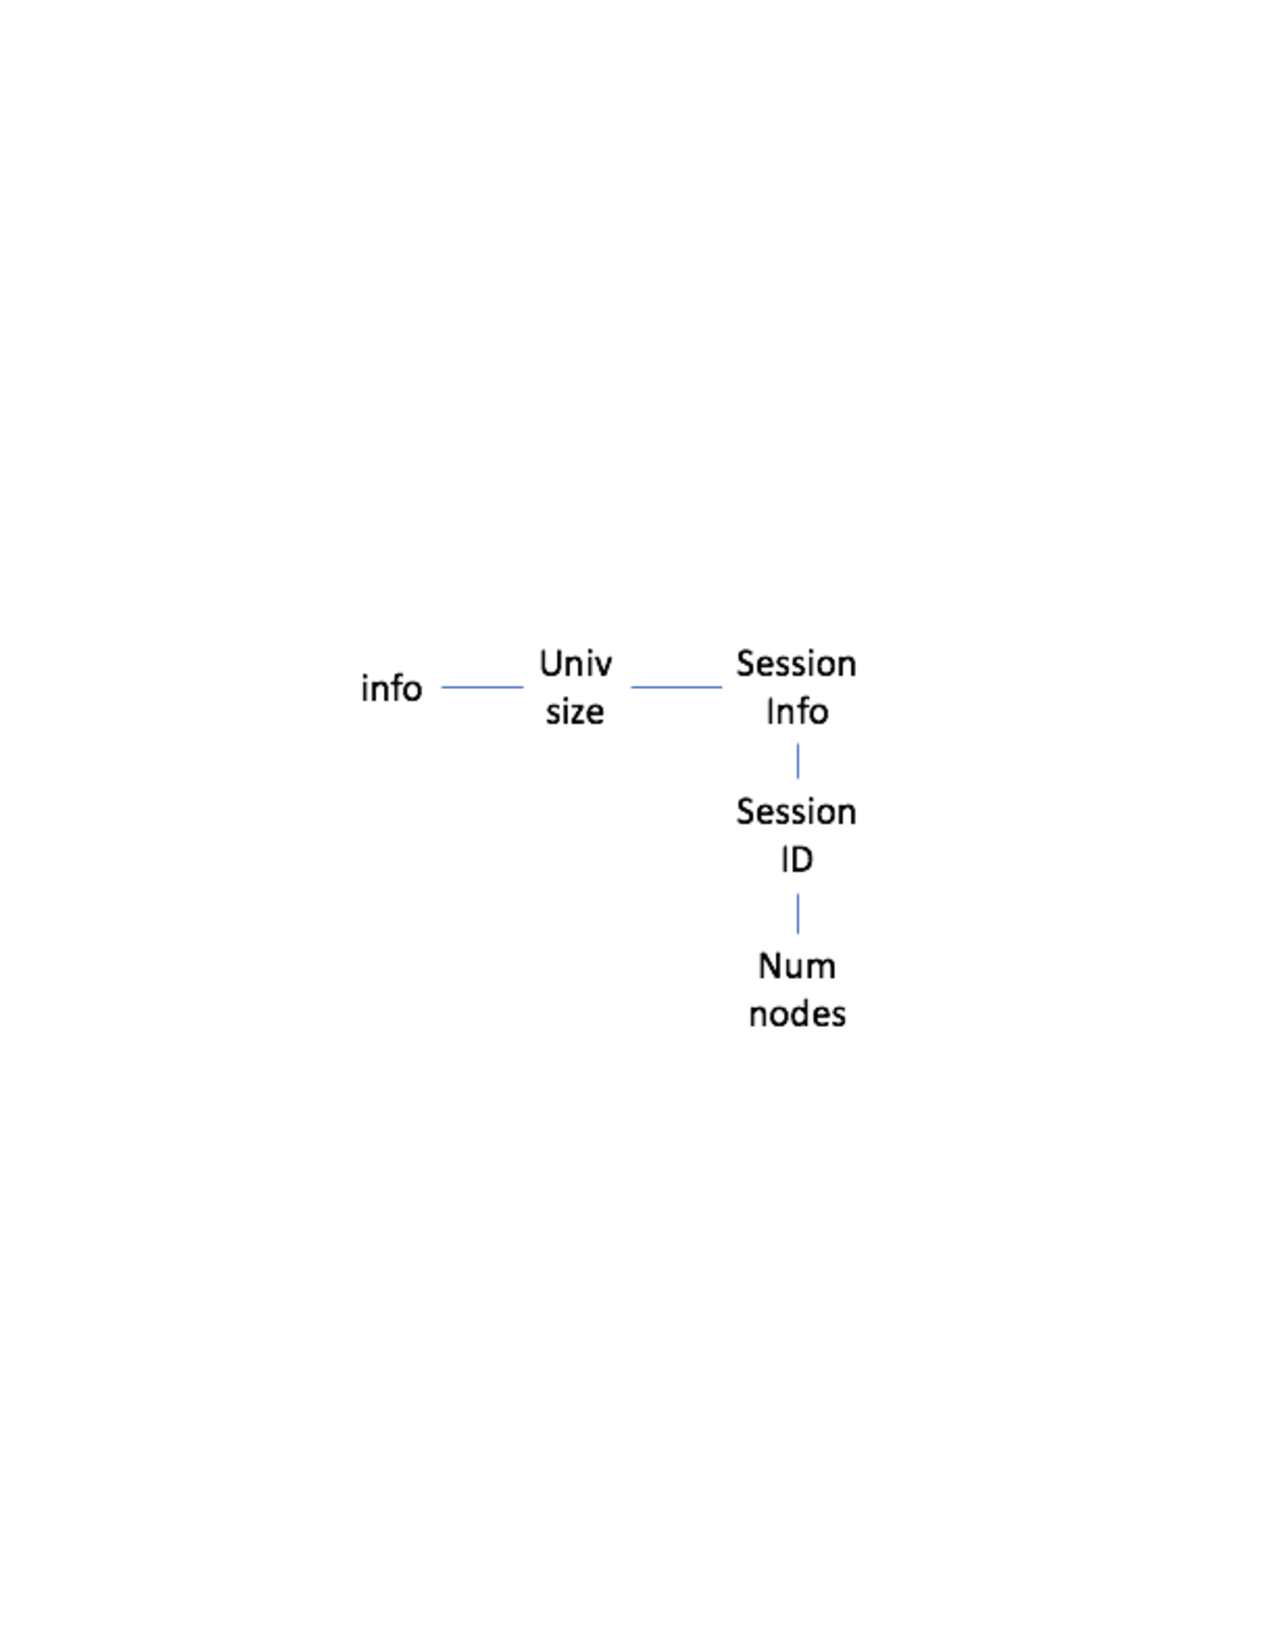
\includegraphics[clip,width=0.3\textwidth]{figs/sessioninfo.pdf}
  \end{center}
  \caption{Session-level information elements}
  \label{fig:sessioninfo}
\end{figure*}
\endgroup


\item Job-level information includes all job-specific values such as \refattr{PMIX_JOB_SIZE}, \refattr{PMIX_JOB_NUM_APPS}, and \refattr{PMIX_JOBID}. Since each invocation of \refapi{PMIx_server_register_nspace} describes a single \refterm{job}, job-specific values can be specified independently - i.e., in their own \refstruct{pmix_info_t} elements of the \refarg{info} array. Alternatively, they can be provided as a \refstruct{pmix_data_array_t} array of \refstruct{pmix_info_t} identified by the \refattr{PMIX_JOB_INFO_ARRAY} attribute - this is \emph{required} in cases where non-specific attributes (e.g., \refattr{PMIX_NODE_MAP}) are passed to describe aspects of the job. Note that since the invocation only involves a single namespace, there is no need to include the \refattr{PMIX_NSPACE} attribute in the array.

Upon conclusion of this step, the \refarg{info} array might look like:

\begingroup
\begin{figure*}[ht!]
  \begin{center}
    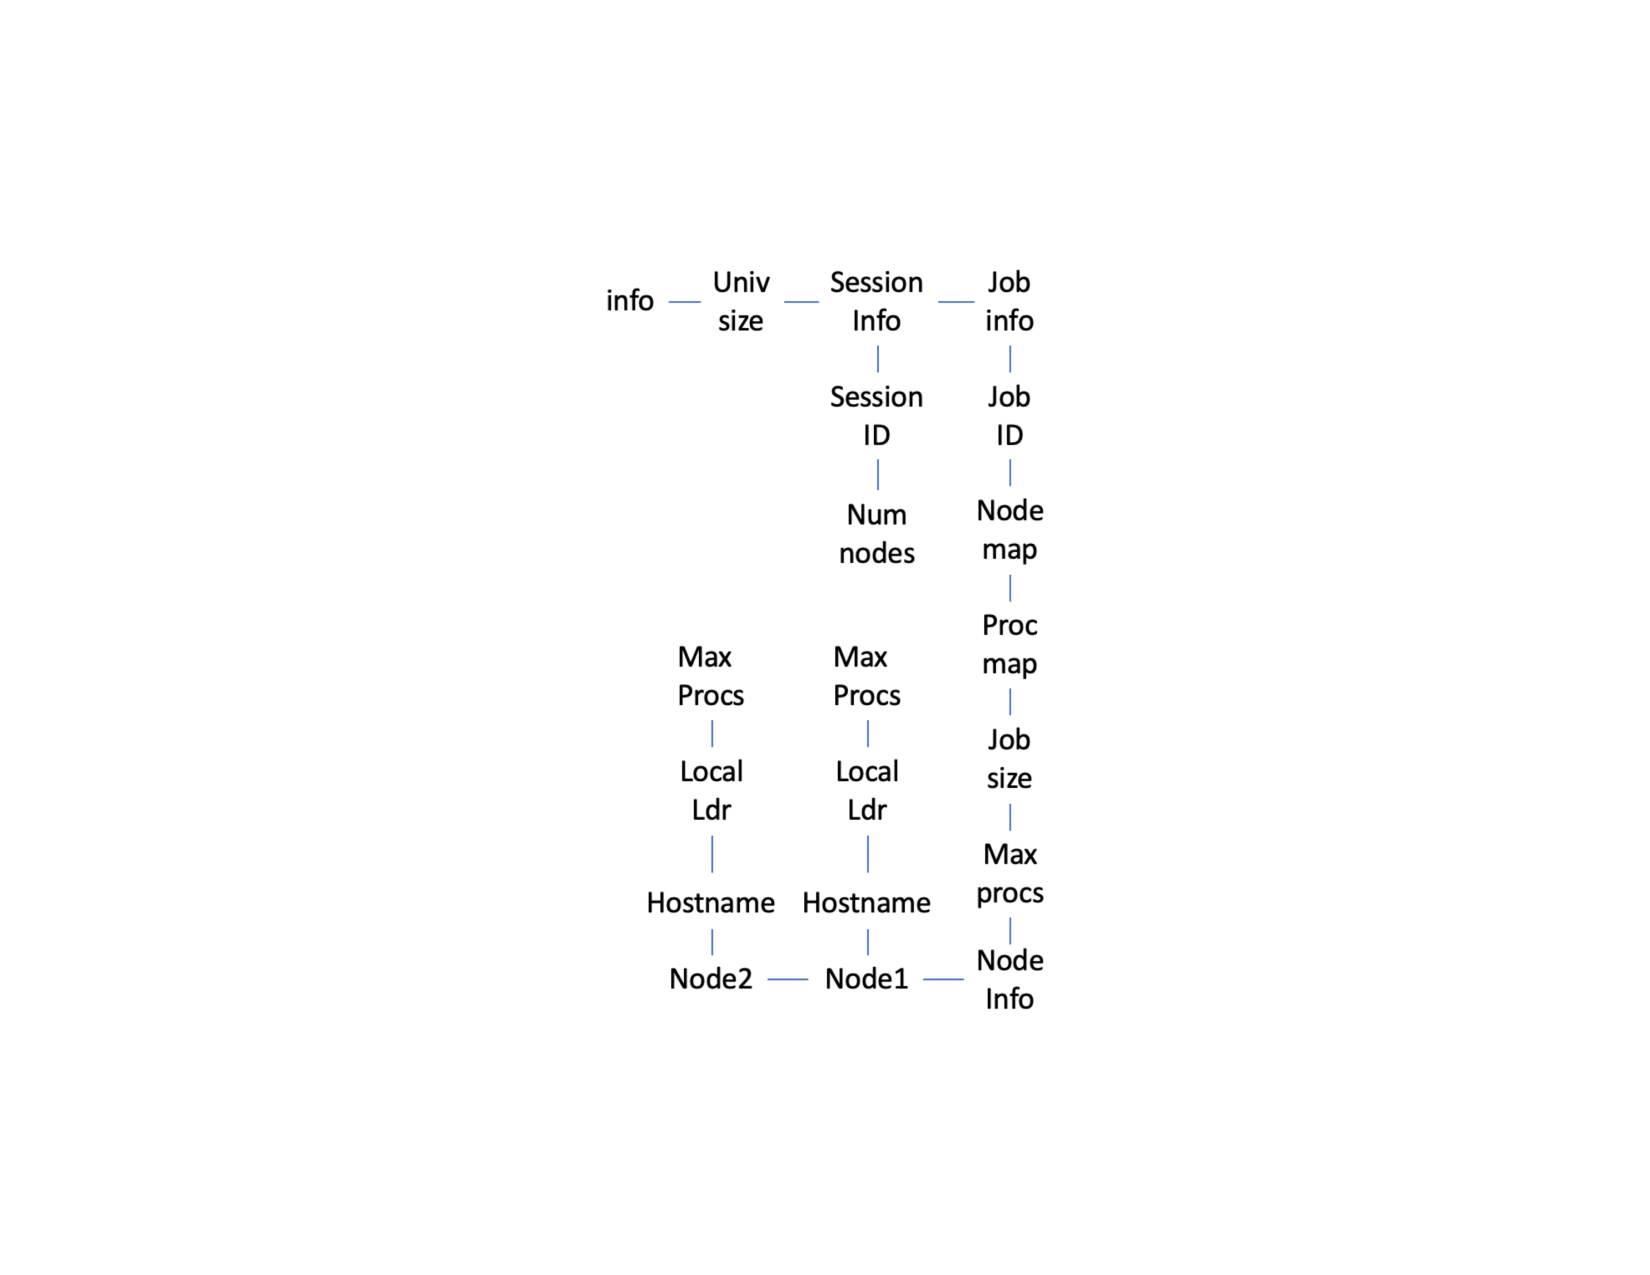
\includegraphics[clip,width=0.4\textwidth]{figs/jobinfo.pdf}
  \end{center}
  \caption{Job-level information elements}
  \label{fig:jobinfo}
\end{figure*}
\endgroup

Note that in this example, \refattr{PMIX_NUM_NODES} is not required as that information is contained in the \refattr{PMIX_NODE_MAP} attribute. Similarly, \refattr{PMIX_JOB_SIZE} is not technically required as that information is contained in the \refattr{PMIX_PROC_MAP} when combined with the corresponding node map - however, there is no issue with including the job size as a separate entry.

The example also illustrates the hierarchical use of the \refattr{PMIX_NODE_INFO_ARRAY} attribute. In this case, we have chosen to pass several job-related values for each node - since those values are non-unique across the job, they must be passed in a node-info container. Note that the choice of what information to pass into the \ac{PMIx} server library versus what information to derive from other values at time of request is left to the host environment. \ac{PMIx} implementors in turn may, if they choose, pre-parse registration data to create expanded views (thus enabling faster response to requests at the expense of memory footprint) or to compress views into tighter representations (thus trading minimized footprint for longer response times).

\item Application-level information includes all application-specific values such as \refattr{PMIX_APP_SIZE} and \refattr{PMIX_APPLDR}. If the \refterm{job} contains only a single \refterm{application}, then the application-specific values can be specified independently - i.e., in their own \refstruct{pmix_info_t} elements of the \refarg{info} array - or as a \refstruct{pmix_data_array_t} array of \refstruct{pmix_info_t} using the \refattr{PMIX_APP_INFO_ARRAY} attribute and identifed by including the \refattr{PMIX_APPNUM} attribute in the array. Use of the array format is  \emph{required} in cases where non-specific attributes (e.g., \refattr{PMIX_NODE_MAP}) are passed to describe aspects of the application.

However, in the case of a job consisting of multiple applications, all application-specific values for each application \emph{must} be provided using the \refattr{PMIX_APP_INFO_ARRAY} format, each identified by its \refattr{PMIX_APPNUM} value.

Upon conclusion of this step, the \refarg{info} array might look like that shown in \ref{fig:appinfo}, assuming there are two applications in the job being registered:

\begingroup
\begin{figure*}[ht!]
  \begin{center}
    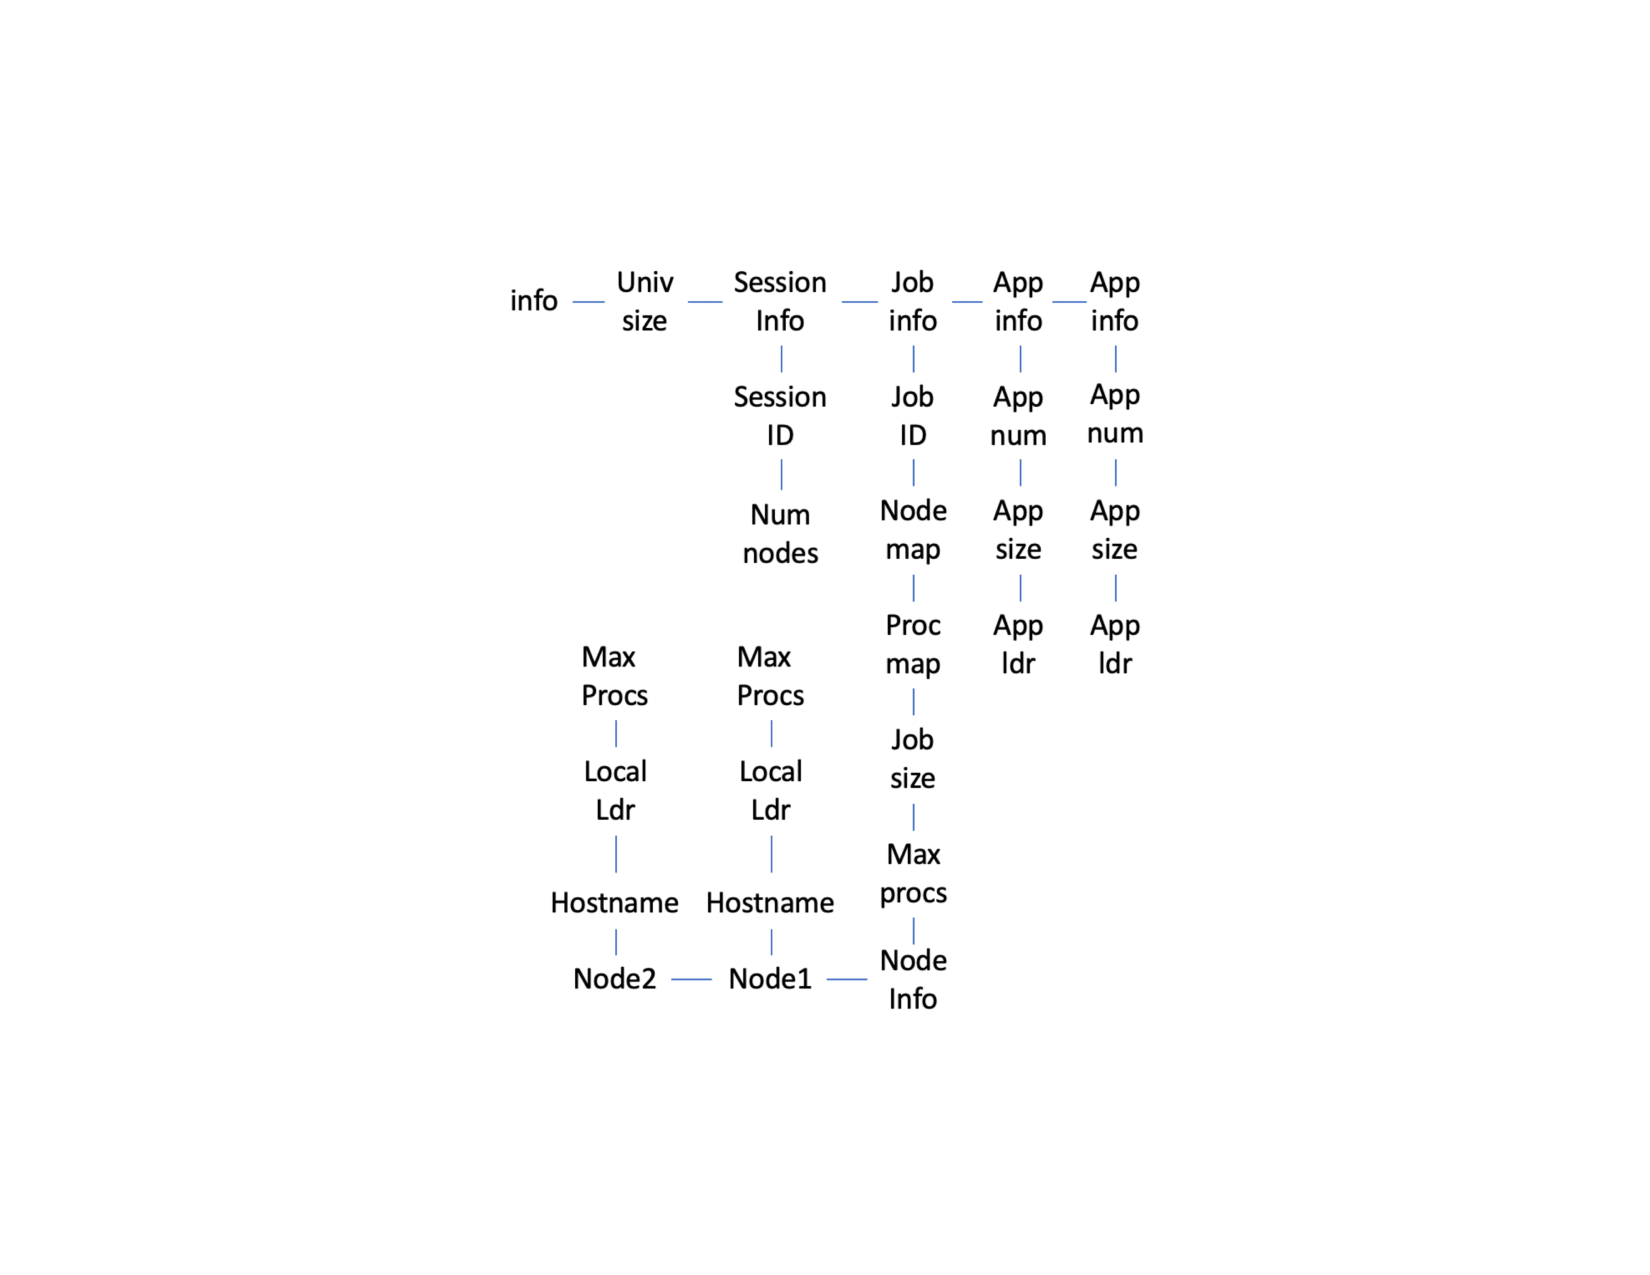
\includegraphics[clip,width=0.5\textwidth]{figs/appinfo.pdf}
  \end{center}
  \caption{Application-level information elements}
  \label{fig:appinfo}
\end{figure*}
\endgroup

\item Process-level information includes an entry for each process in the job being registered, each entry marked with the \refattr{PMIX_PROC_DATA} attribute. The \refterm{rank} of the process \emph{must} be the first entry in the array - this provides efficiency when storing the data. Upon conclusion of this step, the \refarg{info} array might look like the diagram in \ref{fig:procinfo}:

\begingroup
\begin{figure*}[ht!]
  \begin{center}
    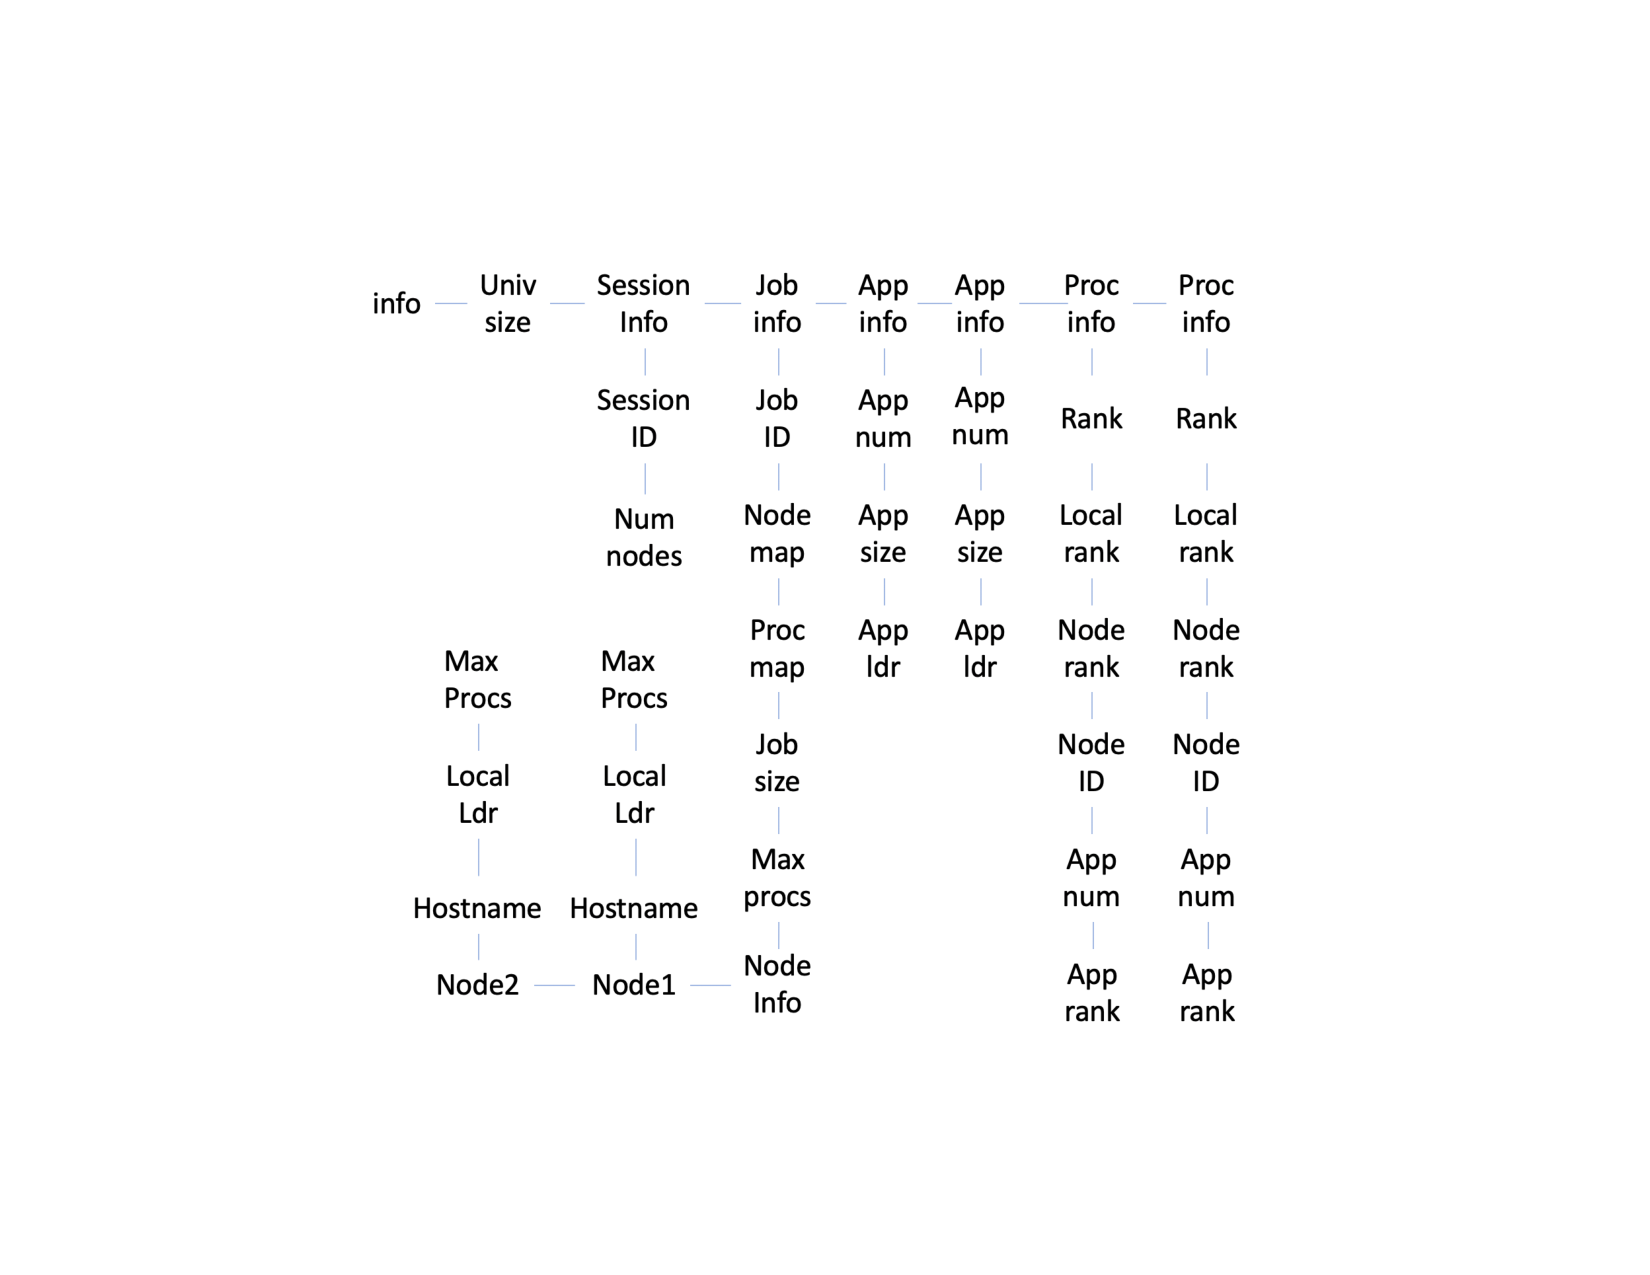
\includegraphics[clip,width=0.5\textwidth]{figs/procinfo.pdf}
  \end{center}
  \caption{Process-level information elements}
  \label{fig:procinfo}
\end{figure*}
\endgroup

\item For purposes of this example, node-level information only includes values describing the local node - i.e., it does not include information about other nodes in the job or session. In many cases, the values included in this level are unique to it and can be specified independently - i.e., in their own \refstruct{pmix_info_t} elements of the \refarg{info} array. Alternatively, they can be provided as a \refstruct{pmix_data_array_t} array of \refstruct{pmix_info_t} using the \refattr{PMIX_NODE_INFO_ARRAY} attribute - this is \emph{required} in cases where non-specific attributes are passed to describe aspects of the node, or where values for multiple nodes are being provided.

The node-level information requires two elements that must be constructed in a manner similar to that used for the node map. The \refattr{PMIX_LOCAL_PEERS} value is computed based on the processes on the local node, filtered to select those from the job being registered, as shown below using the tools provided by \ac{PMIx}:

\cspecificstart
\begin{codepar}
char **ndppn = NULL;
char rank[30];
char *localranks;
size_t m;
pmix_info_t info;

for (m=0; m < mynode->num_procs; m++) {
    /* ignore processes that are not part of the target job */
    if (!PMIX_CHECK_NSPACE(targetjob,mynode->proc[m].nspace)) {
        continue;
    }
    snprintf(rank, 30, "%d", mynode->proc[m].rank);
    PMIX_ARGV_APPEND(&ndppn, rank);
}
/* convert the array into a comma-delimited string of ranks */
localranks = PMIX_ARGV_JOIN(ndppn, ',');
/* release the local array */
PMIX_ARGV_FREE(ndppn);

/* pass the string as the value to the PMIX_LOCAL_PEERS key */
PMIX_INFO_LOAD(&info, PMIX_LOCAL_PEERS, localranks, PMIX_STRING);
/* release the list */
free(localranks);

\end{codepar}
\cspecificend

The \refattr{PMIX_LOCAL_CPUSETS} value is constructed in a similar manner. In the provided example, it is assumed that the \ac{HWLOC} cpuset representation (a comma-delimited string of processor IDs) of the processors assigned to each process has previously been generated and stored on the process description. Thus, the value can be constructed as shown below:

\cspecificstart
\begin{codepar}
char **ndcpus = NULL;
char *localcpus;
size_t m;
pmix_info_t info;

for (m=0; m < mynode->num_procs; m++) {
    /* ignore processes that are not part of the target job */
    if (!PMIX_CHECK_NSPACE(targetjob,mynode->proc[m].nspace)) {
        continue;
    }
    PMIX_ARGV_APPEND(&ndcpus, mynode->proc[m].cpuset);
}
/* convert the array into a colon-delimited string */
localcpus = PMIX_ARGV_JOIN(ndcpus, ':');
/* release the local array */
PMIX_ARGV_FREE(ndcpus);

/* pass the string as the value to the PMIX_LOCAL_CPUSETS key */
PMIX_INFO_LOAD(&info, PMIX_LOCAL_CPUSETS, localcpus, PMIX_STRING);
/* release the list */
free(localcpus);

\end{codepar}
\cspecificend

Note that for efficiency, these two values can be computed at the same time.

\end{itemize}

The final \refarg{info} array might therefore look like the diagram in \ref{fig:nodeinfo}:

\begingroup
\begin{figure*}[ht!]
  \begin{center}
    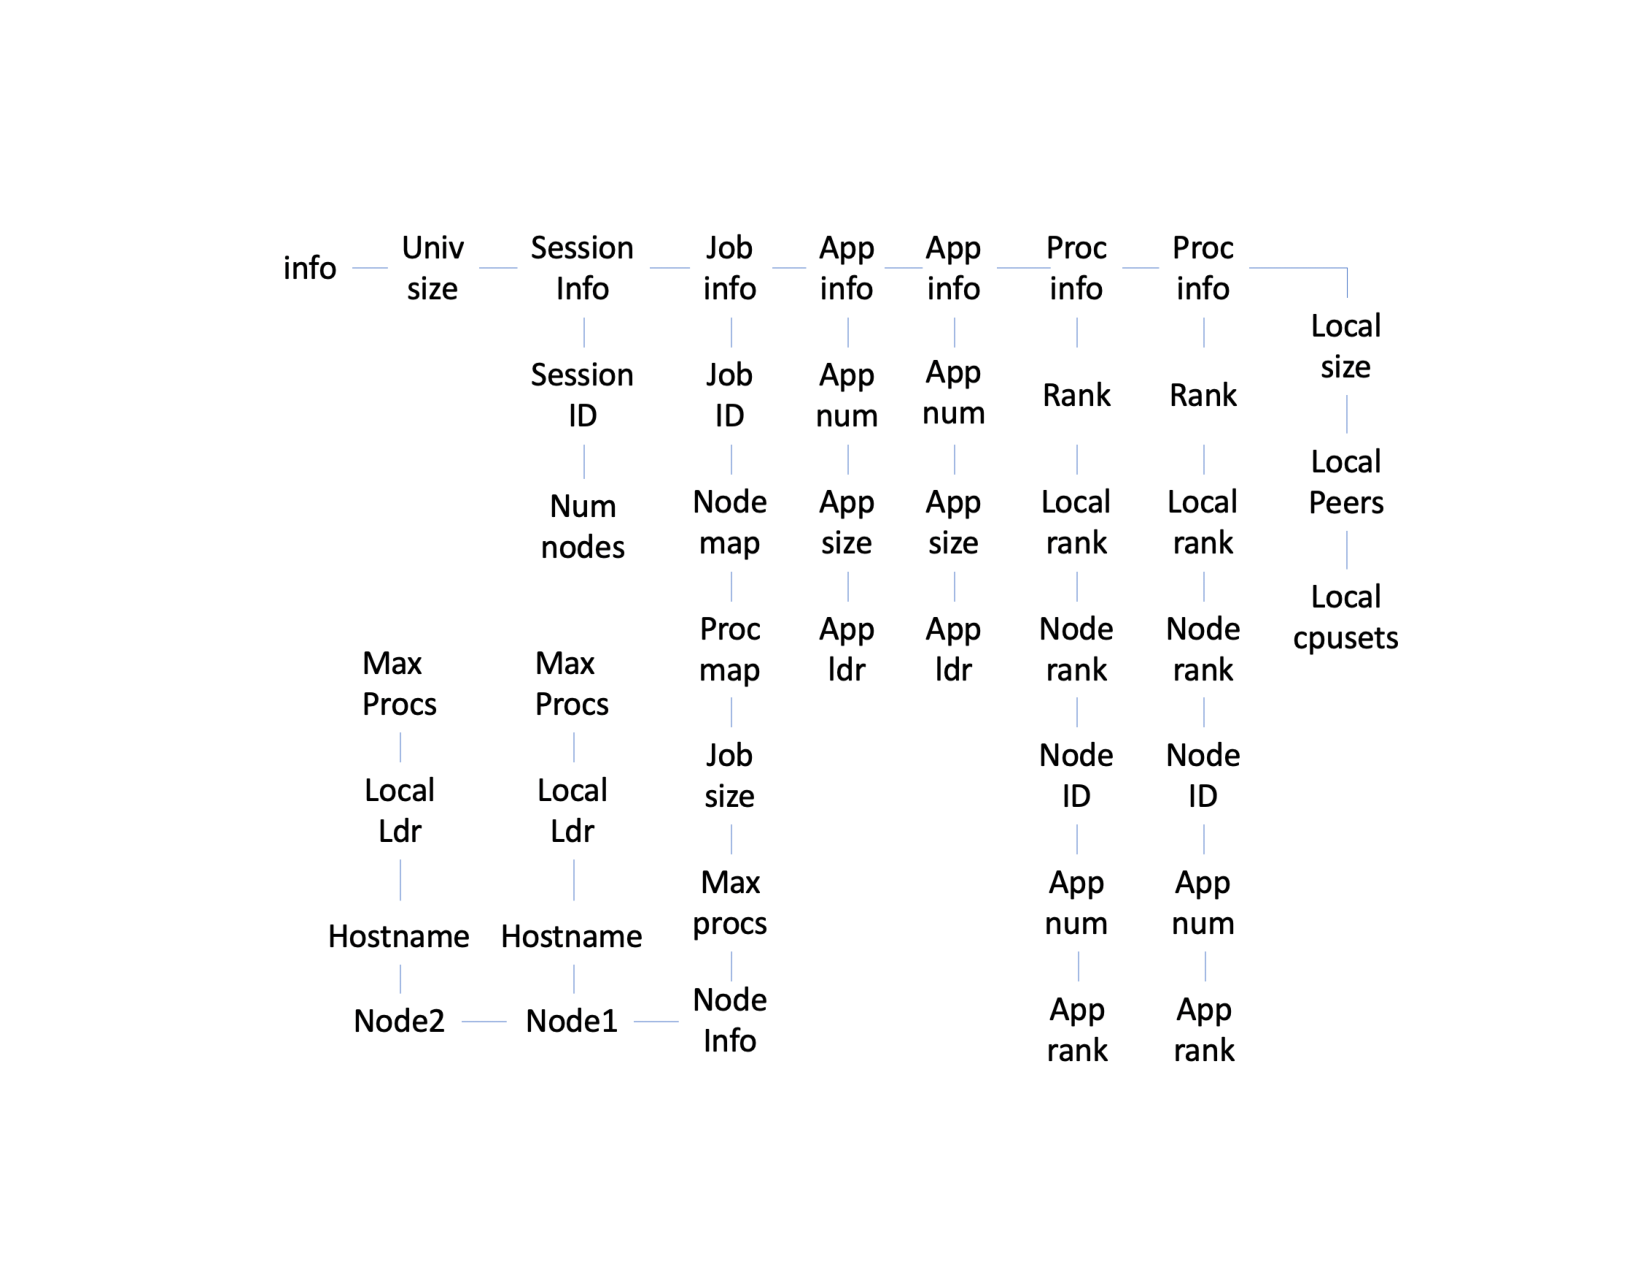
\includegraphics[clip,width=0.8\textwidth]{figs/nodeinfo.pdf}
  \end{center}
  \caption{Final information array}
  \label{fig:nodeinfo}
\end{figure*}
\endgroup


%%%%%%%%%%%
\subsection{\code{PMIx_server_deregister_nspace}}
\declareapi{PMIx_server_deregister_nspace}

%%%%
\summary

Deregister a namespace.

%%%%
\format

\versionMarker{1.0}
\cspecificstart
\begin{codepar}
void PMIx_server_deregister_nspace(const pmix_nspace_t nspace,
                        pmix_op_cbfunc_t cbfunc, void *cbdata)
\end{codepar}
\cspecificend

\begin{arglist}
\argin{nspace}{Namespace (string)}
\argin{cbfunc}{Callback function \refapi{pmix_op_cbfunc_t} (function reference)}
\argin{cbdata}{Data to be passed to the callback function (memory reference)}
\end{arglist}

%%%%
\descr

Deregister the specified \refarg{nspace} and purge all objects relating to it, including any client information from that namespace.
This is intended to support persistent \ac{PMIx} servers by providing an opportunity for the host \ac{RM} to tell the \ac{PMIx} server library to release all memory for a completed job. Note that the library \emph{must not} invoke the callback function prior to returning from the \ac{API}.


%%%%%%%%%%%
\subsection{\code{PMIx_server_register_client}}
\declareapi{PMIx_server_register_client}

%%%%
\summary

Register a client process with the PMIx server library.

%%%%
\format

\versionMarker{1.0}
\cspecificstart
\begin{codepar}
pmix_status_t
PMIx_server_register_client(const pmix_proc_t *proc,
                        uid_t uid, gid_t gid,
                        void *server_object,
                        pmix_op_cbfunc_t cbfunc, void *cbdata)
\end{codepar}
\cspecificend

\begin{arglist}
\argin{proc}{\refstruct{pmix_proc_t} structure (handle)}
\argin{uid}{user id (integer)}
\argin{gid}{group id (integer)}
\argin{server_object}{(memory reference)}
\argin{cbfunc}{Callback function \refapi{pmix_op_cbfunc_t} (function reference)}
\argin{cbdata}{Data to be passed to the callback function (memory reference)}
\end{arglist}

Returns one of the following:

\begin{itemize}
    \item \refconst{PMIX_SUCCESS}, indicating that the request is being processed by the host environment - result will be returned in the provided \refarg{cbfunc}. Note that the library \emph{must not} invoke the callback function prior to returning from the \ac{API}.
    \item \refconst{PMIX_OPERATION_SUCCEEDED}, indicating that the request was immediately processed and returned \textit{success} - the \refarg{cbfunc} will \textit{not} be called
    \item a PMIx error constant indicating either an error in the input or that the request was immediately processed and failed - the \refarg{cbfunc} will \textit{not} be called
\end{itemize}


%%%%
\descr

Register a client process with the PMIx server library.

The host server can also, if it desires, provide an object it wishes to be returned when a server function is called that relates to a specific process.
For example, the host server may have an object that tracks the specific client.
Passing the object to the library allows the library to provide that object to the host server during subsequent calls related to that client, such as a \refapi{pmix_server_client_connected_fn_t} function.  This allows the host server to access the object without performing a lookup based on the client's namespace and rank.

\advicermstart
Host environments are \textit{required} to execute this operation prior to starting the client process.
The expected user ID and group ID of the child process allows the server library to properly authenticate clients as they connect by requiring the two values to match. Accordingly, the detected user and group ID's of the connecting process are not included in the \refapi{pmix_server_client_connected_fn_t} server module function.
\advicermend

\adviceimplstart
For security purposes, the \ac{PMIx} server library should check the user and group ID's of a connecting process against those provided for the declared client process identifier via the \refapi{PMIx_server_register_client} prior to completing the connection.
\adviceimplend

%%%%%%%%%%%
\subsection{\code{PMIx_server_deregister_client}}
\declareapi{PMIx_server_deregister_client}

%%%%
\summary

Deregister a client and purge all data relating to it.

%%%%
\format

\versionMarker{1.0}
\cspecificstart
\begin{codepar}
void
PMIx_server_deregister_client(const pmix_proc_t *proc,
                        pmix_op_cbfunc_t cbfunc, void *cbdata)
\end{codepar}
\cspecificend

\begin{arglist}
\argin{proc}{\refstruct{pmix_proc_t} structure (handle)}
\argin{cbfunc}{Callback function \refapi{pmix_op_cbfunc_t} (function reference)}
\argin{cbdata}{Data to be passed to the callback function (memory reference)}
\end{arglist}


%%%%
\descr

The \refapi{PMIx_server_deregister_nspace} \ac{API} will delete all client information for that namespace. The \ac{PMIx} server library will automatically perform that operation upon disconnect of all local clients.
This \ac{API} is therefore intended primarily for use in exception cases, but can be called in non-exception cases if desired. Note that the library \emph{must not} invoke the callback function prior to returning from the \ac{API}.


%%%%%%%%%%%
\subsection{\code{PMIx_server_setup_fork}}
\declareapi{PMIx_server_setup_fork}

%%%%
\summary

Setup the environment of a child process to be forked by the host.

%%%%
\format

\versionMarker{1.0}
\cspecificstart
\begin{codepar}
pmix_status_t
PMIx_server_setup_fork(const pmix_proc_t *proc,
                        char ***env)
\end{codepar}
\cspecificend

\begin{arglist}
\argin{proc}{\refstruct{pmix_proc_t} structure (handle)}
\argin{env}{Environment array (array of strings)}
\end{arglist}

Returns \refconst{PMIX_SUCCESS} or a negative value corresponding to a PMIx error constant.

%%%%
\descr

Setup the environment of a child process to be forked by the host so it can correctly interact with the PMIx server.

\advicermstart
Host environments are \textit{required} to execute this operation prior to starting the client process.
\advicermend

The \ac{PMIx} client needs some setup information so it can properly connect back to the server.
This function will set appropriate environmental variables for this purpose, and will also provide any environmental variables that were specified in the launch command (e.g., via \refapi{PMIx_Spawn}) plus other values (e.g., variables required to properly initialize the client's fabric library).


%%%%%%%%%%%
\subsection{\code{PMIx_server_dmodex_request}}
\declareapi{PMIx_server_dmodex_request}

%%%%
\summary

Define a function by which the host server can request modex data from the local PMIx server.

%%%%
\format

\versionMarker{1.0}
\cspecificstart
\begin{codepar}
pmix_status_t PMIx_server_dmodex_request(const pmix_proc_t *proc,
                        pmix_dmodex_response_fn_t cbfunc,
                        void *cbdata)
\end{codepar}
\cspecificend

\begin{arglist}
\argin{proc}{\refstruct{pmix_proc_t} structure (handle)}
\argin{cbfunc}{Callback function \refapi{pmix_dmodex_response_fn_t} (function reference)}
\argin{cbdata}{Data to be passed to the callback function (memory reference)}
\end{arglist}

Returns one of the following:

\begin{itemize}
    \item \refconst{PMIX_SUCCESS}, indicating that the request is being processed by the host environment - result will be returned in the provided \refarg{cbfunc}. Note that the library \emph{must not} invoke the callback function prior to returning from the \ac{API}.
    \item a PMIx error constant indicating an error in the input - the \refarg{cbfunc} will \textit{not} be called
\end{itemize}


%%%%
\descr

Define a function by which the host server can request modex data from the local \ac{PMIx} server. Traditional wireup procedures revolve around the per-process posting of data (e.g., location and endpoint information) via the \refapi{PMIx_Put} and \refapi{PMIx_Commit} functions followed by a \refapi{PMIx_Fence} barrier that globally exchanges the posted information. However, the barrier operation represents a signficant time impact at large scale.

\ac{PMIx} supports an alternative wireup method known as \textit{Direct Modex} that replaces the barrier-based exchange of all process-posted information with on-demand fetch of a peer's data. In place of the barrier operation, data posted by each process is cached on the local \ac{PMIx} server. When a process requests the information posted by a particular peer, it first checks the local cache to see if the data is already available. If not, then the request is passed to the local \ac{PMIx} server, which subsequently requests that its \ac{RM} host request the data from the \ac{RM} daemon on the node where the specified peer process is located. Upon receiving the request, the \ac{RM} daemon passes the request into its \ac{PMIx} server library using the \refapi{PMIx_server_dmodex_request} function, receiving the response in the provided \refarg{cbfunc} once the indicated process has posted its information. The \ac{RM} daemon then returns the data to the requesting daemon, who subsequently passes the data to its \ac{PMIx} server library for transfer to the requesting client.

\adviceuserstart
While direct modex allows for faster launch times by eliminating the barrier operation, per-peer retrieval of posted information is less efficient. Optimizations can be implemented - e.g., by returning posted information from all processes on a node upon first request - but in general direct modex remains best suited for sparsely connected applications.
\adviceuserend

%%%%%%%%%%%
\subsection{\code{PMIx_server_setup_application}}
\declareapi{PMIx_server_setup_application}

%%%%
\summary

Provide a function by which the resource manager can request application-specific setup data prior to launch of an application.

%%%%
\format

\versionMarker{2.0}
\cspecificstart
\begin{codepar}
pmix_status_t
PMIx_server_setup_application(const pmix_nspace_t nspace,
                        pmix_info_t info[], size_t ninfo,
                        pmix_setup_application_cbfunc_t cbfunc,
                        void *cbdata)
\end{codepar}
\cspecificend

\begin{arglist}
\argin{nspace}{namespace (string)}
\argin{info}{Array of info structures (array of handles)}
\argin{ninfo}{Number of elements in the \refarg{info} array (integer)}
\argin{cbfunc}{Callback function \refapi{pmix_setup_application_cbfunc_t} (function reference)}
\argin{cbdata}{Data to be passed to the \refarg{cbfunc} callback function (memory reference)}
\end{arglist}

Returns one of the following:

\begin{itemize}
    \item \refconst{PMIX_SUCCESS}, indicating that the request is being processed by the host environment - result will be returned in the provided \refarg{cbfunc}. Note that the library \emph{must not} invoke the callback function prior to returning from the \ac{API}.
    \item a PMIx error constant indicating either an error in the input - the \refarg{cbfunc} will \textit{not} be called
\end{itemize}


\reqattrstart
\ac{PMIx} libraries that support this operation are required to support the following:

\pastePRIAttributeItem{PMIX_SETUP_APP_ENVARS}
\pastePRIAttributeItem{PMIX_SETUP_APP_NONENVARS}
\pastePRIAttributeItem{PMIX_SETUP_APP_ALL}
\pastePRIAttributeItem{PMIX_ALLOC_NETWORK}
\pastePRIAttributeItem{PMIX_ALLOC_NETWORK_ID}
\pastePRIAttributeItem{PMIX_ALLOC_NETWORK_SEC_KEY}
\pastePRIAttributeItem{PMIX_ALLOC_NETWORK_TYPE}
\pastePRIAttributeItem{PMIX_ALLOC_NETWORK_PLANE}
\pastePRIAttributeItem{PMIX_ALLOC_NETWORK_ENDPTS}
\pastePRIAttributeItem{PMIX_ALLOC_NETWORK_ENDPTS_NODE}

\reqattrend

\optattrstart
\ac{PMIx} libraries that support this operation may support the following:

\pastePRIAttributeItem{PMIX_ALLOC_BANDWIDTH}
\pastePRIAttributeItem{PMIX_ALLOC_NETWORK_QOS}
\pastePRIAttributeItem{PMIX_ALLOC_TIME}

\optattrend

%%%%
\descr

Provide a function by which the \ac{RM} can request application-specific setup data (e.g., environmental variables, fabric configuration and security credentials) from supporting \ac{PMIx} server library subsystems prior to initiating launch of an application.

\advicermstart
Host environments are \textit{required} to execute this operation prior to launching an application.
\advicermend

This is defined as a non-blocking operation in case contributing subsystems need to perform some potentially time consuming action (e.g., query a remote service) before responding. The returned data must be distributed by the \ac{RM} and subsequently delivered to the local \ac{PMIx} server on each node where application processes will execute, prior to initiating execution of those processes.

\adviceimplstart
Support for harvesting of environmental variables and providing of local configuration information by the \ac{PMIx} implementation is optional.
\adviceimplend

%%%%%%%%%%%
\subsection{\code{PMIx_server_setup_local_support}}
\declareapi{PMIx_server_setup_local_support}

%%%%
\summary

Provide a function by which the local \ac{PMIx} server can perform any application-specific operations prior to spawning local clients of a given application.

%%%%
\format

\versionMarker{2.0}
\cspecificstart
\begin{codepar}
pmix_status_t
PMIx_server_setup_local_support(const pmix_nspace_t nspace,
                                pmix_info_t info[], size_t ninfo,
                                pmix_op_cbfunc_t cbfunc,
                                void *cbdata);
\end{codepar}
\cspecificend

\begin{arglist}
\argin{nspace}{Namespace (string)}
\argin{info}{Array of info structures (array of handles)}
\argin{ninfo}{Number of elements in the \refarg{info} array (\code{size_t})}
\argin{cbfunc}{Callback function \refapi{pmix_op_cbfunc_t} (function reference)}
\argin{cbdata}{Data to be passed to the callback function (memory reference)}
\end{arglist}

Returns one of the following:

\begin{itemize}
    \item \refconst{PMIX_SUCCESS}, indicating that the request is being processed by the host environment - result will be returned in the provided \refarg{cbfunc}. Note that the library \emph{must not} invoke the callback function prior to returning from the \ac{API}.
    \item \refconst{PMIX_OPERATION_SUCCEEDED}, indicating that the request was immediately processed and returned \textit{success} - the \refarg{cbfunc} will \textit{not} be called
    \item a PMIx error constant indicating either an error in the input or that the request was immediately processed and failed - the \refarg{cbfunc} will \textit{not} be called
\end{itemize}


%%%%
\descr

Provide a function by which the local \ac{PMIx} server can perform any application-specific operations prior to spawning local clients of a given application. For example, a network library might need to setup the local driver for ``instant on'' addressing. The data provided in the \refarg{info} array is the data provided to there host \ac{RM} from the a call to \refapi{PMIx_server_setup_application}.

\advicermstart
Host environments are \textit{required} to execute this operation prior to starting any local application processes from the specified namespace.
\advicermend

%%%%%%%%%%%
\subsection{\code{PMIx_server_IOF_deliver}}
\declareapi{PMIx_server_IOF_deliver}

%%%%
\summary

Provide a function by which the host environment can pass forwarded \ac{IO} to the \ac{PMIx} server library for distribution to its clients.

%%%%
\format

\versionMarker{3.0}
\cspecificstart
\begin{codepar}
pmix_status_t
PMIx_server_IOF_deliver(const pmix_proc_t *source,
                        pmix_iof_channel_t channel,
                        const pmix_byte_object_t *bo,
                        const pmix_info_t info[], size_t ninfo,
                        pmix_op_cbfunc_t cbfunc, void *cbdata);
\end{codepar}
\cspecificend

\begin{arglist}
\argin{source}{Pointer to \refstruct{pmix_proc_t} identifying source of the \ac{IO} (handle)}
\argin{channel}{\ac{IO} channel of the data (\refstruct{pmix_iof_channel_t})}
\argin{bo}{Pointer to \refstruct{pmix_byte_object_t} containing the payload to be delivered (handle)}
\argin{info}{Array of \refstruct{pmix_info_t} metadata describing the data (array of handles)}
\argin{ninfo}{Number of elements in the \refarg{info} array (\code{size_t})}
\argin{cbfunc}{Callback function \refapi{pmix_op_cbfunc_t} (function reference)}
\argin{cbdata}{Data to be passed to the callback function (memory reference)}
\end{arglist}

Returns one of the following:

\begin{itemize}
    \item \refconst{PMIX_SUCCESS}, indicating that the request is being processed by the host environment - result will be returned in the provided \refarg{cbfunc}. Note that the library \emph{must not} invoke the callback function prior to returning from the \ac{API}.
    \item \refconst{PMIX_OPERATION_SUCCEEDED}, indicating that the request was immediately processed and returned \textit{success} - the \refarg{cbfunc} will \textit{not} be called
    \item a PMIx error constant indicating either an error in the input or that the request was immediately processed and failed - the \refarg{cbfunc} will \textit{not} be called
\end{itemize}

%%%%
\descr

Provide a function by which the host environment can pass forwarded \ac{IO} to the \ac{PMIx} server library for distribution to its clients. The \ac{PMIx} server library is responsible for determining which of its clients have actually registered for the provided data and delivering it. The \refarg{cbfunc} callback function will be called once the \ac{PMIx} server library no longer requires access to the provided data.

%%%%%%%%%%%
\subsection{\code{PMIx_server_collect_inventory}}
\declareapi{PMIx_server_collect_inventory}

%%%%
\summary

Collect inventory of resources on a node

%%%%
\format

\versionMarker{3.0}
\cspecificstart
\begin{codepar}
pmix_status_t
PMIx_server_collect_inventory(const pmix_info_t directives[],
                              size_t ndirs,
                              pmix_info_cbfunc_t cbfunc,
                              void *cbdata);
\end{codepar}
\cspecificend

\begin{arglist}
\argin{directives}{Array of \refstruct{pmix_info_t} directing the request (array of handles)}
\argin{ndirs}{Number of elements in the \refarg{directives} array (\code{size_t})}
\argin{cbfunc}{Callback function to return collected data (\refapi{pmix_info_cbfunc_t} function reference)}
\argin{cbdata}{Data to be passed to the callback function (memory reference)}
\end{arglist}

Returns \refconst{PMIX_SUCCESS} or a negative value corresponding to a PMIx error constant. In the event the function returns an error, the \refarg{cbfunc} will \textit{not} be called.

%%%%
\descr

Provide a function by which the host environment can request its \ac{PMIx} server library collect an inventory of local resources. Supported resources depends upon the \ac{PMIx} implementation, but may include the local node topology and network interfaces.

\advicermstart
This is a non-blocking \ac{API} as it may involve somewhat lengthy operations to obtain the requested information. Inventory collection is expected to be a rare event – at system startup and upon command from a system administrator. Inventory updates are expected to initiate a smaller operation involving only the changed information. For example, replacement of a node would generate an event to notify the scheduler with an inventory update without invoking a global inventory operation.
\advicermend

%%%%%%%%%%%
\subsection{\code{PMIx_server_deliver_inventory}}
\declareapi{PMIx_server_deliver_inventory}

%%%%
\summary

Pass collected inventory to the \ac{PMIx} server library for storage

%%%%
\format

\versionMarker{3.0}
\cspecificstart
\begin{codepar}
pmix_status_t
PMIx_server_deliver_inventory(const pmix_info_t info[],
                              size_t ninfo,
                              const pmix_info_t directives[],
                              size_t ndirs,
                              pmix_op_cbfunc_t cbfunc,
                              void *cbdata);
\end{codepar}
\cspecificend

\begin{arglist}
\argin{info}{Array of \refstruct{pmix_info_t} containing the inventory (array of handles)}
\argin{ninfo}{Number of elements in the \refarg{info} array (\code{size_t})}
\argin{directives}{Array of \refstruct{pmix_info_t} directing the request (array of handles)}
\argin{ndirs}{Number of elements in the \refarg{directives} array (\code{size_t})}
\argin{cbfunc}{Callback function \refapi{pmix_op_cbfunc_t} (function reference)}
\argin{cbdata}{Data to be passed to the callback function (memory reference)}
\end{arglist}

Returns one of the following:

\begin{itemize}
    \item \refconst{PMIX_SUCCESS}, indicating that the request is being processed by the host environment - result will be returned in the provided \refarg{cbfunc}. Note that the library \emph{must not} invoke the callback function prior to returning from the \ac{API}.
    \item \refconst{PMIX_OPERATION_SUCCEEDED}, indicating that the request was immediately processed and returned \textit{success} - the \refarg{cbfunc} will \textit{not} be called
    \item a PMIx error constant indicating either an error in the input or that the request was immediately processed and failed - the \refarg{cbfunc} will \textit{not} be called
\end{itemize}


%%%%
\descr

Provide a function by which the host environment can pass inventory information obtained from a node to the \ac{PMIx} server library for storage. Inventory data is subsequently used by the \ac{PMIx} server library for allocations in response to \refapi{PMIx_server_setup_application}, and may be available to the library's host via the \refapi{PMIx_Get} \ac{API} (depending upon \ac{PMIx} implementation). The \refarg{cbfunc} callback function will be called once the \ac{PMIx} server library no longer requires access to the provided data.

%%%%%%%%%%%
\section{Server Function Pointers}

\ac{PMIx} utilizes a "function-shipping" approach to support for implementing the server-side of the protocol. This method allows \acp{RM} to implement the server without being burdened with \ac{PMIx} internal details. When a request is received from the client, the corresponding server function will be called with the information.

Any functions not supported by the \ac{RM} can be indicated by a \code{NULL} for the function pointer. Client calls to such functions will return a \refconst{PMIX_ERR_NOT_SUPPORTED} status.

The host \ac{RM} will provide the function pointers in a \refapi{pmix_server_module_t} structure passed to \refapi{PMIx_server_init}.
That module structure and associated function references are defined in this section.

\advicermstart
For performance purposes, the host server is required to return as quickly as possible from all functions. Execution of
the function is thus to be done asynchronously so as to allow the \ac{PMIx} server support library to handle multiple client requests
as quickly and scalably as possible.

\textit{All} data passed to the host server functions is ``owned'' by the
PMIX server support library and \textit{MUST NOT} be free'd. Data returned
by the host server via callback function is owned by the host
server, which is free to release it upon return from the callback
\advicermend

%%%%%%%%%%%
\subsection{\code{pmix_server_module_t} Module}
\declareapi{pmix_server_module_t}

%%%%
\summary

List of function pointers that a PMIx server passes to \refapi{PMIx_server_init} during startup.

%%%%
\format

\cspecificstart
\begin{codepar}
typedef struct pmix_server_module_3_0_0_t {
    /* v1x interfaces */
    pmix_server_client_connected_fn_t   client_connected;
    pmix_server_client_finalized_fn_t   client_finalized;
    pmix_server_abort_fn_t              abort;
    pmix_server_fencenb_fn_t            fence_nb;
    pmix_server_dmodex_req_fn_t         direct_modex;
    pmix_server_publish_fn_t            publish;
    pmix_server_lookup_fn_t             lookup;
    pmix_server_unpublish_fn_t          unpublish;
    pmix_server_spawn_fn_t              spawn;
    pmix_server_connect_fn_t            connect;
    pmix_server_disconnect_fn_t         disconnect;
    pmix_server_register_events_fn_t    register_events;
    pmix_server_deregister_events_fn_t  deregister_events;
    pmix_server_listener_fn_t           listener;
    /* v2x interfaces */
    pmix_server_notify_event_fn_t       notify_event;
    pmix_server_query_fn_t              query;
    pmix_server_tool_connection_fn_t    tool_connected;
    pmix_server_log_fn_t                log;
    pmix_server_alloc_fn_t              allocate;
    pmix_server_job_control_fn_t        job_control;
    pmix_server_monitor_fn_t            monitor;
    /* v3x interfaces */
    pmix_server_get_cred_fn_t           get_credential;
    pmix_server_validate_cred_fn_t      validate_credential;
    pmix_server_iof_fn_t                iof_pull;
    pmix_server_stdin_fn_t              push_stdin;
} pmix_server_module_t;
\end{codepar}
\cspecificend


%%%%%%%%%%%
\subsection{\code{pmix_server_client_connected_fn_t}}
\declareapi{pmix_server_client_connected_fn_t}

%%%%
\summary

Notify the host server that a client connected to this server.

%%%%
\format

\versionMarker{1.0}
\cspecificstart
\begin{codepar}
typedef pmix_status_t (*pmix_server_client_connected_fn_t)(
                             const pmix_proc_t *proc,
                             void* server_object,
                             pmix_op_cbfunc_t cbfunc,
                             void *cbdata)
\end{codepar}
\cspecificend

\begin{arglist}
\argin{proc}{\refstruct{pmix_proc_t} structure (handle)}
\argin{server_object}{object reference (memory reference)}
\argin{cbfunc}{Callback function \refapi{pmix_op_cbfunc_t} (function reference)}
\argin{cbdata}{Data to be passed to the callback function (memory reference)}
\end{arglist}

Returns one of the following:

\begin{itemize}
    \item \refconst{PMIX_SUCCESS}, indicating that the request is being processed by the host environment - result will be returned in the provided \refarg{cbfunc}. Note that the host \emph{must not} invoke the callback function prior to returning from the \ac{API}.
    \item \refconst{PMIX_OPERATION_SUCCEEDED}, indicating that the request was immediately processed and returned \textit{success} - the \refarg{cbfunc} will \textit{not} be called
    \item a PMIx error constant indicating either an error in the input or that the request was immediately processed and failed - the \refarg{cbfunc} will \textit{not} be called
\end{itemize}

%%%%
\descr

Notify the host environment that a client has called \refapi{PMIx_Init}.
Note that the client will be in a blocked state until the host server executes the callback function, thus allowing the \ac{PMIx} server support library to release
the client.
The server_object parameter will be the value of the server_object parameter passed to
\refapi{PMIx_server_register_client} by the host server when registering the connecting client.  If provided, an implementation of \refapi{pmix_server_client_connected_fn_t}
is only required to
call the callback function designated.  A host server can choose to not be notified when clients connect by setting \refapi{pmix_server_client_connected_fn_t} to \code{NULL}.

It is possible that only a subset of the clients in a namespace call \refapi{PMIx_Init}.   The server's \refapi{pmix_server_client_connected_fn_t} implementation
should not depend on being called once per rank in a namespace or delay calling the callback function until all ranks have connected.
However, if a rank makes any \ac{PMIx} calls, it must first call \refapi{PMIx_Init} and
therefore the server's \refapi{pmix_server_client_connected_fn_t} will be called before any other server functions specific to the rank.

\advicermstart
 This operation is an opportunity for a host environment
 to update the status of the ranks it manages.  It is also a convenient and well defined time to perform initialization necessary to
 support further calls into the server related to that rank.
 \advicermend

%%%%%%%%%%%
\subsection{\code{pmix_server_client_finalized_fn_t}}
\declareapi{pmix_server_client_finalized_fn_t}

%%%%
\summary

Notify the host environment that a client called \refapi{PMIx_Finalize}.

%%%%
\format

\versionMarker{1.0}
\cspecificstart
\begin{codepar}
typedef pmix_status_t (*pmix_server_client_finalized_fn_t)(
                             const pmix_proc_t *proc,
                             void* server_object,
                             pmix_op_cbfunc_t cbfunc,
                             void *cbdata)
\end{codepar}
\cspecificend

\begin{arglist}
\argin{proc}{\refstruct{pmix_proc_t} structure (handle)}
\argin{server_object}{object reference (memory reference)}
\argin{cbfunc}{Callback function \refapi{pmix_op_cbfunc_t} (function reference)}
\argin{cbdata}{Data to be passed to the callback function (memory reference)}
\end{arglist}

Returns one of the following:

\begin{itemize}
    \item \refconst{PMIX_SUCCESS}, indicating that the request is being processed by the host environment - result will be returned in the provided \refarg{cbfunc}. Note that the host \emph{must not} invoke the callback function prior to returning from the \ac{API}.
    \item \refconst{PMIX_OPERATION_SUCCEEDED}, indicating that the request was immediately processed and returned \textit{success} - the \refarg{cbfunc} will \textit{not} be called
    \item a PMIx error constant indicating either an error in the input or that the request was immediately processed and failed - the \refarg{cbfunc} will \textit{not} be called
\end{itemize}

%%%%
\descr

Notify the host environment that a client called \refapi{PMIx_Finalize}.
Note that the client will be in a blocked state until the host server executes the callback function, thus allowing the PMIx server support library to release the client.
The server_object parameter will be the value of the server_object parameter passed to
\refapi{PMIx_server_register_client} by the host server when registering the connecting client.  If provided, an implementation of \refapi{pmix_server_client_finalized_fn_t}
is only required to
call the callback function designated.  A host server can choose to not be notified when clients finalize by setting \refapi{pmix_server_client_finalized_fn_t} to \code{NULL}.

Note that the host server is only being informed that the client has called \refapi{PMIx_Finalize}.  The client might not have exited.  If a client
exits without calling \refapi{PMIx_Finalize}, the server support library will not call the \refapi{pmix_server_client_finalized_fn_t} implementation.

\advicermstart
This operation is an opportunity for a host server
to update the status of the tasks it manages.  It is also a convenient and well defined time to release resources used to support that client.
\advicermend


%%%%%%%%%%%
\subsection{\code{pmix_server_abort_fn_t}}
\declareapi{pmix_server_abort_fn_t}

%%%%
\summary

Notify the host environment that a local client called \refapi{PMIx_Abort}.

%%%%
\format

\versionMarker{1.0}
\cspecificstart
\begin{codepar}
typedef pmix_status_t (*pmix_server_abort_fn_t)(
                             const pmix_proc_t *proc,
                             void *server_object,
                             int status,
                             const char msg[],
                             pmix_proc_t procs[],
                             size_t nprocs,
                             pmix_op_cbfunc_t cbfunc,
                             void *cbdata)
\end{codepar}
\cspecificend


\begin{arglist}
\argin{proc}{\refstruct{pmix_proc_t} structure identifying the process requesting the abort (handle)}
\argin{server_object}{object reference (memory reference)}
\argin{status}{exit status (integer)}
\argin{msg}{exit status message (string)}
\argin{procs}{Array of \refstruct{pmix_proc_t} structures identifying the processes to be terminated (array of handles)}
\argin{nprocs}{Number of elements in the \refarg{procs} array (integer)}
\argin{cbfunc}{Callback function \refapi{pmix_op_cbfunc_t} (function reference)}
\argin{cbdata}{Data to be passed to the callback function (memory reference)}
\end{arglist}

Returns one of the following:

\begin{itemize}
    \item \refconst{PMIX_SUCCESS}, indicating that the request is being processed by the host environment - result will be returned in the provided \refarg{cbfunc}. Note that the host \emph{must not} invoke the callback function prior to returning from the \ac{API}.
    \item \refconst{PMIX_OPERATION_SUCCEEDED}, indicating that the request was immediately processed and returned \textit{success} - the \refarg{cbfunc} will \textit{not} be called
    \item a PMIx error constant indicating either an error in the input or that the request was immediately processed and failed - the \refarg{cbfunc} will \textit{not} be called
\end{itemize}

%%%%
\descr

A local client called \refapi{PMIx_Abort}.
Note that the client will be in a blocked state until the host server executes the callback function, thus allowing the \ac{PMIx} server library to release the client.
The array of \refarg{procs} indicates which processes are to be terminated.
A \code{NULL} indicates that all processes in the client's namespace are to be terminated.


%%%%%%%%%%%
\subsection{\code{pmix_server_fencenb_fn_t}}
\declareapi{pmix_server_fencenb_fn_t}

%%%%
\summary

At least one client called either \refapi{PMIx_Fence} or \refapi{PMIx_Fence_nb}.

%%%%
\format

\versionMarker{1.0}
\cspecificstart
\begin{codepar}
typedef pmix_status_t (*pmix_server_fencenb_fn_t)(
                             const pmix_proc_t procs[],
                             size_t nprocs,
                             const pmix_info_t info[],
                             size_t ninfo,
                             char *data, size_t ndata,
                             pmix_modex_cbfunc_t cbfunc,
                             void *cbdata)
\end{codepar}
\cspecificend

\begin{arglist}
\argin{procs}{Array of \refstruct{pmix_proc_t} structures identifying operation participants(array of handles)}
\argin{nprocs}{Number of elements in the \refarg{procs} array (integer)}
\argin{info}{Array of info structures (array of handles)}
\argin{ninfo}{Number of elements in the \refarg{info} array (integer)}
\argin{data}{(string)}
\argin{ndata}{(integer)}
\argin{cbfunc}{Callback function \refapi{pmix_modex_cbfunc_t} (function reference)}
\argin{cbdata}{Data to be passed to the callback function (memory reference)}
\end{arglist}

Returns one of the following:

\begin{itemize}
    \item \refconst{PMIX_SUCCESS}, indicating that the request is being processed by the host environment - result will be returned in the provided \refarg{cbfunc}. Note that the host \emph{must not} invoke the callback function prior to returning from the \ac{API}.
    \item \refconst{PMIX_OPERATION_SUCCEEDED}, indicating that the request was immediately processed and returned \textit{success} - the \refarg{cbfunc} will \textit{not} be called
    \item a PMIx error constant indicating either an error in the input or that the request was immediately processed and failed - the \refarg{cbfunc} will \textit{not} be called
\end{itemize}

\reqattrstart
\ac{PMIx} libraries are required to pass any provided attributes to the host environment for processing.

\divider

The following attributes are required to be supported by all host environments:

\pastePRRTEAttributeItem{PMIX_COLLECT_DATA}

\reqattrend

\optattrstart
The following attributes are optional for host environments:

\pastePRRTEAttributeItem{PMIX_TIMEOUT}
\pasteAttributeItem{PMIX_COLLECTIVE_ALGO}
\pasteAttributeItem{PMIX_COLLECTIVE_ALGO_REQD}

\optattrend

\advicermstart
Host environment are \textit{required} to return \refconst{PMIX_ERR_NOT_SUPPORTED} if passed an attributed marked as \refconst{PMIX_INFO_REQD} that they do not support, even if support for that attribute is optional.
\advicermend

%%%%
\descr

All local clients in the provided array of \refarg{procs} called either \refapi{PMIx_Fence} or \refapi{PMIx_Fence_nb}.
In either case, the host server will be called via a non-blocking function to execute the specified operation once all participating local processes have contributed.
All processes in the specified \refarg{procs} array are required to participate in the \refapi{PMIx_Fence}/\refapi{PMIx_Fence_nb} operation.
The callback is to be executed once every daemon hosting at least one participant has called the host server's \refapi{pmix_server_fencenb_fn_t} function.

\adviceimplstart
The \ac{PMIx} server library is required to aggregate participation by local clients, passing the request to the host environment once all local participants have executed the \ac{API}.
\adviceimplend

\advicermstart
The host will receive a single call for each collective operation. It is the responsibility of the host to identify the nodes containing participating processes, execute the collective across all participating nodes, and notify the local \ac{PMIx} server library upon completion of the global collective.
\advicermend

The provided data is to be collectively shared with all \ac{PMIx} servers involved in the fence operation, and returned in the modex \refarg{cbfunc}.
A \code{NULL} data value indicates that the local processes had no data to contribute.

The array of \refarg{info} structs is used to pass user-requested options to the server.
This can include directives as to the algorithm to be used to execute the fence operation.
The directives are optional \emph{unless} the \refconst{PMIX_INFO_REQD} flag has been set - in such cases, the host \ac{RM} is required to return an error if the directive cannot be met.


%%%%%%%%%%%
\subsection{\code{pmix_server_dmodex_req_fn_t}}
\declareapi{pmix_server_dmodex_req_fn_t}

%%%%
\summary

Used by the PMIx server to request its local host contact the \ac{PMIx} server on the remote node that hosts the specified proc to obtain and return a direct modex blob for that proc.

%%%%
\format

\versionMarker{1.0}
\cspecificstart
\begin{codepar}
typedef pmix_status_t (*pmix_server_dmodex_req_fn_t)(
                             const pmix_proc_t *proc,
                             const pmix_info_t info[],
                             size_t ninfo,
                             pmix_modex_cbfunc_t cbfunc,
                             void *cbdata)
\end{codepar}
\cspecificend

\begin{arglist}
\argin{proc}{\refstruct{pmix_proc_t} structure identifying the process whose data is being requested (handle)}
\argin{info}{Array of info structures (array of handles)}
\argin{ninfo}{Number of elements in the \refarg{info} array (integer)}
\argin{cbfunc}{Callback function \refapi{pmix_modex_cbfunc_t} (function reference)}
\argin{cbdata}{Data to be passed to the callback function (memory reference)}
\end{arglist}

Returns one of the following:

\begin{itemize}
    \item \refconst{PMIX_SUCCESS}, indicating that the request is being processed by the host environment - result will be returned in the provided \refarg{cbfunc}. Note that the host \emph{must not} invoke the callback function prior to returning from the \ac{API}.
    \item a PMIx error constant indicating either an error in the input or that the request was immediately processed and failed - the \refarg{cbfunc} will \textit{not} be called
\end{itemize}

\reqattrstart
\ac{PMIx} libraries are required to pass any provided attributes to the host environment for processing.
\reqattrend

\optattrstart
The following attributes are optional for host environments that support this operation:

\pastePRRTEAttributeItem{PMIX_TIMEOUT}

\optattrend

%%%%
\descr

Used by the \ac{PMIx} server to request its local host contact the \ac{PMIx} server on the remote node that hosts the specified proc to obtain and return any information that process posted via calls to \refapi{PMIx_Put} and \refapi{PMIx_Commit}.

The array of \refarg{info} structs is used to pass user-requested options to the server.
This can include a timeout to preclude an indefinite wait for data that may never become available.
The directives are optional \emph{unless} the \emph{mandatory} flag has been set - in such cases, the host \ac{RM} is required to return an error if the directive cannot be met.


%%%%%%%%%%%
\subsection{\code{pmix_server_publish_fn_t}}
\declareapi{pmix_server_publish_fn_t}

%%%%
\summary

Publish data per the PMIx API specification.

%%%%
\format

\versionMarker{1.0}
\cspecificstart
\begin{codepar}
typedef pmix_status_t (*pmix_server_publish_fn_t)(
                             const pmix_proc_t *proc,
                             const pmix_info_t info[],
                             size_t ninfo,
                             pmix_op_cbfunc_t cbfunc,
                             void *cbdata)
\end{codepar}
\cspecificend

\begin{arglist}
\argin{proc}{\refstruct{pmix_proc_t} structure of the process publishing the data (handle)}
\argin{info}{Array of info structures (array of handles)}
\argin{ninfo}{Number of elements in the \refarg{info} array (integer)}
\argin{cbfunc}{Callback function \refapi{pmix_op_cbfunc_t} (function reference)}
\argin{cbdata}{Data to be passed to the callback function (memory reference)}
\end{arglist}

Returns one of the following:

\begin{itemize}
    \item \refconst{PMIX_SUCCESS}, indicating that the request is being processed by the host environment - result will be returned in the provided \refarg{cbfunc}. Note that the host \emph{must not} invoke the callback function prior to returning from the \ac{API}.
    \item \refconst{PMIX_OPERATION_SUCCEEDED}, indicating that the request was immediately processed and returned \textit{success} - the \refarg{cbfunc} will \textit{not} be called
    \item a PMIx error constant indicating either an error in the input or that the request was immediately processed and failed - the \refarg{cbfunc} will \textit{not} be called
\end{itemize}

\reqattrstart
\ac{PMIx} libraries are required to pass any provided attributes to the host environment for processing. In addition, the following attributes are required to be included in the passed \refarg{info} array:

\pastePRIAttributeItem{PMIX_USERID}
\pastePRIAttributeItem{PMIX_GRPID}

\divider

Host environments that implement this entry point are required to support the following attributes:

\pastePRRTEAttributeItem{PMIX_RANGE}
\pastePRRTEAttributeItem{PMIX_PERSISTENCE}

\reqattrend

\optattrstart
The following attributes are optional for host environments that support this operation:

\pasteAttributeItem{PMIX_TIMEOUT}

\optattrend

%%%%
\descr

Publish data per the \refapi{PMIx_Publish} specification.
The callback is to be executed upon completion of the operation.
The default data range is left to the host environment, but expected to be \refconst{PMIX_SESSION}, and the default persistence \refconst{PMIX_PERSIST_SESSION} or their equivalent.
These values can be specified by including the respective attributed in the \refarg{info} array.

The persistence indicates how long the server should retain the data.

\advicermstart
The host environment is not required to guarantee support for any specific range - i.e., the environment does not need to return an error if the data store doesn't support a specified range so long as it is covered by some internally defined range.
However, the server must return an error (a) if the key is duplicative within the storage range, and (b) if the server does not allow overwriting of published info by the original publisher - it is left to the discretion of the host environment to allow info-key-based flags to modify this behavior.

The \refattr{PMIX_USERID} and \refattr{PMIX_GRPID} of the publishing process will be provided to support authorization-based access to published information and must be returned on any subsequent lookup request.
\advicermend

%%%%%%%%%%%
\subsection{\code{pmix_server_lookup_fn_t}}
\declareapi{pmix_server_lookup_fn_t}

%%%%
\summary

Lookup published data.

%%%%
\format

\versionMarker{1.0}
\cspecificstart
\begin{codepar}
typedef pmix_status_t (*pmix_server_lookup_fn_t)(
                             const pmix_proc_t *proc,
                             char **keys,
                             const pmix_info_t info[],
                             size_t ninfo,
                             pmix_lookup_cbfunc_t cbfunc,
                             void *cbdata)
\end{codepar}
\cspecificend

\begin{arglist}
\argin{proc}{\refstruct{pmix_proc_t} structure of the process seeking the data (handle)}
\argin{keys}{(array of strings)}
\argin{info}{Array of info structures (array of handles)}
\argin{ninfo}{Number of elements in the \refarg{info} array (integer)}
\argin{cbfunc}{Callback function \refapi{pmix_lookup_cbfunc_t} (function reference)}
\argin{cbdata}{Data to be passed to the callback function (memory reference)}
\end{arglist}

Returns one of the following:

\begin{itemize}
    \item \refconst{PMIX_SUCCESS}, indicating that the request is being processed by the host environment - result will be returned in the provided \refarg{cbfunc}. Note that the host \emph{must not} invoke the callback function prior to returning from the \ac{API}.
    \item \refconst{PMIX_OPERATION_SUCCEEDED}, indicating that the request was immediately processed and returned \textit{success} - the \refarg{cbfunc} will \textit{not} be called
    \item a PMIx error constant indicating either an error in the input or that the request was immediately processed and failed - the \refarg{cbfunc} will \textit{not} be called
\end{itemize}

\reqattrstart
\ac{PMIx} libraries are required to pass any provided attributes to the host environment for processing. In addition, the following attributes are required to be included in the passed \refarg{info} array:

\pastePRIAttributeItem{PMIX_USERID}
\pastePRIAttributeItem{PMIX_GRPID}

\divider

Host environments that implement this entry point are required to support the following attributes:

\pastePRRTEAttributeItem{PMIX_RANGE}
\pastePRRTEAttributeItem{PMIX_WAIT}

\reqattrend

\optattrstart
The following attributes are optional for host environments that support this operation:

\pasteAttributeItem{PMIX_TIMEOUT}

\optattrend


%%%%
\descr

Lookup published data.
The host server will be passed a \code{NULL}-terminated array of string keys identifying the data being requested.

The array of \refarg{info} structs is used to pass user-requested options to the server. The default data range is left to the host environment, but expected to be \refconst{PMIX_SESSION}.
This can include a wait flag to indicate that the server should wait for all data to become available before executing the callback function, or should immediately callback with whatever data is available.
In addition, a timeout can be specified on the wait to preclude an indefinite wait for data that may never be published.

\advicermstart
The \refattr{PMIX_USERID} and \refattr{PMIX_GRPID} of the requesting process will be provided to support authorization-based access to published information. The host environment is not required to guarantee support for any specific range - i.e., the environment does not need to return an error if the data store doesn't support a specified range so long as it is covered by some internally defined range.
\advicermend

%%%%%%%%%%%
\subsection{\code{pmix_server_unpublish_fn_t}}
\declareapi{pmix_server_unpublish_fn_t}

%%%%
\summary

Delete data from the data store.

%%%%
\format

\versionMarker{1.0}
\cspecificstart
\begin{codepar}
typedef pmix_status_t (*pmix_server_unpublish_fn_t)(
                             const pmix_proc_t *proc,
                             char **keys,
                             const pmix_info_t info[],
                             size_t ninfo,
                             pmix_op_cbfunc_t cbfunc,
                             void *cbdata)
\end{codepar}
\cspecificend

\begin{arglist}
\argin{proc}{\refstruct{pmix_proc_t} structure identifying the process making the request (handle)}
\argin{keys}{(array of strings)}
\argin{info}{Array of info structures (array of handles)}
\argin{ninfo}{Number of elements in the \refarg{info} array (integer)}
\argin{cbfunc}{Callback function \refapi{pmix_op_cbfunc_t} (function reference)}
\argin{cbdata}{Data to be passed to the callback function (memory reference)}
\end{arglist}

Returns one of the following:

\begin{itemize}
    \item \refconst{PMIX_SUCCESS}, indicating that the request is being processed by the host environment - result will be returned in the provided \refarg{cbfunc}. Note that the host \emph{must not} invoke the callback function prior to returning from the \ac{API}.
    \item \refconst{PMIX_OPERATION_SUCCEEDED}, indicating that the request was immediately processed and returned \textit{success} - the \refarg{cbfunc} will \textit{not} be called
    \item a PMIx error constant indicating either an error in the input or that the request was immediately processed and failed - the \refarg{cbfunc} will \textit{not} be called
\end{itemize}

\reqattrstart
\ac{PMIx} libraries are required to pass any provided attributes to the host environment for processing. In addition, the following attributes are required to be included in the passed \refarg{info} array:

\pastePRIAttributeItem{PMIX_USERID}
\pastePRIAttributeItem{PMIX_GRPID}

\divider

Host environments that implement this entry point are required to support the following attributes:

\pastePRRTEAttributeItem{PMIX_RANGE}

\reqattrend

\optattrstart
The following attributes are optional for host environments that support this operation:

\pasteAttributeItem{PMIX_TIMEOUT}

\optattrend

%%%%
\descr

Delete data from the data store.
The host server will be passed a \code{NULL}-terminated array of string keys, plus potential directives such as the data range within which the keys should be deleted. The default data range is left to the host environment, but expected to be \refconst{PMIX_SESSION}.
The callback is to be executed upon completion of the delete procedure.

\advicermstart
The \refattr{PMIX_USERID} and \refattr{PMIX_GRPID} of the requesting process will be provided to support authorization-based access to published information. The host environment is not required to guarantee support for any specific range - i.e., the environment does not need to return an error if the data store doesn't support a specified range so long as it is covered by some internally defined range.
\advicermend


%%%%%%%%%%%
\subsection{\code{pmix_server_spawn_fn_t}}
\declareapi{pmix_server_spawn_fn_t}

%%%%
\summary

Spawn a set of applications/processes as per the \refapi{PMIx_Spawn} API.

%%%%
\format

\versionMarker{1.0}
\cspecificstart
\begin{codepar}
typedef pmix_status_t (*pmix_server_spawn_fn_t)(
                             const pmix_proc_t *proc,
                             const pmix_info_t job_info[],
                             size_t ninfo,
                             const pmix_app_t apps[],
                             size_t napps,
                             pmix_spawn_cbfunc_t cbfunc,
                             void *cbdata)
\end{codepar}
\cspecificend

\begin{arglist}
\argin{proc}{\refstruct{pmix_proc_t} structure of the process making the request (handle)}
\argin{job_info}{Array of info structures (array of handles)}
\argin{ninfo}{Number of elements in the \refarg{jobinfo} array (integer)}
\argin{apps}{Array of \refstruct{pmix_app_t} structures (array of handles)}
\argin{napps}{Number of elements in the \refarg{apps} array (integer)}
\argin{cbfunc}{Callback function \refapi{pmix_spawn_cbfunc_t} (function reference)}
\argin{cbdata}{Data to be passed to the callback function (memory reference)}
\end{arglist}

Returns one of the following:

\begin{itemize}
    \item \refconst{PMIX_SUCCESS}, indicating that the request is being processed by the host environment - result will be returned in the provided \refarg{cbfunc}. Note that the host \emph{must not} invoke the callback function prior to returning from the \ac{API}.
    \item \refconst{PMIX_OPERATION_SUCCEEDED}, indicating that the request was immediately processed and returned \textit{success} - the \refarg{cbfunc} will \textit{not} be called
    \item a PMIx error constant indicating either an error in the input or that the request was immediately processed and failed - the \refarg{cbfunc} will \textit{not} be called
\end{itemize}

\reqattrstart
\ac{PMIx} libraries are required to pass any provided attributes to the host environment for processing. In addition, the following attributes are required to be included in the passed \refarg{info} array:

\pastePRIAttributeItem{PMIX_USERID}
\pastePRIAttributeItem{PMIX_GRPID}

\divider

Host environments that provide this module entry point are required to pass the \refattr{PMIX_SPAWNED} and \refattr{PMIX_PARENT_ID} attributes to all \ac{PMIx} servers launching new child processes so those values can be returned to clients upon connection to the \ac{PMIx} server. In addition, they are required to support the following attributes when present in either the \refarg{job_info} or the \textit{info} array of an element of the \refarg{apps} array:

\pastePRRTEAttributeItem{PMIX_WDIR}
\pastePRRTEAttributeItem{PMIX_SET_SESSION_CWD}
\pastePRRTEAttributeItem{PMIX_PREFIX}
\pastePRRTEAttributeItem{PMIX_HOST}
\pastePRRTEAttributeItem{PMIX_HOSTFILE}

\reqattrend

\optattrstart
The following attributes are optional for host environments that support this operation:

\pastePRRTEAttributeItem{PMIX_ADD_HOSTFILE}
\pastePRRTEAttributeItem{PMIX_ADD_HOST}
\pastePRRTEAttributeItem{PMIX_PRELOAD_BIN}
\pastePRRTEAttributeItem{PMIX_PRELOAD_FILES}
\pastePRRTEAttributeItem{PMIX_PERSONALITY}
\pastePRRTEAttributeItem{PMIX_MAPPER}
\pastePRRTEAttributeItem{PMIX_DISPLAY_MAP}
\pastePRRTEAttributeItem{PMIX_PPR}
\pastePRRTEAttributeItem{PMIX_MAPBY}
\pastePRRTEAttributeItem{PMIX_RANKBY}
\pastePRRTEAttributeItem{PMIX_BINDTO}
\pastePRRTEAttributeItem{PMIX_NON_PMI}
\pastePRRTEAttributeItem{PMIX_STDIN_TGT}
\pastePRRTEAttributeItem{PMIX_FWD_STDIN}
\pastePRRTEAttributeItem{PMIX_FWD_STDOUT}
\pastePRRTEAttributeItem{PMIX_FWD_STDERR}
\pastePRRTEAttributeItem{PMIX_DEBUGGER_DAEMONS}
\pastePRRTEAttributeItem{PMIX_TAG_OUTPUT}
\pastePRRTEAttributeItem{PMIX_TIMESTAMP_OUTPUT}
\pastePRRTEAttributeItem{PMIX_MERGE_STDERR_STDOUT}
\pastePRRTEAttributeItem{PMIX_OUTPUT_TO_FILE}
\pastePRRTEAttributeItem{PMIX_INDEX_ARGV}
\pastePRRTEAttributeItem{PMIX_CPUS_PER_PROC}
\pastePRRTEAttributeItem{PMIX_NO_PROCS_ON_HEAD}
\pastePRRTEAttributeItem{PMIX_NO_OVERSUBSCRIBE}
\pastePRRTEAttributeItem{PMIX_REPORT_BINDINGS}
\pastePRRTEAttributeItem{PMIX_CPU_LIST}
\pastePRRTEAttributeItem{PMIX_JOB_RECOVERABLE}
\pastePRRTEAttributeItem{PMIX_JOB_CONTINUOUS}
\pastePRRTEAttributeItem{PMIX_MAX_RESTARTS}
\pasteAttributeItem{PMIX_TIMEOUT}

\optattrend

%%%%
\descr

Spawn a set of applications/processes as per the \refapi{PMIx_Spawn} API.
Note that applications are not required to be \ac{MPI} or any other programming model.
Thus, the host server cannot make any assumptions as to their required support.
The callback function is to be executed once all processes have been started.
An error in starting any application or process in this request shall cause all applications and processes in the request to be terminated, and an error returned to the originating caller.

Note that a timeout can be specified in the job_info array to indicate that failure to start the requested job within the given time should result in termination to avoid hangs.


%%%%%%%%%%%
\subsection{\code{pmix_server_connect_fn_t}}
\declareapi{pmix_server_connect_fn_t}

%%%%
\summary

Record the specified processes as \textit{connected}.

%%%%
\format

\versionMarker{1.0}
\cspecificstart
\begin{codepar}
typedef pmix_status_t (*pmix_server_connect_fn_t)(
                             const pmix_proc_t procs[],
                             size_t nprocs,
                             const pmix_info_t info[],
                             size_t ninfo,
                             pmix_op_cbfunc_t cbfunc,
                             void *cbdata)
\end{codepar}
\cspecificend

\begin{arglist}
\argin{procs}{Array of \refstruct{pmix_proc_t} structures identifying participants (array of handles)}
\argin{nprocs}{Number of elements in the \refarg{procs} array (integer)}
\argin{info}{Array of info structures (array of handles)}
\argin{ninfo}{Number of elements in the \refarg{info} array (integer)}
\argin{cbfunc}{Callback function \refapi{pmix_op_cbfunc_t} (function reference)}
\argin{cbdata}{Data to be passed to the callback function (memory reference)}
\end{arglist}

Returns one of the following:

\begin{itemize}
    \item \refconst{PMIX_SUCCESS}, indicating that the request is being processed by the host environment - result will be returned in the provided \refarg{cbfunc}. Note that the host \emph{must not} invoke the callback function prior to returning from the \ac{API}.
    \item \refconst{PMIX_OPERATION_SUCCEEDED}, indicating that the request was immediately processed and returned \textit{success} - the \refarg{cbfunc} will \textit{not} be called
    \item a PMIx error constant indicating either an error in the input or that the request was immediately processed and failed - the \refarg{cbfunc} will \textit{not} be called
\end{itemize}

\reqattrstart
\ac{PMIx} libraries are required to pass any provided attributes to the host environment for processing.
\reqattrend

\optattrstart
The following attributes are optional for host environments that support this operation:

\pastePRRTEAttributeItem{PMIX_TIMEOUT}
\pasteAttributeItem{PMIX_COLLECTIVE_ALGO}
\pasteAttributeItem{PMIX_COLLECTIVE_ALGO_REQD}

\optattrend

%%%%
\descr

Record the processes specified by the \refarg{procs} array as \textit{connected} as per the \ac{PMIx} definition\refsection{chap:api_proc_mgmt:connect}. The callback is to be executed once every daemon hosting at least one participant has called the host server's \refapi{pmix_server_connect_fn_t} function, \textit{and} the host environment has completed any supporting operations required to meet the terms of the \ac{PMIx} definition of \textit{connected} processes.

\adviceimplstart
The \ac{PMIx} server library is required to aggregate participation by local clients, passing the request to the host environment once all local participants have executed the \ac{API}.
\adviceimplend

\advicermstart
The host will receive a single call for each collective operation. It is the responsibility of the host to identify the nodes containing participating processes, execute the collective across all participating nodes, and notify the local \ac{PMIx} server library upon completion of the global collective.
\advicermend


%%%%%%%%%%%
\subsection{\code{pmix_server_disconnect_fn_t}}
\declareapi{pmix_server_disconnect_fn_t}

%%%%
\summary

Disconnect a previously connected set of processes.

%%%%
\format

\versionMarker{1.0}
\cspecificstart
\begin{codepar}
typedef pmix_status_t (*pmix_server_disconnect_fn_t)(
                             const pmix_proc_t procs[],
                             size_t nprocs,
                             const pmix_info_t info[],
                             size_t ninfo,
                             pmix_op_cbfunc_t cbfunc,
                             void *cbdata)
\end{codepar}
\cspecificend

\begin{arglist}
\argin{procs}{Array of \refstruct{pmix_proc_t} structures identifying participants (array of handles)}
\argin{nprocs}{Number of elements in the \refarg{procs} array (integer)}
\argin{info}{Array of info structures (array of handles)}
\argin{ninfo}{Number of elements in the \refarg{info} array (integer)}
\argin{cbfunc}{Callback function \refapi{pmix_op_cbfunc_t} (function reference)}
\argin{cbdata}{Data to be passed to the callback function (memory reference)}
\end{arglist}

Returns one of the following:

\begin{itemize}
    \item \refconst{PMIX_SUCCESS}, indicating that the request is being processed by the host environment - result will be returned in the provided \refarg{cbfunc}. Note that the host \emph{must not} invoke the callback function prior to returning from the \ac{API}.
    \item \refconst{PMIX_OPERATION_SUCCEEDED}, indicating that the request was immediately processed and returned \textit{success} - the \refarg{cbfunc} will \textit{not} be called
    \item a PMIx error constant indicating either an error in the input or that the request was immediately processed and failed - the \refarg{cbfunc} will \textit{not} be called
\end{itemize}

\reqattrstart
\ac{PMIx} libraries are required to pass any provided attributes to the host environment for processing.
\reqattrend

\optattrstart
The following attributes are optional for host environments that support this operation:

\pasteAttributeItem{PMIX_TIMEOUT}

\optattrend

%%%%
\descr

Disconnect a previously connected set of processes. The callback is to be executed once every daemon hosting at least one participant has called the host server's has called the \refapi{pmix_server_disconnect_fn_t} function, \textit{and} the host environment has completed any required supporting operations.

\adviceimplstart
The \ac{PMIx} server library is required to aggregate participation by local clients, passing the request to the host environment once all local participants have executed the \ac{API}.
\adviceimplend

\advicermstart
The host will receive a single call for each collective operation. It is the responsibility of the host to identify the nodes containing participating processes, execute the collective across all participating nodes, and notify the local \ac{PMIx} server library upon completion of the global collective.

A \refconst{PMIX_ERR_INVALID_OPERATION} error must be returned if the specified set of \refarg{procs} was not previously \textit{connected} via a call to the \refapi{pmix_server_connect_fn_t} function.
\advicermend


%%%%%%%%%%%
\subsection{\code{pmix_server_register_events_fn_t}}
\declareapi{pmix_server_register_events_fn_t}

%%%%
\summary

Register to receive notifications for the specified events.

%%%%
\format

\versionMarker{1.0}
\cspecificstart
\begin{codepar}
 typedef pmix_status_t (*pmix_server_register_events_fn_t)(
                              pmix_status_t *codes,
                              size_t ncodes,
                              const pmix_info_t info[],
                              size_t ninfo,
                              pmix_op_cbfunc_t cbfunc,
                              void *cbdata)
\end{codepar}
\cspecificend

\begin{arglist}
\argin{codes}{Array of \refstruct{pmix_status_t} values (array of handles)}
\argin{ncodes}{Number of elements in the \refarg{codes} array (integer)}
\argin{info}{Array of info structures (array of handles)}
\argin{ninfo}{Number of elements in the \refarg{info} array (integer)}
\argin{cbfunc}{Callback function \refapi{pmix_op_cbfunc_t} (function reference)}
\argin{cbdata}{Data to be passed to the callback function (memory reference)}
\end{arglist}

Returns one of the following:

\begin{itemize}
    \item \refconst{PMIX_SUCCESS}, indicating that the request is being processed by the host environment - result will be returned in the provided \refarg{cbfunc}. Note that the host \emph{must not} invoke the callback function prior to returning from the \ac{API}.
    \item \refconst{PMIX_OPERATION_SUCCEEDED}, indicating that the request was immediately processed and returned \textit{success} - the \refarg{cbfunc} will \textit{not} be called
    \item a PMIx error constant indicating either an error in the input or that the request was immediately processed and failed - the \refarg{cbfunc} will \textit{not} be called
\end{itemize}

\reqattrstart
\ac{PMIx} libraries are required to pass any provided attributes to the host environment for processing. In addition, the following attributes are required to be included in the passed \refarg{info} array:

\pastePRIAttributeItem{PMIX_USERID}
\pastePRIAttributeItem{PMIX_GRPID}

\reqattrend

%%%%
\descr

Register to receive notifications for the specified status codes. The \refarg{info} array included in this API is reserved for possible future directives to further steer notification.


\adviceimplstart
The \ac{PMIx} server library must track all client registrations for subsequent notification. This module function shall only be called when:

\begin{itemize}
    \item the client has requested notification of an environmental code (i.e., a \ac{PMIx} code in the range between \refconst{PMIX_ERR_SYS_BASE} and \refconst{PMIX_ERR_SYS_OTHER}, inclusive) or a code that lies outside the defined \ac{PMIx} range of constants; and
    \item the \ac{PMIx} server library has not previously requested notification of that code - i.e., the host environment is to be contacted only once a given unique code value
\end{itemize}

\adviceimplend

\advicermstart
The host environment is \emph{required} to pass to its \ac{PMIx} server library all non-environmental events that directly relate to a registered namespace without the \ac{PMIx} server library explicitly requesting them. Environmental events are to be translated to their nearest \ac{PMIx} equivalent code as defined in the range between \refconst{PMIX_ERR_SYS_BASE} and \refconst{PMIX_ERR_SYS_OTHER} (inclusive).
\advicermend


%%%%%%%%%%%
\subsection{\code{pmix_server_deregister_events_fn_t}}
\declareapi{pmix_server_deregister_events_fn_t}

%%%%
\summary

Deregister to receive notifications for the specified events.

%%%%
\format

\versionMarker{1.0}
\cspecificstart
\begin{codepar}
 typedef pmix_status_t (*pmix_server_deregister_events_fn_t)(
                              pmix_status_t *codes,
                              size_t ncodes,
                              pmix_op_cbfunc_t cbfunc,
                              void *cbdata)
\end{codepar}
\cspecificend

\begin{arglist}
\argin{codes}{Array of \refstruct{pmix_status_t} values (array of handles)}
\argin{ncodes}{Number of elements in the \refarg{codes} array (integer)}
\argin{cbfunc}{Callback function \refapi{pmix_op_cbfunc_t} (function reference)}
\argin{cbdata}{Data to be passed to the callback function (memory reference)}
\end{arglist}

Returns one of the following:

\begin{itemize}
    \item \refconst{PMIX_SUCCESS}, indicating that the request is being processed by the host environment - result will be returned in the provided \refarg{cbfunc}. Note that the host \emph{must not} invoke the callback function prior to returning from the \ac{API}.
    \item \refconst{PMIX_OPERATION_SUCCEEDED}, indicating that the request was immediately processed and returned \textit{success} - the \refarg{cbfunc} will \textit{not} be called
    \item a PMIx error constant indicating either an error in the input or that the request was immediately processed and failed - the \refarg{cbfunc} will \textit{not} be called
\end{itemize}

%%%%
\descr

Deregister to receive notifications for the specified events to which the \ac{PMIx} server has previously registered.

\adviceimplstart
The \ac{PMIx} server library must track all client registrations. This module function shall only be called when:

\begin{itemize}
    \item the library is deregistering environmental codes (i.e., a \ac{PMIx} codes in the range between \refconst{PMIX_ERR_SYS_BASE} and \refconst{PMIX_ERR_SYS_OTHER}, inclusive) or codes that lies outside the defined \ac{PMIx} range of constants; and
    \item no client (including the server library itself) remains registered for notifications on any included code - i.e., a code should be included in this call only when no registered notifications against it remain.
\end{itemize}

\adviceimplend


%%%%%%%%%%%
\subsection{\code{pmix_server_notify_event_fn_t}}
\declareapi{pmix_server_notify_event_fn_t}

%%%%
\summary

Notify the specified processes of an event.

%%%%
\format

\versionMarker{2.0}
\cspecificstart
\begin{codepar}
typedef pmix_status_t (*pmix_server_notify_event_fn_t)(pmix_status_t code,
                             const pmix_proc_t *source,
                             pmix_data_range_t range,
                             pmix_info_t info[],
                             size_t ninfo,
                             pmix_op_cbfunc_t cbfunc,
                             void *cbdata);
\end{codepar}
\cspecificend

\begin{arglist}
\argin{code}{The \refstruct{pmix_status_t} event code being referenced structure (handle)}
\argin{source}{\refstruct{pmix_proc_t} of process that generated the event (handle)}
\argin{range}{\refstruct{pmix_data_range_t} range over which the event is to be distributed (handle)}
\argin{info}{Optional array of \refstruct{pmix_info_t} structures containing additional information on the event (array of handles)}
\argin{ninfo}{Number of elements in the \refarg{info} array (integer)}
\argin{cbfunc}{Callback function \refapi{pmix_op_cbfunc_t} (function reference)}
\argin{cbdata}{Data to be passed to the callback function (memory reference)}
\end{arglist}

Returns one of the following:

\begin{itemize}
    \item \refconst{PMIX_SUCCESS}, indicating that the request is being processed by the host environment - result will be returned in the provided \refarg{cbfunc}. Note that the host \emph{must not} invoke the callback function prior to returning from the \ac{API}.
    \item \refconst{PMIX_OPERATION_SUCCEEDED}, indicating that the request was immediately processed and returned \textit{success} - the \refarg{cbfunc} will \textit{not} be called
    \item a PMIx error constant indicating either an error in the input or that the request was immediately processed and failed - the \refarg{cbfunc} will \textit{not} be called
\end{itemize}

\reqattrstart
\ac{PMIx} libraries are required to pass any provided attributes to the host environment for processing.

\divider

Host environments that provide this module entry point are required to support the following attributes:

\pastePRRTEAttributeItem{PMIX_RANGE}

\reqattrend

%%%%
\descr

Notify the specified processes (described through a combination of \refarg{range} and attributes provided in the \refarg{info} array) of an event generated either by the \ac{PMIx} server itself or by one of its local clients.
The process generating the event is provided in the \refarg{source} parameter, and any further descriptive information is
included in the \refarg{info} array.

\advicermstart
The callback function is to be executed once the host environment no longer requires that the \ac{PMIx} server library maintain the provided data structures. It does \emph{not} necessarily indicate that the event has been delivered to any process, nor that the event has been distributed for delivery
\advicermend


%%%%%%%%%%%
\subsection{\code{pmix_server_listener_fn_t}}
\declareapi{pmix_server_listener_fn_t}

%%%%
\summary

Register a socket the host server can monitor for connection requests.

%%%%
\format

\versionMarker{1.0}
\cspecificstart
\begin{codepar}
typedef pmix_status_t (*pmix_server_listener_fn_t)(
                             int listening_sd,
                             pmix_connection_cbfunc_t cbfunc,
                             void *cbdata)
\end{codepar}
\cspecificend

\begin{arglist}
\argin{incoming_sd}{(integer)}
\argin{cbfunc}{Callback function \refapi{pmix_connection_cbfunc_t} (function reference)}
\argin{cbdata}{ (memory reference)}
\end{arglist}

Returns \refconst{PMIX_SUCCESS} indicating that the request is accepted, or a negative value corresponding to a PMIx error constant indicating that the request has been rejected.

%%%%
\descr

Register a socket the host environment can monitor for connection requests, harvest them, and then call the \ac{PMIx} server library's internal callback function for further processing.
A listener thread is essential to efficiently harvesting connection requests from large numbers of local clients such as occur when running on large SMPs.
The host server listener is required to call accept on the incoming connection request, and then pass the resulting socket to the provided cbfunc.
A \code{NULL} for this function will cause the internal \ac{PMIx} server to spawn its own listener thread.


%%%%%%%%%%%
\subsection{\code{pmix_server_query_fn_t}}
\declareapi{pmix_server_query_fn_t}

%%%%
\summary

Query information from the resource manager.

%%%%
\format

\versionMarker{2.0}
\cspecificstart
\begin{codepar}
typedef pmix_status_t (*pmix_server_query_fn_t)(
                             pmix_proc_t *proct,
                             pmix_query_t *queries, size_t nqueries,
                             pmix_info_cbfunc_t cbfunc,
                             void *cbdata)
\end{codepar}
\cspecificend

\begin{arglist}
\argin{proct}{\refstruct{pmix_proc_t} structure of the requesting process (handle)}
\argin{queries}{Array of \refstruct{pmix_query_t} structures (array of handles)}
\argin{nqueries}{Number of elements in the \refarg{queries} array (integer)}
\argin{cbfunc}{Callback function \refapi{pmix_info_cbfunc_t} (function reference)}
\argin{cbdata}{Data to be passed to the callback function (memory reference)}
\end{arglist}

Returns one of the following:

\begin{itemize}
    \item \refconst{PMIX_SUCCESS}, indicating that the request is being processed by the host environment - result will be returned in the provided \refarg{cbfunc}. Note that the host \emph{must not} invoke the callback function prior to returning from the \ac{API}.
    \item \refconst{PMIX_OPERATION_SUCCEEDED}, indicating that the request was immediately processed and returned \textit{success} - the \refarg{cbfunc} will \textit{not} be called
    \item a PMIx error constant indicating either an error in the input or that the request was immediately processed and failed - the \refarg{cbfunc} will \textit{not} be called
\end{itemize}

\reqattrstart
\ac{PMIx} libraries are required to pass any provided attributes to the host environment for processing. In addition, the following attributes are required to be included in the passed \refarg{info} array:

\pastePRIAttributeItem{PMIX_USERID}
\pastePRIAttributeItem{PMIX_GRPID}

\reqattrend


\optattrstart
The following attributes are optional for host environments that support this operation:

\pastePRRTEAttributeItem{PMIX_QUERY_NAMESPACES}
\pastePRRTEAttributeItem{PMIX_QUERY_JOB_STATUS}
\pasteAttributeItem{PMIX_QUERY_QUEUE_LIST}
\pasteAttributeItem{PMIX_QUERY_QUEUE_STATUS}
\pastePRRTEAttributeItem{PMIX_QUERY_PROC_TABLE}
\pastePRRTEAttributeItem{PMIX_QUERY_LOCAL_PROC_TABLE}
\pasteAttributeItem{PMIX_QUERY_SPAWN_SUPPORT}
\pasteAttributeItem{PMIX_QUERY_DEBUG_SUPPORT}
\pastePRRTEAttributeItem{PMIX_QUERY_MEMORY_USAGE}
\pastePRRTEAttributeItem{PMIX_QUERY_LOCAL_ONLY}
\pastePRRTEAttributeItem{PMIX_QUERY_REPORT_AVG}
\pastePRRTEAttributeItem{PMIX_QUERY_REPORT_MINMAX}
\pasteAttributeItem{PMIX_QUERY_ALLOC_STATUS}
\pasteAttributeItem{PMIX_TIME_REMAINING}

\optattrend
%%%%
\descr

Query information from the host environment.
The query will include the namespace/rank of the process that is requesting the info, an array of \refstruct{pmix_query_t} describing the request, and a callback function/data for the return.

\adviceimplstart
The \ac{PMIx} server library should not block in this function as the host environment may, depending upon the information being requested, require significant time to respond.
\adviceimplend



%%%%%%%%%%%
\subsection{\code{pmix_server_tool_connection_fn_t}}
\declareapi{pmix_server_tool_connection_fn_t}

%%%%
\summary

Register that a tool has connected to the server.

%%%%
\format

\versionMarker{2.0}
\cspecificstart
\begin{codepar}
typedef void (*pmix_server_tool_connection_fn_t)(
                             pmix_info_t info[], size_t ninfo,
                             pmix_tool_connection_cbfunc_t cbfunc,
                             void *cbdata)
\end{codepar}
\cspecificend

\begin{arglist}
\argin{info}{Array of \refstruct{pmix_info_t} structures (array of handles)}
\argin{ninfo}{Number of elements in the \refarg{info} array (integer)}
\argin{cbfunc}{Callback function \refapi{pmix_tool_connection_cbfunc_t} (function reference)}
\argin{cbdata}{Data to be passed to the callback function (memory reference)}
\end{arglist}

\reqattrstart
\ac{PMIx} libraries are required to pass the following attributes in the \refarg{info} array:

\pastePRIAttributeItem{PMIX_USERID}
\pastePRIAttributeItem{PMIX_GRPID}

\reqattrend


\optattrstart
The following attributes are optional for host environments that support this operation:

\pastePRRTEAttributeItem{PMIX_FWD_STDOUT}
\pastePRRTEAttributeItem{PMIX_FWD_STDERR}
\pastePRRTEAttributeItem{PMIX_FWD_STDIN}

\optattrend

%%%%
\descr

Register that a tool has connected to the server, and request that the tool be assigned a namespace/rank identifier for further interactions.
The \refstruct{pmix_info_t} array is used to pass qualifiers for the connection request, including the effective uid and gid of the calling tool for authentication purposes.

\advicermstart
The host environment is solely responsible for authenticating and authorizing the connection, and for authorizing all subsequent tool requests. The host \emph{must not} execute the callback function prior to returning from the \ac{API}.

\advicermend


%%%%%%%%%%%
\subsection{\code{pmix_server_log_fn_t}}
\declareapi{pmix_server_log_fn_t}

%%%%
\summary

Log data on behalf of a client.

%%%%
\format

\versionMarker{2.0}
\cspecificstart
\begin{codepar}
typedef void (*pmix_server_log_fn_t)(
                             const pmix_proc_t *client,
                             const pmix_info_t data[], size_t ndata,
                             const pmix_info_t directives[], size_t ndirs,
                             pmix_op_cbfunc_t cbfunc, void *cbdata)
\end{codepar}
\cspecificend

\begin{arglist}
\argin{client}{\refstruct{pmix_proc_t} structure (handle)}
\argin{data}{Array of info structures (array of handles)}
\argin{ndata}{Number of elements in the \refarg{data} array (integer)}
\argin{directives}{Array of info structures (array of handles)}
\argin{ndirs}{Number of elements in the \refarg{directives} array (integer)}
\argin{cbfunc}{Callback function \refapi{pmix_op_cbfunc_t} (function reference)}
\argin{cbdata}{Data to be passed to the callback function (memory reference)}
\end{arglist}


\reqattrstart
\ac{PMIx} libraries are required to pass any provided attributes to the host environment for processing. In addition, the following attributes are required to be included in the passed \refarg{info} array:

\pastePRIAttributeItem{PMIX_USERID}
\pastePRIAttributeItem{PMIX_GRPID}

\divider

Host environments that provide this module entry point are required to support the following attributes:

\pastePRRTEAttributeItem{PMIX_LOG_STDERR}
\pastePRRTEAttributeItem{PMIX_LOG_STDOUT}
\pastePRRTEAttributeItem{PMIX_LOG_SYSLOG}

\reqattrend

\optattrstart
The following attributes are optional for host environments that support this operation:

\pasteAttributeItem{PMIX_LOG_MSG}
\pasteAttributeItem{PMIX_LOG_EMAIL}
\pasteAttributeItem{PMIX_LOG_EMAIL_ADDR}
\pasteAttributeItem{PMIX_LOG_EMAIL_SUBJECT}
\pasteAttributeItem{PMIX_LOG_EMAIL_MSG}

\optattrend

%%%%
\descr

Log data on behalf of a client. This function is \textit{not} intended for output of computational results, but rather for reporting status and error messages. The host \emph{must not} execute the callback function prior to returning from the \ac{API}.


%%%%%%%%%%%
\subsection{\code{pmix_server_alloc_fn_t}}
\declareapi{pmix_server_alloc_fn_t}

%%%%
\summary

Request allocation operations on behalf of a client.

%%%%
\format

\versionMarker{2.0}
\cspecificstart
\begin{codepar}
typedef pmix_status_t (*pmix_server_alloc_fn_t)(
                             const pmix_proc_t *client,
                             pmix_alloc_directive_t directive,
                             const pmix_info_t data[], size_t ndata,
                             pmix_info_cbfunc_t cbfunc, void *cbdata)
\end{codepar}
\cspecificend

\begin{arglist}
\argin{client}{\refstruct{pmix_proc_t} structure of process making request (handle)}
\argin{directive}{Specific action being requested (\refstruct{pmix_alloc_directive_t})}
\argin{data}{Array of info structures (array of handles)}
\argin{ndata}{Number of elements in the \refarg{data} array (integer)}
\argin{cbfunc}{Callback function \refapi{pmix_info_cbfunc_t} (function reference)}
\argin{cbdata}{Data to be passed to the callback function (memory reference)}
\end{arglist}

Returns one of the following:

\begin{itemize}
    \item \refconst{PMIX_SUCCESS}, indicating that the request is being processed by the host environment - result will be returned in the provided \refarg{cbfunc}. Note that the host \emph{must not} invoke the callback function prior to returning from the \ac{API}.
    \item \refconst{PMIX_OPERATION_SUCCEEDED}, indicating that the request was immediately processed and returned \textit{success} - the \refarg{cbfunc} will \textit{not} be called
    \item a PMIx error constant indicating either an error in the input or that the request was immediately processed and failed - the \refarg{cbfunc} will \textit{not} be called
\end{itemize}

\reqattrstart
\ac{PMIx} libraries are required to pass any provided attributes to the host environment for processing. In addition, the following attributes are required to be included in the passed \refarg{info} array:

\pastePRIAttributeItem{PMIX_USERID}
\pastePRIAttributeItem{PMIX_GRPID}

\divider

Host environments that provide this module entry point are required to support the following attributes:

\pasteAttributeItem{PMIX_ALLOC_ID}
\pasteAttributeItem{PMIX_ALLOC_NUM_NODES}
\pasteAttributeItem{PMIX_ALLOC_NUM_CPUS}
\pasteAttributeItem{PMIX_ALLOC_TIME}

\reqattrend

\optattrstart
The following attributes are optional for host environments that support this operation:

\pasteAttributeItem{PMIX_ALLOC_NODE_LIST}
\pasteAttributeItem{PMIX_ALLOC_NUM_CPU_LIST}
\pasteAttributeItem{PMIX_ALLOC_CPU_LIST}
\pasteAttributeItem{PMIX_ALLOC_MEM_SIZE}
\pasteAttributeItem{PMIX_ALLOC_NETWORK}
\pasteAttributeItem{PMIX_ALLOC_NETWORK_ID}
\pasteAttributeItem{PMIX_ALLOC_BANDWIDTH}
\pasteAttributeItem{PMIX_ALLOC_NETWORK_QOS}

\optattrend

%%%%
\descr

Request new allocation or modifications to an existing allocation on behalf of a client. Several broad categories are envisioned, including the ability to:

\begin{compactitem}
%
\item Request allocation of additional resources, including memory, bandwidth, and compute for an existing allocation. Any additional allocated resources will be considered as part of the current allocation, and thus will be released at the same time.
%
\item Request a new allocation of resources. Note that the new allocation will be disjoint from (i.e., not affiliated with) the allocation of the requestor - thus the termination of one allocation will not impact the other.
%
\item Extend the reservation on currently allocated resources, subject to scheduling availability and priorities.
%
\item Return no-longer-required resources to the scheduler.
This includes the \textit{loan} of resources back to the scheduler with a promise to return them upon subsequent request.
\end{compactitem}

The callback function provides a \refarg{status} to indicate whether or not the request was granted, and to provide some information as to the reason for any denial in the \refapi{pmix_info_cbfunc_t} array of \refstruct{pmix_info_t} structures.


%%%%%%%%%%%
\subsection{\code{pmix_server_job_control_fn_t}}
\declareapi{pmix_server_job_control_fn_t}

%%%%
\summary

Execute a job control action on behalf of a client.

%%%%
\format

\versionMarker{2.0}
\cspecificstart
\begin{codepar}
typedef pmix_status_t (*pmix_server_job_control_fn_t)(
                             const pmix_proc_t *requestor,
                             const pmix_proc_t targets[], size_t ntargets,
                             const pmix_info_t directives[], size_t ndirs,
                             pmix_info_cbfunc_t cbfunc, void *cbdata)
\end{codepar}
\cspecificend

\begin{arglist}
\argin{requestor}{\refstruct{pmix_proc_t} structure of requesting process (handle)}
\argin{targets}{Array of proc structures (array of handles)}
\argin{ntargets}{Number of elements in the \refarg{targets} array (integer)}
\argin{directives}{Array of info structures (array of handles)}
\argin{ndirs}{Number of elements in the \refarg{info} array (integer)}
\argin{cbfunc}{Callback function \refapi{pmix_op_cbfunc_t} (function reference)}
\argin{cbdata}{Data to be passed to the callback function (memory reference)}
\end{arglist}

Returns one of the following:

\begin{itemize}
    \item \refconst{PMIX_SUCCESS}, indicating that the request is being processed by the host environment - result will be returned in the provided \refarg{cbfunc}. Note that the host \emph{must not} invoke the callback function prior to returning from the \ac{API}.
    \item \refconst{PMIX_OPERATION_SUCCEEDED}, indicating that the request was immediately processed and returned \textit{success} - the \refarg{cbfunc} will \textit{not} be called
    \item a PMIx error constant indicating either an error in the input or that the request was immediately processed and failed - the \refarg{cbfunc} will \textit{not} be called
\end{itemize}

\reqattrstart
\ac{PMIx} libraries are required to pass any attributes provided by the client to the host environment for processing. In addition, the following attributes are required to be included in the passed \refarg{info} array:

\pastePRIAttributeItem{PMIX_USERID}
\pastePRIAttributeItem{PMIX_GRPID}

\divider

Host environments that provide this module entry point are required to support the following attributes:

\pastePRRTEAttributeItem{PMIX_JOB_CTRL_ID}
\pastePRRTEAttributeItem{PMIX_JOB_CTRL_PAUSE}
\pastePRRTEAttributeItem{PMIX_JOB_CTRL_RESUME}
\pastePRRTEAttributeItem{PMIX_JOB_CTRL_KILL}
\pastePRRTEAttributeItem{PMIX_JOB_CTRL_SIGNAL}
\pastePRRTEAttributeItem{PMIX_JOB_CTRL_TERMINATE}

\reqattrend

\optattrstart
The following attributes are optional for host environments that support this operation:

\pasteAttributeItem{PMIX_JOB_CTRL_CANCEL}
\pasteAttributeItem{PMIX_JOB_CTRL_RESTART}
\pasteAttributeItem{PMIX_JOB_CTRL_CHECKPOINT}
\pasteAttributeItem{PMIX_JOB_CTRL_CHECKPOINT_EVENT}
\pasteAttributeItem{PMIX_JOB_CTRL_CHECKPOINT_SIGNAL}
\pasteAttributeItem{PMIX_JOB_CTRL_CHECKPOINT_TIMEOUT}
\pasteAttributeItem{PMIX_JOB_CTRL_CHECKPOINT_METHOD}
\pasteAttributeItem{PMIX_JOB_CTRL_PROVISION}
\pasteAttributeItem{PMIX_JOB_CTRL_PROVISION_IMAGE}
\pasteAttributeItem{PMIX_JOB_CTRL_PREEMPTIBLE}

\optattrend

%%%%
\descr

Execute a job control action on behalf of a client. The \refarg{targets} array identifies the processes to which the requested job control action is to be applied.
A \code{NULL} value can be used to indicate all processes in the caller's namespace.
The use of \refconst{PMIX_RANK_WILDARD} can also be used to indicate that all processes in the given namespace are to be included.

The directives are provided as \refstruct{pmix_info_t} structures in the \refarg{directives} array.
The callback function provides a \refarg{status} to indicate whether or not the request was granted, and to provide some information as to the reason for any denial in the \refapi{pmix_info_cbfunc_t} array of \refstruct{pmix_info_t} structures.


%%%%%%%%%%%
\subsection{\code{pmix_server_monitor_fn_t}}
\declareapi{pmix_server_monitor_fn_t}

%%%%
\summary

Request that a client be monitored for activity.

%%%%
\format

\versionMarker{2.0}
\cspecificstart
\begin{codepar}
typedef pmix_status_t (*pmix_server_monitor_fn_t)(
                             const pmix_proc_t *requestor,
                             const pmix_info_t *monitor, pmix_status_t error,
                             const pmix_info_t directives[], size_t ndirs,
                             pmix_info_cbfunc_t cbfunc, void *cbdata);
\end{codepar}
\cspecificend

\begin{arglist}
\argin{requestor}{\refstruct{pmix_proc_t} structure of requesting process (handle)}
\argin{monitor}{\refstruct{pmix_info_t} identifying the type of monitor being requested (handle)}
\argin{error}{Status code to use in generating event if alarm triggers (integer)}
\argin{directives}{Array of info structures (array of handles)}
\argin{ndirs}{Number of elements in the \refarg{info} array (integer)}
\argin{cbfunc}{Callback function \refapi{pmix_op_cbfunc_t} (function reference)}
\argin{cbdata}{Data to be passed to the callback function (memory reference)}
\end{arglist}

Returns one of the following:

\begin{itemize}
    \item \refconst{PMIX_SUCCESS}, indicating that the request is being processed by the host environment - result will be returned in the provided \refarg{cbfunc}. Note that the host \emph{must not} invoke the callback function prior to returning from the \ac{API}.
    \item \refconst{PMIX_OPERATION_SUCCEEDED}, indicating that the request was immediately processed and returned \textit{success} - the \refarg{cbfunc} will \textit{not} be called
    \item a PMIx error constant indicating either an error in the input or that the request was immediately processed and failed - the \refarg{cbfunc} will \textit{not} be called
\end{itemize}

This entry point is only called for monitoring requests that are not directly supported by the \ac{PMIx} server library itself.

\reqattrstart
If supported by the \ac{PMIx} server library, then the library must not pass any supported attributes to the host environment. Any attributes provided by the client that are not directly supported by the server library must be passed to the host environment if it provides this module entry. In addition, the following attributes are required to be included in the passed \refarg{info} array:

\pastePRIAttributeItem{PMIX_USERID}
\pastePRIAttributeItem{PMIX_GRPID}

\divider

Host environments are not required to support any specific monitoring attributes.

\reqattrend

\optattrstart
The following attributes may be implemented by a host environment.

\pastePRIAttributeItem{PMIX_MONITOR_ID}
\pastePRIAttributeItem{PMIX_MONITOR_CANCEL}
\pastePRIAttributeItem{PMIX_MONITOR_APP_CONTROL}
\pastePRIAttributeItem{PMIX_MONITOR_HEARTBEAT}
\pastePRIAttributeItem{PMIX_MONITOR_HEARTBEAT_TIME}
\pastePRIAttributeItem{PMIX_MONITOR_HEARTBEAT_DROPS}
\pastePRIAttributeItem{PMIX_MONITOR_FILE}
\pastePRIAttributeItem{PMIX_MONITOR_FILE_SIZE}
\pastePRIAttributeItem{PMIX_MONITOR_FILE_ACCESS}
\pastePRIAttributeItem{PMIX_MONITOR_FILE_MODIFY}
\pastePRIAttributeItem{PMIX_MONITOR_FILE_CHECK_TIME}
\pastePRIAttributeItem{PMIX_MONITOR_FILE_DROPS}

\optattrend

%%%%
\descr

Request that a client be monitored for activity.

\advicermstart
If this module entry is provided and called by the \ac{PMIx} server library, then the host environment must either provide the requested services or return \refconst{PMIX_ERR_NOT_SUPPORTED} to the provided \refarg{cbfunc}.
\advicermend

%%%%%%%%%%%%%%%%%%%%%%%%%%%%%%%%%%%%%%%%%%%%%%%%%
%%%%%  v3 Module Functions
%%%%%%%%%%%
\subsection{\code{pmix_server_get_cred_fn_t}}
\declareapi{pmix_server_get_cred_fn_t}

%%%%
\summary

Request a credential from the host environment

%%%%
\format

\versionMarker{3.0}
\cspecificstart
\begin{codepar}
typedef pmix_status_t (*pmix_server_get_cred_fn_t)(
                             const pmix_proc_t *proc,
                             const pmix_info_t directives[],
                             size_t ndirs,
                             pmix_credential_cbfunc_t cbfunc,
                             void *cbdata);
\end{codepar}
\cspecificend

\begin{arglist}
\argin{proc}{\refstruct{pmix_proc_t} structure of requesting process (handle)}
\argin{directives}{Array of info structures (array of handles)}
\argin{ndirs}{Number of elements in the \refarg{info} array (integer)}
\argin{cbfunc}{Callback function to return the credential (\refapi{pmix_credential_cbfunc_t} function reference)}
\argin{cbdata}{Data to be passed to the callback function (memory reference)}
\end{arglist}

Returns \refconst{PMIX_SUCCESS} or a negative value corresponding to a PMIx error constant. In the event the function returns an error, the \refarg{cbfunc} will \textit{not} be called.

\reqattrstart
If the \ac{PMIx} library does not itself provide the requested credential, then it is required to pass any attributes provided by the client to the host environment for processing. In addition, it must include the following attributes in the passed \refarg{info} array:

\pastePRIAttributeItem{PMIX_USERID}
\pastePRIAttributeItem{PMIX_GRPID}

\reqattrend

\optattrstart
The following attributes are optional for host environments that support this operation:

\pasteAttributeItem{PMIX_CRED_TYPE}
\pasteAttributeItem{PMIX_TIMEOUT}

\optattrend

\adviceimplstart
We recommend that implementation of the \refattr{PMIX_TIMEOUT} attribute be left to the host environment due to race condition considerations between completion of the operation versus internal timeout in the \ac{PMIx} server library. Implementers that choose to support \refattr{PMIX_TIMEOUT} directly in the \ac{PMIx} server library must take care to resolve the race condition and should avoid passing \refattr{PMIX_TIMEOUT} to the host environment so that multiple competing timeouts are not created.
\adviceimplend


%%%%
\descr

Request a credential from the host environment

\advicermstart
If this module entry is provided and called by the \ac{PMIx} server library, then the host environment must either provide the requested credential in the callback function or immediately return an error to the caller.
\advicermend

%%%%%%%%%%%
\subsection{\code{pmix_server_validate_cred_fn_t}}
\declareapi{pmix_server_validate_cred_fn_t}

%%%%
\summary

Request validation of a credential

%%%%
\format

\versionMarker{3.0}
\cspecificstart
\begin{codepar}
typedef pmix_status_t (*pmix_server_validate_cred_fn_t)(
                             const pmix_proc_t *proc,
                             const pmix_byte_object_t *cred,
                             const pmix_info_t directives[],
                             size_t ndirs,
                             pmix_validation_cbfunc_t cbfunc,
                             void *cbdata);
\end{codepar}
\cspecificend

\begin{arglist}
\argin{proc}{\refstruct{pmix_proc_t} structure of requesting process (handle)}
\argin{cred}{Pointer to \refstruct{pmix_byte_object_t} containing the credential (handle)}
\argin{directives}{Array of info structures (array of handles)}
\argin{ndirs}{Number of elements in the \refarg{info} array (integer)}
\argin{cbfunc}{Callback function to return the result (\refapi{pmix_validation_cbfunc_t} function reference)}
\argin{cbdata}{Data to be passed to the callback function (memory reference)}
\end{arglist}

Returns one of the following:

\begin{itemize}
    \item \refconst{PMIX_SUCCESS}, indicating that the request is being processed by the host environment - result will be returned in the provided \refarg{cbfunc}
    \item \refconst{PMIX_OPERATION_SUCCEEDED}, indicating that the request was immediately processed and returned \textit{success} - the \refarg{cbfunc} will \textit{not} be called
    \item a PMIx error constant indicating either an error in the input or that the request was immediately processed and failed - the \refarg{cbfunc} will \textit{not} be called
\end{itemize}

\reqattrstart
If the \ac{PMIx} library does not itself validate the credential, then it is required to pass any attributes provided by the client to the host environment for processing. In addition, it must include the following attributes in the passed \refarg{info} array:

\pastePRIAttributeItem{PMIX_USERID}
\pastePRIAttributeItem{PMIX_GRPID}

\divider

Host environments are not required to support any specific attributes.

\reqattrend

\optattrstart
The following attributes are optional for host environments that support this operation:

\pasteAttributeItem{PMIX_TIMEOUT}

\optattrend

\adviceimplstart
We recommend that implementation of the \refattr{PMIX_TIMEOUT} attribute be left to the host environment due to race condition considerations between completion of the operation versus internal timeout in the \ac{PMIx} server library. Implementers that choose to support \refattr{PMIX_TIMEOUT} directly in the \ac{PMIx} server library must take care to resolve the race condition and should avoid passing \refattr{PMIX_TIMEOUT} to the host environment so that multiple competing timeouts are not created.
\adviceimplend


%%%%
\descr

Request validation of a credential obtained from the host environment via a prior call to the \refapi{pmix_server_get_cred_fn_t} module entry.

%%%%%%%%%%%
\subsection{\code{pmix_server_iof_fn_t}}
\declareapi{pmix_server_iof_fn_t}

%%%%
\summary

Request the specified IO channels be forwarded from the given array of processes.

%%%%
\format

\versionMarker{3.0}
\cspecificstart
\begin{codepar}
typedef pmix_status_t (*pmix_server_iof_fn_t)(
                        const pmix_proc_t procs[], size_t nprocs,
                        const pmix_info_t directives[], size_t ndirs,
                        pmix_iof_channel_t channels,
                        pmix_op_cbfunc_t cbfunc, void *cbdata);
\end{codepar}
\cspecificend

\begin{arglist}
\argin{procs}{Array \refstruct{pmix_proc_t} identifiers whose \ac{IO} is being requested (handle)}
\argin{nprocs}{Number of elements in \refarg{procs} (\code{size_t})}
\argin{directives}{Array of \refstruct{pmix_info_t} structures further defining the request (array of handles)}
\argin{ndirs}{Number of elements in the \refarg{info} array (integer)}
\argin{channels}{Bitmask identifying the channels to be forwarded (\refstruct{pmix_iof_channel_t})}
\argin{cbfunc}{Callback function \refapi{pmix_op_cbfunc_t} (function reference)}
\argin{cbdata}{Data to be passed to the callback function (memory reference)}
\end{arglist}

Returns one of the following:

\begin{itemize}
    \item \refconst{PMIX_SUCCESS}, indicating that the request is being processed by the host environment - result will be returned in the provided \refarg{cbfunc}. Note that the library \emph{must not} invoke the callback function prior to returning from the \ac{API}.
    \item \refconst{PMIX_OPERATION_SUCCEEDED}, indicating that the request was immediately processed and returned \textit{success} - the \refarg{cbfunc} will \textit{not} be called
    \item a PMIx error constant indicating either an error in the input or that the request was immediately processed and failed - the \refarg{cbfunc} will \textit{not} be called
\end{itemize}


\reqattrstart
The following attributes are required to be included in the passed \refarg{info} array:

\pastePRIAttributeItem{PMIX_USERID}
\pastePRIAttributeItem{PMIX_GRPID}

\divider

Host environments that provide this module entry point are required to support the following attributes:

\pastePRRTEAttributeItem{PMIX_IOF_CACHE_SIZE}
\pastePRRTEAttributeItem{PMIX_IOF_DROP_OLDEST}
\pastePRRTEAttributeItem{PMIX_IOF_DROP_NEWEST}

\reqattrend

\optattrstart
The following attributes may be supported by a host environment.

\pasteAttributeItem{PMIX_IOF_BUFFERING_SIZE}
\pasteAttributeItem{PMIX_IOF_BUFFERING_TIME}

\optattrend

%%%%
\descr

Request the specified IO channels be forwarded from the given array of processes. An error shall be returned in the callback function if the requested service from \textit{any} of the requested processes cannot be provided.

\adviceimplstart
The forwarding of stdin is a \textit{push} process - processes cannot request that it be \textit{pulled} from some other source. Requests including the \refconst{PMIX_FWD_STDIN_CHANNEL} channel will return a \refconst{PMIX_ERR_NOT_SUPPORTED} error.
\adviceimplend


%%%%%%%%%%%
\subsection{\code{pmix_server_stdin_fn_t}}
\declareapi{pmix_server_stdin_fn_t}

%%%%
\summary

Pass standard input data to the host environment for transmission to specified recipients.

%%%%
\format

\versionMarker{3.0}
\cspecificstart
\begin{codepar}
typedef pmix_status_t (*pmix_server_stdin_fn_t)(
                           const pmix_proc_t *source,
                           const pmix_proc_t targets[],
                           size_t ntargets,
                           const pmix_info_t directives[],
                           size_t ndirs,
                           const pmix_byte_object_t *bo,
                           pmix_op_cbfunc_t cbfunc, void *cbdata);
\end{codepar}
\cspecificend

\begin{arglist}
\argin{source}{\refstruct{pmix_proc_t} structure of source process (handle)}
\argin{targets}{Array of \refstruct{pmix_proc_t} target identifiers (handle)}
\argin{ntargets}{Number of elements in the \refarg{targets} array (integer)}
\argin{directives}{Array of info structures (array of handles)}
\argin{ndirs}{Number of elements in the \refarg{info} array (integer)}
\argin{bo}{Pointer to \refstruct{pmix_byte_object_t} containing the payload (handle)}
\argin{cbfunc}{Callback function \refapi{pmix_op_cbfunc_t} (function reference)}
\argin{cbdata}{Data to be passed to the callback function (memory reference)}
\end{arglist}

Returns one of the following:

\begin{itemize}
    \item \refconst{PMIX_SUCCESS}, indicating that the request is being processed by the host environment - result will be returned in the provided \refarg{cbfunc}. Note that the library \emph{must not} invoke the callback function prior to returning from the \ac{API}.
    \item \refconst{PMIX_OPERATION_SUCCEEDED}, indicating that the request was immediately processed and returned \textit{success} - the \refarg{cbfunc} will \textit{not} be called
    \item a PMIx error constant indicating either an error in the input or that the request was immediately processed and failed - the \refarg{cbfunc} will \textit{not} be called
\end{itemize}

\reqattrstart
The following attributes are required to be included in the passed \refarg{info} array:

\pastePRIAttributeItem{PMIX_USERID}
\pastePRIAttributeItem{PMIX_GRPID}

\reqattrend

%%%%
\descr

Passes stdin to the host environment for transmission to specified recipients. The host environment is responsible for forwarding the data to all locations that host the specified \refarg{targets} and delivering the payload to the \ac{PMIx} server library connected to those clients.

\advicermstart
If this module entry is provided and called by the \ac{PMIx} server library, then the host environment must either provide the requested services or return \refconst{PMIX_ERR_NOT_SUPPORTED} to the provided \refarg{cbfunc}.
\advicermend

%%%%%%%%%%%%%%%%%%%%%%%%%%%%%%%%%%%%%%%%%%%%%%%%%


    % PMIx Process Sets and Groups
    %%%%%%%%%%%%%%%%%%%%%%%%%%%%%%%%%%%%%%%%%%%%%%%%%
% Chapter: Process Sets and Groups
%%%%%%%%%%%%%%%%%%%%%%%%%%%%%%%%%%%%%%%%%%%%%%%%%
\chapter{Process Sets and Groups}
\label{chap:api_sets_groups}

\ac{PMIx} supports two slightly related, but functionally different concepts
known as \emph{process sets} and \emph{process groups}. This chapter defines
these two concepts and describes how they are utilized, along with their
corresponding \acp{API}.


%%%%%%%%%%%%%%%%%%%%%%%%%%%%%%%%%%%%%%%%%%%%%%%%%
%%%%%%%%%%%%%%%%%%%%%%%%%%%%%%%%%%%%%%%%%%%%%%%%%
\section{Process Sets}
\label{chap:api_sets_groups:sets}

A \ac{PMIx} \emph{Process Set} is a user-provided or host environment assigned
label associated with a given set of application processes. Processes can
belong to multiple process \emph{sets} at a time. Definition of a \ac{PMIx}
process set typically occurs at time of application execution - e.g., on a
command line:

\cspecificstart
\begin{codepar}
\$ prun -n 4 --pset ocean myoceanapp : -n 3 --pset ice myiceapp
\end{codepar}
\cspecificend

In this example, the processes in the first application will be labeled with a \refattr{PMIX_PSET_NAMES} attribute of \emph{ocean} while those in the second application will be labeled with an \emph{ice} value. During the execution, application processes could lookup the process set attribute for any process using \refapi{PMIx_Get}. Alternatively, other executing applications could utilize the \refapi{PMIx_Query_info} \acp{API} to obtain the number of declared process sets in the system, a list of their names, and other information about them. In other words, the \emph{process set} identifier provides a label by which an application can derive information about a process and its application - it does \emph{not}, however, confer any operational function.

Host environments can create or delete process sets at any time through the
\refapi{PMIx_server_define_process_set} and
\refapi{PMIx_server_delete_process_set} \acp{API}. \ac{PMIx} servers shall
notify all local clients of process set operations via the
\refconst{PMIX_PROCESS_SET_DEFINE} or \refconst{PMIX_PROCESS_SET_DELETE}
events.

Process \emph{sets} differ from process \emph{groups} in several key ways:

\begin{itemize}
    \item Process \emph{sets} have no implied relationship between their members - i.e., a process in a process set has no concept of a ``pset rank'' as it would in a process \emph{group}.
    %
    \item Process \emph{set} identifiers are set by the host environment -
    there are no \ac{PMIx} \acp{API} provided by which an application can
    change a process \emph{set} membership. In contrast, \ac{PMIx} process
    \emph{groups} can only be defined dynamically by the application.
    %
    \item Process \emph{sets} are immutable - members cannot be added or removed once the set has been defined. In contrast, \ac{PMIx} process \emph{groups} can dynamically change their membership using the appropriate \acp{API}.
    %
    \item Process \emph{groups} can be used in calls to \ac{PMIx} operations. Members of process \emph{groups} that are involved in an operation are translated by their \ac{PMIx} server into their \emph{native} identifier prior to the operation being passed to the host environment. For example, an application can define a process group to consist of ranks 0 and 1 from the host-assigned namespace of \emph{210456}, identified by the group id of \emph{foo}. If the application subsequently calls the \refapi{PMIx_Fence} \ac{API} with a process identifier of \code{\{foo, PMIX_RANK_WILDCARD\}}, the \ac{PMIx} server will replace that identifier with an array consisting of \code{\{210456, 0\}} and \code{\{210456, 1\}} - the host-assigned identifiers of the participating processes - prior to processing the request.
    %
    \item Process \emph{groups} can request that the host environment assign a unique \code{size_t} \ac{PGCID} to the group at time of group construction. An \ac{MPI} library may, for example, use the \ac{PGCID} as the \ac{MPI} communicator identifier for the group.
    %
\end{itemize}

The two concepts do, however, overlap in that they both
involve collections of processes. Users desiring to create a process group
based on a process set could, for example, obtain the membership array of the
process set and use that as input to \refapi{PMIx_Group_construct}, perhaps
including the process set name as the group identifier for clarity. Note that
no linkage between the set and group of the same name is implied nor
maintained - e.g., changes in process group membership can not be
reflected in the process set using the same identifier.

\advicermstart
The host environment is responsible for ensuring:

\begin{itemize}
    \item consistent knowledge of process set membership across all involved
    \ac{PMIx} servers; and
    \item that process set names do not conflict with system-assigned namespaces within the scope of the set.
\end{itemize}

\advicermend


%%%%%%%%%%%%%%%%%%%%%%%%%%%%%%%%%%%%%%%%%%%%%%%%%
\subsection{Process Set Constants}

\versionMarker{4.0}
The \ac{PMIx} server is required to notify all local clients of the creation or deletion of process sets. Client processes wishing to receive such
notifications must register for the corresponding event:

\begin{constantdesc}
%
\declareconstitemNEW{PMIX_PROCESS_SET_DEFINE}
The host environment has defined a new process set - the event will include the process set name (\refattr{PMIX_PSET_NAME}) and the membership (\refattr{PMIX_PSET_MEMBERS}).
%
\declareconstitemNEW{PMIX_PROCESS_SET_DELETE}
The host environment has deleted a process set - the event will include the process set name (\refattr{PMIX_PSET_NAME}).
%
\end{constantdesc}


%%%%%%%%%%%
\subsection{Process Set Attributes}

\versionMarker{4.0}
Several attributes are provided for querying the system regarding process sets using the \refapi{PMIx_Query_info} \acp{API}.

%
\declareAttributeNEW{PMIX_QUERY_NUM_PSETS}{"pmix.qry.psetnum"}{size_t}{
Return the number of process sets defined in the specified range (defaults
to \refconst{PMIX_RANGE_SESSION}).
}
%
\declareAttributeNEW{PMIX_QUERY_PSET_NAMES}{"pmix.qry.psets"}{pmix_data_array_t*}{
Return a \refstruct{pmix_data_array_t} containing an array of strings of the
process set names defined in the specified range (defaults to \refconst{PMIX_RANGE_SESSION}).
}
%
\declareAttributeNEW{PMIX_QUERY_PSET_MEMBERSHIP}{"pmix.qry.pmems"}{pmix_data_array_t*}{
Return an array of \refstruct{pmix_proc_t} containing
the members of the specified process set.
}
%

\vspace{\baselineskip}
The \refconst{PMIX_PROCESS_SET_DEFINE} event shall include the name of the newly defined process set and its members:
%
\declareAttributeNEW{PMIX_PSET_NAME}{"pmix.pset.nm"}{char*}{
The name of the newly defined process set.
}
%
\declareAttributeNEW{PMIX_PSET_MEMBERS}{"pmix.pset.mems"}{pmix_data_array_t*}{
An array of \refstruct{pmix_proc_t} containing
the members of the newly defined process set.
}

\vspace{\baselineskip}
In addition, a process can request (via \refapi{PMIx_Get}) the process sets to which a given process (including itself) belongs:

%
\declareAttributeNEW{PMIX_PSET_NAMES}{"pmix.pset.nms"}{pmix_data_array_t*}{
Returns an array of \code{char*} string names of the process sets in which the given process is a member.
}

%%%%%%%%%%%%%%%%%%%%%%%%%%%%%%%%%%%%%%%%%%%%%%%%%
%%%%%%%%%%%%%%%%%%%%%%%%%%%%%%%%%%%%%%%%%%%%%%%%%
\section{Process Groups}
\label{chap:api_sets_groups:groups}

\ac{PMIx} \emph{Groups} are defined as a collection of processes desiring a common, unique identifier for operational purposes such as passing events or participating in \ac{PMIx} fence operations. As with processes that assemble via \refapi{PMIx_Connect}, each member of the group is provided with both the job-level information of any other namespace represented in the group, and the contact information for all group members. However, \emph{groups} differ from \refapi{PMIx_Connect} assemblages in the following key areas:

\begin{itemize}
    \item Relation to the host environment:
    \begin{itemize}
        \item Calls to \refapi{PMIx_Connect} are relayed to the host environment. This means that the host \ac{RM} should treat the failure of any process in the specified assemblage as a reportable event and take appropriate action. However, the environment is not required to define a new identifier for the connected assemblage or any of its member processes, nor does it define a new rank for each process within that assemblage. In addition, the \ac{PMIx} server does not provide any tracking support for the assemblage. Thus, the caller is responsible for addressing members of the connected assemblage using their \ac{RM}-provided identifiers.
        %
        \item Calls to \ac{PMIx} Group \acp{API} are first processed within the local \ac{PMIx} server. When constructed, the server creates a tracker that associates the specified processes with the user-provided group identifier, and assigns a new \emph{group rank} based on their relative position in the array of processes provided in the call to \refapi{PMIx_Group_construct}. Members of the group can subsequently utilize the group identifier in \ac{PMIx} function calls to address the group’s members, using either \refconst{PMIX_RANK_WILDCARD} to refer to all of them or the group-level rank of specific members. The \ac{PMIx} server will translate the specified processes into their \ac{RM}-assigned identifiers prior to passing the request up to its host. Thus, the host environment has no visibility into the group’s existence or membership.
        %
\adviceuserstart
        User-provided group identifiers must be distinct from anything provided by the \ac{RM} so as to avoid collisions between group identifiers and \ac{RM}-assigned namespaces. This can usually be accomplished through the use of an application-specific prefix – e.g., ``myapp-foo''
\adviceuserend
    \end{itemize}
    %
    \item Construction procedure:
    \begin{itemize}
        \item \refapi{PMIx_Connect} calls require that every process call the \ac{API} before completing – i.e., it is modeled upon the bulk synchronous traditional \ac{MPI} connect/accept methodology. Thus, a given application thread can only be involved in one connect/accept operation at a time, and is blocked in that operation until all specified processes participate. In addition, there is no provision for replacing processes in the assemblage due to failure to participate, nor a mechanism by which a process might decline participation.
        %
        \item \ac{PMIx} Groups are designed to be more flexible in their construction procedure by relaxing these constraints. While a standard blocking form of constructing groups is provided, the event notification system is utilized to provide a designated \emph{group leader} with the ability to replace participants that fail to participate within a given timeout period. This provides a mechanism by which the application can, if desired, replace members on-the-fly or allow the group to proceed with partial membership. In such cases, the final group membership is returned to all participants upon completion of the operation.
        %
        Additionally, \ac{PMIx} supports dynamic definition of group membership based on an invite/join model. A process can asynchronously initiate construction of a group of any processes via the \refapi{PMIx_Group_invite} function call. Invitations are delivered via a \ac{PMIx} event (using the \refconst{PMIX_GROUP_INVITED} event) to the invited processes which can then either accept or decline the invitation using the \refapi{PMIx_Group_join} \ac{API}. The initiating process tracks responses by registering for the events generated by the call to \refapi{PMIx_Group_join}, timeouts, or process terminations, optionally replacing processes that decline the invitation, fail to respond in time, or terminate without responding. Upon completion of the operation, the final list of participants is communicated to each member of the new group.
    \end{itemize}
    %
    \item Destruct procedure:
    \begin{itemize}
        \item Processes that assemble via \refapi{PMIx_Connect} must all depart the assemblage together – i.e., no member can depart the assemblage while leaving the remaining members in it. Even the non-blocking form of \refapi{PMIx_Disconnect} retains this requirement in that members remain a part of the assemblage until all members have called \refapi{PMIx_Disconnect_nb}
        %
        \item Members of a \ac{PMIx} Group may depart the group at any time via the \refapi{PMIx_Group_leave} \ac{API}. Other members are notified of the departure via the \refconst{PMIX_GROUP_LEFT} event to distinguish such events from those reporting process termination. This leaves the remaining members free to continue group operations. The \refapi{PMIx_Group_destruct} operation offers a collective method akin to \refapi{PMIx_Disconnect} for deconstructing the entire group.

        Note that applications supporting dynamic group behaviors such as asynchronous departure take responsibility for ensuring global consistency in the group definition prior to executing group collective operations - i.e., it is the application's responsibility to either ensure that knowledge of the current group membership is globally consistent across the participants, or to register for appropriate events to deal with the lack of consistency during the operation.
    \end{itemize}
\end{itemize}

In other words, members of \ac{PMIx} Groups are \emph{loosely coupled} as opposed to \emph{tightly connected} when constructed via \refapi{PMIx_Connect}. The relevant \acp{API} are explained below.

\adviceuserstart
The reliance on \ac{PMIx} events in the \ac{PMIx} Group concept dictates that processes utilizing these \acp{API} must register for the corresponding events. Failure to do so will likely lead to operational failures. Users are recommended to utilize the \refattr{PMIX_TIMEOUT} directive (or retain an internal timer) on calls to \ac{PMIx} Group \acp{API} (especially the blocking form of those functions) as processes that have not registered for required events will never respond.
\adviceuserend

%%%%%%%%%%%%%%%%%%%%%%%%%%%%%%%%%%%%%%%%%%%%%%%%%
\subsection{Process Group Events}

\versionMarker{4.0}
Asynchronous process group operations rely heavily on \ac{PMIx} events.  The following events have been defined for that purpose.

\begin{constantdesc}
%
\declareconstitemNEW{PMIX_GROUP_INVITED}
The process has been invited to join a \ac{PMIx} Group - the identifier of the group and the ID's of other invited (or already joined) members will be included in the notification.
%
\declareconstitemNEW{PMIX_GROUP_LEFT}
A process has asynchronously left a \ac{PMIx} Group - the process identifier of the departing process will in included in the notification.
%
\declareconstitemNEW{PMIX_GROUP_MEMBER_FAILED}
A member of a \ac{PMIx} Group has abnormally terminated (i.e., without formally leaving the group prior to termination) - the process identifier of the failed process will be included in the notification.
%
\declareconstitemNEW{PMIX_GROUP_INVITE_ACCEPTED}
A process has accepted an invitation to join a \ac{PMIx} Group - the identifier of the group being joined will be included in the notification.
%
\declareconstitemNEW{PMIX_GROUP_INVITE_DECLINED}
A process has declined an invitation to join a \ac{PMIx} Group - the identifier of the declined group will be included in the notification.
%
\declareconstitemNEW{PMIX_GROUP_INVITE_FAILED}
An invited process failed or terminated prior to responding to the invitation - the identifier of the failed process will be included in the notification.
%
\declareconstitemNEW{PMIX_GROUP_MEMBERSHIP_UPDATE}
The membership of a \ac{PMIx} group has changed - the identifiers of the revised membership will be included in the notification.
%
\declareconstitemNEW{PMIX_GROUP_CONSTRUCT_ABORT}
Any participant in a \ac{PMIx} group construct operation that returns \refconst{PMIX_GROUP_CONSTRUCT_ABORT} from the \emph{leader failed} event handler will cause all participants to receive an event notifying them of that status. Similarly, the leader may elect to abort the procedure by either returning this error code from the handler assigned to the \refconst{PMIX_GROUP_INVITE_ACCEPTED} or \refconst{PMIX_GROUP_INVITE_DECLINED} codes, or by generating an event for the abort code. Abort events will be sent to all invited or existing members of the group.
%
\declareconstitemNEW{PMIX_GROUP_CONSTRUCT_COMPLETE}
The group construct operation has completed - the final membership will be included in the notification.
%
\declareconstitemNEW{PMIX_GROUP_LEADER_FAILED}
The current \emph{leader} of a group including this process has abnormally terminated - the group identifier will be included in the notification.
%
\declareconstitemNEW{PMIX_GROUP_LEADER_SELECTED}
A new \emph{leader} of a group including this process has been selected - the identifier of the new leader will be included in the notification.
%
\declareconstitemNEW{PMIX_GROUP_CONTEXT_ID_ASSIGNED}
A new \ac{PGCID} has been assigned by the host environment to a group that includes this process - the group identifier will be included in the notification.
%
\end{constantdesc}

%%%%%%%%%%%%%%%%%%%%%%%%%%%%%%%%%%%%%%%%%%%%%%%%%
\subsection{Process Group Attributes}

\versionMarker{4.0}
Attributes for querying the system regarding process groups include:

%
\declareAttributeNEW{PMIX_QUERY_NUM_GROUPS}{"pmix.qry.pgrpnum"}{size_t}{
Return the number of process groups defined in the specified range (defaults
to session). OPTIONAL QUALIFERS: \refattr{PMIX_RANGE}.
}
%
\declareAttributeNEW{PMIX_QUERY_GROUP_NAMES}{"pmix.qry.pgrp"}{pmix_data_array_t*}{
Return a \refstruct{pmix_data_array_t} containing an array of string names of
the process groups defined in the specified range (defaults to session). OPTIONAL QUALIFERS: \refattr{PMIX_RANGE}.
}
%
\declareAttributeNEW{PMIX_QUERY_GROUP_MEMBERSHIP}{"pmix.qry.pgrpmems"}{pmix_data_array_t*}{
Return a \refstruct{pmix_data_array_t} of \refstruct{pmix_proc_t} containing
the members of the specified process group. REQUIRED QUALIFIERS: \refattr{PMIX_GROUP_ID}.
}
%

\vspace{\baselineskip}
The following attributes are used as directives in \ac{PMIx} Group operations:

\declareAttributeNEW{PMIX_GROUP_ID}{"pmix.grp.id"}{char*}{
User-provided group identifier - as the group identifier may be used in
\ac{PMIx} operations, the user is required to ensure that the provided ID is unique within the scope of the host environment (e.g., by including some user-specific or application-specific prefix or suffix to the string).
}
%
\declareAttributeNEW{PMIX_GROUP_LEADER}{"pmix.grp.ldr"}{bool}{
This process is the leader of the group.
}
%
\declareAttributeNEW{PMIX_GROUP_OPTIONAL}{"pmix.grp.opt"}{bool}{
Participation is optional - do not return an error if any of the specified processes terminate without having joined. The default is \code{false}.
}
%
\declareAttributeNEW{PMIX_GROUP_NOTIFY_TERMINATION}{"pmix.grp.notterm"}{bool}{
Notify remaining members when another member terminates without first leaving the group.
}
%
\declareAttributeNEW{PMIX_GROUP_FT_COLLECTIVE}{"pmix.grp.ftcoll"}{bool}{
Adjust internal tracking on-the-fly for terminated processes during a \ac{PMIx} group collective operation.
}
%
\declareAttributeNEW{PMIX_GROUP_MEMBERSHIP}{"pmix.grp.mbrs"}{pmix_data_array_t*}{
Array \refstruct{pmix_proc_t} identifiers identifying the members of the specified group.
}
%
\declareAttributeNEW{PMIX_GROUP_ASSIGN_CONTEXT_ID}{"pmix.grp.actxid"}{bool}{
Requests that the \ac{RM} assign a new context identifier to the newly created group. The identifier is an unsigned, \code{size_t} value that the \ac{RM} guarantees to be unique across the range specified in the request. Thus, the value serves as a means of identifying the group within that range. If no range is specified, then the request defaults to \refconst{PMIX_RANGE_SESSION}.
}
%
\declareAttributeNEW{PMIX_GROUP_LOCAL_ONLY}{"pmix.grp.lcl"}{bool}{
Group operation only involves local processes. \ac{PMIx} implementations are \textit{required} to automatically scan an array of group members for local vs remote processes - if only local processes are detected, the implementation need not execute a global collective for the operation unless a context ID has been requested from the host environment. This can result in significant time savings. This attribute can be used to optimize the operation by indicating whether or not only local processes are represented, thus allowing the implementation to bypass the scan.
}

\vspace{\baselineskip}
The following attributes are used to return information at the conclusion of a \ac{PMIx} Group operation and/or in event notifications:

%
\declareAttributeNEW{PMIX_GROUP_CONTEXT_ID}{"pmix.grp.ctxid"}{size_t}{
Context identifier assigned to the group by the host \ac{RM}.
}
%
\declareAttributeNEW{PMIX_GROUP_ENDPT_DATA}{"pmix.grp.endpt"}{pmix_byte_object_t}{
Data collected during group construction to ensure communication between group members is supported upon completion of the operation.
}

\vspace{\baselineskip}
In addition, a process can request (via \refapi{PMIx_Get}) the process groups to which a given process (including itself) belongs:

%
\declareAttributeNEW{PMIX_GROUP_NAMES}{"pmix.pgrp.nm"}{pmix_data_array_t*}{
Returns an array of \code{char*} string names of the process groups in which the given process is a member.
}

%%%%%%%%%%%%%%%%%%%%%%%%%%%%%%%%%%%%%%%%%%%%%%%%%
\subsection{\code{PMIx_Group_construct}}
\declareapi{PMIx_Group_construct}

%%%%
\summary

Construct a \ac{PMIx} process group.

%%%%
\format

\versionMarker{4.0}
\cspecificstart
\begin{codepar}
pmix_status_t
PMIx_Group_construct(const char grp[],
                     const pmix_proc_t procs[], size_t nprocs,
                     const pmix_info_t directives[],
                     size_t ndirs,
                     pmix_info_t **results,
                     size_t *nresults);
\end{codepar}
\cspecificend

\begin{arglist}
\argin{grp}{\code{NULL}-terminated character array of maximum size \refconst{PMIX_MAX_NSLEN} containing the group identifier (string)}
\argin{procs}{Array of \refstruct{pmix_proc_t} structures containing the \ac{PMIx} identifiers of the member processes (array of handles)}
\argin{nprocs}{Number of elements in the \refarg{procs} array (\code{size_t})}
\argin{directives}{Array of \refstruct{pmix_info_t} structures (array of handles)}
\argin{ndirs}{Number of elements in the \refarg{directives} array (\code{size_t})}
\arginout{results}{Pointer to a location where the array of \refstruct{pmix_info_t} describing the results of the operation is to be returned (pointer to handle)}
\arginout{nresults}{Pointer to a \code{size_t} location where the number of elements in \refarg{results} is to be returned (memory reference)}
\end{arglist}

Returns one of the following:

\begin{itemize}
    \item \refconst{PMIX_SUCCESS}, indicating that the request has been successfully completed
    \item \refconst{PMIX_ERR_NOT_SUPPORTED} The \ac{PMIx} library and/or the host \ac{RM} does not support this operation
    \item a \ac{PMIx} error constant indicating either an error in the input or that the request failed to be completed
\end{itemize}

\reqattrstart
The following attributes are \textit{required} to be supported by all \ac{PMIx} libraries that support this operation:

\pasteAttributeItem{PMIX_GROUP_LEADER}
\pasteAttributeItem{PMIX_GROUP_OPTIONAL}
\pasteAttributeItem{PMIX_GROUP_LOCAL_ONLY}
\pasteAttributeItem{PMIX_GROUP_FT_COLLECTIVE}

Host environments that support this operation are \textit{required} to support the following attributes:

\pasteAttributeItem{PMIX_GROUP_ASSIGN_CONTEXT_ID}
\pasteAttributeItem{PMIX_GROUP_NOTIFY_TERMINATION}

\reqattrend

\optattrstart
The following attributes are optional for host environments that support this operation:

\pasteAttributeItem{PMIX_TIMEOUT}

\optattrend

%%%%
\descr

Construct a new group composed of the specified processes and identified with the provided group identifier. The group identifier is a user-defined, \code{NULL}-terminated character array of length less than or equal to \refconst{PMIX_MAX_NSLEN}. Only characters accepted by standard string comparison functions (e.g., \emph{strncmp}) are supported. Processes may engage in multiple simultaneous group construct operations so long as each is provided with a unique group ID. The \refarg{directives} array can be used to pass user-level directives regarding timeout constraints and other options available from the \ac{PMIx} server.

If the \refattr{PMIX_GROUP_NOTIFY_TERMINATION} attribute is provided and has a value of \code{true}, then either the construct leader (if \refattr{PMIX_GROUP_LEADER} is provided) or all participants who register for the \refconst{PMIX_GROUP_MEMBER_FAILED} event will receive events whenever a process fails or terminates prior to calling \refapi{PMIx_Group_construct} – i.e. if a \emph{group leader} is declared, \textit{only} that process will receive the event. In the absence of a declared leader, \textit{all} specified group members will receive the event.

The event will contain the identifier of the process that failed to join plus any other information that the host \ac{RM} provided. This provides an opportunity for the leader or the collective members to react to the event – e.g., to decide to proceed with a smaller group or to abort the operation. The decision is communicated to the \ac{PMIx} library in the results array at the end of the event handler. This allows \ac{PMIx} to properly adjust accounting for procedure completion. When construct is complete, the participating \ac{PMIx} servers will be alerted to any change in participants and each group member will receive an updated group membership (marked with the \refattr{PMIX_GROUP_MEMBERSHIP} attribute) as part of the \refarg{results} array returned by this \ac{API}.

Failure of the declared leader at any time will cause a \refconst{PMIX_GROUP_LEADER_FAILED} event to be delivered to all participants so they can optionally declare a new leader. A new leader is identified by providing the \refattr{PMIX_GROUP_LEADER} attribute in the results array in the return of the event handler. Only one process is allowed to return that attribute, thereby declaring itself as the new leader. Results of the leader selection will be communicated to all participants via a \refconst{PMIX_GROUP_LEADER_SELECTED} event identifying the new leader. If no leader was selected, then the \refstruct{pmix_info_t} provided to that event handler will include that information so the participants can take appropriate action.

Any participant that returns \refconst{PMIX_GROUP_CONSTRUCT_ABORT} from either the \refconst{PMIX_GROUP_MEMBER_FAILED} or the \refconst{PMIX_GROUP_LEADER_FAILED} event handler will cause the construct process to abort, returning from the call with a \refconst{PMIX_GROUP_CONSTRUCT_ABORT} status.

If the \refattr{PMIX_GROUP_NOTIFY_TERMINATION} attribute is not provided or has a value of \code{false}, then the \refapi{PMIx_Group_construct} operation will simply return an error whenever a proposed group member fails or terminates prior to calling \refapi{PMIx_Group_construct}.

Providing the \refattr{PMIX_GROUP_OPTIONAL} attribute with a value of \code{true} directs the \ac{PMIx} library to consider participation by any specified group member as non-required - thus, the operation will return \refconst{PMIX_SUCCESS} if all members participate, or \refconst{PMIX_ERR_PARTIAL_SUCCESS} if some members fail to participate. The \refarg{results} array will contain the final group membership in the latter case. Note that this use-case can cause the operation to hang if the \refattr{PMIX_TIMEOUT} attribute is not specified and one or more group members fail to call \refapi{PMIx_Group_construct} while continuing to execute. Also, note that no leader or member failed events will be generated during the operation.

Processes in a group under construction are not allowed to leave the group until group construction is complete. Upon completion of the construct procedure, each group member will have access to the job-level information of all namespaces represented in the group plus any information posted via \refapi{PMIx_Put} (subject to the usual scoping directives) for every group member.

\adviceimplstart
At the conclusion of the construct operation, the \ac{PMIx} library is \emph{required} to ensure that job-related information from each participating namespace plus any information posted by group members via \refapi{PMIx_Put} (subject to scoping directives) is available to each member via calls to \refapi{PMIx_Get}.
\adviceimplend

\advicermstart
The collective nature of this \ac{API} generally results in use of a fence-like operation by the backend host environment. Host environments that utilize the array of process participants as a \emph{signature} for such operations may experience potential conflicts should both a \refapi{PMIx_Group_construct} and a \refapi{PMIx_Fence} operation involving the same participants be simultaneously executed. As \ac{PMIx} allows for such use-cases, it is therefore the responsibility of the host environment to resolve any potential conflicts.
\advicermend

%%%%%%%%%%%%%%%%%%%%%%%%%%%%%%%%%%%%%%%%%%%%%%%%%
\subsection{\code{PMIx_Group_construct_nb}}
\declareapi{PMIx_Group_construct_nb}

%%%%
\summary

Non-blocking form of \refapi{PMIx_Group_construct}.

%%%%
\format

\versionMarker{4.0}
\cspecificstart
\begin{codepar}
pmix_status_t
PMIx_Group_construct_nb(const char grp[],
                        const pmix_proc_t procs[], size_t nprocs,
                        const pmix_info_t directives[],
                        size_t ndirs,
                        pmix_info_cbfunc_t cbfunc, void *cbdata);
\end{codepar}
\cspecificend

\begin{arglist}
\argin{grp}{\code{NULL}-terminated character array of maximum size \refconst{PMIX_MAX_NSLEN} containing the group identifier (string)}
\argin{procs}{Array of \refstruct{pmix_proc_t} structures containing the \ac{PMIx} identifiers of the member processes (array of handles)}
\argin{nprocs}{Number of elements in the \refarg{procs} array (\code{size_t})}
\argin{directives}{Array of \refstruct{pmix_info_t} structures (array of handles)}
\argin{ndirs}{Number of elements in the \refarg{directives} array (\code{size_t})}
\argin{cbfunc}{Callback function \refapi{pmix_info_cbfunc_t} (function reference)}
\argin{cbdata}{Data to be passed to the callback function (memory reference)}
\end{arglist}

Returns one of the following:

\begin{itemize}
\item \refconst{PMIX_SUCCESS} indicating that the request has been accepted for processing and the provided callback function will be executed upon completion of the operation. Note that the library \emph{must not} invoke the callback function prior to returning from the \ac{API}.
\item \refconst{PMIX_OPERATION_SUCCEEDED}, indicating that the request was immediately processed and returned \textit{success} - the \refarg{cbfunc} will \textit{not} be called.
\item \refconst{PMIX_ERR_NOT_SUPPORTED} The \ac{PMIx} library does not support this operation - the \refarg{cbfunc} will \textit{not} be called.
\item a non-zero \ac{PMIx} error constant indicating a reason for the request to have been rejected - the \refarg{cbfunc} will \textit{not} be called.
\end{itemize}

If executed, the status returned in the provided callback function will be one of the following constants:

\begin{itemize}
\item \refconst{PMIX_SUCCESS} The operation succeeded and all specified members participated.
\item \refconst{PMIX_ERR_PARTIAL_SUCCESS} The operation succeeded but not all specified members participated - the final group membership is included in the callback function.
\item \refconst{PMIX_ERR_NOT_SUPPORTED} While the \ac{PMIx} server supports this operation, the host \ac{RM} does not.
\item a non-zero \ac{PMIx} error constant indicating a reason for the request's failure.
\end{itemize}

\reqattrstart
\ac{PMIx} libraries that choose not to support this operation \textit{must} return \refconst{PMIX_ERR_NOT_SUPPORTED} when the function is called.

The following attributes are \textit{required} to be supported by all \ac{PMIx} libraries that support this operation:

\pasteAttributeItem{PMIX_GROUP_LEADER}
\pasteAttributeItem{PMIX_GROUP_OPTIONAL}
\pasteAttributeItem{PMIX_GROUP_LOCAL_ONLY}
\pasteAttributeItem{PMIX_GROUP_FT_COLLECTIVE}

Host environments that support this operation are \textit{required} to provide the following attributes:

\pasteAttributeItem{PMIX_GROUP_ASSIGN_CONTEXT_ID}
\pasteAttributeItem{PMIX_GROUP_NOTIFY_TERMINATION}

\reqattrend

\optattrstart
The following attributes are optional for host environments that support this operation:

\pasteAttributeItem{PMIX_TIMEOUT}

\optattrend

%%%%
\descr

Non-blocking version of the \refapi{PMIx_Group_construct} operation. The callback function will be called once all group members have called either \refapi{PMIx_Group_construct} or \refapi{PMIx_Group_construct_nb}.

%%%%%%%%%%%%%%%%%%%%%%%%%%%%%%%%%%%%%%%%%%%%%%%%%
\subsection{\code{PMIx_Group_destruct}}
\declareapi{PMIx_Group_destruct}

%%%%
\summary

Destruct a \ac{PMIx} process group.

%%%%
\format

\versionMarker{4.0}
\cspecificstart
\begin{codepar}
pmix_status_t
PMIx_Group_destruct(const char grp[],
                    const pmix_info_t directives[],
                    size_t ndirs);
\end{codepar}
\cspecificend

\begin{arglist}
\argin{grp}{\code{NULL}-terminated character array of maximum size \refconst{PMIX_MAX_NSLEN} containing the identifier of the group to be destructed (string)}
\argin{directives}{Array of \refstruct{pmix_info_t} structures (array of handles)}
\argin{ndirs}{Number of elements in the \refarg{directives} array (\code{size_t})}
\end{arglist}

Returns one of the following:

\begin{itemize}
    \item \refconst{PMIX_SUCCESS}, indicating that the request has been successfully completed
    \item \refconst{PMIX_ERR_NOT_SUPPORTED} The \ac{PMIx} library and/or the host \ac{RM} does not support this operation
    \item a \ac{PMIx} error constant indicating either an error in the input or that the request failed to be completed
\end{itemize}

\reqattrstart
For implementations and host environments that support the operation, there are no identified required
attributes for this \ac{API}.
\reqattrend

\optattrstart
The following attributes are optional for host environments that support this operation:

\pasteAttributeItem{PMIX_TIMEOUT}

\optattrend

%%%%
\descr

Destruct a group identified by the provided group identifier. Processes may engage in multiple simultaneous group destruct operations so long as each involves a unique group ID. The \refarg{directives} array can be used to pass user-level directives regarding timeout constraints and other options available from the \ac{PMIx} server.

The destruct \ac{API} will return an error if any group process fails or terminates prior to calling \refapi{PMIx_Group_destruct} or its non-blocking version unless the \refattr{PMIX_GROUP_NOTIFY_TERMINATION} attribute was provided (with a value of \code{false}) at time of group construction. If notification was requested, then the \refconst{PMIX_GROUP_MEMBER_FAILED} event will be delivered for each process that fails to call destruct and the destruct tracker updated to account for the lack of participation. The \refapi{PMIx_Group_destruct} operation will subsequently return \refconst{PMIX_SUCCESS} when the remaining processes have all called destruct – i.e., the event will serve in place of return of an error.

\advicermstart
The collective nature of this \ac{API} generally results in use of a fence-like operation by the backend host environment. Host environments that utilize the array of process participants as a \emph{signature} for such operations may experience potential conflicts should both a \refapi{PMIx_Group_destruct} and a \refapi{PMIx_Fence} operation involving the same participants be simultaneously executed. As \ac{PMIx} allows for such use-cases, it is therefore the responsibility of the host environment to resolve any potential conflicts.
\advicermend

%%%%%%%%%%%%%%%%%%%%%%%%%%%%%%%%%%%%%%%%%%%%%%%%%
\subsection{\code{PMIx_Group_destruct_nb}}
\declareapi{PMIx_Group_destruct_nb}

%%%%
\summary

Non-blocking form of \refapi{PMIx_Group_destruct}.

%%%%
\format

\versionMarker{4.0}
\cspecificstart
\begin{codepar}
pmix_status_t
PMIx_Group_destruct_nb(const char grp[],
                       const pmix_info_t directives[],
                       size_t ndirs,
                       pmix_op_cbfunc_t cbfunc, void *cbdata);
\end{codepar}
\cspecificend

\begin{arglist}
\argin{grp}{\code{NULL}-terminated character array of maximum size \refconst{PMIX_MAX_NSLEN} containing the identifier of the group to be destructed (string)}
\argin{directives}{Array of \refstruct{pmix_info_t} structures (array of handles)}
\argin{ndirs}{Number of elements in the \refarg{directives} array (\code{size_t})}
\argin{cbfunc}{Callback function \refapi{pmix_op_cbfunc_t} (function reference)}
\argin{cbdata}{Data to be passed to the callback function (memory reference)}
\end{arglist}

Returns one of the following:

\begin{itemize}
    \item \refconst{PMIX_SUCCESS}, indicating that the request is being processed - result will be returned in the provided \refarg{cbfunc}. Note that the library \emph{must not} invoke the callback function prior to returning from the \ac{API}.
    \item \refconst{PMIX_OPERATION_SUCCEEDED}, indicating that the request was immediately processed and returned \textit{success} - the \refarg{cbfunc} will \textit{not} be called
    \item \refconst{PMIX_ERR_NOT_SUPPORTED} The \ac{PMIx} library does not support this operation - the \refarg{cbfunc} will \textit{not} be called.
    \item a \ac{PMIx} error constant indicating either an error in the input or that the request was immediately processed and failed - the \refarg{cbfunc} will \textit{not} be called.
\end{itemize}

If executed, the status returned in the provided callback function will be one of the following constants:

\begin{itemize}
\item \refconst{PMIX_SUCCESS} The operation was successfully completed.
\item \refconst{PMIX_ERR_NOT_SUPPORTED} While the \ac{PMIx} server supports this operation, the host \ac{RM} does not.
\item a non-zero \ac{PMIx} error constant indicating a reason for the request's failure.
\end{itemize}

\reqattrstart
\ac{PMIx} libraries that choose not to support this operation \textit{must} return \refconst{PMIX_ERR_NOT_SUPPORTED} when the function is called. For implementations and host environments that support the operation, there are no identified required
attributes for this \ac{API}.
\reqattrend

\optattrstart
The following attributes are optional for host environments that support this operation:

\pasteAttributeItem{PMIX_TIMEOUT}

\optattrend

%%%%
\descr

Non-blocking version of the \refapi{PMIx_Group_destruct} operation. The callback function will be called once all members of the group have executed either \refapi{PMIx_Group_destruct} or \refapi{PMIx_Group_destruct_nb}.

%%%%%%%%%%%%%%%%%%%%%%%%%%%%%%%%%%%%%%%%%%%%%%%%%
\subsection{\code{PMIx_Group_invite}}
\declareapi{PMIx_Group_invite}

%%%%
\summary

Asynchronously construct a \ac{PMIx} process group.

%%%%
\format

\versionMarker{4.0}
\cspecificstart
\begin{codepar}
pmix_status_t
PMIx_Group_invite(const char grp[],
                  const pmix_proc_t procs[], size_t nprocs,
                  const pmix_info_t directives[], size_t ndirs,
                  pmix_info_t **results, size_t *nresult);
\end{codepar}
\cspecificend

\begin{arglist}
\argin{grp}{\code{NULL}-terminated character array of maximum size \refconst{PMIX_MAX_NSLEN} containing the group identifier (string)}
\argin{procs}{Array of \refstruct{pmix_proc_t} structures containing the \ac{PMIx} identifiers of the processes to be invited (array of handles)}
\argin{nprocs}{Number of elements in the \refarg{procs} array (\code{size_t})}
\argin{directives}{Array of \refstruct{pmix_info_t} structures (array of handles)}
\argin{ndirs}{Number of elements in the \refarg{directives} array (\code{size_t})}
\arginout{results}{Pointer to a location where the array of \refstruct{pmix_info_t} describing the results of the operation is to be returned (pointer to handle)}
\arginout{nresults}{Pointer to a \code{size_t} location where the number of elements in \refarg{results} is to be returned (memory reference)}
\end{arglist}

Returns one of the following:

\begin{itemize}
    \item \refconst{PMIX_SUCCESS}, indicating that the request has been successfully completed.
    \item \refconst{PMIX_ERR_NOT_SUPPORTED} The \ac{PMIx} library and/or the host \ac{RM} does not support this operation.
    \item a \ac{PMIx} error constant indicating either an error in the input or that the request failed to be completed.
\end{itemize}

\reqattrstart
The following attributes are \textit{required} to be supported by all \ac{PMIx} libraries that support this operation:

\pasteAttributeItem{PMIX_GROUP_OPTIONAL}
\pasteAttributeItem{PMIX_GROUP_FT_COLLECTIVE}

Host environments that support this operation are \textit{required} to provide the following attributes:

\pasteAttributeItem{PMIX_GROUP_ASSIGN_CONTEXT_ID}
\pasteAttributeItem{PMIX_GROUP_NOTIFY_TERMINATION}
\reqattrend

\optattrstart
The following attributes are optional for host environments that support this operation:

\pasteAttributeItem{PMIX_TIMEOUT}

\optattrend

%%%%
\descr

Explicitly invite the specified processes to join a group. The process making the \refapi{PMIx_Group_invite} call is automatically declared to be the \emph{group leader}. Each invited process will be notified of the invitation via the \refconst{PMIX_GROUP_INVITED} event - the processes being invited must therefore register for the \refconst{PMIX_GROUP_INVITED} event in order to be notified of the invitation. Note that the \ac{PMIx} event notification system caches events - thus, no ordering of invite versus event registration is required.

The invitation event will include the identity of the inviting process plus the name of the group. When ready to respond, each invited process provides a response using either the blocking or non-blocking form of \refapi{PMIx_Group_join}. This will notify the inviting process that the invitation was either accepted (via the \refconst{PMIX_GROUP_INVITE_ACCEPTED} event) or declined (via the \refconst{PMIX_GROUP_INVITE_DECLINED} event). The \refconst{PMIX_GROUP_INVITE_ACCEPTED} event is captured by the \ac{PMIx} client library of the inviting process – i.e., the application itself does not need to register for this event. The library will track the number of accepting processes and alert the inviting process (by returning from the blocking form of \refapi{PMIx_Group_invite} or calling the callback function of the non-blocking form) when group construction completes.

The inviting process should, however, register for the \refconst{PMIX_GROUP_INVITE_DECLINED} if the application allows invited processes to decline the invitation. This provides an opportunity for the application to either invite a replacement, declare ``abort'', or choose to remove the declining process from the final group. The inviting process should also register to receive \refconst{PMIX_GROUP_INVITE_FAILED} events whenever a process fails or terminates prior to responding to the invitation. Actions taken by the inviting process in response to these events must be communicated at the end of the event handler by returning the corresponding result so that the \ac{PMIx} library can adjust accordingly.

Upon completion of the operation, all members of the new group will receive access to the job-level information of each other’s namespaces plus any information posted via \refapi{PMIx_Put} by the other members.

The inviting process is automatically considered the leader of the asynchronous group construction procedure and will receive all failure or termination events for invited members prior to completion. The inviting process is required to provide a \refconst{PMIX_GROUP_CONSTRUCT_COMPLETE} event once the group has been fully assembled – this event is used by the \ac{PMIx} library as a trigger to release participants from their call to \refapi{PMIx_Group_join} and provides information (e.g., the final group membership) to be returned in the \refarg{results} array.

Failure of the inviting process at any time will cause a \refconst{PMIX_GROUP_LEADER_FAILED} event to be delivered to all participants so they can optionally declare a new leader. A new leader is identified by providing the \refattr{PMIX_GROUP_LEADER} attribute in the results array in the return of the event handler. Only one process is allowed to return that attribute, declaring itself as the new leader. Results of the leader selection will be communicated to all participants via a \refconst{PMIX_GROUP_LEADER_SELECTED} event identifying the new leader. If no leader was selected, then the status code provided in the event handler will provide an error value so the participants can take appropriate action.

\adviceuserstart
Applications are not allowed to use the group in any operations until group construction is complete. This is required in order to ensure consistent knowledge of group membership across all participants.
\adviceuserend


%%%%%%%%%%%%%%%%%%%%%%%%%%%%%%%%%%%%%%%%%%%%%%%%%
\subsection{\code{PMIx_Group_invite_nb}}
\declareapi{PMIx_Group_invite_nb}

%%%%
\summary

Non-blocking form of \refapi{PMIx_Group_invite}.

%%%%
\format

\versionMarker{4.0}
\cspecificstart
\begin{codepar}
pmix_status_t
PMIx_Group_invite_nb(const char grp[],
                     const pmix_proc_t procs[], size_t nprocs,
                     const pmix_info_t directives[], size_t ndirs,
                     pmix_info_cbfunc_t cbfunc, void *cbdata);
\end{codepar}
\cspecificend

\begin{arglist}
\argin{grp}{\code{NULL}-terminated character array of maximum size \refconst{PMIX_MAX_NSLEN} containing the group identifier (string)}
\argin{procs}{Array of \refstruct{pmix_proc_t} structures containing the \ac{PMIx} identifiers of the processes to be invited (array of handles)}
\argin{nprocs}{Number of elements in the \refarg{procs} array (\code{size_t})}
\argin{directives}{Array of \refstruct{pmix_info_t} structures (array of handles)}
\argin{ndirs}{Number of elements in the \refarg{directives} array (\code{size_t})}
\argin{cbfunc}{Callback function \refapi{pmix_info_cbfunc_t} (function reference)}
\argin{cbdata}{Data to be passed to the callback function (memory reference)}
\end{arglist}

Returns one of the following:

\begin{itemize}
    \item \refconst{PMIX_SUCCESS}, indicating that the request is being processed - result will be returned in the provided \refarg{cbfunc}. Note that the library \emph{must not} invoke the callback function prior to returning from the \ac{API}.
    \item \refconst{PMIX_OPERATION_SUCCEEDED}, indicating that the request was immediately processed and returned \textit{success} - the \refarg{cbfunc} will \textit{not} be called.
    \item \refconst{PMIX_ERR_NOT_SUPPORTED} The \ac{PMIx} library does not support this operation - the \refarg{cbfunc} will \textit{not} be called.
    \item a PMIx error constant indicating either an error in the input or that the request was immediately processed and failed - the \refarg{cbfunc} will \textit{not} be called.
\end{itemize}

If executed, the status returned in the provided callback function will be one of the following constants:

\begin{itemize}
\item \refconst{PMIX_SUCCESS} The operation succeeded and all specified members participated.
\item \refconst{PMIX_ERR_PARTIAL_SUCCESS} The operation succeeded but not all specified members participated - the final group membership is included in the callback function.
\item \refconst{PMIX_ERR_NOT_SUPPORTED} While the \ac{PMIx} server supports this operation, the host \ac{RM} does not.
\item a non-zero \ac{PMIx} error constant indicating a reason for the request's failure.
\end{itemize}

\reqattrstart
The following attributes are \textit{required} to be supported by all \ac{PMIx} libraries that support this operation:

\pasteAttributeItem{PMIX_GROUP_OPTIONAL}
\pasteAttributeItem{PMIX_GROUP_FT_COLLECTIVE}

Host environments that support this operation are \textit{required} to provide the following attributes:

\pasteAttributeItem{PMIX_GROUP_ASSIGN_CONTEXT_ID}
\pasteAttributeItem{PMIX_GROUP_NOTIFY_TERMINATION}

\reqattrend

\optattrstart
The following attributes are optional for host environments that support this operation:

\pasteAttributeItem{PMIX_TIMEOUT}

\optattrend

%%%%
\descr

Non-blocking version of the \refapi{PMIx_Group_invite} operation. The callback function will be called once all invited members of the group (or their substitutes) have executed either \refapi{PMIx_Group_join} or \refapi{PMIx_Group_join_nb}.

%%%%%%%%%%%%%%%%%%%%%%%%%%%%%%%%%%%%%%%%%%%%%%%%%
\subsection{\code{PMIx_Group_join}}
\declareapi{PMIx_Group_join}

%%%%
\summary

Accept an invitation to join a \ac{PMIx} process group.

%%%%
\format

\versionMarker{4.0}
\cspecificstart
\begin{codepar}
pmix_status_t
PMIx_Group_join(const char grp[],
                const pmix_proc_t *leader,
                pmix_group_opt_t opt,
                const pmix_info_t directives[], size_t ndirs,
                pmix_info_t **results, size_t *nresult);
\end{codepar}
\cspecificend

\begin{arglist}
\argin{grp}{\code{NULL}-terminated character array of maximum size \refconst{PMIX_MAX_NSLEN} containing the group identifier (string)}
\argin{leader}{Process that generated the invitation (handle)}
\argin{opt}{Accept or decline flag (\refstruct{pmix_group_opt_t})}
\argin{directives}{Array of \refstruct{pmix_info_t} structures (array of handles)}
\argin{ndirs}{Number of elements in the \refarg{directives} array (\code{size_t})}
\arginout{results}{Pointer to a location where the array of \refstruct{pmix_info_t} describing the results of the operation is to be returned (pointer to handle)}
\arginout{nresults}{Pointer to a \code{size_t} location where the number of elements in \refarg{results} is to be returned (memory reference)}
\end{arglist}

Returns one of the following:

\begin{itemize}
    \item \refconst{PMIX_SUCCESS}, indicating that the request has been successfully completed.
    \item \refconst{PMIX_ERR_NOT_SUPPORTED} The \ac{PMIx} library and/or the host \ac{RM} does not support this operation.
    \item a \ac{PMIx} error constant indicating either an error in the input or that the request failed to be completed.
\end{itemize}

\reqattrstart
There are no identified required attributes for implementers.

\reqattrend

\optattrstart
The following attributes are optional for host environments that support this operation:

\pasteAttributeItem{PMIX_TIMEOUT}

\optattrend

%%%%
\descr

Respond to an invitation to join a group that is being asynchronously constructed. The process must have registered for the \refconst{PMIX_GROUP_INVITED} event in order to be notified of the invitation. When called, the event information will include the \refstruct{pmix_proc_t} identifier of the process that generated the invitation along with the identifier of the group being constructed. When ready to respond, the process provides a response using either form of \refapi{PMIx_Group_join}.

\adviceuserstart
Since the process is alerted to the invitation in a \ac{PMIx} event handler, the process \emph{must not} use the blocking form of this call unless it first ``thread shifts'' out of the handler and into its own thread context. Likewise, while it is safe to call the non-blocking form of the \ac{API} from the event handler, the process \emph{must not} block in the handler while waiting for the callback function to be called.
\adviceuserend

Calling this function causes the inviting process (aka the \emph{group leader}) to be notified that the process has either accepted or declined the request. The blocking form of the \ac{API} will return once the group has been completely constructed or the group’s construction has failed (as described below) – likewise, the callback function of the non-blocking form will be executed upon the same conditions.

Failure of the leader during the call to \refapi{PMIx_Group_join} will cause a \refconst{PMIX_GROUP_LEADER_FAILED} event to be delivered to all invited participants so they can optionally declare a new leader. A new leader is identified by providing the \refattr{PMIX_GROUP_LEADER} attribute in the results array in the return of the event handler. Only one process is allowed to return that attribute, declaring itself as the new leader. Results of the leader selection will be communicated to all participants via a \refconst{PMIX_GROUP_LEADER_SELECTED} event identifying the new leader. If no leader was selected, then the status code provided in the event handler will provide an error value so the participants can take appropriate action.

Any participant that returns \refconst{PMIX_GROUP_CONSTRUCT_ABORT} from the leader failed event handler will cause all participants to receive an event notifying them of that status. Similarly, the leader may elect to abort the procedure by either returning \refconst{PMIX_GROUP_CONSTRUCT_ABORT} from the handler assigned to the \refconst{PMIX_GROUP_INVITE_ACCEPTED} or \refconst{PMIX_GROUP_INVITE_DECLINED} codes, or by generating an event for the abort code. Abort events will be sent to all invited participants.


%%%%%%%%%%%%%%%%%%%%%%%%%%%%%%%%%%%%%%%%%%%%%%%%%
\subsection{\code{PMIx_Group_join_nb}}
\declareapi{PMIx_Group_join_nb}

%%%%
\summary

Non-blocking form of \refapi{PMIx_Group_join}

%%%%
\format

\versionMarker{4.0}
\cspecificstart
\begin{codepar}
pmix_status_t
PMIx_Group_join_nb(const char grp[],
                   const pmix_proc_t *leader,
                   pmix_group_opt_t opt,
                   const pmix_info_t directives[], size_t ndirs,
                   pmix_info_cbfunc_t cbfunc, void *cbdata);
\end{codepar}
\cspecificend

\begin{arglist}
\argin{grp}{\code{NULL}-terminated character array of maximum size \refconst{PMIX_MAX_NSLEN} containing the group identifier (string)}
\argin{leader}{Process that generated the invitation (handle)}
\argin{opt}{Accept or decline flag (\refstruct{pmix_group_opt_t})}
\argin{directives}{Array of \refstruct{pmix_info_t} structures (array of handles)}
\argin{ndirs}{Number of elements in the \refarg{directives} array (\code{size_t})}
\argin{cbfunc}{Callback function \refapi{pmix_info_cbfunc_t} (function reference)}
\argin{cbdata}{Data to be passed to the callback function (memory reference)}
\end{arglist}

Returns one of the following:

\begin{itemize}
    \item \refconst{PMIX_SUCCESS}, indicating that the request is being processed - result will be returned in the provided \refarg{cbfunc}. Note that the library \emph{must not} invoke the callback function prior to returning from the \ac{API}.
    \item \refconst{PMIX_OPERATION_SUCCEEDED}, indicating that the request was immediately processed and returned \textit{success} - the \refarg{cbfunc} will \textit{not} be called.
    \item \refconst{PMIX_ERR_NOT_SUPPORTED} The \ac{PMIx} library does not support this operation - the \refarg{cbfunc} will \textit{not} be called.
    \item a PMIx error constant indicating either an error in the input or that the request was immediately processed and failed - the \refarg{cbfunc} will \textit{not} be called.
\end{itemize}

If executed, the status returned in the provided callback function will be one of the following constants:

\begin{itemize}
\item \refconst{PMIX_SUCCESS} The operation succeeded and group membership is in the callback function parameters.
\item \refconst{PMIX_ERR_NOT_SUPPORTED} While the \ac{PMIx} server supports this operation, the host \ac{RM} does not.
\item a non-zero \ac{PMIx} error constant indicating a reason for the request's failure.
\end{itemize}


\reqattrstart
There are no identified required attributes for implementers.

\reqattrend

\optattrstart
The following attributes are optional for host environments that support this operation:

\pasteAttributeItem{PMIX_TIMEOUT}

\optattrend

%%%%
\descr

Non-blocking version of the \refapi{PMIx_Group_join} operation. The callback function will be called once all invited members of the group (or their substitutes) have executed either \refapi{PMIx_Group_join} or \refapi{PMIx_Group_join_nb}.

%%%%%%%%%%%%%%%%%%%%%%%%%%%%%%%%%%%%%%%%%%%%%%%%%
\subsubsection{Group accept/decline directives}
\declarestruct{pmix_group_opt_t}

\versionMarker{4.0}
The \refstruct{pmix_group_opt_t} type is a \code{uint8_t} value used with the \refapi{PMIx_Group_join} \ac{API} to indicate \emph{accept} or \emph{decline} of the invitation - these are provided for readability of user code:

\begin{constantdesc}
%
\declareconstitem{PMIX_GROUP_DECLINE}
Decline the invitation.
%
\declareconstitem{PMIX_GROUP_ACCEPT}
Accept the invitation.
%
\end{constantdesc}


%%%%%%%%%%%%%%%%%%%%%%%%%%%%%%%%%%%%%%%%%%%%%%%%%
\subsection{\code{PMIx_Group_leave}}
\declareapi{PMIx_Group_leave}

%%%%
\summary

Leave a \ac{PMIx} process group.

%%%%
\format

\versionMarker{4.0}
\cspecificstart
\begin{codepar}
pmix_status_t
PMIx_Group_leave(const char grp[],
                 const pmix_info_t directives[],
                 size_t ndirs);
\end{codepar}
\cspecificend

\begin{arglist}
\argin{grp}{\code{NULL}-terminated character array of maximum size \refconst{PMIX_MAX_NSLEN} containing the group identifier (string)}
\argin{directives}{Array of \refstruct{pmix_info_t} structures (array of handles)}
\argin{ndirs}{Number of elements in the \refarg{directives} array (\code{size_t})}
\end{arglist}

Returns one of the following:

\begin{itemize}
    \item \refconst{PMIX_SUCCESS}, indicating that the request has been communicated to the local \ac{PMIx} server.
    \item \refconst{PMIX_ERR_NOT_SUPPORTED} The \ac{PMIx} library and/or the host \ac{RM} does not support this operation.
    \item a \ac{PMIx} error constant indicating either an error in the input or that the request is unsupported.
\end{itemize}

\reqattrstart
There are no identified required attributes for implementers.
\reqattrend


%%%%
\descr

Calls to \refapi{PMIx_Group_leave} (or its non-blocking form) will cause a \refconst{PMIX_GROUP_LEFT} event to be generated notifying all members of the group of the caller’s departure. The function will return (or the non-blocking function will execute the specified callback function) once the event has been locally generated and is not indicative of remote receipt.

\adviceuserstart
The \refapi{PMIx_Group_leave} API is intended solely for asynchronous departures of individual processes from a group as it is not a scalable operation – i.e., when a process determines it should no longer be a part of a defined group, but the remainder of the group retains a valid reason to continue in existence. Developers are advised to use \refapi{PMIx_Group_destruct} (or its non-blocking form) for all other scenarios as it represents a more scalable operation.
\adviceuserend

%%%%%%%%%%%%%%%%%%%%%%%%%%%%%%%%%%%%%%%%%%%%%%%%%
\subsection{\code{PMIx_Group_leave_nb}}
\declareapi{PMIx_Group_leave_nb}

%%%%
\summary

Non-blocking form of \refapi{PMIx_Group_leave}.

%%%%
\format

\versionMarker{4.0}
\cspecificstart
\begin{codepar}
pmix_status_t
PMIx_Group_leave_nb(const char grp[],
                    const pmix_info_t directives[],
                    size_t ndirs,
                    pmix_op_cbfunc_t cbfunc,
                    void *cbdata);
\end{codepar}
\cspecificend

\begin{arglist}
\argin{grp}{\code{NULL}-terminated character array of maximum size \refconst{PMIX_MAX_NSLEN} containing the group identifier (string)}
\argin{directives}{Array of \refstruct{pmix_info_t} structures (array of handles)}
\argin{ndirs}{Number of elements in the \refarg{directives} array (\code{size_t})}
\argin{cbfunc}{Callback function \refapi{pmix_op_cbfunc_t} (function reference)}
\argin{cbdata}{Data to be passed to the callback function (memory reference)}
\end{arglist}

Returns one of the following:

\begin{itemize}
    \item \refconst{PMIX_SUCCESS}, indicating that the request is being processed - result will be returned in the provided \refarg{cbfunc}. Note that the library \emph{must not} invoke the callback function prior to returning from the \ac{API}.
    \item \refconst{PMIX_OPERATION_SUCCEEDED}, indicating that the request was immediately processed and returned \textit{success} - the \refarg{cbfunc} will \textit{not} be called.
    \item \refconst{PMIX_ERR_NOT_SUPPORTED} The \ac{PMIx} library does not support this operation - the \refarg{cbfunc} will \textit{not} be called.
    \item a PMIx error constant indicating either an error in the input or that the request was immediately processed and failed - the \refarg{cbfunc} will \textit{not} be called.
\end{itemize}

If executed, the status returned in the provided callback function will be one of the following constants:

\begin{itemize}
\item \refconst{PMIX_SUCCESS} The operation succeeded - i.e., the \refconst{PMIX_GROUP_LEFT} event was generated.
\item \refconst{PMIX_ERR_NOT_SUPPORTED} While the \ac{PMIx} library supports this operation, the host \ac{RM} does not.
\item a non-zero \ac{PMIx} error constant indicating a reason for the request's failure.
\end{itemize}


\reqattrstart
There are no identified required attributes for implementers.

\reqattrend

%%%%
\descr

Non-blocking version of the \refapi{PMIx_Group_leave} operation. The callback function will be called once the event has been locally generated and is not indicative of remote receipt.


%%%%%%%%%%%%%%%%%%%%%%%%%%%%%%%%%%%%%%%%%%%%%%%%%


%
% Appendix
%
    \setcounter{chapter}{0}  % restart chapter numbering with "letter A"
    \renewcommand{\thechapter}{\Alph{chapter}}%
    \appendix

    % Support funcitons outside of the standard
%    %%%%%%%%%%%%%%%%%%%%%%%%%%%%%%%%%%%%%%%%%%%%%%%%%
% Appendix: Support functions
%%%%%%%%%%%%%%%%%%%%%%%%%%%%%%%%%%%%%%%%%%%%%%%%%
\chapter{PMIx Support Functions}
\label{app:support}

This chapter describes some additional support APIs that are provided in the \ac{PRI} headers, but are not part of the core \ac{PMIx} standard specification as the macros reference internal \ac{PRI} functions exposed in the \ac{PRI}'s external headers.


%%%%%%%%%%%
\section{Data Structure Support}

This section describes some additional support macros focused on the data structures defined in \chapterref{chap:struct}.


%%%%%%%%%%%
\subsection{Argument array extension}
\declaremacro{PMIX_ARGV_APPEND}

%%%%
\summary

Append a string to a NULL-terminated, argv-style array of strings.

\cspecificstart
\begin{codepar}
PMIX_ARGV_APPEND(r, a, b);
\end{codepar}
\cspecificend

\begin{arglist}
\argout{r}{Status code indicating success or failure of the operation (\refstruct{pmix_status_t})}
\arginout{a}{Argument list (pointer to NULL-terminated array of strings)}
\argin{b}{Argument to append to the list (string)}
\end{arglist}

%%%%
\descr

This function helps the caller build the \code{argv} portion of \refstruct{pmix_app_t} structure, arrays of keys for querying, or other places where argv-style string arrays are required in the way that the \ac{PRI} expects it to be constructed.

\adviceuserstart
The provided argument is copied into the destination array - thus, the source string can be free'd without affecting the array once the macro has completed.
\adviceuserend

%%%%%%%%%%%
\section{Environment Manipulation Support}

This section describes some additional support APIs focused on environment manipulation.

%%%%%%%%%%%
\subsection{Set an environment variable}
\declaremacro{PMIX_SETENV}

%%%%
\summary

Set an environment variable in a NULL-terminated, env-style array

\cspecificstart
\begin{codepar}
PMIX_SETENV(r, name, value, env);
\end{codepar}
\cspecificend


\begin{arglist}
\argout{r}{Status code indicating success or failure of the operation (\refstruct{pmix_status_t})}
\argin{name}{Argument name (string)}
\argin{value}{Argument value (string)}
\arginout{env}{Environment array to update (pointer to array of strings)}
\end{arglist}

%%%%
\descr

Similar to \code{setenv} from the C API, this allows the caller to set an environment variable in the specified \code{env} array, which could then be passed to the \refstruct{pmix_app_t} structure or any other destination.

\adviceuserstart
The provided name and value are copied into the destination environment array - thus, the source strings can be free'd without affecting the array once the macro has completed.
\adviceuserend


%%%%%%%%%%%%%%%%%%%%%%%%%%%%%%%%%%%%%%%%%%%%%%%%%


    % Revisions, Acknowledgements
    %%%%%%%%%%%%%%%%%%%%%%%%%%%%%%%%%%%%%%%%%%%%%%%%%
% Chapter: Acknowledgements
%%%%%%%%%%%%%%%%%%%%%%%%%%%%%%%%%%%%%%%%%%%%%%%%%
\chapter{Acknowledgements}
\label{chap:acknowledgements}

This document represents the work of many people who have contributed to the PMIx community.
Without the hard work and dedication of these people this document would not have been possible.
The sections below list some of the active participants and organizations in the various PMIx standard iterations.

%%%%%%%%%% Version 2.0
\section{Version 2.0}

The following list includes some of the active participants in the PMIx standardization process.

\begin{itemize}
\item \ldots
\end{itemize}

The following institutions supported this effort through time and travel support for the people listed above.

\begin{itemize}
\item \ldots
\end{itemize}


%%%%%%%%%% Version 1.0
\section{Version 1.0}

The following list includes some of the active participants in the PMIx standardization process.

\begin{itemize}
\item \ldots
\end{itemize}

The following institutions supported this effort through time and travel support for the people listed above.

\begin{itemize}
\item \ldots
\end{itemize}


%
% Bibliography
%
	\nolinenumbers
	\bibliography{pmix-standard}{}
	\addcontentsline{toc}{chapter}{Bibliography}
	\bibliographystyle{plain}

%
% Index
%
	\nolinenumbers
	\printindex

\end{document}

%%%%%%%%%%%%%%%%%%%%%%%%%%%%%%%%%%%%%%%%%%%%%%%%%
